\documentclass{article}
\usepackage{tikz}
\usepackage{hyperref}
\usepackage{apacite}
\usepackage{float}
\usepackage{geometry}
\usepackage{setspace}
\usepackage{adjustbox}
\usepackage{multirow}
\usepackage[T1]{fontenc} % for smaller printing smaller than sign correctly in plots
\usepackage[labelfont=bf]{caption} % for captions
\usepackage[toc]{appendix} % toc to show in table of contents
\usepackage{tabularx} % expanding tables
\usepackage{amsmath} % Align equations
\usepackage{booktabs} % toprule etc..
\setstretch{1.5}
\geometry{left=20mm, right=50mm, top=20mm, bottom=10mm, includefoot}
\pagecolor{white}

\title{Cross-sectional predictability of stock returns in Nordic stock markets using machine learning methods}
\author{Jesse Keränen}
%add time period to all plot and tables once final

\begin{document}
\begin{titlepage}
\begin{center}
\vspace*{5em}
Master thesis submitted in partial fulfillment of the requirements for the degree\\
Master of Science \\
at Technische Universität München 

\vspace{7em}

\Large\textbf{Cross-sectional predictability of stock returns in Nordic stock markets using machine learning methods}

\vspace{7em}

\end{center}

\begin{tabular}{p{10em} l} 
\multirow[t]{4}{*}{Reviewer} 		& Prof. Dr. Christoph Kaserer\\ 
							& Department of Financial Management and Capital Markets\\ 
							& TUM School of Management\\ 
							& Technische Universität München\\[3ex]
Advisor: 						& Noorhan Elkhayat\\[3ex]
Study program: 				& TUM-BWL\\[3ex]
\multirow[t]{5}{*}{Composed by:} 	& Jesse Keränen\\
							& Motorstraße 64\\
							& 80809 Munich\\
							& Tel.: +49 (0) 1628410926\\
							& Matriculation number: 03748837\\[3ex]
Submitted on: 					& \today \\
\end{tabular}

\thispagestyle{empty}
\end{titlepage}

\newpage
\pagenumbering{Roman}

\tableofcontents

\newpage

\listoffigures
\listoftables

\newpage

\section{Introduction} \label{Introduction}
\pagenumbering{arabic}
%In 1808 world was in many ways different compared to what it is today. In 1808 Napoleon was the Emperor of the French Empire and Maximilian I was the King of Kingdom of Bavaria. In 1808 Finnish war broke between Kingdom of Sweden and the Russian Empire which would ultimately lead to establishment of autonomous Grand Duchy of Finland. It would still take more than 100 years for Finland to gain its independence. Same year began the Dano-Swedish war between Sweden and Denmark-Norway. Something historically far less remarkable, but essential for this study happened in 1808 as well. First stock exchange in a Nordic country was opened in Copenhagen. Slowly after that rest of the Nordic countries would open their own stock exchanges as well. Upon facilitated change of ownership of assets, investors were left with a question how to price these assets.

%Major breakthrough in this topic happened when capital asset pricing model was developed in the sixties (sharpe, treynor etc...). In the eighties persofrmance of capital asset pricing model was questioned and scholars came up with so called stock market factors (Earnings-to-price = Basu(1977), Earnings-to-price = Basu(1977), Profitability = e.g., Basu, 1983). During these time machine learning gained large interest and artificial neural networks were popularized. Next big step in asset pricing happened when Eugene Fama and Kenneth French combined these factors to three factor asset pricing model (fama french 1993). Two years after that machine learning method called random forest was introduced (Ho in 1995). Although three factor model was remarkable improvement compared to capital asset pricing model it was not able to explain variation in stock returns completely. In recent years lot of research has applied machine learning methods to capture abnormal returns in stock markets. 

%Nordic market introduction
Objective of this study is to apply set of machine learning methods to well established asset pricing factors to capture abnormal stock return patterns. This study will focus on four Nordic stock markets namely Denmark, Finland, Norway and Sweden. These four markets are relatively homogenous in many aspects. They are geographically close, politically stable and economically interconnected. Denmark, Finland and Sweden all belong to European union. Additionally, stock exchanges of all these three countries are operated by Nasdaq. Therefore, investors could view them as a single market. Some of the features that are characteristic for Nordic markets make them fertile ground for stock market anomaly studies. As mentioned Nordic countries are geographically closely located in northern Europe and therefore relatively distant from large European and especially American markets. European market integration is emphazised by Fama and French \citeyear{FAMA2012457}. 

So called periphery effect has been studied by the scholars a lot. %references)
It refers to investor behaviour where during times of a crisis investors tend to liquidate their investments first from the markets more distant to them. This increases the volatility of periphery markets and can challenge the efficient market theory. Another common feature that Nordic markets share is a high level of foreign ownership. Share of foreign investments in Nordic stock markets can reach more than 50\% \footnotemark. Given the remote location of Nordic stock markets and their high share of foreign ownership it is likely that Nordic countries could be subject to periphery effect. Which again can result abnormal returns.

%all developed, but small -> liquidity

Structure of this paper goes as follows. In second chapter introduction to related literature is provided. In this chapter performance of different methods and persistence of different anomalies in different regions is discussed. Third chapter introduces the methodology and data. Fourth chapter presents the empirical study and final chapter provides as conclusion.

\footnotetext{Butt and Hogholm \citeyear{ButtHogholm2020} calculate share of foreign ownership from IMF Coordinated Direct Investment Survey CDIS data. Foreign ownership share of Butt and Hogholm is 52\% for Denmark, 42\% for Finland, 35\% for Norway and 56\% for Sweden. %check the source
}

\section{Literature}
Being the largest and most prominent stock market in the world US stock market has been subject to majority of asset pricing studies. Despite the dominance of US markets in capturing the the attraction of the academics lot of anomaly asset pricing literature has been conducted in international setting as well. Characteristic for international asset pricing literature is that instead of focusing on single countries they aggregate stock market data to a certain regional level such as Europe or Asia-Pacific. Following chapter provides an overview for pioneering asset pricing anomaly literature. Focus will mainly be on literature on US and European markets. US stock markets are chosen because of their significance on international stock markets and because most anomalies have been discovered there and therefore majority of the initial studies of these anomalies have been conducted there. European studies provide interesting perspective since in many of them Nordic countries are included. 

Chapter introduces the most important anomalies in these markets and how they have been exploited with different methods. This works as starting point to define set of factors that will be used in this study. It can be argued that this kind of process when the set of variables are chosen based on their performance in previous studies is one sort of forward looking information if we try to mimic investors information set. On the other hand Jacobs and Müller \citeyear{JACOBS2020213} only find reliable post-publication decline in long/short returns in US which emphasizes the practical potential of this study.

\subsection{US stock market anomalies}

Many of the recent cross-sectional stock return studies use framework of Lewellen \citeyear{lewellen2015} as base model. He runs 10-year rolling Fama-MacBeth regressions using lagged firm characteristics to predict out of the sample stock returns. He studies cross-sections of US stock return between 1964 and 2013 using different model settings up to 15 company characteristics. He finds strong positive correlation between expected return derived from rolling Fama-MacBeth regressions and realised returns. Additionally Lewellen shows that spread between realised return of portfolio formed from stock with lowest expected returns and portfolio with highest expected return is up to 2.36\%. In his study logarithmic market value of equity, logarithmic book-to-market value, momentum and accruals show the strongest statistical power in explaining monthly returns using lagged variables.

Gu, Jelly and Xiu \citeyear{guetal} contribute to the literature by applying machine learning methods to exploit stock market anomalies. By deploying sophisticated models that do not suffer from over parameterization as heavily as OLS Gu et al. are able to include 94 stock characteristics and their interactions as well as eight aggregated time series variables to their models. Gu et al. use large variety of statistical methods including linear regression, generalized linear models with penalization, dimension reduction via principal components regression and partial least squares, gradient boosted regression trees, random forest and different settings of neural networks. Out of these gradient boosted regression trees and neural networks \footnotemark explain the monthly out of sample stock return the best reaching out of sample $R^{2}$ 0.33 and 0.44 correspondingly where as three factor OLS model introduced by Lewellen \citeyear{lewellen2015} only reaches out of sample $R^{2}$ of -3.46. 

\footnotetext{Gu et al. \citeyear{guetal} use five different settings of neural networks differing by number of hidden layers. Neural network with three hidden layers reaches the highest $R^{2}_{oos}$ and is reported here.}

Similar to Lewellen \citeyear{lewellen2015} Gu et al. construct portfolios based on predicted return of different models. Monthly spread in realized return between portfolio constructed from decile of companies with lowest expected return and decile of stocks with highest expected return \footnotemark is 0.94, 1.62 and 2.12 for models based on OLS, random forest and three layer neural network correspondingly. Gu et al. also show that all methods they examine show somewhat similar patterns on variable importance on return predictability. Most important factors are price trends such as momentum followed by stock liquidity, stock volatility, and valuation ratios.
% all stocks, confirm again
% Deeper neural networks seem to be too complex

\footnotetext{Portfolio returns are average value weighted returns.}

\subsection{European stock market anomalies}

As mentioned US market environment is different in my ways compared to Nordic markets. Fortunately lot of stock market studies have been conducted in Europe and since Nordic markets are usually just a subset of European markets it can be beneficial to have a look on European studies. Tobek and Hronec \citeyear{TOBEK2021100588} study machine learning based anomaly strategies in international setting. Their study includes 153 different equity anomalies and they only include anomalies to their data after documented discovery of corresponding anomaly. This way they can mimic the information set investor would have had and avoid forward looking information. Tobek and Hronec examine five different models including weighted least squares, penalized weighted least squares, gradient boosting regression trees, random forest and neural networks. Their data set spans from 1990 to 2018. Similar to Gu et al. \citeyear{guetal} in US, Tobek and Hronec find that strategy using neural networks provides highest returns on quintile long-short portfolios. Mean return for neural network long-short portfolio in Europe was 0.7. Interestingly penalized weighted least square method provided mean return of 0.651 which is higher than return of random forest based portfolio's return of 0.396. Tobek and Hronec find that Industry momentum, lagged momentum, liquidity shocks, 52 week high, book-to-market value and return on equity are the most important variables for neural networks model.\footnotemark

\footnotetext{Tobek and Hronec \citeyear{TOBEK2021100588} discover possibilities training models either only using historical data from US, using historical data from local markets or using international historical data. Only results for models trained using local data are reported here because that is closest to the setting of this study. Additionally, Tobek and Hronec state that difference between model trained on US data and local data are small.}

Exploiting stock market anomalies using machine learning methods is also studied by Drobetz and Otto \citeyear{Drobetz}. Their data set contains all companies listed in at least one of the 19 Eurozone countries on December 2020 and spans form 1990 to 2020 \footnotemark. Drobetz and Otto examine performance of ordinary least squares, penalized least squares, principal components regressions, partial least squares, random forests, gradient boosted regression trees and neural networks on predicting monthly stock level return exploiting a set of 22 predictions, their two-way interactions and second- and third-order polynomials. Findings of Drobetz and Otto are similar to Gu et al. \citeyear{guetal}. They show that with large number of explanatory variables simple linear regression is not able to explain out of the sample stock returns. 

\footnotetext{Finland is the only country included in the study of Drobetz and Otto \citeyear{Drobetz} that is also included in this study, since it is the only country belonging to Eurozone.}

Findings of Drobetz and Otto \citeyear{Drobetz} are also similar to Tobek and Hronec \citeyear{TOBEK2021100588} in a sense that least squares methods where dimensionality is restricted can actually perform better than tree based methods. Like in majority of other literature, Drobetz and Otto find out that neural networks provide superior framework for stock return prediction model measured in both explanatory power and profitability. Neural network method reaches out of the sample $R^{2}$ value of 1.23 and long-short portfolio formed based on expected returns derived from neural networks model provide average value weighted monthly return of 1.94\%. Similar to Gu et al. \citeyear{guetal} Drobetz and Otto find that same variables show the most importance across the different models, most notably earnings-to-price ratio and 12 month momentum.
%Deeper neural networks seem to be too complex

Fieberg et al \citeyear{Fieberg} study stock market anomalies in 16 European stock markets using machine learning methods over almost the same period as Drobetz and Otto \citeyear{Drobetz} \footnotemark. Nevertheless they choose a slightly different approach where instead of including vast set of anomalies, they only consider six prominent equity factors. Their conclusion endorses findings of Drobetz and Otto \citeyear{Drobetz} and Tobek and Hronec \citeyear{TOBEK2021100588} as they shown that more complex machine learning models beat linear approach in terms of both economic and statistical performance.

\footnotetext{Dataset of Fieberg et al \citeyear{Fieberg} contains Denmark, Finland, Norway and Sweden}

\subsection{Nordic stock market anomalies}

This chapter provides an overview of observed stock market anomalies in different Nordic stock markets. Many studies in this chapter have slightly different objective than this study. Studies show the existence of the anomalies by constructing a portfolio heavily weighted on certain factor. Nevertheless, they do not describe the magnitude of the relationship between the factor and the stock returns. This study has slightly more ambitious objective and tries to derive return expectations from predefined stock market factors. This literature review serves as starting point for choosing most promising stock market factors that have already been studied.
%small amount of stocks

Magnitude of value and momentum anomalies in Nordic stock markets are examined in the paper by Grobys and Huhta-Halkola \citeyear{grobys}. They combine information from companies listed in main lists of Danish, Finnish, Norwegian and Swedish stock exchanges between 1991 and 2017. Grobys and Huhta-Halkola measure value with book-to-market value and momentum with past 12-month total shareholder equity%return??? % 
. Grobys and Huhta-Halkola show that momentum effect exists in Nordics markets and profitability of momentum strategy is not related to size factor. Value factor yields also significant excess return, but according to Grobys and Huhta-Halkola it could be partly driven by the size factor, since value premium reduces when accounted for the size. Among all stocks monthly average equally weighted long-short return is 1.73\% and 1.25\% for momentum and value strategies correspondingly. Both of the excess returns are statistically highly significant. Grobys and Huhta-Halkola also test combination strategies using signals from both momentum and strategy which yield even stronger results.

Value premium has shown consistency in Finnish stock markets. Davydov, Tikkanen and Äijö \citeyear{Davydov2017MagicFV} examine profitability of different value investing strategies between 1991 and 2013. Davydov et. al. investigate set of value indicators which included earnings to price, book to price, cash flow to price, dividends to price and earnings before income and taxes to enterprise value ratios. Additionally they test performance of investing strategy developed by Greenblatt (cite here) where portfolios are formed based on combined ranking of company's return on invested capital and earnings before income and taxes to enterprise value ratio. They show that returns of all of the value portfolios not only beat the market return, but can also not be explained by the four factor model of Carhart \citeyear{https://doi.org/10.1111/j.1540-6261.1997.tb03808.x}.  
%(Finnish Stock Exchange in the period 1991–2013. In total, the number of companies varies from 39 to 136)
%check the second article from patari and leivo

Similar to Grobys and Huhta-Halkola \citeyear{grobys} Leivo and Pätäri \citeyear{cite-key} combine value anomaly with momentum anomaly in Finnish stock market for data set between 1993 and 2008. They show that two step portfolio sort that first allocates stocks to three portfolios based on their value indicators and subsequently based on momentum indicator can capture extraordinary stock returns. Leivo and Pätäri show that including momentum further increases returns of already recognised value sorting. Strategy performs even better when authors allow for long position in high value high momentum portfolio and short position on low value low momentum portfolio. Excess returns resulting from the two-fold portfolio construction can not be explained by CAP-model or two factor model including also size factor. It is not a surprise that value and momentum premium show existence in Nordic markets. Value and momentum anomalies are among the most well documented factors showing persistence in multiple cross-sectional studies (e.g, Gu, Jelly and Xiu \citeyear{guetal}, Lewellen \citeyear{lewellen2015}, Drobetz and Otto \citeyear{Drobetz}, Tobek and Hronec \citeyear{TOBEK2021100588} ).
% Helsinki Stock Exchange (HEX; later OMX Helsinki) during the period 1993–2008. E/P, EBITDA/EV, CF/P, dividend yield (D/P), B/P and S/P and combinations.
%re-phrase the text

Nordic stock markets have several characteristic features. One is that all Nordic stock markets are considered to be developed, but also small. Especially market capitalization of companies listed in Nordic stock exchanges are on average much smaller than in US. Therefore, it is reasonable to ask whether liquidity of the stock could be driving factor of the stock returns. Impact of illiquidity risk to stock returns in Nordic market setting has been studied by Butt and Hogholm \citeyear{ButtHogholm2020}. Butt and Hogholm test variety of different illiquidity measures and find that dollar zero returns is the most profitable illiquidity anomaly measure across all four Nordic market. Dollar zero return measurement is calculated by dividing number of days stocks return in US dollars is zero by total number of trading days. Butt and Hogholm construct five quintile portfolios based on liquidity of the stocks with data spanning from 1988 to 2013. They show that in all Nordic markets there exists large illiquidity premium as annual difference in equal weighted return of most illiquid portfolio and least illiquid portfolio is more than 18\% for Finland, Norway and Sweden. For Denmark premium is slightly smaller 8.8\%.

Jokipii and Vähämaa \citeyear{jokipii2006free} investigate free cash flow anomaly in Finnish stock markets between 1992 and 2002. They construct portfolios from stocks listed in Finnish stock exchange based on predefined thresholds for free cash flow ratios. These ratios include market value to free cashflow and total debt to free cashflow ratios. High free cashflow portfolio yields higher returns than market on average and the excess returns can not be completely explained by weightings in Fama and French \citeyear{FAMA19933} risk factors.
%Finnish companies during the period 1992-2002. net cash flow from operating activities minus capital expenditures. The net cash flow from operating activities, in turn, is defined as the sum of net income, all non-cash charges and credits (e.g.,  depreciation,  amortization  of  intangibles,  and  deferred  taxes),  extra ordinary items, and net change in working capital

\section{Data}
Main datasource for this study is Thomson Datastream. Company fundamentals data is collected from Worldscope database. Dataset spans from 1990 January to 2022 December which is shorter than in many previous studies. Reason why time period is limited to 1990 is that the amount of publicly listed companies in Nordic markets was rather low in the 1980's and finding reliable data for period before 1990 is difficult. Dataset contains all stocks listed in primary markets of corresponding countries including also companies that went bankrupt or were de-listed for any other reason. Therefore, dataset is not subject to survivorship bias. Panel A of table \ref{table:constituteLists} in Appendix shows the constituent lists used in data collection. As highlighted by Ince and Porter \citeyear{Ince2006} data in Datastream can be noisy and uncleaned data could lead to a false statistical inference. Therefore, several static and dynamic screens are applied to the data. Static screens include filtering non-equity securities, securities that are not listed in respective country and securities that are quoted in currency other than respective country's currency. Abnormal returns are also cleaned from the dataset.  All applied static and dynamic screens are comprehensively explained in appendix. 

\begin{table}[h] 
\small
\caption[Country summary statistics]{\textbf{Country summary statistics}\\ Table provides summary statistics for pooled Nordic market and separate country specific Nordic markets. Minimum number of companies tells the amount of companies included to the data set in a month that the value was lowest for respective country. Maximum number of companies tells the amount of companies included to the data set in a month that the value was highest for respective country. Mean number of companies is the time series average of monthly number of companies for each country. Total number of companies is the number of unique companies in whole data set. Time series averages for monthly mean, median and total market values are also presented. Total market value is the sum of market values of respective country in each month. All marked values are converted to USD. Only companies in the final dataset are included in calculation of the figures. Micro stocks are excluded from the dataset.}
 \label{table:CountrySummary}
\centering
\newcolumntype{Y}{>{\centering\arraybackslash}X}
\begin{tabularx}{\textwidth}{@{\extracolsep{4pt}} X Y Y Y Y Y Y Y} 
\toprule
 & \multicolumn{4}{c}{Number of companies} & \multicolumn{3}{c}{Market value} \\
\cline{2-5} \cline{6-8} 
Market		& Min 	& Max 	& Mean  	& Total	& Mean 		& Median 	& Total \\
\midrule
Denmark	 	& 42		& 106 	& 70	 	& 235	& 2399.78 	& 810.32	& 141657.9  \\
Finland	 	& 26 		& 83	 	& 62		& 186 	& 1893.43 	& 634.47	& 124389.2 \\
Norway		& 44 		& 132 	& 79	 	& 408	& 1520.75	 	& 506.17  & 124689.5 \\
Sweden		& 45 		& 256 	& 132 	& 593	& 2115.65	 	& 616.59	& 308952.1  \\
\midrule
Nordic		& 200 	& 527 	& 343 	& 1422	& 1946.46 	& 583.02	& 699688.8  \\
\bottomrule
\end{tabularx}
\end{table} 

On average number of companies with large market capitalization is more limited in nordic countries than in US or Europe. The smallest companies can be numerous, but still only account for fraction of total market capitalization. Liquidity of these companies is often also quite low. To avoid results to be driven by such a stock, approach of Hanauer and Kalsbach \citeyear{HANAUER2022} applied for emerging markets and exclude companies with smallest market value that account 3\% of the aggregated market value. On the other hand we do not want few extremely large companies to drive the results either. Therefore, market value of the companies is winsorized monthly to 99\%. If company's market value is among 1\% biggest merket values in corresponding month, the market value will be replaced by the 1\% threshold. 

Table \ref{table:CountrySummary} presents the number of companies and their sizes in separate and pooled nordic markets after above described filters. The total number of non-micro cap stocks in the dataset is 1422 where as the monthly number of stocks in the dataset is 343 on average. Figure \ref{plot:number_of_companies} in Appendix shows the development of the company count that passed the statistical screens over time. Sweden is clearly the biggest of the four markets both in regards off the number of companies and total market value of the companies. Even though Sweden is the biggest market it is not dominating. On average Sweden accounts less than half of the total market value of the pooled Nordic market. In regards of average  and median market value, Denmark has the biggest companies. Finland on the other hand is clearly the smallest of the markets included in the study measured both in number of companies and market value of the companies. 

Total 23 characteristics are derived from stock level data. All the models use same set of explanatory variables which includes book-to-market ratio (BEME), investment (INV), earnings-to-price ratio (EP), cash-to-total assets ratio (CA), capital turnover (CTO), cashflow-to-price ratio (CFP), leverage (DEBT), sales-to-price ratio (SP), return on assets (ROA), return on equity (ROE), one month momentum (MOM$_2$), momentum from $t-12$ to $t-7$ month (MOM$_7$), momemtum from $t-12$ to $t-2$ (MOM$_{12}$), momentum from $t-36$ to $t-12$ (MOM$_{36}$), industry momentum (MOM.IND), log scaled market capitalization (LOG.MV), standard deviation (SD), ratio of current price and 52 week high price (HIGH52), beta coefficient (BETA), idiosyncratic volatility (IDVOL), turnover (TO) and on balance volume (OBV). 

In this study Nordic markets are examined as one market. In the introduction it was argued that in the eyes of foreign investors Nordic markets can appear quite homogenous. There is also more practical reason. Table \ref{table:CountrySummary} shows that individual Nordic stock markets hold limited amount of large market capitalization stocks. This leads to situation where the performance of the whole market or portfolios formed from the market can be driven by very few large market capitalization stocks even after winsorizing the market values. Later in the study we will allocate stocks to portfolios based on their expected returns and we want to ensure that there exist reasonable amount of companies to diversify each portfolio. Unfortunately, Nordic countries have different currencies. In order to ensure comparability of companies from different countries, we have to convert certain variables to common currency which in this case is US dollar using historical currency rates. Variables that are converted to US dollars include for example return index and market capitalization. Majority of the variables are ratios which can be calculated from local currency values. 

Data consists of variables that are available on three different frequencies. Majority of these variables are ratios calculated from accounting data. 
Usually income statement or balance sheet information are available annually and therefore majority of accounting based variables are updated only once a year. To account for possible reporting delay associated with accounting data, accounting data from year $t$ is considered to be available end of June $t+1$. Detailed descriptions how each of these variables is calculated is provided in the table \ref{table:variableDefs} in appendix. Dataset contains also variables calculated from monthly data. These include momentum variables and market value. Even though the frequency of the return prediction will be monthly, some variables are calculated from weekly data. These include standard deviation, ratio between price and 52-week high price, beta coefficient, idiosyncratic volatility, turnover and on-balance volume. Standard deviation is calculated as rolling 52-week standard deviation of the stock returns. 

Beta coefficient and idiosyncratic volatility are calculated by regressing returns of the stocks by the excess market return. As described above, in order to pool the dataset certain variables are converted to US dollars. One of these variables is weekly unadjusted stock price which is used to calculate the weekly stick returns used in the regression. Market return is constructed as equal weighted weekly market return following Green, Hand and Zhang \citeyear{Green2017}. Because the returns are noted in US dollars one-month Treasury bill rate, which is obtained from Kenneth French's database, is used as a risk free rate proxy. The regression is run for each company separately for each month on rolling basis. For each regression up to three years of weekly historical data is considered, but minimum 15 weeks of data is required. Finally, the beta is simply the sensitivity of stock returns on the market return changes and the idiosyncratic volatility is the standard deviation of the regression residuals.

\begin{table}[ht] 
\small
\caption[Descriptive statistics]{\textbf{Descriptive statistics}\\ Table provides time series average of cross-sectional means and standard deviations of all variables used in this study. Values are reported separately for pooled Nordic market and four Nordic markets Denmark, Finland, Norway and Sweden. RET is monthly return calculated from total return index.}
 \label{table:descriptive}
\centering
\begin{tabularx}{\textwidth}{@{\extracolsep{1pt}} X r r r r r r r r r r} 
\toprule
 & \multicolumn{2}{c}{Nordic} & \multicolumn{2}{c}{Denmark} & \multicolumn{2}{c}{Finland} & \multicolumn{2}{c}{Norway}&\multicolumn{2}{c}{Sweden} \\
\cline{2-3}\cline{4-5}\cline{6-7}\cline{8-9}\cline{10-11}
Variable 		& Mean 	& Std. 	& Mean 	& Std. 	& Mean 	& Std. 	& Mean 	& Std. 	& Mean 	& Std. \\
\midrule
RET			& 0.010 	& 0.100	& 0.009 	& 0.088	& 0.011	& 0.089	& 0.008	& 0.106	& 0.012	& 0.098 \\
CA		 	& 0.117 	& 0.148	& 0.107 	& 0.159	& 0.108	& 0.119	& 0.132	& 0.159	& 0.115	& 0.144 \\
CTO		 	& 0.813  	& 0.710 	& 0.739 	& 0.670	& 0.970	& 0.647	& 0.651	& 0.674	& 0.868	& 0.741 \\
INV 			& 0.161 	& 0.422	& 0.118 	& 0.305	& 0.097	& 0.273	& 0.203	& 0.481	& 0.179	& 0.443 \\
BEME	 	& 0.699 	& 0.709	& 0.688 	& 0.558	& 0.757	& 0.661	& 0.680	& 0.630	& 0.753	& 0.827 \\
CFP	 		& 0.080 	& 0.122	& 0.086 	& 0.140	& 0.090	& 0.099	& 0.093	& 0.145	& 0.065	& 0.102 \\
DEBT	 	& 2.574 	& 5.231	& 3.025 	& 5.249	& 2.415	& 4.646	& 3.330	& 6.456	& 2.353	& 4.443 \\
SP 			& 1.585	& 2.279	& 1.356 	& 1.636	& 2.066	& 2.105	& 1.316	& 1.719	& 1.940	& 2.849 \\
EP 			& 0.045	& 0.143	& 0.044 	& 0.114	& 0.051	& 0.106	& 0.026	& 0.163	& 0.058	& 0.160 \\
ROA 		& 0.045	& 0.103	& 0.043 	& 0.096	& 0.053	& 0.072	& 0.029	& 0.110	& 0.052	& 0.112 \\
ROE 		& 0.088 	& 0.224	& 0.095 	& 0.203	& 0.103	& 0.158	& 0.058	& 0.280	& 0.093	& 0.212 \\
Q			& 0.696 	& 0.326	& 0.597 	& 0.391	& 0.735	& 0.286	& 0.655	& 0.345	& 0.759 	& 0.273 \\
MOM$_{7}$ 	& 0.080 	& 0.229	& 0.069 	& 0.198	& 0.072	& 0.201	& 0.080	& 0.245	& 0.089	& 0.230 \\
MOM$_{12}$ 	& 0.171	& 0.382	& 0.149 	& 0.329	& 0.153	& 0.320	& 0.171	& 0.409	& 0.190	& 0.387 \\
MOM$_{36}$ 	& 0.397	& 0.751	& 0.400 	& 0.679	& 0.363	& 0.625	& 0.357	& 0.797	& 0.432	& 0.754 \\
MOM$_{2}$ 	& 0.015 	& 0.093	& 0.013 	& 0.081	& 0.014	& 0.085	& 0.015	& 0.097	& 0.017	& 0.093 \\ 
MOM.IND 	& 1.144 	& 0.284	& 1.132 	& 0.248	& 1.142	& 0.285	& 1.148	& 0.293	& 1.148	& 0.279 \\
SD	 		& 0.047	& 0.030	& 0.045 	& 0.028	& 0.042	& 0.028	& 0.051	& 0.030	& 0.051	& 0.029 \\
HIGH52		& 0.684 	& 0.284	& 0.722 	& 0.266	& 0.621	& 0.294	& 0.684	& 0.271	& 0.695	& 0.261 \\
BETA	 	& 0.863 	& 0.525	& 0.703 	& 0.391	& 0.732	& 0.495	& 0.909	& 0.530	& 0.999	& 0.509 \\
IDVOL	 	& 0.046 	& 0.030	& 0.044 	& 0.025	& 0.040	& 0.028	& 0.051	& 0.032	& 0.048	& 0.029 \\ 
LOG.MV	 	& 6.331  	& 1.340	& 6.400 	& 1.328	& 6.402	& 1.272	& 6.124	& 1.246	& 6.452	& 1.414 \\ 
TO		 	& 0.043  	& 0.109	& 0.053 	& 0.126	& 0.025	& 0.065	& 0.028	& 0.073	& 0.056	& 0.119 \\
OBV		 	& 0.170 	& 0.507	& 0.151 	& 0.544	& 0.098	& 0.390	& 0.174	& 0.529	& 0.216	& 0.524 \\ 
\bottomrule
\end{tabularx}
\end{table} 

Turnover is calculated by dividing weekly trading volume by number of shares out standing. Calculation of on balance volume consists of two steps and it is also calculated from weekly data. First current weekly turnover is multiplied by the sign of corresponding weeks return. Then this product is added to the cumulative sum of the historical on previous on-balance volumes.

Machine learning algorithms can be sensitive to outliers in the data. Therefore, all explanatory variables are winsorized between 1st and 99th percentiles. In case value of the certain variable is less than 1st percentile of the corresponding months values it will be replaced by the 1st percentile threshold value. In case value of the certain variable is above 99th percentile of the corresponding months values it will be replaced by the 99th percentile threshold value. %check how the returns are winzorized
Additionally, any missing value in explanatory variables will be replaced by zero.

Table \ref{table:descriptive} provides descriptive statistics of company characteristics. For each explanatory variable time series average and standard deviation of the cross-sectional mean is reported. Values are reported for pooled nordic markets as well as individual markets. %discuss this more in detail

%introduce the explanatory variables


\section{Methodology} \label{Methodology}

This study will evaluate tested methods from two perspectives. Both of them depend on expected returns provided by the methods. How different methods derive the expected returns is explained in the following subsections. First more economical perspective is how profitable predictions of different models would have turned out to be. Profitability is estimated via portfolio construction following Lewellen \citeyear{lewellen2015}. Each month based on the expected return produced by the model all stocks are allocated to quintile portfolios. Object of the interest is the spread between lowest and highest expected return portfolios. Both value and equal weighted returns will be reported for each portfolio. Long-short returns will be calculated from the returns of portfolio with highest and lowest expected returns. These returns will be regressed agains Fama-French \citeyear{FAMA19933} three factor model factors to test if model was able to produce returns that can not be explained with loadings of Fama and French risk factors.

Second more statistical measure is how precise prediction methods was able to produce. Prediction accuracy will be evaluated using out-of-smaple $R^{2}_{oos} $ from (source). 

\begin{equation}
\label{eq:r2}
R^{2}_{oos} = 1 - \frac{\sum^T_{t=1} \sum^N_{i=1} (r_{i, t} - \hat r_{i, t})^2}{ \sum^T_{t=1} \sum^N_{i=1} r^2_{i, t}}
\end{equation}

Factors importance

\subsection{Linear regression}
Benchmark model of this study is Fama-MacBeth \citeyear{FamaMacBeth1973} regression. First step of the method is to run rolling cross-sectional regressions with lagged variables. Second step of the method calculates means of the factor loadings obtained from the cross-sectional regressions. Finally expected stock return can be obtained by multiplying the mean factors loading with latest available stock characteristics. Below formulas show one model specification for Fama-French \citeyear{FAMA19933} three factors model.

\begin{equation}
r_{i, t} = \beta_0 + \beta_{1,t} \ Mkt_{i, t-1} + \beta_{2, t} + \ Size_{i, t-1} + \beta_{3, t} \ Value_{i, t-1} + \epsilon_{i}
\end{equation}

\begin{equation}
\overline \beta_j = \frac{1}{T} \sum^{T}_{t=1}\beta_{j, t}
\end{equation}

\begin{equation}
E(r_{i, t}) = \overline \beta_0 + \overline \beta_{1, t} \ Mkt_{i, t-1} + \overline \beta_{2, t} + \ Size_{i, t-1} + \overline \beta_{3, t} \ Value_{i, t-1}
\end{equation}

One benefit that linear regression models have is that they do not require hyperparameter tuning. Therefore data  does not have to be split to three sub-samples for separate validation of hyperparameters and testing. To obtain the expected return mean of 120 historical regression coefficients is calculated. Due to their high computing cost machine learning models are usually trained only once a year and then used for the rest of the year. Each month recent information is just inserted to the model. Computing requirements for linear model is far lesser than for non-linear models. Nevertheless to ensure comparability between different models also the linear model is trained only once per year. That means that no more recent stock returns than $t-1$ are used to train the model to predict stock return $t$, but the gap between predicted return and last return used to train the model can grow up to 12 months. Since we use lagged variables, this means that for prediction of stock return $t$ we alway use stock characteristics from $t-1$, but some factors are only updated yearly. To mimic information set investor would have had available in historical periods we have to account for the delay in reporting balance sheet information. Therefore timeline of Fama and French \citeyear{FAMA19933} is followed and models are trained each year at end of June. 

\subsection{Random forest}
Decision trees are one example of nonparametric machine learning algorithms. Idea of the decision trees is to split data into the most homogenous groups. Decision trees can be used for both classification and regression tasks. Starting point of the decision tree is called a root node. At each iteration of decision tree algorithm finds the optimal threshold to split the data to the nodes to minimize the objective function value. %maybe introduce objective functions
Then iteratively these nodes can be further split and the tree grows. This process is repeated until predefined tree size, set by the user, is reached or objective function can not be improved anymore. Regression tree nodes that are not further split are called leaves. Final prediction of the regression tree leaf is the average of the dependant variable values of training set observations inside it. Gu et al. \citeyear{guetal} formulate prediction of a regression tree with $K$ leaves as 

\begin{equation}
f(x_{i, t}; \theta, K, L) = \sum_{k=1}^K \theta_k 1 _{\{x_{i, t} \in C_K(L)\}}
\end{equation}

Where $C_k(L)$ represents one of the $K$ splits the tree consists of. $L$ is the indicator of the depth of the leaf. $\theta_k$ indicates average return within leaf $k$ and $1 _{\{x_{i, t} \in C_K(L)\}}$ indicates whether observation $x_{i, t}$ belongs to leaf $k$. Since observation can only belong to one leaf, partition $C_K(L)$ is the product of the above partitions.

\begin{figure}[ht]
\centering
\caption[Illustrative regression tree]{\textbf{Illustrative regression tree}\\ Tree is trained from the actual dataset for 30th of July 2004 and then pruned to show only few most important leaves. Figure serves only illustrative purposes and random forest models used in the study do not necessarily contain identical trees. }
% Created by tikzDevice version 0.12.6 on 2024-02-09 09:47:03
% !TEX encoding = UTF-8 Unicode
\begin{tikzpicture}[x=1pt,y=1pt]
\definecolor{fillColor}{RGB}{255,255,255}
\path[use as bounding box,fill=fillColor,fill opacity=0.00] (0,0) rectangle (289.08,289.08);
\begin{scope}
\path[clip] ( 49.20, 61.20) rectangle (263.88,239.88);
\definecolor{drawColor}{RGB}{0,0,0}

\node[text=drawColor,anchor=base,inner sep=0pt, outer sep=0pt, scale=  1.00] at (156.54,230.76) {|};

\path[draw=drawColor,line width= 0.4pt,line join=round,line cap=round] ( 86.97,178.11) --
	( 86.97,233.26) --
	(226.11,233.26) --
	(226.11,178.11);

\path[draw=drawColor,line width= 0.4pt,line join=round,line cap=round] ( 57.15,122.97) --
	( 57.15,178.11) --
	(116.78,178.11) --
	(116.78,122.97);

\path[draw=drawColor,line width= 0.4pt,line join=round,line cap=round] ( 96.91, 67.82) --
	( 96.91,122.97) --
	(136.66,122.97) --
	(136.66, 67.82);

\path[draw=drawColor,line width= 0.4pt,line join=round,line cap=round] (196.30,122.97) --
	(196.30,178.11) --
	(255.93,178.11) --
	(255.93,122.97);

\path[draw=drawColor,line width= 0.4pt,line join=round,line cap=round] (176.42, 67.82) --
	(176.42,122.97) --
	(216.17,122.97) --
	(216.17, 67.82);
\end{scope}
\begin{scope}
\path[clip] (  0.00,  0.00) rectangle (289.08,289.08);
\definecolor{drawColor}{RGB}{0,0,0}

\node[text=drawColor,anchor=base,inner sep=0pt, outer sep=0pt, scale=  0.70] at (156.54,236.99) {L.BETA>=1.198};

\node[text=drawColor,anchor=base,inner sep=0pt, outer sep=0pt, scale=  0.70] at ( 86.97,182.04) {L.HIGH52.RATIO< 0.7105};

\node[text=drawColor,anchor=base,inner sep=0pt, outer sep=0pt, scale=  0.70] at (116.78,126.90) {MOM12< 0.6632};

\node[text=drawColor,anchor=base,inner sep=0pt, outer sep=0pt, scale=  0.70] at (226.11,182.04) {MOM36< -0.06951};

\node[text=drawColor,anchor=base,inner sep=0pt, outer sep=0pt, scale=  0.70] at (196.30,126.90) {MOM7< 0.1648};

\node[text=drawColor,anchor=base,inner sep=0pt, outer sep=0pt, scale=  0.70] at ( 57.15,118.76) {-0.1218};

\node[text=drawColor,anchor=base,inner sep=0pt, outer sep=0pt, scale=  0.70] at ( 57.15,110.36) {n=14};

\node[text=drawColor,anchor=base,inner sep=0pt, outer sep=0pt, scale=  0.70] at ( 96.91, 63.61) {-0.08305};

\node[text=drawColor,anchor=base,inner sep=0pt, outer sep=0pt, scale=  0.70] at ( 96.91, 55.21) {n=32};

\node[text=drawColor,anchor=base,inner sep=0pt, outer sep=0pt, scale=  0.70] at (136.66, 63.61) {-0.0333};

\node[text=drawColor,anchor=base,inner sep=0pt, outer sep=0pt, scale=  0.70] at (136.66, 55.21) {n=21};

\node[text=drawColor,anchor=base,inner sep=0pt, outer sep=0pt, scale=  0.70] at (176.42, 63.61) {-0.1258};

\node[text=drawColor,anchor=base,inner sep=0pt, outer sep=0pt, scale=  0.70] at (176.42, 55.21) {n=9};

\node[text=drawColor,anchor=base,inner sep=0pt, outer sep=0pt, scale=  0.70] at (216.17, 63.61) {-0.03391};

\node[text=drawColor,anchor=base,inner sep=0pt, outer sep=0pt, scale=  0.70] at (216.17, 55.21) {n=26};

\node[text=drawColor,anchor=base,inner sep=0pt, outer sep=0pt, scale=  0.70] at (255.93,118.76) {-0.007807};

\node[text=drawColor,anchor=base,inner sep=0pt, outer sep=0pt, scale=  0.70] at (255.93,110.36) {n=216};
\end{scope}
\end{tikzpicture}

\label{plot:regre_tree}
\end{figure}

Advantage of the regression trees is that they are rather simple and intuitive, but still they are able to model even complex interactions and non-linear relationships among the predictors. One common problem with regression trees is that they easily overfit the data and would require heavy regularization. Random forest models aims to avoid this problem by deriving the predictions from ensemble of regression trees. As the name might suggest random forest consists of multiple decision trees. Idea of the random forest is to randomly generate set of decision trees and then use the average outcome of the decision trees as the final output. This way the model is less likely to over fit the data. Nevertheless to avoid the overfitting trees inside random forest should not be too correlated and this is ensured including randomness in the construction of the decision trees. Randomness in the generation of the decision trees is applied by restricting the set of observations used in the training of the model. Number of the variables model consideres in each split as well as maximum depth of the decision tree and number of trees in the random forest can also be limited. Setting these parameters correctly is a crucial part of the training. These are the hyperparameters which require input from the user, but which also can be optimized for different tasks. Table \ref{table:Hyperparameters} in Appendix shows which values were considered for each hyperparameter that were optimized for random forest.

\subsection{Neural networks}

\subsection{Variable importance} \label{VariableImportance}

One challenge in dealing with various statistical methods is that they lack common metrics for explanatory inference. Many of the models have metrics for variable importance, but comparability of these metrics can be questioned. Therefore, approach of Gu et al. \citeyear{guetal} is implemented to define variable importance metrics for model applied in this study. Approach consists of following steps. First one variable at a time is set to zero. Then the reduced model is retrained and new predicted returns are derived using the reduced model. Process of training and predicting returns is identical to the reduced model as for the full model. After obtaining the predicted returns from reduced model, out-of-sample $R^2$ values are calculated for these returns. Then change compared to out-of-sample $R^2$ of full model is calculated. Finally, to obtain relative variable importance metric sum of changes in out-of-sample $R^2$s is normalized to one within model. Same process is applied to each variable and all models.

\begin{figure}
\centering
\caption[Illustrative neural network]{\textbf{Illustrative neural network}\\  }
% Created by tikzDevice version 0.12.6 on 2024-03-22 09:45:18
% !TEX encoding = UTF-8 Unicode
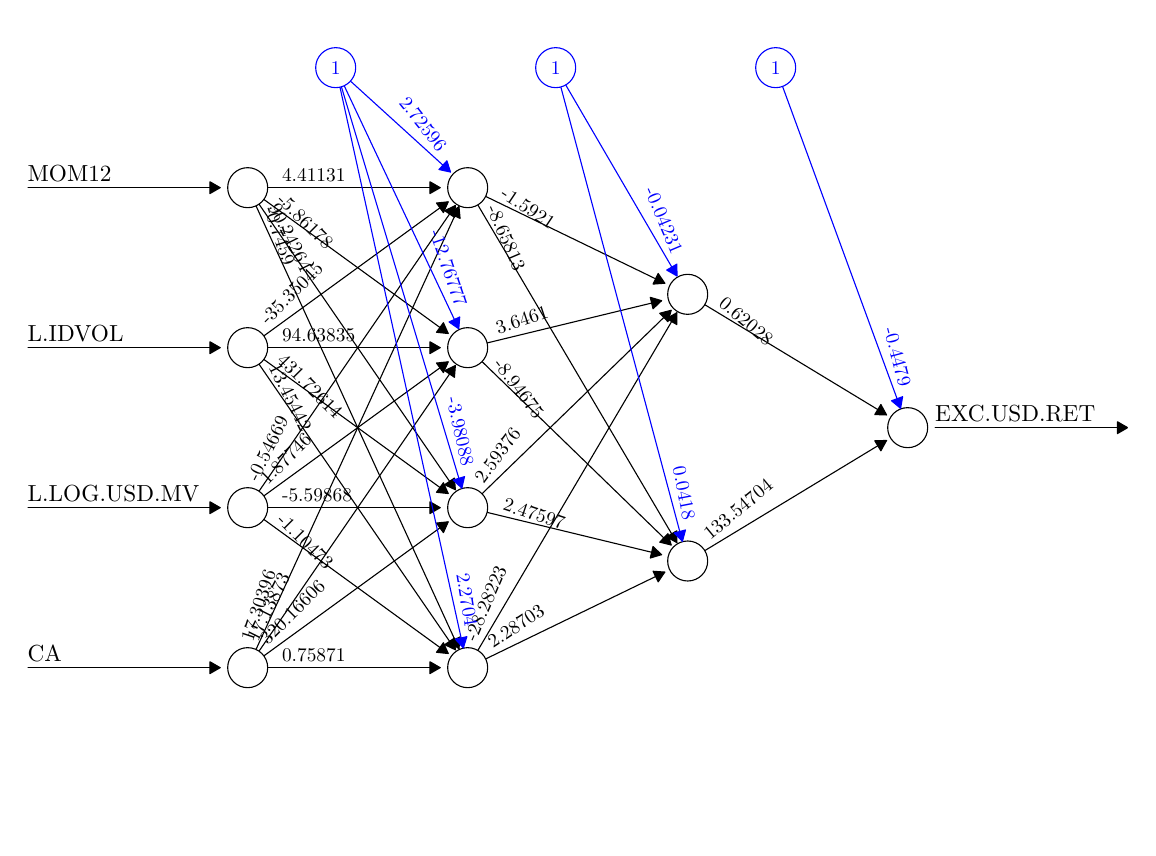
\begin{tikzpicture}[x=1pt,y=1pt]
\definecolor{fillColor}{RGB}{255,255,255}
\path[use as bounding box,fill=fillColor,fill opacity=0.00] (0,0) rectangle (397.48,289.08);
\begin{scope}
\path[clip] (  0.00,  0.00) rectangle (397.48,289.08);
\definecolor{drawColor}{RGB}{0,0,0}

\path[draw=drawColor,line width= 0.4pt,line join=round,line cap=round] ( 79.50, 57.82) --
	(149.06, 57.82);
\definecolor{fillColor}{RGB}{0,0,0}

\path[draw=drawColor,line width= 0.4pt,line join=round,line cap=round,fill=fillColor] (145.36, 55.68) --
	(149.06, 57.82) --
	(145.36, 59.95) --
	cycle;

\node[text=drawColor,anchor=base west,inner sep=0pt, outer sep=0pt, scale=  0.70] at ( 91.92, 59.95) {0.75871};
\end{scope}
\begin{scope}
\path[clip] (  0.00,  0.00) rectangle (397.48,289.08);
\definecolor{drawColor}{RGB}{0,0,0}

\path[draw=drawColor,line width= 0.4pt,line join=round,line cap=round] ( 79.50, 57.82) --
	(151.97,110.52);
\definecolor{fillColor}{RGB}{0,0,0}

\path[draw=drawColor,line width= 0.4pt,line join=round,line cap=round,fill=fillColor] (150.23,106.62) --
	(151.97,110.52) --
	(147.72,110.07) --
	cycle;

\node[text=drawColor,rotate= 45.00,anchor=base west,inner sep=0pt, outer sep=0pt, scale=  0.70] at ( 86.77, 65.71) {320.16606};
\end{scope}
\begin{scope}
\path[clip] (  0.00,  0.00) rectangle (397.48,289.08);
\definecolor{drawColor}{RGB}{0,0,0}

\path[draw=drawColor,line width= 0.4pt,line join=round,line cap=round] ( 79.50, 57.82) --
	(154.55,166.98);
\definecolor{fillColor}{RGB}{0,0,0}

\path[draw=drawColor,line width= 0.4pt,line join=round,line cap=round,fill=fillColor] (154.21,162.73) --
	(154.55,166.98) --
	(150.70,165.15) --
	cycle;

\node[text=drawColor,rotate= 63.43,anchor=base west,inner sep=0pt, outer sep=0pt, scale=  0.70] at ( 83.14, 66.85) {17.13873};
\end{scope}
\begin{scope}
\path[clip] (  0.00,  0.00) rectangle (397.48,289.08);
\definecolor{drawColor}{RGB}{0,0,0}

\path[draw=drawColor,line width= 0.4pt,line join=round,line cap=round] ( 79.50, 57.82) --
	(155.85,224.41);
\definecolor{fillColor}{RGB}{0,0,0}

\path[draw=drawColor,line width= 0.4pt,line join=round,line cap=round,fill=fillColor] (156.25,220.16) --
	(155.85,224.41) --
	(152.37,221.94) --
	cycle;

\node[text=drawColor,rotate= 71.57,anchor=base west,inner sep=0pt, outer sep=0pt, scale=  0.70] at ( 81.40, 67.06) {17.30396};
\end{scope}
\begin{scope}
\path[clip] (  0.00,  0.00) rectangle (397.48,289.08);
\definecolor{drawColor}{RGB}{0,0,0}

\path[draw=drawColor,line width= 0.4pt,line join=round,line cap=round] ( -0.00, 57.82) --
	( 69.56, 57.82);
\definecolor{fillColor}{RGB}{0,0,0}

\path[draw=drawColor,line width= 0.4pt,line join=round,line cap=round,fill=fillColor] ( 65.86, 55.68) --
	( 69.56, 57.82) --
	( 65.86, 59.95) --
	cycle;

\node[text=drawColor,anchor=base west,inner sep=0pt, outer sep=0pt, scale=  0.84] at ( -0.00, 59.95) {CA};
\end{scope}
\begin{scope}
\path[clip] (  0.00,  0.00) rectangle (397.48,289.08);
\definecolor{drawColor}{RGB}{0,0,0}
\definecolor{fillColor}{RGB}{255,255,255}

\path[draw=drawColor,line width= 0.4pt,line join=round,line cap=round,fill=fillColor] ( 79.50, 57.82) circle (  7.23);

\path[draw=drawColor,line width= 0.4pt,line join=round,line cap=round] ( 79.50,115.63) --
	(151.97, 62.93);
\definecolor{fillColor}{RGB}{0,0,0}

\path[draw=drawColor,line width= 0.4pt,line join=round,line cap=round,fill=fillColor] (147.72, 63.37) --
	(151.97, 62.93) --
	(150.23, 66.83) --
	cycle;

\node[text=drawColor,rotate=-45.00,anchor=base west,inner sep=0pt, outer sep=0pt, scale=  0.70] at ( 89.79,110.75) {-1.10473};
\end{scope}
\begin{scope}
\path[clip] (  0.00,  0.00) rectangle (397.48,289.08);
\definecolor{drawColor}{RGB}{0,0,0}

\path[draw=drawColor,line width= 0.4pt,line join=round,line cap=round] ( 79.50,115.63) --
	(149.06,115.63);
\definecolor{fillColor}{RGB}{0,0,0}

\path[draw=drawColor,line width= 0.4pt,line join=round,line cap=round,fill=fillColor] (145.36,113.50) --
	(149.06,115.63) --
	(145.36,117.77) --
	cycle;

\node[text=drawColor,anchor=base west,inner sep=0pt, outer sep=0pt, scale=  0.70] at ( 91.92,117.77) {-5.59868};
\end{scope}
\begin{scope}
\path[clip] (  0.00,  0.00) rectangle (397.48,289.08);
\definecolor{drawColor}{RGB}{0,0,0}

\path[draw=drawColor,line width= 0.4pt,line join=round,line cap=round] ( 79.50,115.63) --
	(151.97,168.34);
\definecolor{fillColor}{RGB}{0,0,0}

\path[draw=drawColor,line width= 0.4pt,line join=round,line cap=round,fill=fillColor] (150.23,164.44) --
	(151.97,168.34) --
	(147.72,167.89) --
	cycle;

\node[text=drawColor,rotate= 45.00,anchor=base west,inner sep=0pt, outer sep=0pt, scale=  0.70] at ( 86.77,123.53) {1.87746};
\end{scope}
\begin{scope}
\path[clip] (  0.00,  0.00) rectangle (397.48,289.08);
\definecolor{drawColor}{RGB}{0,0,0}

\path[draw=drawColor,line width= 0.4pt,line join=round,line cap=round] ( 79.50,115.63) --
	(154.55,224.80);
\definecolor{fillColor}{RGB}{0,0,0}

\path[draw=drawColor,line width= 0.4pt,line join=round,line cap=round,fill=fillColor] (154.21,220.55) --
	(154.55,224.80) --
	(150.70,222.96) --
	cycle;

\node[text=drawColor,rotate= 63.43,anchor=base west,inner sep=0pt, outer sep=0pt, scale=  0.70] at ( 83.14,124.67) {-0.54669};
\end{scope}
\begin{scope}
\path[clip] (  0.00,  0.00) rectangle (397.48,289.08);
\definecolor{drawColor}{RGB}{0,0,0}

\path[draw=drawColor,line width= 0.4pt,line join=round,line cap=round] ( -0.00,115.63) --
	( 69.56,115.63);
\definecolor{fillColor}{RGB}{0,0,0}

\path[draw=drawColor,line width= 0.4pt,line join=round,line cap=round,fill=fillColor] ( 65.86,113.50) --
	( 69.56,115.63) --
	( 65.86,117.77) --
	cycle;

\node[text=drawColor,anchor=base west,inner sep=0pt, outer sep=0pt, scale=  0.84] at ( -0.00,117.77) {L.LOG.USD.MV};
\end{scope}
\begin{scope}
\path[clip] (  0.00,  0.00) rectangle (397.48,289.08);
\definecolor{drawColor}{RGB}{0,0,0}
\definecolor{fillColor}{RGB}{255,255,255}

\path[draw=drawColor,line width= 0.4pt,line join=round,line cap=round,fill=fillColor] ( 79.50,115.63) circle (  7.23);

\path[draw=drawColor,line width= 0.4pt,line join=round,line cap=round] ( 79.50,173.45) --
	(154.55, 64.28);
\definecolor{fillColor}{RGB}{0,0,0}

\path[draw=drawColor,line width= 0.4pt,line join=round,line cap=round,fill=fillColor] (150.70, 66.12) --
	(154.55, 64.28) --
	(154.21, 68.53) --
	cycle;

\node[text=drawColor,rotate=-63.43,anchor=base west,inner sep=0pt, outer sep=0pt, scale=  0.70] at ( 86.96,166.32) {13.45442};
\end{scope}
\begin{scope}
\path[clip] (  0.00,  0.00) rectangle (397.48,289.08);
\definecolor{drawColor}{RGB}{0,0,0}

\path[draw=drawColor,line width= 0.4pt,line join=round,line cap=round] ( 79.50,173.45) --
	(151.97,120.74);
\definecolor{fillColor}{RGB}{0,0,0}

\path[draw=drawColor,line width= 0.4pt,line join=round,line cap=round,fill=fillColor] (147.72,121.19) --
	(151.97,120.74) --
	(150.23,124.64) --
	cycle;

\node[text=drawColor,rotate=-45.00,anchor=base west,inner sep=0pt, outer sep=0pt, scale=  0.70] at ( 89.79,168.57) {431.72614};
\end{scope}
\begin{scope}
\path[clip] (  0.00,  0.00) rectangle (397.48,289.08);
\definecolor{drawColor}{RGB}{0,0,0}

\path[draw=drawColor,line width= 0.4pt,line join=round,line cap=round] ( 79.50,173.45) --
	(149.06,173.45);
\definecolor{fillColor}{RGB}{0,0,0}

\path[draw=drawColor,line width= 0.4pt,line join=round,line cap=round,fill=fillColor] (145.36,171.31) --
	(149.06,173.45) --
	(145.36,175.58) --
	cycle;

\node[text=drawColor,anchor=base west,inner sep=0pt, outer sep=0pt, scale=  0.70] at ( 91.92,175.58) {94.63835};
\end{scope}
\begin{scope}
\path[clip] (  0.00,  0.00) rectangle (397.48,289.08);
\definecolor{drawColor}{RGB}{0,0,0}

\path[draw=drawColor,line width= 0.4pt,line join=round,line cap=round] ( 79.50,173.45) --
	(151.97,226.15);
\definecolor{fillColor}{RGB}{0,0,0}

\path[draw=drawColor,line width= 0.4pt,line join=round,line cap=round,fill=fillColor] (150.23,222.25) --
	(151.97,226.15) --
	(147.72,225.71) --
	cycle;

\node[text=drawColor,rotate= 45.00,anchor=base west,inner sep=0pt, outer sep=0pt, scale=  0.70] at ( 86.77,181.34) {-35.35045};
\end{scope}
\begin{scope}
\path[clip] (  0.00,  0.00) rectangle (397.48,289.08);
\definecolor{drawColor}{RGB}{0,0,0}

\path[draw=drawColor,line width= 0.4pt,line join=round,line cap=round] ( -0.00,173.45) --
	( 69.56,173.45);
\definecolor{fillColor}{RGB}{0,0,0}

\path[draw=drawColor,line width= 0.4pt,line join=round,line cap=round,fill=fillColor] ( 65.86,171.31) --
	( 69.56,173.45) --
	( 65.86,175.58) --
	cycle;

\node[text=drawColor,anchor=base west,inner sep=0pt, outer sep=0pt, scale=  0.84] at ( -0.00,175.58) {L.IDVOL};
\end{scope}
\begin{scope}
\path[clip] (  0.00,  0.00) rectangle (397.48,289.08);
\definecolor{drawColor}{RGB}{0,0,0}
\definecolor{fillColor}{RGB}{255,255,255}

\path[draw=drawColor,line width= 0.4pt,line join=round,line cap=round,fill=fillColor] ( 79.50,173.45) circle (  7.23);

\path[draw=drawColor,line width= 0.4pt,line join=round,line cap=round] ( 79.50,231.26) --
	(155.85, 64.67);
\definecolor{fillColor}{RGB}{0,0,0}

\path[draw=drawColor,line width= 0.4pt,line join=round,line cap=round,fill=fillColor] (152.37, 67.14) --
	(155.85, 64.67) --
	(156.25, 68.92) --
	cycle;

\node[text=drawColor,rotate=-71.57,anchor=base west,inner sep=0pt, outer sep=0pt, scale=  0.70] at ( 85.45,223.37) {-0.7459};
\end{scope}
\begin{scope}
\path[clip] (  0.00,  0.00) rectangle (397.48,289.08);
\definecolor{drawColor}{RGB}{0,0,0}

\path[draw=drawColor,line width= 0.4pt,line join=round,line cap=round] ( 79.50,231.26) --
	(154.55,122.10);
\definecolor{fillColor}{RGB}{0,0,0}

\path[draw=drawColor,line width= 0.4pt,line join=round,line cap=round,fill=fillColor] (150.70,123.93) --
	(154.55,122.10) --
	(154.21,126.35) --
	cycle;

\node[text=drawColor,rotate=-63.43,anchor=base west,inner sep=0pt, outer sep=0pt, scale=  0.70] at ( 86.96,224.14) {90.24264};
\end{scope}
\begin{scope}
\path[clip] (  0.00,  0.00) rectangle (397.48,289.08);
\definecolor{drawColor}{RGB}{0,0,0}

\path[draw=drawColor,line width= 0.4pt,line join=round,line cap=round] ( 79.50,231.26) --
	(151.97,178.56);
\definecolor{fillColor}{RGB}{0,0,0}

\path[draw=drawColor,line width= 0.4pt,line join=round,line cap=round,fill=fillColor] (147.72,179.01) --
	(151.97,178.56) --
	(150.23,182.46) --
	cycle;

\node[text=drawColor,rotate=-45.00,anchor=base west,inner sep=0pt, outer sep=0pt, scale=  0.70] at ( 89.79,226.39) {-5.86178};
\end{scope}
\begin{scope}
\path[clip] (  0.00,  0.00) rectangle (397.48,289.08);
\definecolor{drawColor}{RGB}{0,0,0}

\path[draw=drawColor,line width= 0.4pt,line join=round,line cap=round] ( 79.50,231.26) --
	(149.06,231.26);
\definecolor{fillColor}{RGB}{0,0,0}

\path[draw=drawColor,line width= 0.4pt,line join=round,line cap=round,fill=fillColor] (145.36,229.13) --
	(149.06,231.26) --
	(145.36,233.40) --
	cycle;

\node[text=drawColor,anchor=base west,inner sep=0pt, outer sep=0pt, scale=  0.70] at ( 91.92,233.40) {4.41131};
\end{scope}
\begin{scope}
\path[clip] (  0.00,  0.00) rectangle (397.48,289.08);
\definecolor{drawColor}{RGB}{0,0,0}

\path[draw=drawColor,line width= 0.4pt,line join=round,line cap=round] ( -0.00,231.26) --
	( 69.56,231.26);
\definecolor{fillColor}{RGB}{0,0,0}

\path[draw=drawColor,line width= 0.4pt,line join=round,line cap=round,fill=fillColor] ( 65.86,229.13) --
	( 69.56,231.26) --
	( 65.86,233.40) --
	cycle;

\node[text=drawColor,anchor=base west,inner sep=0pt, outer sep=0pt, scale=  0.84] at ( -0.00,233.40) {MOM12};
\end{scope}
\begin{scope}
\path[clip] (  0.00,  0.00) rectangle (397.48,289.08);
\definecolor{drawColor}{RGB}{0,0,0}
\definecolor{fillColor}{RGB}{255,255,255}

\path[draw=drawColor,line width= 0.4pt,line join=round,line cap=round,fill=fillColor] ( 79.50,231.26) circle (  7.23);

\path[draw=drawColor,line width= 0.4pt,line join=round,line cap=round] (158.99, 57.82) --
	(230.22, 92.35);
\definecolor{fillColor}{RGB}{0,0,0}

\path[draw=drawColor,line width= 0.4pt,line join=round,line cap=round,fill=fillColor] (227.83, 88.82) --
	(230.22, 92.35) --
	(225.97, 92.66) --
	cycle;

\node[text=drawColor,rotate= 33.69,anchor=base west,inner sep=0pt, outer sep=0pt, scale=  0.70] at (168.15, 64.60) {2.28703};
\end{scope}
\begin{scope}
\path[clip] (  0.00,  0.00) rectangle (397.48,289.08);
\definecolor{drawColor}{RGB}{0,0,0}

\path[draw=drawColor,line width= 0.4pt,line join=round,line cap=round] (158.99, 57.82) --
	(234.58,186.08);
\definecolor{fillColor}{RGB}{0,0,0}

\path[draw=drawColor,line width= 0.4pt,line join=round,line cap=round,fill=fillColor] (234.54,181.81) --
	(234.58,186.08) --
	(230.86,183.98) --
	cycle;

\node[text=drawColor,rotate= 66.80,anchor=base west,inner sep=0pt, outer sep=0pt, scale=  0.70] at (161.93, 66.96) {-28.28223};
\end{scope}
\begin{scope}
\path[clip] (  0.00,  0.00) rectangle (397.48,289.08);
\definecolor{drawColor}{RGB}{0,0,0}
\definecolor{fillColor}{RGB}{255,255,255}

\path[draw=drawColor,line width= 0.4pt,line join=round,line cap=round,fill=fillColor] (158.99, 57.82) circle (  7.23);

\path[draw=drawColor,line width= 0.4pt,line join=round,line cap=round] (158.99,115.63) --
	(229.06, 98.65);
\definecolor{fillColor}{RGB}{0,0,0}

\path[draw=drawColor,line width= 0.4pt,line join=round,line cap=round,fill=fillColor] (224.97, 97.44) --
	(229.06, 98.65) --
	(225.97,101.59) --
	cycle;

\node[text=drawColor,rotate=-18.43,anchor=base west,inner sep=0pt, outer sep=0pt, scale=  0.70] at (171.45,114.80) {2.47597};
\end{scope}
\begin{scope}
\path[clip] (  0.00,  0.00) rectangle (397.48,289.08);
\definecolor{drawColor}{RGB}{0,0,0}

\path[draw=drawColor,line width= 0.4pt,line join=round,line cap=round] (158.99,115.63) --
	(232.53,186.94);
\definecolor{fillColor}{RGB}{0,0,0}

\path[draw=drawColor,line width= 0.4pt,line join=round,line cap=round,fill=fillColor] (231.36,182.83) --
	(232.53,186.94) --
	(228.39,185.90) --
	cycle;

\node[text=drawColor,rotate= 53.13,anchor=base west,inner sep=0pt, outer sep=0pt, scale=  0.70] at (164.74,124.14) {2.59376};
\end{scope}
\begin{scope}
\path[clip] (  0.00,  0.00) rectangle (397.48,289.08);
\definecolor{drawColor}{RGB}{0,0,0}
\definecolor{fillColor}{RGB}{255,255,255}

\path[draw=drawColor,line width= 0.4pt,line join=round,line cap=round,fill=fillColor] (158.99,115.63) circle (  7.23);

\path[draw=drawColor,line width= 0.4pt,line join=round,line cap=round] (158.99,173.45) --
	(232.53,102.14);
\definecolor{fillColor}{RGB}{0,0,0}

\path[draw=drawColor,line width= 0.4pt,line join=round,line cap=round,fill=fillColor] (228.39,103.18) --
	(232.53,102.14) --
	(231.36,106.25) --
	cycle;

\node[text=drawColor,rotate=-53.13,anchor=base west,inner sep=0pt, outer sep=0pt, scale=  0.70] at (168.15,167.50) {-8.94675};
\end{scope}
\begin{scope}
\path[clip] (  0.00,  0.00) rectangle (397.48,289.08);
\definecolor{drawColor}{RGB}{0,0,0}

\path[draw=drawColor,line width= 0.4pt,line join=round,line cap=round] (158.99,173.45) --
	(229.06,190.43);
\definecolor{fillColor}{RGB}{0,0,0}

\path[draw=drawColor,line width= 0.4pt,line join=round,line cap=round,fill=fillColor] (225.97,187.49) --
	(229.06,190.43) --
	(224.97,191.64) --
	cycle;

\node[text=drawColor,rotate= 18.43,anchor=base west,inner sep=0pt, outer sep=0pt, scale=  0.70] at (170.10,178.33) {3.6461};
\end{scope}
\begin{scope}
\path[clip] (  0.00,  0.00) rectangle (397.48,289.08);
\definecolor{drawColor}{RGB}{0,0,0}
\definecolor{fillColor}{RGB}{255,255,255}

\path[draw=drawColor,line width= 0.4pt,line join=round,line cap=round,fill=fillColor] (158.99,173.45) circle (  7.23);

\path[draw=drawColor,line width= 0.4pt,line join=round,line cap=round] (158.99,231.26) --
	(234.58,103.00);
\definecolor{fillColor}{RGB}{0,0,0}

\path[draw=drawColor,line width= 0.4pt,line join=round,line cap=round,fill=fillColor] (230.86,105.10) --
	(234.58,103.00) --
	(234.54,107.27) --
	cycle;

\node[text=drawColor,rotate=-66.80,anchor=base west,inner sep=0pt, outer sep=0pt, scale=  0.70] at (165.85,223.80) {-8.65813};
\end{scope}
\begin{scope}
\path[clip] (  0.00,  0.00) rectangle (397.48,289.08);
\definecolor{drawColor}{RGB}{0,0,0}

\path[draw=drawColor,line width= 0.4pt,line join=round,line cap=round] (158.99,231.26) --
	(230.22,196.73);
\definecolor{fillColor}{RGB}{0,0,0}

\path[draw=drawColor,line width= 0.4pt,line join=round,line cap=round,fill=fillColor] (225.97,196.42) --
	(230.22,196.73) --
	(227.83,200.26) --
	cycle;

\node[text=drawColor,rotate=-33.69,anchor=base west,inner sep=0pt, outer sep=0pt, scale=  0.70] at (170.51,228.03) {-1.5921};
\end{scope}
\begin{scope}
\path[clip] (  0.00,  0.00) rectangle (397.48,289.08);
\definecolor{drawColor}{RGB}{0,0,0}
\definecolor{fillColor}{RGB}{255,255,255}

\path[draw=drawColor,line width= 0.4pt,line join=round,line cap=round,fill=fillColor] (158.99,231.26) circle (  7.23);

\path[draw=drawColor,line width= 0.4pt,line join=round,line cap=round] (238.49, 96.36) --
	(310.35,139.91);
\definecolor{fillColor}{RGB}{0,0,0}

\path[draw=drawColor,line width= 0.4pt,line join=round,line cap=round,fill=fillColor] (308.30,136.17) --
	(310.35,139.91) --
	(306.09,139.82) --
	cycle;

\node[text=drawColor,rotate= 39.81,anchor=base west,inner sep=0pt, outer sep=0pt, scale=  0.70] at (246.67,103.78) {133.54704};
\end{scope}
\begin{scope}
\path[clip] (  0.00,  0.00) rectangle (397.48,289.08);
\definecolor{drawColor}{RGB}{0,0,0}
\definecolor{fillColor}{RGB}{255,255,255}

\path[draw=drawColor,line width= 0.4pt,line join=round,line cap=round,fill=fillColor] (238.49, 96.36) circle (  7.23);

\path[draw=drawColor,line width= 0.4pt,line join=round,line cap=round] (238.49,192.72) --
	(310.35,149.17);
\definecolor{fillColor}{RGB}{0,0,0}

\path[draw=drawColor,line width= 0.4pt,line join=round,line cap=round,fill=fillColor] (306.09,149.26) --
	(310.35,149.17) --
	(308.30,152.91) --
	cycle;

\node[text=drawColor,rotate=-39.81,anchor=base west,inner sep=0pt, outer sep=0pt, scale=  0.70] at (249.40,188.58) {0.62028};
\end{scope}
\begin{scope}
\path[clip] (  0.00,  0.00) rectangle (397.48,289.08);
\definecolor{drawColor}{RGB}{0,0,0}
\definecolor{fillColor}{RGB}{255,255,255}

\path[draw=drawColor,line width= 0.4pt,line join=round,line cap=round,fill=fillColor] (238.49,192.72) circle (  7.23);

\path[draw=drawColor,line width= 0.4pt,line join=round,line cap=round] (327.93,144.54) --
	(397.48,144.54);
\definecolor{fillColor}{RGB}{0,0,0}

\path[draw=drawColor,line width= 0.4pt,line join=round,line cap=round,fill=fillColor] (393.79,142.41) --
	(397.48,144.54) --
	(393.79,146.67) --
	cycle;

\node[text=drawColor,anchor=base west,inner sep=0pt, outer sep=0pt, scale=  0.84] at (327.93,146.67) {EXC.USD.RET};
\end{scope}
\begin{scope}
\path[clip] (  0.00,  0.00) rectangle (397.48,289.08);
\definecolor{drawColor}{RGB}{0,0,0}
\definecolor{fillColor}{RGB}{255,255,255}

\path[draw=drawColor,line width= 0.4pt,line join=round,line cap=round,fill=fillColor] (317.99,144.54) circle (  7.23);
\definecolor{drawColor}{RGB}{0,0,255}

\path[draw=drawColor,line width= 0.4pt,line join=round,line cap=round] (111.30,274.63) --
	(157.42, 64.95);
\definecolor{fillColor}{RGB}{0,0,255}

\path[draw=drawColor,line width= 0.4pt,line join=round,line cap=round,fill=fillColor] (154.55, 68.10) --
	(157.42, 64.95) --
	(158.71, 69.02) --
	cycle;

\node[text=drawColor,rotate=-80.91,anchor=base east,inner sep=0pt, outer sep=0pt, scale=  0.70] at (157.96, 72.43) {2.2704};
\end{scope}
\begin{scope}
\path[clip] (  0.00,  0.00) rectangle (397.48,289.08);
\definecolor{drawColor}{RGB}{0,0,255}

\path[draw=drawColor,line width= 0.4pt,line join=round,line cap=round] (111.30,274.63) --
	(156.88,122.69);
\definecolor{fillColor}{RGB}{0,0,255}

\path[draw=drawColor,line width= 0.4pt,line join=round,line cap=round,fill=fillColor] (153.77,125.62) --
	(156.88,122.69) --
	(157.86,126.85) --
	cycle;

\node[text=drawColor,rotate=-77.69,anchor=base east,inner sep=0pt, outer sep=0pt, scale=  0.70] at (156.84,130.21) {-3.98088};
\end{scope}
\begin{scope}
\path[clip] (  0.00,  0.00) rectangle (397.48,289.08);
\definecolor{drawColor}{RGB}{0,0,255}

\path[draw=drawColor,line width= 0.4pt,line join=round,line cap=round] (111.30,274.63) --
	(155.77,180.28);
\definecolor{fillColor}{RGB}{0,0,255}

\path[draw=drawColor,line width= 0.4pt,line join=round,line cap=round,fill=fillColor] (152.26,182.72) --
	(155.77,180.28) --
	(156.13,184.54) --
	cycle;

\node[text=drawColor,rotate=-71.08,anchor=base east,inner sep=0pt, outer sep=0pt, scale=  0.70] at (154.57,187.81) {-12.76777};
\end{scope}
\begin{scope}
\path[clip] (  0.00,  0.00) rectangle (397.48,289.08);
\definecolor{drawColor}{RGB}{0,0,255}

\path[draw=drawColor,line width= 0.4pt,line join=round,line cap=round] (111.30,274.63) --
	(152.79,236.91);
\definecolor{fillColor}{RGB}{0,0,255}

\path[draw=drawColor,line width= 0.4pt,line join=round,line cap=round,fill=fillColor] (148.62,237.81) --
	(152.79,236.91) --
	(151.49,240.97) --
	cycle;

\node[text=drawColor,rotate=-51.34,anchor=base east,inner sep=0pt, outer sep=0pt, scale=  0.70] at (148.24,243.88) {2.72596};
\end{scope}
\begin{scope}
\path[clip] (  0.00,  0.00) rectangle (397.48,289.08);
\definecolor{drawColor}{RGB}{0,0,255}
\definecolor{fillColor}{RGB}{255,255,255}

\path[draw=drawColor,line width= 0.4pt,line join=round,line cap=round,fill=fillColor] (111.30,274.63) circle (  7.23);

\node[text=drawColor,anchor=base,inner sep=0pt, outer sep=0pt, scale=  0.70] at (111.30,272.22) {1};

\path[draw=drawColor,line width= 0.4pt,line join=round,line cap=round] (190.79,274.63) --
	(236.59,103.45);
\definecolor{fillColor}{RGB}{0,0,255}

\path[draw=drawColor,line width= 0.4pt,line join=round,line cap=round,fill=fillColor] (233.58,106.47) --
	(236.59,103.45) --
	(237.70,107.58) --
	cycle;

\node[text=drawColor,rotate=-78.99,anchor=base east,inner sep=0pt, outer sep=0pt, scale=  0.70] at (236.79,110.96) {0.0418};
\end{scope}
\begin{scope}
\path[clip] (  0.00,  0.00) rectangle (397.48,289.08);
\definecolor{drawColor}{RGB}{0,0,255}

\path[draw=drawColor,line width= 0.4pt,line join=round,line cap=round] (190.79,274.63) --
	(234.62,199.37);
\definecolor{fillColor}{RGB}{0,0,255}

\path[draw=drawColor,line width= 0.4pt,line join=round,line cap=round,fill=fillColor] (230.91,201.49) --
	(234.62,199.37) --
	(234.60,203.64) --
	cycle;

\node[text=drawColor,rotate=-67.05,anchor=base east,inner sep=0pt, outer sep=0pt, scale=  0.70] at (232.71,206.86) {-0.04231};
\end{scope}
\begin{scope}
\path[clip] (  0.00,  0.00) rectangle (397.48,289.08);
\definecolor{drawColor}{RGB}{0,0,255}
\definecolor{fillColor}{RGB}{255,255,255}

\path[draw=drawColor,line width= 0.4pt,line join=round,line cap=round,fill=fillColor] (190.79,274.63) circle (  7.23);

\node[text=drawColor,anchor=base,inner sep=0pt, outer sep=0pt, scale=  0.70] at (190.79,272.22) {1};

\path[draw=drawColor,line width= 0.4pt,line join=round,line cap=round] (270.29,274.63) --
	(315.43,151.52);
\definecolor{fillColor}{RGB}{0,0,255}

\path[draw=drawColor,line width= 0.4pt,line join=round,line cap=round,fill=fillColor] (312.15,154.26) --
	(315.43,151.52) --
	(316.16,155.73) --
	cycle;

\node[text=drawColor,rotate=-75.07,anchor=base east,inner sep=0pt, outer sep=0pt, scale=  0.70] at (314.93,159.06) {-0.4479};
\end{scope}
\begin{scope}
\path[clip] (  0.00,  0.00) rectangle (397.48,289.08);
\definecolor{drawColor}{RGB}{0,0,255}
\definecolor{fillColor}{RGB}{255,255,255}

\path[draw=drawColor,line width= 0.4pt,line join=round,line cap=round,fill=fillColor] (270.29,274.63) circle (  7.23);

\node[text=drawColor,anchor=base,inner sep=0pt, outer sep=0pt, scale=  0.70] at (270.29,272.22) {1};
\end{scope}
\end{tikzpicture}

\label{plot:NN}
\end{figure}

\section{Empirical results on Nordic equitites}

Performance of the machine learning models will be evaluated from two aspects. First profitability of the models will be evaluated by investigating performance of univariate expected return sort portfolios. Construction of these portfolios is explained in more detail in section \ref{Methodology}. Second aspect that is examined is the prediction accuracy of the machine learning models. Prediction accuracy is evaluated by out-out sample $R^2$. Additionally, in the spirit of Lewellen \citeyear{lewellen2015} relationship between expected and realized excess returns are examined by regressing the realized excess returns with the individual stock level predicted returns. Finally, the variable importance for different methods are calculated to see effect of each explanatory variable to the prediction accuracy of the model. Process to define variable importance is described in section \ref{VariableImportance}.

\subsection{Portfolio performance}

\subsection{Predictive performance}

\subsection{Variable importance}

Table \ref{table:PortfolioPerformance}

\begin{table}[h]
\small
\caption[Machine learning portfolio performance]{\textbf{Machine learning portfolio performance} \\ Table reports performance metrics for portfolios formed based on univariate expected return sort. Each month all stocks are allocated to ten portfolios based on their expected returns. Breakpoints for the allocation are calculated only from big stocks, which are the biggest stocks that in current month account for 90 percent of cumulative market value of all stocks in the dataset. H-L is zero investment portfolio which consist of short position in portfolio formed from stocks with lowest expected return and long position in portfolio formed from stocks with highest expected return. Time series average of predicted return and realized return of each portfolio is reported for each portfolio together with standard error of realized return. Additionally, Sharpe ratios are reported. Panel A reports result for equally weighted portfolios and panel B reports results for portfolios where each stock in portfolio is weighted by its lagged market value.}
\label{table:PortfolioPerformance}
\centering
\newcolumntype{Y}{>{\centering\arraybackslash}X}
\begin{tabularx}{\textwidth}{@{\extracolsep{1pt}} l Y Y Y Y Y Y Y Y Y Y Y Y} 
\toprule
\multicolumn{13}{l}{\textit{Panel A: Equal weighted}}\\
\midrule
& \multicolumn{4}{c}{FM} & \multicolumn{4}{c}{RF} & \multicolumn{4}{c}{NN} \\
\cline{2-5}\cline{6-9}\cline{10-13}
			& Pred 	& Avg 	& SE 	& SR 	& Pred 	& Avg 	& SE 	& SR  	& Pred 	& Avg 	& SE 	& SR  \\
\midrule
Low			& -0.0042 	& 0.0037 	& 0.004	& 0.05 	& -0.0067 	& -0.0016	& 0.004 	& -0.02 	& -0.0148	& 0.0004 	& 0.004	& 0.01\\
2			& 0.0025	& 0.0045 	& 0.004	& 0.07 	& 0.0006 	& 0.0053	& 0.004 	& 0.08 	& -0.0029	& 0.0065 	& 0.004 	& 0.10\\
3		 	& 0.0050 	& 0.0055 	& 0.004	& 0.09 	& 0.0033 	& 0.0060	& 0.004 	& 0.10 	& 0.0010	& 0.0056 	& 0.003	& 0.09\\
4 			& 0.0068 	& 0.0069 	& 0.003	& 0.11 	& 0.0056 	& 0.0107	& 0.003 	& 0.17 	& 0.0040	& 0.0084 	& 0.003 	& 0.14\\
5 			& 0.0083	& 0.0090 	& 0.003	& 0.15 	& 0.0077	& 0.0095	& 0.003 	& 0.16 	& 0.0066	& 0.0085	& 0.003	& 0.14\\
6			& 0.0099	& 0.0082 	& 0.003	& 0.14 	& 0.0098 	& 0.0081	& 0.003 	& 0.13 	& 0.0090	& 0.0094 	& 0.003	& 0.15\\
7			& 0.0116 	& 0.0100 	& 0.003	& 0.16 	& 0.0117	& 0.0098	& 0.003	& 0.16 	& 0.0114	& 0.0103 	& 0.003	& 0.17\\
8			& 0.0138	& 0.0115 	& 0.004	& 0.18 	& 0.0136	& 0.0121	& 0.003 	& 0.19 	& 0.0142	& 0.0108 	& 0.003 	& 0.17\\
9			& 0.0171 	& 0.0118 	& 0.004	& 0.19 	& 0.0159	& 0.0142	& 0.003 	& 0.23 	& 0.0179	& 0.0129 	& 0.003 	& 0.20\\
High			& 0.0300	& 0.0180 	& 0.004	& 0.26	& 0.0235	& 0.0178	& 0.004 	& 0.25 	& 0.0282	& 0.0142 	& 0.004 	& 0.21\\
H-L			& 0.0342	& 0.0143 	& 0.003	& 0.27	& 0.0303	& 0.0194	& 0.002	& 0.48 	& 0.0430	& 0.0138 	& 0.002 	& 0.330\\
\toprule
\multicolumn{13}{l}{\textit{Panel B: Value weighted}}\\
\midrule
& \multicolumn{4}{c}{FM} & \multicolumn{4}{c}{RF} & \multicolumn{4}{c}{NN} \\
\cline{2-5}\cline{6-9}\cline{10-13}
			& Pred 	& Avg 	& SE 	& SR 	& Pred 	& Avg 	& SE 	& SR  	& Pred 	& Avg 	& SE		& SR  \\
\midrule
Low			& -0.0033	& 0.0075 	& 0.004	& 0.10 	& -0.0056 	& 0.0017	& 0.004	& 0.02 	& -0.0126	& 0.0062 	& 0.004 	& 0.08\\
2			& 0.0025	& 0.0054 	& 0.004	& 0.08 	& 0.0006 	& 0.0058	& 0.004	& 0.09 	& -0.0029	& 0.0058 	& 0.004 	& 0.08\\
3		 	& 0.0050	& 0.0073 	& 0.004	& 0.11 	& 0.0033	& 0.0072	& 0.004	& 0.11 	& 0.0010	& 0.0063	& 0.004 	& 0.10\\
4 			& 0.0068	& 0.0083 	& 0.004	& 0.13 	& 0.0056	& 0.0093	& 0.004	& 0.15 	& 0.0040	& 0.0096 	& 0.004 	& 0.15\\
5 			& 0.0083	& 0.0085 	& 0.003	& 0.13 	& 0.0078 	& 0.0106	& 0.004	& 0.17 	& 0.0066	& 0.0080	& 0.003 	& 0.13\\
6			& 0.0099	& 0.0080 	& 0.003	& 0.13 	& 0.0098 	& 0.0054	& 0.004	& 0.08 	& 0.0090	& 0.0092 	& 0.003 	& 0.15\\
7			& 0.0116	& 0.0065 	& 0.003	& 0.11 	& 0.0117 	& 0.0070	& 0.004	& 0.11 	& 0.0114	& 0.0088	& 0.003 	& 0.14\\
8			& 0.0138	& 0.0084 	& 0.004	& 0.13 	& 0.0136 	& 0.0097	& 0.004	& 0.15 	& 0.0142	& 0.0094 	& 0.004 	& 0.14\\
9			& 0.0171	& 0.0089 	& 0.004	& 0.14 	& 0.0159 	& 0.0125	& 0.004	& 0.19 	& 0.0179	& 0.0108 	& 0.004 	& 0.17\\
High			& 0.0313	& 0.0142 	& 0.004	& 0.21 	& 0.0219 	& 0.0140	& 0.004	& 0.18 	& 0.0283	& 0.0138 	& 0.004 	& 0.19\\
H-L			& 0.0347	& 0.0067 	& 0.003	& 0.11 	& 0.0275 	& 0.0123	& 0.003	& 0.24 	& 0.0409	& 0.0076 	& 0.003 	& 0.14\\
\bottomrule
\end{tabularx}
\end{table}

\begin{table}[h]
\small
\caption[Zero investment portfolio performance metrics]{\textbf{Zero investment portfolio performance metrics} \\ ...}
\label{table:PortfolioPerformanceMetrics}
\centering
\newcolumntype{Y}{>{\centering\arraybackslash}X}
\begin{tabularx}{\textwidth}{@{\extracolsep{4pt}} l Y Y Y Y Y Y} 
\toprule
& \multicolumn{3}{c}{Equal weighted} & \multicolumn{3}{c}{Value weighted} \\
\cline{2-4}\cline{5-7}\cline{6-7}
					& FM 	& RF 	& NN 	& FM 	& RF 	& NN \\
\midrule
Max DD(\%) 			& -0.4504573	& -0.1888231 	& -0.3822367	& -0.5707584 	& -0.2706739 	& -0.4916363\\
Max 1month Loss(\%) 	& -0.1988272 	& -0.1151289	&  -0.2061243	& -0.3200514 	& -0.1893646 & -0.3592626\\
FF Alpha 				& 0.0048553 & 0.0148573	 & 0.0092023 & -0.0039026 & 0.0075169 & 0.0006789\\
t-stats 				& 2.4673874 & 6.9306208 & 4.5004057 & -1.6110870  & 2.6993460 & 0.2422617\\
$R^2$ 				& 0.5928532 & 0.1609467	& 0.2930559 & 0.5230763 & 0.1342177 & 0.2623851\\
Sharpe ratio			& 0.2690346 & 0.4808831	& 0.3303232 & 0.1104301 & 0.2377289 & 0.1352148\\
Turnover (\%)		 	& 0.10756625 & 0.11414496 & 0.12479359 & 0.09903494 & 0.14775978 	& 0.13905048\\
\bottomrule
\end{tabularx}
\end{table}

\begin{figure}[h]
\centering
\caption[Cumulative return of machine learning portfolios]{\textbf{..}\\ ...}
% Created by tikzDevice version 0.12.6 on 2024-03-28 21:54:17
% !TEX encoding = UTF-8 Unicode
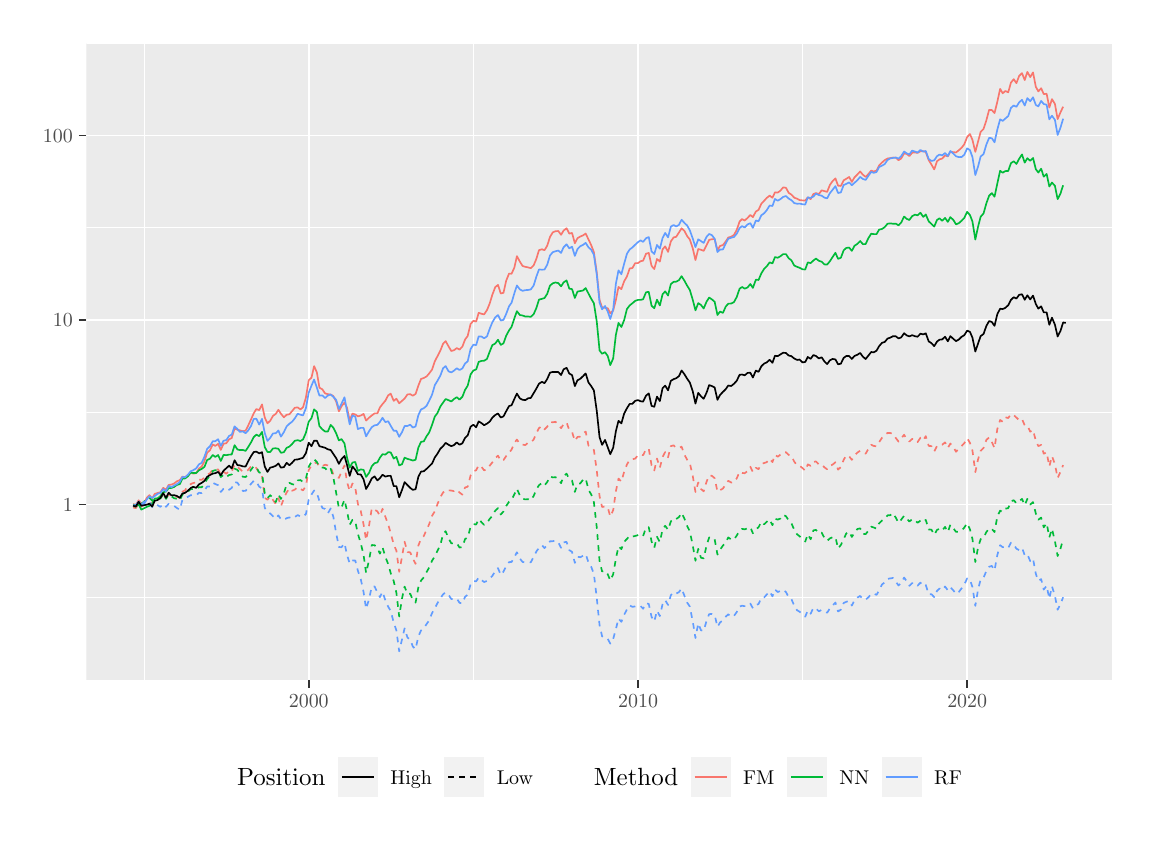
\begin{tikzpicture}[x=1pt,y=1pt]
\definecolor{fillColor}{RGB}{255,255,255}
\path[use as bounding box,fill=fillColor,fill opacity=0.00] (0,0) rectangle (397.48,289.08);
\begin{scope}
\path[clip] (  0.00,  0.00) rectangle (397.48,289.08);
\definecolor{drawColor}{RGB}{255,255,255}
\definecolor{fillColor}{RGB}{255,255,255}

\path[draw=drawColor,line width= 0.6pt,line join=round,line cap=round,fill=fillColor] (  0.00,  0.00) rectangle (397.48,289.08);
\end{scope}
\begin{scope}
\path[clip] ( 21.25, 53.26) rectangle (391.98,283.58);
\definecolor{fillColor}{gray}{0.92}

\path[fill=fillColor] ( 21.25, 53.26) rectangle (391.98,283.58);
\definecolor{drawColor}{RGB}{255,255,255}

\path[draw=drawColor,line width= 0.3pt,line join=round] ( 21.25, 83.37) --
	(391.98, 83.37);

\path[draw=drawColor,line width= 0.3pt,line join=round] ( 21.25,150.09) --
	(391.98,150.09);

\path[draw=drawColor,line width= 0.3pt,line join=round] ( 21.25,216.81) --
	(391.98,216.81);

\path[draw=drawColor,line width= 0.3pt,line join=round] ( 21.25,283.53) --
	(391.98,283.53);

\path[draw=drawColor,line width= 0.3pt,line join=round] ( 42.09, 53.26) --
	( 42.09,283.58);

\path[draw=drawColor,line width= 0.3pt,line join=round] (161.07, 53.26) --
	(161.07,283.58);

\path[draw=drawColor,line width= 0.3pt,line join=round] (280.03, 53.26) --
	(280.03,283.58);

\path[draw=drawColor,line width= 0.6pt,line join=round] ( 21.25,116.73) --
	(391.98,116.73);

\path[draw=drawColor,line width= 0.6pt,line join=round] ( 21.25,183.45) --
	(391.98,183.45);

\path[draw=drawColor,line width= 0.6pt,line join=round] ( 21.25,250.17) --
	(391.98,250.17);

\path[draw=drawColor,line width= 0.6pt,line join=round] (101.58, 53.26) --
	(101.58,283.58);

\path[draw=drawColor,line width= 0.6pt,line join=round] (220.56, 53.26) --
	(220.56,283.58);

\path[draw=drawColor,line width= 0.6pt,line join=round] (339.50, 53.26) --
	(339.50,283.58);
\definecolor{drawColor}{RGB}{248,118,109}

\path[draw=drawColor,line width= 0.6pt,line join=round] ( 38.10,116.96) --
	( 39.08,116.60) --
	( 40.09,118.30) --
	( 41.06,117.16) --
	( 42.04,117.41) --
	( 43.08,119.22) --
	( 43.99,120.15) --
	( 45.00,119.00) --
	( 45.92,120.62) --
	( 46.99,120.96) --
	( 47.97,121.21) --
	( 48.98,122.79) --
	( 49.99,122.10) --
	( 50.93,123.85) --
	( 51.97,123.98) --
	( 52.95,124.38) --
	( 53.90,125.16) --
	( 54.97,125.57) --
	( 55.91,126.84) --
	( 56.86,126.68) --
	( 57.90,127.37) --
	( 58.91,128.33) --
	( 59.82,127.92) --
	( 60.90,128.10) --
	( 61.88,129.76) --
	( 62.88,130.48) --
	( 63.89,132.43) --
	( 64.84,135.43) --
	( 65.88,136.41) --
	( 66.89,138.45) --
	( 67.80,137.96) --
	( 68.81,138.68) --
	( 69.79,136.49) --
	( 70.77,138.71) --
	( 71.78,138.93) --
	( 72.79,140.32) --
	( 73.73,140.79) --
	( 74.77,144.25) --
	( 75.78,143.79) --
	( 76.69,143.56) --
	( 77.77,143.27) --
	( 78.75,143.46) --
	( 79.66,145.26) --
	( 80.70,147.50) --
	( 81.68,149.72) --
	( 82.62,151.27) --
	( 83.66,150.88) --
	( 84.67,152.95) --
	( 85.68,148.16) --
	( 86.66,146.12) --
	( 87.64,147.04) --
	( 88.65,148.81) --
	( 89.66,149.53) --
	( 90.60,151.00) --
	( 91.51,149.57) --
	( 92.59,148.28) --
	( 93.57,149.19) --
	( 94.58,149.39) --
	( 95.55,150.53) --
	( 96.53,151.74) --
	( 97.57,151.86) --
	( 98.55,151.15) --
	( 99.49,151.89) --
	(100.54,155.41) --
	(101.55,161.65) --
	(102.56,162.63) --
	(103.50,166.78) --
	(104.51,164.49) --
	(105.42,158.99) --
	(106.50,158.38) --
	(107.47,156.92) --
	(108.48,156.65) --
	(109.49,156.51) --
	(110.44,155.98) --
	(111.48,153.95) --
	(112.46,150.45) --
	(113.40,152.28) --
	(114.48,153.60) --
	(115.39,151.71) --
	(116.36,147.15) --
	(117.37,149.64) --
	(118.38,149.31) --
	(119.33,148.64) --
	(120.37,148.92) --
	(121.38,149.51) --
	(122.29,147.11) --
	(123.37,148.14) --
	(124.34,148.96) --
	(125.35,149.70) --
	(126.36,149.69) --
	(127.28,151.84) --
	(128.22,153.07) --
	(129.26,154.29) --
	(130.27,156.24) --
	(131.18,156.83) --
	(132.26,154.23) --
	(133.24,155.00) --
	(134.25,153.35) --
	(135.26,154.23) --
	(136.20,155.07) --
	(137.24,156.55) --
	(138.25,156.64) --
	(139.16,156.09) --
	(140.17,156.72) --
	(141.15,159.65) --
	(142.13,162.13) --
	(143.14,162.51) --
	(144.15,163.04) --
	(145.09,164.16) --
	(146.13,165.54) --
	(147.14,168.56) --
	(148.06,170.32) --
	(149.13,172.40) --
	(150.11,174.88) --
	(151.02,175.82) --
	(152.09,173.90) --
	(153.07,172.24) --
	(154.08,172.54) --
	(155.06,173.30) --
	(156.04,172.75) --
	(157.08,173.83) --
	(158.05,176.38) --
	(159.00,177.69) --
	(160.04,182.00) --
	(161.05,183.15) --
	(162.06,182.90) --
	(162.97,186.03) --
	(163.98,185.69) --
	(164.93,185.47) --
	(165.97,187.02) --
	(166.95,189.40) --
	(167.89,192.52) --
	(168.97,195.36) --
	(169.94,196.11) --
	(170.95,193.03) --
	(171.93,193.28) --
	(172.91,197.67) --
	(173.95,200.22) --
	(174.86,200.17) --
	(175.87,202.40) --
	(176.78,206.52) --
	(177.86,204.53) --
	(178.83,202.96) --
	(179.84,202.64) --
	(180.85,202.45) --
	(181.80,202.17) --
	(182.84,203.19) --
	(183.82,205.57) --
	(184.76,208.68) --
	(185.84,209.00) --
	(186.75,208.66) --
	(187.73,210.28) --
	(188.74,213.46) --
	(189.74,215.11) --
	(190.69,215.52) --
	(191.73,215.59) --
	(192.74,214.24) --
	(193.65,215.76) --
	(194.73,216.59) --
	(195.71,214.67) --
	(196.71,214.90) --
	(197.72,211.18) --
	(198.67,213.00) --
	(199.68,213.61) --
	(200.66,214.00) --
	(201.63,214.70) --
	(202.64,212.57) --
	(203.65,210.45) --
	(204.60,207.94) --
	(205.64,200.64) --
	(206.65,190.64) --
	(207.56,188.02) --
	(208.64,187.82) --
	(209.61,187.70) --
	(210.52,185.86) --
	(211.57,186.89) --
	(212.54,190.65) --
	(213.49,195.38) --
	(214.53,194.60) --
	(215.54,197.45) --
	(216.55,199.18) --
	(217.53,202.08) --
	(218.50,202.20) --
	(219.51,203.98) --
	(220.52,204.00) --
	(221.47,204.68) --
	(222.38,204.88) --
	(223.45,207.40) --
	(224.43,207.68) --
	(225.44,203.02) --
	(226.42,201.84) --
	(227.40,205.49) --
	(228.44,204.55) --
	(229.42,208.97) --
	(230.36,210.06) --
	(231.40,208.04) --
	(232.41,211.85) --
	(233.42,213.29) --
	(234.33,213.50) --
	(235.34,215.07) --
	(236.29,216.58) --
	(237.33,215.63) --
	(238.31,213.73) --
	(239.25,212.56) --
	(240.33,209.31) --
	(241.30,205.10) --
	(242.31,209.09) --
	(243.29,208.81) --
	(244.27,208.44) --
	(245.31,210.45) --
	(246.25,212.41) --
	(247.23,212.62) --
	(248.24,212.70) --
	(249.25,208.66) --
	(250.19,210.21) --
	(251.24,210.52) --
	(252.25,211.82) --
	(253.16,213.24) --
	(254.23,213.54) --
	(255.21,214.19) --
	(256.22,216.02) --
	(257.23,218.99) --
	(258.14,219.91) --
	(259.09,219.38) --
	(260.13,220.33) --
	(261.14,221.41) --
	(262.05,220.62) --
	(263.13,222.64) --
	(264.10,223.24) --
	(265.11,225.46) --
	(266.12,226.53) --
	(267.07,227.58) --
	(268.11,228.38) --
	(269.12,227.61) --
	(270.03,229.58) --
	(271.04,229.49) --
	(272.02,230.21) --
	(272.99,231.37) --
	(274.00,231.22) --
	(275.01,229.37) --
	(275.96,228.77) --
	(277.00,227.64) --
	(278.01,227.28) --
	(278.92,226.79) --
	(280.00,226.66) --
	(280.97,226.58) --
	(281.89,227.79) --
	(282.93,227.10) --
	(283.90,228.96) --
	(284.85,229.31) --
	(285.89,228.94) --
	(286.90,230.30) --
	(287.91,230.02) --
	(288.89,229.74) --
	(289.87,232.24) --
	(290.87,233.65) --
	(291.88,234.60) --
	(292.83,231.99) --
	(293.84,231.89) --
	(294.85,233.91) --
	(295.79,234.47) --
	(296.84,235.12) --
	(297.81,233.34) --
	(298.76,234.98) --
	(299.83,236.05) --
	(300.81,237.12) --
	(301.82,235.92) --
	(302.80,235.16) --
	(303.77,236.17) --
	(304.81,237.44) --
	(305.73,237.08) --
	(306.74,237.46) --
	(307.65,239.28) --
	(308.72,240.35) --
	(309.70,241.22) --
	(310.71,241.80) --
	(311.72,241.95) --
	(312.66,242.14) --
	(313.71,242.09) --
	(314.68,241.19) --
	(315.63,241.80) --
	(316.70,243.67) --
	(317.61,243.45) --
	(318.59,242.67) --
	(319.60,243.89) --
	(320.61,243.97) --
	(321.56,243.84) --
	(322.60,244.43) --
	(323.61,244.48) --
	(324.52,244.14) --
	(325.59,241.20) --
	(326.57,239.63) --
	(327.58,237.86) --
	(328.59,240.81) --
	(329.50,241.50) --
	(330.45,241.78) --
	(331.49,242.90) --
	(332.50,242.56) --
	(333.41,244.25) --
	(334.49,244.08) --
	(335.46,243.99) --
	(336.47,244.79) --
	(337.48,245.70) --
	(338.43,246.93) --
	(339.47,249.56) --
	(340.48,250.65) --
	(341.39,248.53) --
	(342.43,244.19) --
	(343.41,247.88) --
	(344.35,251.43) --
	(345.40,252.47) --
	(346.41,255.58) --
	(347.42,259.39) --
	(348.39,259.31) --
	(349.37,258.22) --
	(350.38,262.31) --
	(351.39,266.96) --
	(352.33,265.37) --
	(353.25,266.19) --
	(354.32,265.73) --
	(355.30,269.22) --
	(356.31,270.47) --
	(357.28,269.03) --
	(358.26,271.63) --
	(359.30,272.65) --
	(360.28,270.14) --
	(361.23,273.11) --
	(362.27,271.22) --
	(363.28,272.92) --
	(364.29,267.70) --
	(365.20,266.06) --
	(366.21,267.19) --
	(367.15,265.10) --
	(368.20,265.19) --
	(369.17,260.21) --
	(370.12,263.27) --
	(371.19,261.53) --
	(372.17,256.02) --
	(373.18,258.44) --
	(374.16,260.52);

\path[draw=drawColor,line width= 0.6pt,dash pattern=on 2pt off 2pt ,line join=round] ( 38.10,115.73) --
	( 39.08,115.45) --
	( 40.09,117.08) --
	( 41.06,115.99) --
	( 42.04,116.90) --
	( 43.08,116.72) --
	( 43.99,117.04) --
	( 45.00,117.39) --
	( 45.92,119.07) --
	( 46.99,119.11) --
	( 47.97,119.22) --
	( 48.98,120.09) --
	( 49.99,119.01) --
	( 50.93,120.50) --
	( 51.97,119.90) --
	( 52.95,119.64) --
	( 53.90,119.58) --
	( 54.97,119.16) --
	( 55.91,121.41) --
	( 56.86,121.87) --
	( 57.90,123.54) --
	( 58.91,124.15) --
	( 59.82,124.55) --
	( 60.90,124.71) --
	( 61.88,125.80) --
	( 62.88,125.67) --
	( 63.89,126.50) --
	( 64.84,127.57) --
	( 65.88,128.04) --
	( 66.89,129.50) --
	( 67.80,129.20) --
	( 68.81,129.48) --
	( 69.79,127.70) --
	( 70.77,128.62) --
	( 71.78,127.88) --
	( 72.79,128.95) --
	( 73.73,128.68) --
	( 74.77,131.22) --
	( 75.78,130.36) --
	( 76.69,129.58) --
	( 77.77,128.61) --
	( 78.75,128.67) --
	( 79.66,129.26) --
	( 80.70,130.56) --
	( 81.68,130.82) --
	( 82.62,129.96) --
	( 83.66,128.12) --
	( 84.67,127.04) --
	( 85.68,119.15) --
	( 86.66,118.50) --
	( 87.64,119.74) --
	( 88.65,118.40) --
	( 89.66,116.94) --
	( 90.60,119.11) --
	( 91.51,116.11) --
	( 92.59,119.03) --
	( 93.57,121.13) --
	( 94.58,122.63) --
	( 95.55,121.74) --
	( 96.53,122.16) --
	( 97.57,123.04) --
	( 98.55,122.44) --
	( 99.49,121.86) --
	(100.54,123.51) --
	(101.55,129.19) --
	(102.56,130.91) --
	(103.50,131.62) --
	(104.51,132.02) --
	(105.42,130.39) --
	(106.50,130.66) --
	(107.47,131.14) --
	(108.48,130.90) --
	(109.49,130.48) --
	(110.44,127.63) --
	(111.48,126.89) --
	(112.46,126.39) --
	(113.40,128.65) --
	(114.48,130.90) --
	(115.39,124.93) --
	(116.36,121.69) --
	(117.37,124.38) --
	(118.38,122.80) --
	(119.33,116.98) --
	(120.37,114.38) --
	(121.38,109.54) --
	(122.29,103.93) --
	(123.37,109.23) --
	(124.34,115.43) --
	(125.35,114.89) --
	(126.36,114.30) --
	(127.28,112.67) --
	(128.22,115.22) --
	(129.26,112.32) --
	(130.27,109.59) --
	(131.18,106.42) --
	(132.26,102.37) --
	(133.24,100.09) --
	(134.25, 92.45) --
	(135.26, 97.84) --
	(136.20,103.32) --
	(137.24, 99.62) --
	(138.25, 99.46) --
	(139.16, 97.24) --
	(140.17, 95.33) --
	(141.15,101.88) --
	(142.13,104.38) --
	(143.14,105.37) --
	(144.15,107.71) --
	(145.09,109.67) --
	(146.13,112.70) --
	(147.14,114.36) --
	(148.06,116.87) --
	(149.13,119.45) --
	(150.11,121.11) --
	(151.02,122.01) --
	(152.09,121.91) --
	(153.07,121.81) --
	(154.08,121.59) --
	(155.06,122.15) --
	(156.04,121.12) --
	(157.08,120.34) --
	(158.05,122.93) --
	(159.00,123.20) --
	(160.04,127.26) --
	(161.05,128.79) --
	(162.06,129.15) --
	(162.97,130.99) --
	(163.98,130.39) --
	(164.93,129.12) --
	(165.97,129.49) --
	(166.95,130.80) --
	(167.89,131.97) --
	(168.97,133.52) --
	(169.94,134.43) --
	(170.95,132.54) --
	(171.93,132.84) --
	(172.91,134.27) --
	(173.95,135.45) --
	(174.86,136.64) --
	(175.87,138.99) --
	(176.78,140.25) --
	(177.86,138.60) --
	(178.83,138.37) --
	(179.84,138.27) --
	(180.85,139.14) --
	(181.80,139.14) --
	(182.84,140.25) --
	(183.82,142.58) --
	(184.76,144.38) --
	(185.84,145.12) --
	(186.75,143.93) --
	(187.73,144.90) --
	(188.74,146.63) --
	(189.74,146.49) --
	(190.69,146.66) --
	(191.73,145.76) --
	(192.74,144.35) --
	(193.65,145.81) --
	(194.73,146.47) --
	(195.71,143.65) --
	(196.71,143.00) --
	(197.72,139.76) --
	(198.67,141.19) --
	(199.68,141.31) --
	(200.66,142.49) --
	(201.63,143.12) --
	(202.64,138.08) --
	(203.65,137.57) --
	(204.60,136.45) --
	(205.64,129.09) --
	(206.65,119.73) --
	(207.56,115.89) --
	(208.64,116.08) --
	(209.61,115.72) --
	(210.52,112.43) --
	(211.57,114.72) --
	(212.54,121.49) --
	(213.49,126.15) --
	(214.53,125.02) --
	(215.54,128.64) --
	(216.55,131.25) --
	(217.53,132.93) --
	(218.50,133.13) --
	(219.51,133.35) --
	(220.52,134.54) --
	(221.47,134.87) --
	(222.38,134.58) --
	(223.45,136.77) --
	(224.43,136.95) --
	(225.44,130.97) --
	(226.42,129.06) --
	(227.40,133.39) --
	(228.44,130.08) --
	(229.42,133.96) --
	(230.36,135.72) --
	(231.40,133.84) --
	(232.41,137.86) --
	(233.42,138.16) --
	(234.33,137.23) --
	(235.34,137.21) --
	(236.29,137.67) --
	(237.33,134.76) --
	(238.31,132.92) --
	(239.25,131.82) --
	(240.33,127.06) --
	(241.30,121.29) --
	(242.31,124.73) --
	(243.29,122.39) --
	(244.27,121.54) --
	(245.31,125.00) --
	(246.25,127.29) --
	(247.23,127.14) --
	(248.24,126.30) --
	(249.25,121.42) --
	(250.19,121.96) --
	(251.24,122.55) --
	(252.25,124.11) --
	(253.16,125.34) --
	(254.23,124.72) --
	(255.21,124.83) --
	(256.22,126.21) --
	(257.23,128.60) --
	(258.14,128.17) --
	(259.09,128.08) --
	(260.13,128.87) --
	(261.14,130.41) --
	(262.05,128.46) --
	(263.13,130.06) --
	(264.10,129.55) --
	(265.11,131.52) --
	(266.12,131.75) --
	(267.07,132.09) --
	(268.11,133.34) --
	(269.12,132.10) --
	(270.03,134.72) --
	(271.04,134.03) --
	(272.02,134.82) --
	(272.99,135.68) --
	(274.00,135.63) --
	(275.01,134.69) --
	(275.96,134.37) --
	(277.00,132.26) --
	(278.01,130.95) --
	(278.92,130.76) --
	(280.00,129.94) --
	(280.97,128.98) --
	(281.89,131.26) --
	(282.93,130.74) --
	(283.90,132.19) --
	(284.85,132.33) --
	(285.89,131.24) --
	(286.90,131.28) --
	(287.91,130.20) --
	(288.89,129.49) --
	(289.87,130.75) --
	(290.87,131.20) --
	(291.88,132.04) --
	(292.83,129.38) --
	(293.84,130.30) --
	(294.85,132.90) --
	(295.79,134.54) --
	(296.84,134.18) --
	(297.81,132.91) --
	(298.76,134.53) --
	(299.83,135.54) --
	(300.81,136.21) --
	(301.82,135.60) --
	(302.80,135.13) --
	(303.77,136.85) --
	(304.81,138.37) --
	(305.73,137.93) --
	(306.74,137.80) --
	(307.65,139.26) --
	(308.72,140.91) --
	(309.70,141.78) --
	(310.71,142.65) --
	(311.72,142.60) --
	(312.66,142.31) --
	(313.71,140.80) --
	(314.68,139.51) --
	(315.63,140.61) --
	(316.70,141.98) --
	(317.61,140.34) --
	(318.59,139.51) --
	(319.60,140.46) --
	(320.61,140.33) --
	(321.56,139.31) --
	(322.60,140.90) --
	(323.61,140.00) --
	(324.52,141.48) --
	(325.59,137.96) --
	(326.57,137.87) --
	(327.58,135.95) --
	(328.59,137.96) --
	(329.50,138.32) --
	(330.45,138.38) --
	(331.49,139.21) --
	(332.50,137.21) --
	(333.41,138.80) --
	(334.49,137.58) --
	(335.46,135.83) --
	(336.47,137.04) --
	(337.48,137.93) --
	(338.43,138.91) --
	(339.47,140.73) --
	(340.48,139.09) --
	(341.39,136.28) --
	(342.43,128.48) --
	(343.41,133.06) --
	(344.35,136.14) --
	(345.40,137.20) --
	(346.41,140.10) --
	(347.42,141.03) --
	(348.39,139.40) --
	(349.37,137.12) --
	(350.38,144.06) --
	(351.39,147.33) --
	(352.33,146.67) --
	(353.25,148.30) --
	(354.32,148.02) --
	(355.30,149.40) --
	(356.31,149.07) --
	(357.28,148.18) --
	(358.26,147.25) --
	(359.30,147.66) --
	(360.28,145.36) --
	(361.23,145.31) --
	(362.27,143.09) --
	(363.28,143.71) --
	(364.29,139.78) --
	(365.20,137.88) --
	(366.21,138.30) --
	(367.15,135.12) --
	(368.20,135.64) --
	(369.17,130.50) --
	(370.12,134.27) --
	(371.19,131.36) --
	(372.17,126.33) --
	(373.18,128.55) --
	(374.16,131.01);
\definecolor{drawColor}{RGB}{0,186,56}

\path[draw=drawColor,line width= 0.6pt,line join=round] ( 38.10,116.22) --
	( 39.08,116.02) --
	( 40.09,116.88) --
	( 41.06,114.91) --
	( 42.04,115.40) --
	( 43.08,115.93) --
	( 43.99,116.30) --
	( 45.00,117.09) --
	( 45.92,118.91) --
	( 46.99,119.04) --
	( 47.97,119.84) --
	( 48.98,121.19) --
	( 49.99,121.49) --
	( 50.93,122.66) --
	( 51.97,122.78) --
	( 52.95,123.12) --
	( 53.90,123.86) --
	( 54.97,124.14) --
	( 55.91,126.09) --
	( 56.86,126.19) --
	( 57.90,126.95) --
	( 58.91,128.33) --
	( 59.82,128.16) --
	( 60.90,128.16) --
	( 61.88,129.12) --
	( 62.88,129.64) --
	( 63.89,130.38) --
	( 64.84,132.84) --
	( 65.88,133.35) --
	( 66.89,134.66) --
	( 67.80,133.97) --
	( 68.81,134.66) --
	( 69.79,132.49) --
	( 70.77,134.68) --
	( 71.78,134.61) --
	( 72.79,134.80) --
	( 73.73,134.84) --
	( 74.77,138.21) --
	( 75.78,136.67) --
	( 76.69,136.45) --
	( 77.77,136.48) --
	( 78.75,136.16) --
	( 79.66,137.51) --
	( 80.70,139.22) --
	( 81.68,141.12) --
	( 82.62,142.02) --
	( 83.66,141.48) --
	( 84.67,143.00) --
	( 85.68,137.51) --
	( 86.66,135.74) --
	( 87.64,135.75) --
	( 88.65,137.05) --
	( 89.66,137.09) --
	( 90.60,136.91) --
	( 91.51,135.47) --
	( 92.59,135.67) --
	( 93.57,137.26) --
	( 94.58,137.69) --
	( 95.55,138.64) --
	( 96.53,139.81) --
	( 97.57,140.02) --
	( 98.55,139.71) --
	( 99.49,140.28) --
	(100.54,142.70) --
	(101.55,146.70) --
	(102.56,148.01) --
	(103.50,151.17) --
	(104.51,150.19) --
	(105.42,145.10) --
	(106.50,143.91) --
	(107.47,143.15) --
	(108.48,143.14) --
	(109.49,145.55) --
	(110.44,144.53) --
	(111.48,142.48) --
	(112.46,139.92) --
	(113.40,140.43) --
	(114.48,138.83) --
	(115.39,133.74) --
	(116.36,130.14) --
	(117.37,131.94) --
	(118.38,132.14) --
	(119.33,128.92) --
	(120.37,129.46) --
	(121.38,129.29) --
	(122.29,126.74) --
	(123.37,128.23) --
	(124.34,130.60) --
	(125.35,131.71) --
	(126.36,131.99) --
	(127.28,133.68) --
	(128.22,134.95) --
	(129.26,134.81) --
	(130.27,135.68) --
	(131.18,135.61) --
	(132.26,133.38) --
	(133.24,133.97) --
	(134.25,130.90) --
	(135.26,131.33) --
	(136.20,133.68) --
	(137.24,133.26) --
	(138.25,132.98) --
	(139.16,132.66) --
	(140.17,132.93) --
	(141.15,137.28) --
	(142.13,139.40) --
	(143.14,139.60) --
	(144.15,141.46) --
	(145.09,142.83) --
	(146.13,145.58) --
	(147.14,148.58) --
	(148.06,149.80) --
	(149.13,152.22) --
	(150.11,153.61) --
	(151.02,154.89) --
	(152.09,154.47) --
	(153.07,154.00) --
	(154.08,154.92) --
	(155.06,155.55) --
	(156.04,154.67) --
	(157.08,155.71) --
	(158.05,158.19) --
	(159.00,159.72) --
	(160.04,163.76) --
	(161.05,165.19) --
	(162.06,165.60) --
	(162.97,168.33) --
	(163.98,168.67) --
	(164.93,168.72) --
	(165.97,169.39) --
	(166.95,172.01) --
	(167.89,174.35) --
	(168.97,174.95) --
	(169.94,176.30) --
	(170.95,174.46) --
	(171.93,175.01) --
	(172.91,177.78) --
	(173.95,179.70) --
	(174.86,180.99) --
	(175.87,184.06) --
	(176.78,186.62) --
	(177.86,185.25) --
	(178.83,185.07) --
	(179.84,184.69) --
	(180.85,184.70) --
	(181.80,184.59) --
	(182.84,185.56) --
	(183.82,187.78) --
	(184.76,190.82) --
	(185.84,191.09) --
	(186.75,191.38) --
	(187.73,192.88) --
	(188.74,195.88) --
	(189.74,196.71) --
	(190.69,196.99) --
	(191.73,196.79) --
	(192.74,195.59) --
	(193.65,197.02) --
	(194.73,197.76) --
	(195.71,194.77) --
	(196.71,194.60) --
	(197.72,191.41) --
	(198.67,193.71) --
	(199.68,193.91) --
	(200.66,194.08) --
	(201.63,194.99) --
	(202.64,193.00) --
	(203.65,191.09) --
	(204.60,189.50) --
	(205.64,182.85) --
	(206.65,172.46) --
	(207.56,171.25) --
	(208.64,171.82) --
	(209.61,170.41) --
	(210.52,167.14) --
	(211.57,169.56) --
	(212.54,178.08) --
	(213.49,182.37) --
	(214.53,180.92) --
	(215.54,183.42) --
	(216.55,187.43) --
	(217.53,188.71) --
	(218.50,189.48) --
	(219.51,190.36) --
	(220.52,190.70) --
	(221.47,190.71) --
	(222.38,190.94) --
	(223.45,193.48) --
	(224.43,193.60) --
	(225.44,188.59) --
	(226.42,187.70) --
	(227.40,190.79) --
	(228.44,188.71) --
	(229.42,192.74) --
	(230.36,193.79) --
	(231.40,192.29) --
	(232.41,196.43) --
	(233.42,197.24) --
	(234.33,197.30) --
	(235.34,197.84) --
	(236.29,199.28) --
	(237.33,197.62) --
	(238.31,195.82) --
	(239.25,194.33) --
	(240.33,190.73) --
	(241.30,186.93) --
	(242.31,189.54) --
	(243.29,188.88) --
	(244.27,187.62) --
	(245.31,190.07) --
	(246.25,191.55) --
	(247.23,190.91) --
	(248.24,190.02) --
	(249.25,185.26) --
	(250.19,186.49) --
	(251.24,186.03) --
	(252.25,188.31) --
	(253.16,189.33) --
	(254.23,189.40) --
	(255.21,189.90) --
	(256.22,191.76) --
	(257.23,194.72) --
	(258.14,195.39) --
	(259.09,194.77) --
	(260.13,195.20) --
	(261.14,196.45) --
	(262.05,195.04) --
	(263.13,198.01) --
	(264.10,197.91) --
	(265.11,200.31) --
	(266.12,201.92) --
	(267.07,202.85) --
	(268.11,204.27) --
	(269.12,203.89) --
	(270.03,206.18) --
	(271.04,205.94) --
	(272.02,206.50) --
	(272.99,207.25) --
	(274.00,207.24) --
	(275.01,205.74) --
	(275.96,205.02) --
	(277.00,203.12) --
	(278.01,202.66) --
	(278.92,202.32) --
	(280.00,201.75) --
	(280.97,201.71) --
	(281.89,204.25) --
	(282.93,204.01) --
	(283.90,204.93) --
	(284.85,205.64) --
	(285.89,204.84) --
	(286.90,204.50) --
	(287.91,203.53) --
	(288.89,203.49) --
	(289.87,204.67) --
	(290.87,206.22) --
	(291.88,207.72) --
	(292.83,205.54) --
	(293.84,205.92) --
	(294.85,208.63) --
	(295.79,209.48) --
	(296.84,209.62) --
	(297.81,208.42) --
	(298.76,210.24) --
	(299.83,210.97) --
	(300.81,211.98) --
	(301.82,210.84) --
	(302.80,210.89) --
	(303.77,213.00) --
	(304.81,214.61) --
	(305.73,214.48) --
	(306.74,214.47) --
	(307.65,216.09) --
	(308.72,216.34) --
	(309.70,217.02) --
	(310.71,218.23) --
	(311.72,218.36) --
	(312.66,218.23) --
	(313.71,218.25) --
	(314.68,217.66) --
	(315.63,218.64) --
	(316.70,220.82) --
	(317.61,220.01) --
	(318.59,219.58) --
	(319.60,220.97) --
	(320.61,221.50) --
	(321.56,221.28) --
	(322.60,222.20) --
	(323.61,220.70) --
	(324.52,221.58) --
	(325.59,219.10) --
	(326.57,218.14) --
	(327.58,217.20) --
	(328.59,219.62) --
	(329.50,220.19) --
	(330.45,219.30) --
	(331.49,220.34) --
	(332.50,218.90) --
	(333.41,220.62) --
	(334.49,219.59) --
	(335.46,218.01) --
	(336.47,218.43) --
	(337.48,219.32) --
	(338.43,220.32) --
	(339.47,222.52) --
	(340.48,221.40) --
	(341.39,219.05) --
	(342.43,212.52) --
	(343.41,217.13) --
	(344.35,220.74) --
	(345.40,221.95) --
	(346.41,225.58) --
	(347.42,228.36) --
	(348.39,229.29) --
	(349.37,227.99) --
	(350.38,232.77) --
	(351.39,237.37) --
	(352.33,236.67) --
	(353.25,237.25) --
	(354.32,237.30) --
	(355.30,240.12) --
	(356.31,240.79) --
	(357.28,239.82) --
	(358.26,241.68) --
	(359.30,243.28) --
	(360.28,240.30) --
	(361.23,241.91) --
	(362.27,240.98) --
	(363.28,241.97) --
	(364.29,237.93) --
	(365.20,236.72) --
	(366.21,238.12) --
	(367.15,235.24) --
	(368.20,236.22) --
	(369.17,231.67) --
	(370.12,233.11) --
	(371.19,231.93) --
	(372.17,227.12) --
	(373.18,229.10) --
	(374.16,232.12);

\path[draw=drawColor,line width= 0.6pt,dash pattern=on 2pt off 2pt ,line join=round] ( 38.10,116.73) --
	( 39.08,116.32) --
	( 40.09,117.91) --
	( 41.06,117.01) --
	( 42.04,117.79) --
	( 43.08,118.95) --
	( 43.99,119.18) --
	( 45.00,118.13) --
	( 45.92,118.98) --
	( 46.99,119.04) --
	( 47.97,118.92) --
	( 48.98,120.60) --
	( 49.99,118.81) --
	( 50.93,120.38) --
	( 51.97,119.71) --
	( 52.95,119.02) --
	( 53.90,118.84) --
	( 54.97,118.22) --
	( 55.91,120.33) --
	( 56.86,120.79) --
	( 57.90,121.45) --
	( 58.91,122.32) --
	( 59.82,122.34) --
	( 60.90,122.27) --
	( 61.88,123.03) --
	( 62.88,123.01) --
	( 63.89,124.28) --
	( 64.84,125.96) --
	( 65.88,127.14) --
	( 66.89,128.90) --
	( 67.80,129.19) --
	( 68.81,128.89) --
	( 69.79,126.70) --
	( 70.77,127.48) --
	( 71.78,126.68) --
	( 72.79,127.44) --
	( 73.73,127.63) --
	( 74.77,129.72) --
	( 75.78,129.29) --
	( 76.69,128.15) --
	( 77.77,126.79) --
	( 78.75,126.72) --
	( 79.66,127.58) --
	( 80.70,129.32) --
	( 81.68,130.64) --
	( 82.62,130.25) --
	( 83.66,128.35) --
	( 84.67,128.11) --
	( 85.68,120.83) --
	( 86.66,119.08) --
	( 87.64,120.14) --
	( 88.65,119.19) --
	( 89.66,117.64) --
	( 90.60,120.42) --
	( 91.51,118.78) --
	( 92.59,120.84) --
	( 93.57,124.11) --
	( 94.58,124.59) --
	( 95.55,124.11) --
	( 96.53,123.94) --
	( 97.57,125.48) --
	( 98.55,125.61) --
	( 99.49,124.90) --
	(100.54,126.15) --
	(101.55,130.44) --
	(102.56,132.18) --
	(103.50,133.14) --
	(104.51,132.11) --
	(105.42,130.36) --
	(106.50,130.12) --
	(107.47,129.92) --
	(108.48,128.81) --
	(109.49,129.71) --
	(110.44,126.60) --
	(111.48,120.93) --
	(112.46,115.50) --
	(113.40,115.69) --
	(114.48,118.50) --
	(115.39,114.39) --
	(116.36,109.42) --
	(117.37,111.25) --
	(118.38,110.61) --
	(119.33,106.15) --
	(120.37,102.73) --
	(121.38, 98.56) --
	(122.29, 92.01) --
	(123.37, 96.74) --
	(124.34,102.13) --
	(125.35,102.07) --
	(126.36,101.00) --
	(127.28, 99.02) --
	(128.22,101.34) --
	(129.26, 97.80) --
	(130.27, 95.27) --
	(131.18, 91.98) --
	(132.26, 89.12) --
	(133.24, 84.84) --
	(134.25, 76.30) --
	(135.26, 82.81) --
	(136.20, 87.11) --
	(137.24, 84.44) --
	(138.25, 84.52) --
	(139.16, 82.28) --
	(140.17, 81.33) --
	(141.15, 86.78) --
	(142.13, 89.28) --
	(143.14, 90.46) --
	(144.15, 92.35) --
	(145.09, 94.04) --
	(146.13, 96.49) --
	(147.14, 98.04) --
	(148.06,100.00) --
	(149.13,102.23) --
	(150.11,106.04) --
	(151.02,107.13) --
	(152.09,104.50) --
	(153.07,102.78) --
	(154.08,102.67) --
	(155.06,102.81) --
	(156.04,101.24) --
	(157.08,101.41) --
	(158.05,104.30) --
	(159.00,104.84) --
	(160.04,108.71) --
	(161.05,109.72) --
	(162.06,109.54) --
	(162.97,111.51) --
	(163.98,110.39) --
	(164.93,109.43) --
	(165.97,110.05) --
	(166.95,111.59) --
	(167.89,112.62) --
	(168.97,114.57) --
	(169.94,115.44) --
	(170.95,113.17) --
	(171.93,114.27) --
	(172.91,116.22) --
	(173.95,117.81) --
	(174.86,118.48) --
	(175.87,120.46) --
	(176.78,122.48) --
	(177.86,120.00) --
	(178.83,118.86) --
	(179.84,118.62) --
	(180.85,118.69) --
	(181.80,118.29) --
	(182.84,119.88) --
	(183.82,122.24) --
	(184.76,123.74) --
	(185.84,124.58) --
	(186.75,123.68) --
	(187.73,124.89) --
	(188.74,126.97) --
	(189.74,126.56) --
	(190.69,126.64) --
	(191.73,126.10) --
	(192.74,124.46) --
	(193.65,127.05) --
	(194.73,127.91) --
	(195.71,125.88) --
	(196.71,125.42) --
	(197.72,121.32) --
	(198.67,124.16) --
	(199.68,124.40) --
	(200.66,125.70) --
	(201.63,126.25) --
	(202.64,122.08) --
	(203.65,120.39) --
	(204.60,117.63) --
	(205.64,108.51) --
	(206.65, 96.40) --
	(207.56, 92.59) --
	(208.64, 92.81) --
	(209.61, 91.56) --
	(210.52, 89.31) --
	(211.57, 91.56) --
	(212.54, 97.11) --
	(213.49,101.69) --
	(214.53,100.65) --
	(215.54,103.31) --
	(216.55,104.33) --
	(217.53,105.53) --
	(218.50,105.19) --
	(219.51,105.40) --
	(220.52,105.73) --
	(221.47,105.98) --
	(222.38,105.39) --
	(223.45,108.43) --
	(224.43,108.58) --
	(225.44,103.41) --
	(226.42,101.13) --
	(227.40,105.13) --
	(228.44,103.16) --
	(229.42,107.86) --
	(230.36,109.07) --
	(231.40,107.63) --
	(232.41,110.69) --
	(233.42,111.70) --
	(234.33,111.51) --
	(235.34,112.24) --
	(236.29,113.78) --
	(237.33,111.62) --
	(238.31,109.00) --
	(239.25,107.13) --
	(240.33,101.98) --
	(241.30, 96.46) --
	(242.31,100.74) --
	(243.29, 97.55) --
	(244.27, 97.31) --
	(245.31,101.97) --
	(246.25,104.88) --
	(247.23,104.20) --
	(248.24,104.21) --
	(249.25, 98.67) --
	(250.19,100.44) --
	(251.24,101.96) --
	(252.25,103.08) --
	(253.16,104.87) --
	(254.23,104.12) --
	(255.21,104.07) --
	(256.22,105.57) --
	(257.23,107.36) --
	(258.14,107.98) --
	(259.09,107.78) --
	(260.13,108.20) --
	(261.14,108.56) --
	(262.05,106.39) --
	(263.13,107.75) --
	(264.10,108.56) --
	(265.11,110.55) --
	(266.12,109.62) --
	(267.07,110.54) --
	(268.11,111.38) --
	(269.12,109.32) --
	(270.03,111.62) --
	(271.04,111.33) --
	(272.02,111.71) --
	(272.99,113.04) --
	(274.00,112.56) --
	(275.01,111.00) --
	(275.96,110.03) --
	(277.00,107.63) --
	(278.01,106.02) --
	(278.92,105.31) --
	(280.00,104.29) --
	(280.97,103.40) --
	(281.89,106.02) --
	(282.93,104.23) --
	(283.90,107.42) --
	(284.85,107.60) --
	(285.89,106.37) --
	(286.90,106.60) --
	(287.91,104.70) --
	(288.89,103.64) --
	(289.87,104.53) --
	(290.87,104.94) --
	(291.88,105.01) --
	(292.83,100.86) --
	(293.84,102.16) --
	(294.85,104.21) --
	(295.79,106.32) --
	(296.84,106.96) --
	(297.81,105.05) --
	(298.76,106.59) --
	(299.83,107.94) --
	(300.81,108.15) --
	(301.82,106.11) --
	(302.80,106.08) --
	(303.77,107.29) --
	(304.81,108.76) --
	(305.73,108.47) --
	(306.74,108.04) --
	(307.65,109.94) --
	(308.72,110.98) --
	(309.70,111.56) --
	(310.71,112.86) --
	(311.72,112.92) --
	(312.66,113.67) --
	(313.71,111.99) --
	(314.68,110.16) --
	(315.63,111.28) --
	(316.70,112.71) --
	(317.61,111.76) --
	(318.59,110.62) --
	(319.60,111.45) --
	(320.61,111.20) --
	(321.56,110.16) --
	(322.60,110.97) --
	(323.61,110.38) --
	(324.52,111.21) --
	(325.59,107.72) --
	(326.57,107.71) --
	(327.58,105.81) --
	(328.59,107.61) --
	(329.50,108.00) --
	(330.45,107.34) --
	(331.49,108.70) --
	(332.50,106.82) --
	(333.41,109.46) --
	(334.49,108.21) --
	(335.46,106.87) --
	(336.47,107.01) --
	(337.48,107.37) --
	(338.43,108.42) --
	(339.47,110.05) --
	(340.48,107.83) --
	(341.39,104.35) --
	(342.43, 96.01) --
	(343.41,101.21) --
	(344.35,104.25) --
	(345.40,104.73) --
	(346.41,106.79) --
	(347.42,108.12) --
	(348.39,107.98) --
	(349.37,106.81) --
	(350.38,112.44) --
	(351.39,114.55) --
	(352.33,114.06) --
	(353.25,115.27) --
	(354.32,115.45) --
	(355.30,117.90) --
	(356.31,118.32) --
	(357.28,117.23) --
	(358.26,118.01) --
	(359.30,118.78) --
	(360.28,116.53) --
	(361.23,118.82) --
	(362.27,116.77) --
	(363.28,117.65) --
	(364.29,113.53) --
	(365.20,111.30) --
	(366.21,112.05) --
	(367.15,108.53) --
	(368.20,110.05) --
	(369.17,104.91) --
	(370.12,108.01) --
	(371.19,103.54) --
	(372.17, 98.17) --
	(373.18,100.75) --
	(374.16,104.21);
\definecolor{drawColor}{RGB}{97,156,255}

\path[draw=drawColor,line width= 0.6pt,line join=round] ( 38.10,116.18) --
	( 39.08,116.20) --
	( 40.09,117.85) --
	( 41.06,116.49) --
	( 42.04,116.86) --
	( 43.08,118.67) --
	( 43.99,119.74) --
	( 45.00,119.13) --
	( 45.92,119.84) --
	( 46.99,120.67) --
	( 47.97,120.98) --
	( 48.98,122.35) --
	( 49.99,121.52) --
	( 50.93,123.50) --
	( 51.97,123.07) --
	( 52.95,123.62) --
	( 53.90,124.11) --
	( 54.97,124.92) --
	( 55.91,126.73) --
	( 56.86,126.60) --
	( 57.90,127.53) --
	( 58.91,128.80) --
	( 59.82,129.16) --
	( 60.90,129.85) --
	( 61.88,131.27) --
	( 62.88,131.84) --
	( 63.89,134.08) --
	( 64.84,136.86) --
	( 65.88,137.85) --
	( 66.89,139.66) --
	( 67.80,139.65) --
	( 68.81,140.37) --
	( 69.79,137.96) --
	( 70.77,139.81) --
	( 71.78,140.05) --
	( 72.79,141.58) --
	( 73.73,142.00) --
	( 74.77,145.02) --
	( 75.78,144.05) --
	( 76.69,143.02) --
	( 77.77,143.18) --
	( 78.75,142.53) --
	( 79.66,143.52) --
	( 80.70,145.13) --
	( 81.68,147.67) --
	( 82.62,147.78) --
	( 83.66,145.66) --
	( 84.67,147.72) --
	( 85.68,142.55) --
	( 86.66,139.76) --
	( 87.64,140.86) --
	( 88.65,142.47) --
	( 89.66,142.52) --
	( 90.60,143.52) --
	( 91.51,141.29) --
	( 92.59,142.94) --
	( 93.57,145.01) --
	( 94.58,145.96) --
	( 95.55,146.70) --
	( 96.53,147.90) --
	( 97.57,149.57) --
	( 98.55,149.22) --
	( 99.49,148.98) --
	(100.54,151.60) --
	(101.55,157.19) --
	(102.56,159.74) --
	(103.50,161.92) --
	(104.51,158.98) --
	(105.42,156.14) --
	(106.50,156.17) --
	(107.47,155.24) --
	(108.48,156.17) --
	(109.49,156.52) --
	(110.44,155.67) --
	(111.48,154.58) --
	(112.46,151.31) --
	(113.40,153.20) --
	(114.48,155.52) --
	(115.39,150.53) --
	(116.36,145.72) --
	(117.37,148.93) --
	(118.38,148.53) --
	(119.33,144.03) --
	(120.37,144.48) --
	(121.38,144.44) --
	(122.29,141.38) --
	(123.37,143.29) --
	(124.34,144.70) --
	(125.35,145.38) --
	(126.36,145.56) --
	(127.28,146.62) --
	(128.22,148.11) --
	(129.26,146.55) --
	(130.27,146.85) --
	(131.18,145.23) --
	(132.26,143.44) --
	(133.24,143.43) --
	(134.25,141.22) --
	(135.26,142.91) --
	(136.20,145.13) --
	(137.24,145.17) --
	(138.25,145.61) --
	(139.16,144.60) --
	(140.17,144.97) --
	(141.15,148.99) --
	(142.13,151.13) --
	(143.14,151.57) --
	(144.15,152.43) --
	(145.09,154.27) --
	(146.13,156.47) --
	(147.14,159.94) --
	(148.06,161.45) --
	(149.13,163.37) --
	(150.11,166.02) --
	(151.02,166.79) --
	(152.09,164.88) --
	(153.07,164.51) --
	(154.08,165.17) --
	(155.06,166.00) --
	(156.04,165.37) --
	(157.08,165.94) --
	(158.05,167.73) --
	(159.00,168.51) --
	(160.04,172.95) --
	(161.05,174.52) --
	(162.06,174.37) --
	(162.97,177.53) --
	(163.98,177.47) --
	(164.93,176.84) --
	(165.97,177.53) --
	(166.95,180.25) --
	(167.89,182.58) --
	(168.97,184.42) --
	(169.94,185.23) --
	(170.95,183.25) --
	(171.93,183.50) --
	(172.91,185.65) --
	(173.95,188.43) --
	(174.86,189.71) --
	(175.87,193.13) --
	(176.78,195.93) --
	(177.86,194.50) --
	(178.83,193.99) --
	(179.84,194.24) --
	(180.85,194.30) --
	(181.80,194.49) --
	(182.84,195.93) --
	(183.82,199.12) --
	(184.76,201.70) --
	(185.84,201.62) --
	(186.75,201.68) --
	(187.73,203.40) --
	(188.74,206.76) --
	(189.74,207.96) --
	(190.69,208.27) --
	(191.73,208.54) --
	(192.74,207.69) --
	(193.65,209.73) --
	(194.73,210.80) --
	(195.71,209.34) --
	(196.71,209.94) --
	(197.72,206.60) --
	(198.67,209.06) --
	(199.68,210.10) --
	(200.66,210.59) --
	(201.63,211.31) --
	(202.64,209.71) --
	(203.65,208.83) --
	(204.60,206.99) --
	(205.64,199.81) --
	(206.65,189.70) --
	(207.56,187.31) --
	(208.64,188.50) --
	(209.61,186.50) --
	(210.52,183.82) --
	(211.57,187.23) --
	(212.54,196.48) --
	(213.49,201.38) --
	(214.53,199.99) --
	(215.54,203.80) --
	(216.55,207.40) --
	(217.53,208.91) --
	(218.50,209.66) --
	(219.51,210.63) --
	(220.52,211.57) --
	(221.47,212.21) --
	(222.38,211.68) --
	(223.45,212.99) --
	(224.43,213.42) --
	(225.44,208.23) --
	(226.42,207.28) --
	(227.40,210.57) --
	(228.44,209.22) --
	(229.42,213.09) --
	(230.36,214.90) --
	(231.40,213.32) --
	(232.41,217.19) --
	(233.42,217.78) --
	(234.33,217.22) --
	(235.34,217.83) --
	(236.29,219.67) --
	(237.33,218.51) --
	(238.31,217.57) --
	(239.25,215.89) --
	(240.33,212.86) --
	(241.30,209.79) --
	(242.31,212.61) --
	(243.29,211.97) --
	(244.27,211.31) --
	(245.31,213.50) --
	(246.25,214.53) --
	(247.23,214.12) --
	(248.24,212.77) --
	(249.25,208.00) --
	(250.19,208.89) --
	(251.24,208.96) --
	(252.25,211.11) --
	(253.16,212.82) --
	(254.23,213.18) --
	(255.21,213.43) --
	(256.22,214.64) --
	(257.23,216.66) --
	(258.14,217.36) --
	(259.09,216.89) --
	(260.13,217.97) --
	(261.14,218.44) --
	(262.05,216.73) --
	(263.13,219.40) --
	(264.10,219.13) --
	(265.11,221.30) --
	(266.12,222.00) --
	(267.07,223.14) --
	(268.11,224.82) --
	(269.12,224.64) --
	(270.03,227.17) --
	(271.04,226.56) --
	(272.02,227.13) --
	(272.99,227.91) --
	(274.00,228.24) --
	(275.01,227.31) --
	(275.96,226.75) --
	(277.00,225.69) --
	(278.01,225.45) --
	(278.92,225.51) --
	(280.00,225.26) --
	(280.97,225.18) --
	(281.89,227.74) --
	(282.93,227.56) --
	(283.90,228.04) --
	(284.85,229.09) --
	(285.89,228.59) --
	(286.90,228.37) --
	(287.91,227.66) --
	(288.89,227.42) --
	(289.87,229.27) --
	(290.87,230.52) --
	(291.88,231.81) --
	(292.83,229.32) --
	(293.84,229.56) --
	(294.85,232.22) --
	(295.79,232.62) --
	(296.84,233.16) --
	(297.81,232.15) --
	(298.76,233.02) --
	(299.83,233.97) --
	(300.81,235.16) --
	(301.82,234.39) --
	(302.80,234.06) --
	(303.77,235.50) --
	(304.81,236.96) --
	(305.73,236.62) --
	(306.74,236.92) --
	(307.65,238.72) --
	(308.72,239.24) --
	(309.70,239.78) --
	(310.71,241.28) --
	(311.72,241.85) --
	(312.66,242.00) --
	(313.71,242.16) --
	(314.68,241.76) --
	(315.63,242.64) --
	(316.70,244.33) --
	(317.61,243.67) --
	(318.59,243.26) --
	(319.60,244.64) --
	(320.61,244.32) --
	(321.56,243.96) --
	(322.60,244.88) --
	(323.61,244.27) --
	(324.52,244.53) --
	(325.59,241.60) --
	(326.57,240.92) --
	(327.58,241.12) --
	(328.59,242.65) --
	(329.50,243.23) --
	(330.45,242.93) --
	(331.49,243.78) --
	(332.50,242.70) --
	(333.41,244.51) --
	(334.49,243.56) --
	(335.46,242.59) --
	(336.47,242.30) --
	(337.48,242.35) --
	(338.43,243.15) --
	(339.47,245.45) --
	(340.48,244.85) --
	(341.39,242.30) --
	(342.43,235.84) --
	(343.41,238.86) --
	(344.35,242.53) --
	(345.40,243.39) --
	(346.41,246.82) --
	(347.42,249.26) --
	(348.39,249.13) --
	(349.37,247.66) --
	(350.38,252.25) --
	(351.39,255.96) --
	(352.33,255.40) --
	(353.25,256.22) --
	(354.32,257.15) --
	(355.30,260.10) --
	(356.31,260.97) --
	(357.28,260.49) --
	(358.26,262.09) --
	(359.30,263.00) --
	(360.28,260.93) --
	(361.23,263.62) --
	(362.27,262.49) --
	(363.28,263.92) --
	(364.29,261.15) --
	(365.20,260.64) --
	(366.21,262.61) --
	(367.15,261.50) --
	(368.20,261.22) --
	(369.17,255.95) --
	(370.12,257.25) --
	(371.19,255.77) --
	(372.17,250.31) --
	(373.18,252.88) --
	(374.16,256.18);

\path[draw=drawColor,line width= 0.6pt,dash pattern=on 2pt off 2pt ,line join=round] ( 38.10,116.47) --
	( 39.08,116.57) --
	( 40.09,117.90) --
	( 41.06,116.69) --
	( 42.04,117.72) --
	( 43.08,117.99) --
	( 43.99,117.79) --
	( 45.00,115.88) --
	( 45.92,116.83) --
	( 46.99,116.50) --
	( 47.97,115.91) --
	( 48.98,117.04) --
	( 49.99,115.94) --
	( 50.93,117.01) --
	( 51.97,116.67) --
	( 52.95,116.25) --
	( 53.90,115.52) --
	( 54.97,114.88) --
	( 55.91,118.46) --
	( 56.86,119.01) --
	( 57.90,119.55) --
	( 58.91,120.17) --
	( 59.82,120.10) --
	( 60.90,120.10) --
	( 61.88,121.02) --
	( 62.88,120.88) --
	( 63.89,121.84) --
	( 64.84,123.27) --
	( 65.88,123.30) --
	( 66.89,124.62) --
	( 67.80,124.17) --
	( 68.81,123.76) --
	( 69.79,121.31) --
	( 70.77,122.46) --
	( 71.78,121.79) --
	( 72.79,122.11) --
	( 73.73,122.76) --
	( 74.77,124.86) --
	( 75.78,124.67) --
	( 76.69,123.34) --
	( 77.77,121.68) --
	( 78.75,121.69) --
	( 79.66,122.92) --
	( 80.70,124.24) --
	( 81.68,125.32) --
	( 82.62,125.15) --
	( 83.66,123.20) --
	( 84.67,122.62) --
	( 85.68,115.52) --
	( 86.66,114.19) --
	( 87.64,113.51) --
	( 88.65,112.51) --
	( 89.66,111.67) --
	( 90.60,112.86) --
	( 91.51,111.43) --
	( 92.59,111.18) --
	( 93.57,111.84) --
	( 94.58,112.11) --
	( 95.55,111.67) --
	( 96.53,112.27) --
	( 97.57,112.96) --
	( 98.55,112.43) --
	( 99.49,112.29) --
	(100.54,113.34) --
	(101.55,118.48) --
	(102.56,120.38) --
	(103.50,121.83) --
	(104.51,120.96) --
	(105.42,118.05) --
	(106.50,115.49) --
	(107.47,115.17) --
	(108.48,113.58) --
	(109.49,115.37) --
	(110.44,112.38) --
	(111.48,106.37) --
	(112.46,101.42) --
	(113.40,101.33) --
	(114.48,102.80) --
	(115.39, 98.59) --
	(116.36, 95.44) --
	(117.37, 96.52) --
	(118.38, 96.54) --
	(119.33, 92.80) --
	(120.37, 89.77) --
	(121.38, 85.11) --
	(122.29, 79.07) --
	(123.37, 82.67) --
	(124.34, 87.13) --
	(125.35, 87.16) --
	(126.36, 85.05) --
	(127.28, 83.31) --
	(128.22, 85.26) --
	(129.26, 82.07) --
	(130.27, 79.84) --
	(131.18, 78.32) --
	(132.26, 74.18) --
	(133.24, 71.23) --
	(134.25, 63.73) --
	(135.26, 68.00) --
	(136.20, 72.03) --
	(137.24, 68.70) --
	(138.25, 67.98) --
	(139.16, 65.49) --
	(140.17, 64.50) --
	(141.15, 69.06) --
	(142.13, 71.27) --
	(143.14, 72.05) --
	(144.15, 73.57) --
	(145.09, 74.95) --
	(146.13, 77.58) --
	(147.14, 79.23) --
	(148.06, 81.12) --
	(149.13, 82.85) --
	(150.11, 84.33) --
	(151.02, 85.03) --
	(152.09, 84.15) --
	(153.07, 82.62) --
	(154.08, 82.69) --
	(155.06, 82.80) --
	(156.04, 81.26) --
	(157.08, 81.02) --
	(158.05, 83.43) --
	(159.00, 84.16) --
	(160.04, 87.96) --
	(161.05, 89.15) --
	(162.06, 89.01) --
	(162.97, 90.42) --
	(163.98, 89.49) --
	(164.93, 88.76) --
	(165.97, 89.16) --
	(166.95, 89.98) --
	(167.89, 90.95) --
	(168.97, 92.71) --
	(169.94, 93.78) --
	(170.95, 91.33) --
	(171.93, 92.52) --
	(172.91, 94.48) --
	(173.95, 95.96) --
	(174.86, 96.01) --
	(175.87, 97.75) --
	(176.78, 99.51) --
	(177.86, 97.22) --
	(178.83, 96.02) --
	(179.84, 95.85) --
	(180.85, 95.94) --
	(181.80, 95.89) --
	(182.84, 97.86) --
	(183.82, 99.82) --
	(184.76,101.09) --
	(185.84,102.07) --
	(186.75,101.01) --
	(187.73,102.20) --
	(188.74,103.49) --
	(189.74,103.53) --
	(190.69,103.72) --
	(191.73,103.11) --
	(192.74,101.14) --
	(193.65,103.10) --
	(194.73,103.27) --
	(195.71,100.30) --
	(196.71, 99.63) --
	(197.72, 95.68) --
	(198.67, 97.89) --
	(199.68, 97.73) --
	(200.66, 98.24) --
	(201.63, 98.85) --
	(202.64, 95.86) --
	(203.65, 94.21) --
	(204.60, 91.68) --
	(205.64, 83.00) --
	(206.65, 73.16) --
	(207.56, 69.17) --
	(208.64, 68.44) --
	(209.61, 68.26) --
	(210.52, 66.50) --
	(211.57, 68.21) --
	(212.54, 71.71) --
	(213.49, 75.58) --
	(214.53, 74.37) --
	(215.54, 76.93) --
	(216.55, 78.91) --
	(217.53, 80.29) --
	(218.50, 79.79) --
	(219.51, 79.96) --
	(220.52, 80.24) --
	(221.47, 80.11) --
	(222.38, 79.11) --
	(223.45, 81.14) --
	(224.43, 80.83) --
	(225.44, 76.17) --
	(226.42, 74.52) --
	(227.40, 78.41) --
	(228.44, 76.45) --
	(229.42, 80.78) --
	(230.36, 82.23) --
	(231.40, 80.47) --
	(232.41, 84.01) --
	(233.42, 85.06) --
	(234.33, 84.61) --
	(235.34, 85.12) --
	(236.29, 86.44) --
	(237.33, 83.74) --
	(238.31, 81.32) --
	(239.25, 79.94) --
	(240.33, 74.54) --
	(241.30, 68.52) --
	(242.31, 73.83) --
	(243.29, 71.33) --
	(244.27, 71.13) --
	(245.31, 74.74) --
	(246.25, 77.16) --
	(247.23, 77.23) --
	(248.24, 76.89) --
	(249.25, 72.55) --
	(250.19, 74.14) --
	(251.24, 75.02) --
	(252.25, 76.27) --
	(253.16, 77.10) --
	(254.23, 76.18) --
	(255.21, 76.51) --
	(256.22, 77.91) --
	(257.23, 79.92) --
	(258.14, 80.19) --
	(259.09, 80.04) --
	(260.13, 80.13) --
	(261.14, 80.95) --
	(262.05, 79.29) --
	(263.13, 80.47) --
	(264.10, 80.79) --
	(265.11, 83.07) --
	(266.12, 83.21) --
	(267.07, 84.25) --
	(268.11, 85.40) --
	(269.12, 83.59) --
	(270.03, 86.06) --
	(271.04, 85.14) --
	(272.02, 85.55) --
	(272.99, 85.96) --
	(274.00, 85.14) --
	(275.01, 83.22) --
	(275.96, 82.64) --
	(277.00, 80.19) --
	(278.01, 78.57) --
	(278.92, 78.04) --
	(280.00, 77.11) --
	(280.97, 76.24) --
	(281.89, 78.49) --
	(282.93, 77.31) --
	(283.90, 79.45) --
	(284.85, 79.21) --
	(285.89, 78.18) --
	(286.90, 78.71) --
	(287.91, 78.19) --
	(288.89, 77.66) --
	(289.87, 79.25) --
	(290.87, 80.26) --
	(291.88, 81.37) --
	(292.83, 78.13) --
	(293.84, 78.77) --
	(294.85, 81.18) --
	(295.79, 81.61) --
	(296.84, 81.96) --
	(297.81, 80.27) --
	(298.76, 82.17) --
	(299.83, 83.16) --
	(300.81, 83.74) --
	(301.82, 82.54) --
	(302.80, 82.38) --
	(303.77, 83.23) --
	(304.81, 84.40) --
	(305.73, 84.63) --
	(306.74, 84.10) --
	(307.65, 85.74) --
	(308.72, 87.90) --
	(309.70, 88.63) --
	(310.71, 89.91) --
	(311.72, 90.07) --
	(312.66, 90.23) --
	(313.71, 88.90) --
	(314.68, 87.52) --
	(315.63, 88.40) --
	(316.70, 90.38) --
	(317.61, 89.03) --
	(318.59, 87.40) --
	(319.60, 88.35) --
	(320.61, 88.40) --
	(321.56, 87.45) --
	(322.60, 88.54) --
	(323.61, 87.38) --
	(324.52, 87.69) --
	(325.59, 84.33) --
	(326.57, 84.36) --
	(327.58, 83.31) --
	(328.59, 85.58) --
	(329.50, 86.43) --
	(330.45, 85.83) --
	(331.49, 87.14) --
	(332.50, 85.75) --
	(333.41, 86.90) --
	(334.49, 85.74) --
	(335.46, 84.47) --
	(336.47, 85.17) --
	(337.48, 86.50) --
	(338.43, 87.78) --
	(339.47, 90.10) --
	(340.48, 89.68) --
	(341.39, 86.97) --
	(342.43, 80.14) --
	(343.41, 86.03) --
	(344.35, 89.70) --
	(345.40, 90.31) --
	(346.41, 92.75) --
	(347.42, 94.28) --
	(348.39, 94.58) --
	(349.37, 92.98) --
	(350.38, 98.53) --
	(351.39,102.07) --
	(352.33,101.34) --
	(353.25,101.58) --
	(354.32,101.08) --
	(355.30,102.97) --
	(356.31,102.38) --
	(357.28,100.78) --
	(358.26,100.32) --
	(359.30,101.13) --
	(360.28, 98.46) --
	(361.23, 98.84) --
	(362.27, 96.30) --
	(363.28, 97.20) --
	(364.29, 91.72) --
	(365.20, 89.21) --
	(366.21, 89.82) --
	(367.15, 86.03) --
	(368.20, 87.43) --
	(369.17, 82.72) --
	(370.12, 87.25) --
	(371.19, 83.71) --
	(372.17, 78.77) --
	(373.18, 80.69) --
	(374.16, 83.26);
\definecolor{drawColor}{RGB}{0,0,0}

\path[draw=drawColor,line width= 0.6pt,line join=round] ( 38.10,116.33) --
	( 39.08,116.04) --
	( 40.09,117.75) --
	( 41.06,116.34) --
	( 42.04,116.49) --
	( 43.08,116.73) --
	( 43.99,117.08) --
	( 45.00,115.99) --
	( 45.92,118.12) --
	( 46.99,118.42) --
	( 47.97,119.16) --
	( 48.98,120.86) --
	( 49.99,119.19) --
	( 50.93,121.01) --
	( 51.97,120.06) --
	( 52.95,120.14) --
	( 53.90,119.87) --
	( 54.97,119.19) --
	( 55.91,120.77) --
	( 56.86,120.98) --
	( 57.90,121.77) --
	( 58.91,122.72) --
	( 59.82,123.17) --
	( 60.90,122.81) --
	( 61.88,124.04) --
	( 62.88,124.59) --
	( 63.89,125.33) --
	( 64.84,126.78) --
	( 65.88,127.41) --
	( 66.89,127.96) --
	( 67.80,128.09) --
	( 68.81,128.56) --
	( 69.79,127.35) --
	( 70.77,129.00) --
	( 71.78,129.89) --
	( 72.79,130.83) --
	( 73.73,129.80) --
	( 74.77,132.78) --
	( 75.78,131.01) --
	( 76.69,130.92) --
	( 77.77,130.55) --
	( 78.75,130.51) --
	( 79.66,132.36) --
	( 80.70,134.22) --
	( 81.68,135.73) --
	( 82.62,135.89) --
	( 83.66,135.26) --
	( 84.67,135.67) --
	( 85.68,130.45) --
	( 86.66,128.55) --
	( 87.64,130.10) --
	( 88.65,130.35) --
	( 89.66,130.77) --
	( 90.60,131.61) --
	( 91.51,130.08) --
	( 92.59,130.29) --
	( 93.57,131.83) --
	( 94.58,130.97) --
	( 95.55,131.86) --
	( 96.53,132.97) --
	( 97.57,133.06) --
	( 98.55,133.35) --
	( 99.49,133.65) --
	(100.54,135.34) --
	(101.55,139.08) --
	(102.56,137.85) --
	(103.50,139.85) --
	(104.51,139.78) --
	(105.42,137.84) --
	(106.50,137.56) --
	(107.47,137.27) --
	(108.48,136.71) --
	(109.49,136.47) --
	(110.44,135.05) --
	(111.48,133.51) --
	(112.46,131.46) --
	(113.40,133.17) --
	(114.48,134.32) --
	(115.39,131.11) --
	(116.36,127.12) --
	(117.37,130.52) --
	(118.38,129.32) --
	(119.33,127.69) --
	(120.37,127.62) --
	(121.38,125.85) --
	(122.29,122.38) --
	(123.37,124.24) --
	(124.34,126.20) --
	(125.35,126.94) --
	(126.36,125.49) --
	(127.28,126.27) --
	(128.22,127.53) --
	(129.26,126.86) --
	(130.27,127.12) --
	(131.18,127.14) --
	(132.26,123.44) --
	(133.24,123.40) --
	(134.25,119.39) --
	(135.26,122.05) --
	(136.20,124.86) --
	(137.24,123.79) --
	(138.25,122.76) --
	(139.16,122.08) --
	(140.17,122.31) --
	(141.15,126.72) --
	(142.13,128.66) --
	(143.14,128.79) --
	(144.15,129.66) --
	(145.09,130.60) --
	(146.13,131.58) --
	(147.14,133.83) --
	(148.06,135.11) --
	(149.13,136.94) --
	(150.11,137.86) --
	(151.02,139.04) --
	(152.09,138.37) --
	(153.07,137.86) --
	(154.08,138.27) --
	(155.06,139.22) --
	(156.04,138.37) --
	(157.08,138.89) --
	(158.05,140.82) --
	(159.00,141.75) --
	(160.04,144.87) --
	(161.05,145.60) --
	(162.06,144.69) --
	(162.97,146.81) --
	(163.98,146.20) --
	(164.93,145.43) --
	(165.97,146.00) --
	(166.95,146.72) --
	(167.89,148.14) --
	(168.97,149.13) --
	(169.94,149.67) --
	(170.95,148.22) --
	(171.93,148.61) --
	(172.91,150.48) --
	(173.95,152.34) --
	(174.86,152.64) --
	(175.87,154.93) --
	(176.78,156.86) --
	(177.86,155.09) --
	(178.83,154.62) --
	(179.84,154.49) --
	(180.85,155.16) --
	(181.80,155.28) --
	(182.84,157.01) --
	(183.82,158.68) --
	(184.76,160.42) --
	(185.84,161.11) --
	(186.75,160.60) --
	(187.73,162.11) --
	(188.74,164.42) --
	(189.74,164.68) --
	(190.69,164.65) --
	(191.73,164.65) --
	(192.74,163.54) --
	(193.65,165.61) --
	(194.73,166.17) --
	(195.71,164.09) --
	(196.71,163.53) --
	(197.72,159.56) --
	(198.67,161.67) --
	(199.68,162.20) --
	(200.66,163.14) --
	(201.63,164.13) --
	(202.64,160.88) --
	(203.65,159.52) --
	(204.60,157.99) --
	(205.64,150.56) --
	(206.65,141.07) --
	(207.56,138.34) --
	(208.64,140.09) --
	(209.61,137.45) --
	(210.52,134.96) --
	(211.57,137.29) --
	(212.54,143.22) --
	(213.49,147.01) --
	(214.53,146.09) --
	(215.54,149.65) --
	(216.55,151.57) --
	(217.53,153.13) --
	(218.50,153.15) --
	(219.51,154.22) --
	(220.52,154.51) --
	(221.47,154.09) --
	(222.38,153.93) --
	(223.45,156.13) --
	(224.43,156.92) --
	(225.44,152.42) --
	(226.42,152.10) --
	(227.40,155.77) --
	(228.44,154.15) --
	(229.42,158.82) --
	(230.36,159.72) --
	(231.40,158.04) --
	(232.41,161.47) --
	(233.42,162.07) --
	(234.33,162.40) --
	(235.34,163.15) --
	(236.29,165.20) --
	(237.33,163.83) --
	(238.31,162.21) --
	(239.25,160.88) --
	(240.33,157.66) --
	(241.30,153.24) --
	(242.31,157.11) --
	(243.29,155.87) --
	(244.27,154.98) --
	(245.31,157.18) --
	(246.25,159.94) --
	(247.23,159.57) --
	(248.24,159.06) --
	(249.25,154.61) --
	(250.19,156.37) --
	(251.24,157.48) --
	(252.25,158.48) --
	(253.16,159.77) --
	(254.23,159.60) --
	(255.21,160.40) --
	(256.22,161.48) --
	(257.23,163.64) --
	(258.14,163.74) --
	(259.09,163.46) --
	(260.13,164.33) --
	(261.14,164.40) --
	(262.05,162.65) --
	(263.13,165.17) --
	(264.10,164.71) --
	(265.11,166.74) --
	(266.12,167.70) --
	(267.07,168.14) --
	(268.11,169.06) --
	(269.12,167.98) --
	(270.03,170.52) --
	(271.04,170.38) --
	(272.02,171.03) --
	(272.99,171.61) --
	(274.00,171.53) --
	(275.01,170.58) --
	(275.96,170.40) --
	(277.00,169.52) --
	(278.01,169.01) --
	(278.92,169.16) --
	(280.00,168.11) --
	(280.97,168.29) --
	(281.89,170.08) --
	(282.93,169.41) --
	(283.90,170.78) --
	(284.85,170.44) --
	(285.89,169.57) --
	(286.90,169.97) --
	(287.91,168.44) --
	(288.89,167.53) --
	(289.87,168.86) --
	(290.87,169.37) --
	(291.88,169.20) --
	(292.83,167.45) --
	(293.84,167.65) --
	(294.85,169.76) --
	(295.79,170.42) --
	(296.84,170.42) --
	(297.81,169.37) --
	(298.76,170.45) --
	(299.83,170.89) --
	(300.81,171.54) --
	(301.82,170.16) --
	(302.80,169.35) --
	(303.77,170.57) --
	(304.81,171.88) --
	(305.73,171.76) --
	(306.74,172.37) --
	(307.65,173.96) --
	(308.72,175.21) --
	(309.70,175.51) --
	(310.71,176.73) --
	(311.72,177.07) --
	(312.66,177.59) --
	(313.71,177.55) --
	(314.68,176.78) --
	(315.63,177.14) --
	(316.70,178.67) --
	(317.61,177.90) --
	(318.59,177.52) --
	(319.60,177.95) --
	(320.61,177.59) --
	(321.56,177.39) --
	(322.60,178.50) --
	(323.61,178.24) --
	(324.52,178.64) --
	(325.59,175.70) --
	(326.57,175.09) --
	(327.58,174.00) --
	(328.59,175.66) --
	(329.50,176.33) --
	(330.45,176.43) --
	(331.49,177.40) --
	(332.50,175.76) --
	(333.41,177.62) --
	(334.49,176.62) --
	(335.46,175.82) --
	(336.47,176.40) --
	(337.48,177.39) --
	(338.43,177.94) --
	(339.47,179.58) --
	(340.48,179.19) --
	(341.39,177.05) --
	(342.43,172.06) --
	(343.41,174.92) --
	(344.35,177.63) --
	(345.40,178.39) --
	(346.41,181.29) --
	(347.42,183.07) --
	(348.39,182.73) --
	(349.37,181.33) --
	(350.38,185.57) --
	(351.39,187.51) --
	(352.33,187.40) --
	(353.25,187.82) --
	(354.32,188.79) --
	(355.30,190.71) --
	(356.31,191.68) --
	(357.28,191.20) --
	(358.26,192.54) --
	(359.30,192.74) --
	(360.28,190.77) --
	(361.23,192.37) --
	(362.27,190.88) --
	(363.28,192.27) --
	(364.29,189.21) --
	(365.20,187.57) --
	(366.21,188.38) --
	(367.15,186.21) --
	(368.20,186.19) --
	(369.17,181.71) --
	(370.12,184.28) --
	(371.19,181.77) --
	(372.17,177.50) --
	(373.18,179.45) --
	(374.16,182.55) --
	(375.13,182.41);
\end{scope}
\begin{scope}
\path[clip] (  0.00,  0.00) rectangle (397.48,289.08);
\definecolor{drawColor}{gray}{0.30}

\node[text=drawColor,anchor=base east,inner sep=0pt, outer sep=0pt, scale=  0.72] at ( 16.30,114.25) {1};

\node[text=drawColor,anchor=base east,inner sep=0pt, outer sep=0pt, scale=  0.72] at ( 16.30,180.97) {10};

\node[text=drawColor,anchor=base east,inner sep=0pt, outer sep=0pt, scale=  0.72] at ( 16.30,247.69) {100};
\end{scope}
\begin{scope}
\path[clip] (  0.00,  0.00) rectangle (397.48,289.08);
\definecolor{drawColor}{gray}{0.20}

\path[draw=drawColor,line width= 0.6pt,line join=round] ( 18.50,116.73) --
	( 21.25,116.73);

\path[draw=drawColor,line width= 0.6pt,line join=round] ( 18.50,183.45) --
	( 21.25,183.45);

\path[draw=drawColor,line width= 0.6pt,line join=round] ( 18.50,250.17) --
	( 21.25,250.17);
\end{scope}
\begin{scope}
\path[clip] (  0.00,  0.00) rectangle (397.48,289.08);
\definecolor{drawColor}{gray}{0.20}

\path[draw=drawColor,line width= 0.6pt,line join=round] (101.58, 50.51) --
	(101.58, 53.26);

\path[draw=drawColor,line width= 0.6pt,line join=round] (220.56, 50.51) --
	(220.56, 53.26);

\path[draw=drawColor,line width= 0.6pt,line join=round] (339.50, 50.51) --
	(339.50, 53.26);
\end{scope}
\begin{scope}
\path[clip] (  0.00,  0.00) rectangle (397.48,289.08);
\definecolor{drawColor}{gray}{0.30}

\node[text=drawColor,anchor=base,inner sep=0pt, outer sep=0pt, scale=  0.72] at (101.58, 43.35) {2000};

\node[text=drawColor,anchor=base,inner sep=0pt, outer sep=0pt, scale=  0.72] at (220.56, 43.35) {2010};

\node[text=drawColor,anchor=base,inner sep=0pt, outer sep=0pt, scale=  0.72] at (339.50, 43.35) {2020};
\end{scope}
\begin{scope}
\path[clip] (  0.00,  0.00) rectangle (397.48,289.08);
\definecolor{fillColor}{RGB}{255,255,255}

\path[fill=fillColor] ( 70.18,  5.50) rectangle (188.10, 30.95);
\end{scope}
\begin{scope}
\path[clip] (  0.00,  0.00) rectangle (397.48,289.08);
\definecolor{drawColor}{RGB}{0,0,0}

\node[text=drawColor,anchor=base west,inner sep=0pt, outer sep=0pt, scale=  0.90] at ( 75.68, 15.13) {Position};
\end{scope}
\begin{scope}
\path[clip] (  0.00,  0.00) rectangle (397.48,289.08);
\definecolor{fillColor}{gray}{0.95}

\path[fill=fillColor] (112.10, 11.00) rectangle (126.55, 25.45);
\end{scope}
\begin{scope}
\path[clip] (  0.00,  0.00) rectangle (397.48,289.08);
\definecolor{drawColor}{RGB}{0,0,0}

\path[draw=drawColor,line width= 0.6pt,line join=round] (113.55, 18.23) -- (125.11, 18.23);
\end{scope}
\begin{scope}
\path[clip] (  0.00,  0.00) rectangle (397.48,289.08);
\definecolor{fillColor}{gray}{0.95}

\path[fill=fillColor] (150.55, 11.00) rectangle (165.01, 25.45);
\end{scope}
\begin{scope}
\path[clip] (  0.00,  0.00) rectangle (397.48,289.08);
\definecolor{drawColor}{RGB}{0,0,0}

\path[draw=drawColor,line width= 0.6pt,dash pattern=on 2pt off 2pt ,line join=round] (152.00, 18.23) -- (163.56, 18.23);
\end{scope}
\begin{scope}
\path[clip] (  0.00,  0.00) rectangle (397.48,289.08);
\definecolor{drawColor}{RGB}{0,0,0}

\node[text=drawColor,anchor=base west,inner sep=0pt, outer sep=0pt, scale=  0.72] at (131.05, 15.75) {High};
\end{scope}
\begin{scope}
\path[clip] (  0.00,  0.00) rectangle (397.48,289.08);
\definecolor{drawColor}{RGB}{0,0,0}

\node[text=drawColor,anchor=base west,inner sep=0pt, outer sep=0pt, scale=  0.72] at (169.51, 15.75) {Low};
\end{scope}
\begin{scope}
\path[clip] (  0.00,  0.00) rectangle (397.48,289.08);
\definecolor{fillColor}{RGB}{255,255,255}

\path[fill=fillColor] (199.10,  5.50) rectangle (343.05, 30.95);
\end{scope}
\begin{scope}
\path[clip] (  0.00,  0.00) rectangle (397.48,289.08);
\definecolor{drawColor}{RGB}{0,0,0}

\node[text=drawColor,anchor=base west,inner sep=0pt, outer sep=0pt, scale=  0.90] at (204.60, 15.13) {Method};
\end{scope}
\begin{scope}
\path[clip] (  0.00,  0.00) rectangle (397.48,289.08);
\definecolor{fillColor}{gray}{0.95}

\path[fill=fillColor] (239.59, 11.00) rectangle (254.05, 25.45);
\end{scope}
\begin{scope}
\path[clip] (  0.00,  0.00) rectangle (397.48,289.08);
\definecolor{drawColor}{RGB}{248,118,109}

\path[draw=drawColor,line width= 0.6pt,line join=round] (241.04, 18.23) -- (252.60, 18.23);
\end{scope}
\begin{scope}
\path[clip] (  0.00,  0.00) rectangle (397.48,289.08);
\definecolor{fillColor}{gray}{0.95}

\path[fill=fillColor] (274.35, 11.00) rectangle (288.80, 25.45);
\end{scope}
\begin{scope}
\path[clip] (  0.00,  0.00) rectangle (397.48,289.08);
\definecolor{drawColor}{RGB}{0,186,56}

\path[draw=drawColor,line width= 0.6pt,line join=round] (275.79, 18.23) -- (287.35, 18.23);
\end{scope}
\begin{scope}
\path[clip] (  0.00,  0.00) rectangle (397.48,289.08);
\definecolor{fillColor}{gray}{0.95}

\path[fill=fillColor] (308.60, 11.00) rectangle (323.05, 25.45);
\end{scope}
\begin{scope}
\path[clip] (  0.00,  0.00) rectangle (397.48,289.08);
\definecolor{drawColor}{RGB}{97,156,255}

\path[draw=drawColor,line width= 0.6pt,line join=round] (310.04, 18.23) -- (321.61, 18.23);
\end{scope}
\begin{scope}
\path[clip] (  0.00,  0.00) rectangle (397.48,289.08);
\definecolor{drawColor}{RGB}{0,0,0}

\node[text=drawColor,anchor=base west,inner sep=0pt, outer sep=0pt, scale=  0.72] at (258.55, 15.75) {FM};
\end{scope}
\begin{scope}
\path[clip] (  0.00,  0.00) rectangle (397.48,289.08);
\definecolor{drawColor}{RGB}{0,0,0}

\node[text=drawColor,anchor=base west,inner sep=0pt, outer sep=0pt, scale=  0.72] at (293.30, 15.75) {NN};
\end{scope}
\begin{scope}
\path[clip] (  0.00,  0.00) rectangle (397.48,289.08);
\definecolor{drawColor}{RGB}{0,0,0}

\node[text=drawColor,anchor=base west,inner sep=0pt, outer sep=0pt, scale=  0.72] at (327.55, 15.75) {RF};
\end{scope}
\end{tikzpicture}

\label{plot:cumul_ew_portf_return}
\end{figure}

\begin{figure}[h]
\centering
\caption[Cumulative return of zero investment portfolios]{\textbf{..}\\ ...}
% Created by tikzDevice version 0.12.6 on 2024-03-03 13:24:08
% !TEX encoding = UTF-8 Unicode
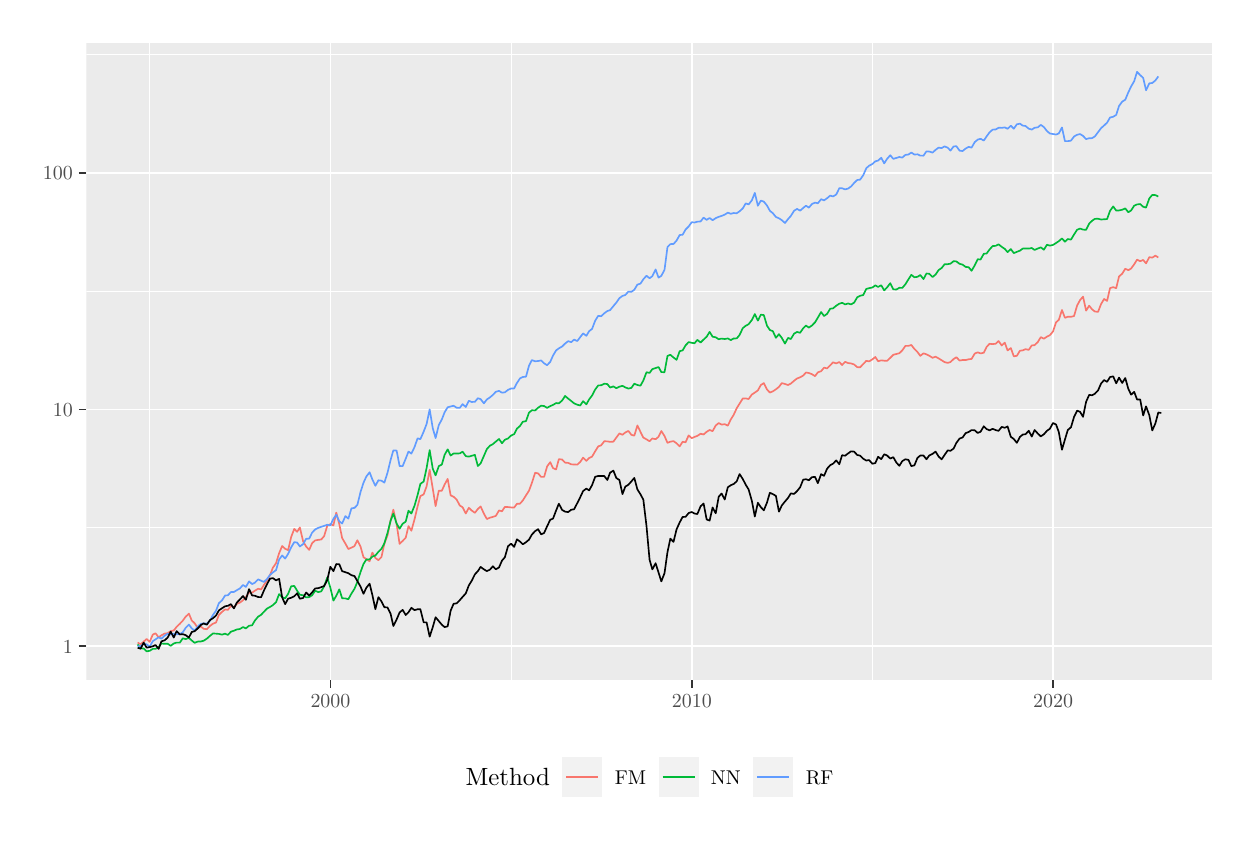
\begin{tikzpicture}[x=1pt,y=1pt]
\definecolor{fillColor}{RGB}{255,255,255}
\path[use as bounding box,fill=fillColor,fill opacity=0.00] (0,0) rectangle (433.62,289.08);
\begin{scope}
\path[clip] (  0.00,  0.00) rectangle (433.62,289.08);
\definecolor{drawColor}{RGB}{255,255,255}
\definecolor{fillColor}{RGB}{255,255,255}

\path[draw=drawColor,line width= 0.6pt,line join=round,line cap=round,fill=fillColor] (  0.00,  0.00) rectangle (433.62,289.08);
\end{scope}
\begin{scope}
\path[clip] ( 21.25, 53.26) rectangle (428.12,283.58);
\definecolor{fillColor}{gray}{0.92}

\path[fill=fillColor] ( 21.25, 53.26) rectangle (428.12,283.58);
\definecolor{drawColor}{RGB}{255,255,255}

\path[draw=drawColor,line width= 0.3pt,line join=round] ( 21.25,108.33) --
	(428.12,108.33);

\path[draw=drawColor,line width= 0.3pt,line join=round] ( 21.25,193.89) --
	(428.12,193.89);

\path[draw=drawColor,line width= 0.3pt,line join=round] ( 21.25,279.46) --
	(428.12,279.46);

\path[draw=drawColor,line width= 0.3pt,line join=round] ( 44.12, 53.26) --
	( 44.12,283.58);

\path[draw=drawColor,line width= 0.3pt,line join=round] (174.69, 53.26) --
	(174.69,283.58);

\path[draw=drawColor,line width= 0.3pt,line join=round] (305.25, 53.26) --
	(305.25,283.58);

\path[draw=drawColor,line width= 0.6pt,line join=round] ( 21.25, 65.55) --
	(428.12, 65.55);

\path[draw=drawColor,line width= 0.6pt,line join=round] ( 21.25,151.11) --
	(428.12,151.11);

\path[draw=drawColor,line width= 0.6pt,line join=round] ( 21.25,236.67) --
	(428.12,236.67);

\path[draw=drawColor,line width= 0.6pt,line join=round] (109.41, 53.26) --
	(109.41,283.58);

\path[draw=drawColor,line width= 0.6pt,line join=round] (239.98, 53.26) --
	(239.98,283.58);

\path[draw=drawColor,line width= 0.6pt,line join=round] (370.52, 53.26) --
	(370.52,283.58);
\definecolor{drawColor}{RGB}{248,118,109}

\path[draw=drawColor,line width= 0.6pt,line join=round] ( 39.74, 66.92) --
	( 40.81, 66.24) --
	( 41.92, 67.23) --
	( 42.99, 68.18) --
	( 44.07, 67.13) --
	( 45.21, 69.78) --
	( 46.21, 70.23) --
	( 47.32, 68.79) --
	( 48.32, 69.51) --
	( 49.50, 70.14) --
	( 50.57, 70.26) --
	( 51.68, 71.05) --
	( 52.79, 71.26) --
	( 53.82, 72.57) --
	( 54.97, 73.67) --
	( 56.04, 74.79) --
	( 57.08, 76.22) --
	( 58.26, 77.34) --
	( 59.29, 74.86) --
	( 60.33, 73.88) --
	( 61.47, 72.15) --
	( 62.58, 72.68) --
	( 63.58, 71.86) --
	( 64.76, 71.72) --
	( 65.84, 72.87) --
	( 66.94, 73.70) --
	( 68.05, 74.12) --
	( 69.09, 76.87) --
	( 70.23, 77.97) --
	( 71.34, 78.87) --
	( 72.34, 78.69) --
	( 73.45, 80.15) --
	( 74.52, 79.49) --
	( 75.59, 80.90) --
	( 76.70, 81.32) --
	( 77.81, 82.17) --
	( 78.85, 83.34) --
	( 79.99, 84.99) --
	( 81.10, 84.93) --
	( 82.10, 85.62) --
	( 83.28, 86.34) --
	( 84.35, 86.07) --
	( 85.35, 87.67) --
	( 86.50, 89.37) --
	( 87.57, 91.30) --
	( 88.60, 93.91) --
	( 89.75, 95.59) --
	( 90.86, 99.18) --
	( 91.96,101.78) --
	( 93.04,100.77) --
	( 94.11,100.29) --
	( 95.22,105.05) --
	( 96.33,107.97) --
	( 97.36,106.90) --
	( 98.36,108.48) --
	( 99.54,103.43) --
	(100.61,101.62) --
	(101.72,100.38) --
	(102.79,102.82) --
	(103.87,103.80) --
	(105.01,104.00) --
	(106.08,104.14) --
	(107.12,105.34) --
	(108.26,109.11) --
	(109.37,109.66) --
	(110.48,109.26) --
	(111.52,113.84) --
	(112.62,109.59) --
	(113.63,104.65) --
	(114.81,102.65) --
	(115.88,100.69) --
	(116.99,101.19) --
	(118.09,101.75) --
	(119.13,103.86) --
	(120.27,101.59) --
	(121.35, 97.72) --
	(122.38, 97.06) --
	(123.56, 96.27) --
	(124.56, 99.40) --
	(125.64, 97.45) --
	(126.74, 96.66) --
	(127.85, 97.83) --
	(128.89,102.63) --
	(130.03,105.61) --
	(131.14,111.05) --
	(132.14,114.92) --
	(133.32,109.68) --
	(134.39,102.55) --
	(135.50,103.61) --
	(136.61,104.78) --
	(137.61,108.97) --
	(138.65,107.31) --
	(139.79,111.44) --
	(140.90,116.10) --
	(141.90,119.82) --
	(143.08,120.43) --
	(144.15,123.33) --
	(145.26,129.32) --
	(146.37,122.56) --
	(147.40,116.19) --
	(148.55,121.77) --
	(149.66,121.77) --
	(150.66,123.99) --
	(151.76,126.03) --
	(152.84,120.06) --
	(153.91,119.58) --
	(155.02,118.55) --
	(156.13,116.42) --
	(157.16,115.78) --
	(158.31,113.54) --
	(159.41,115.59) --
	(160.42,114.63) --
	(161.59,113.76) --
	(162.67,115.15) --
	(163.67,116.08) --
	(164.85,113.48) --
	(165.92,111.53) --
	(167.03,112.01) --
	(168.10,112.29) --
	(169.17,112.67) --
	(170.32,114.63) --
	(171.39,114.32) --
	(172.43,115.92) --
	(173.57,115.85) --
	(174.68,115.72) --
	(175.79,115.67) --
	(176.79,117.03) --
	(177.89,117.08) --
	(178.93,118.25) --
	(180.07,120.09) --
	(181.15,121.76) --
	(182.18,124.52) --
	(183.36,128.24) --
	(184.44,128.02) --
	(185.54,126.75) --
	(186.62,126.78) --
	(187.69,130.53) --
	(188.83,132.07) --
	(189.83,129.92) --
	(190.94,129.43) --
	(191.94,133.15) --
	(193.12,133.03) --
	(194.19,131.90) --
	(195.30,131.81) --
	(196.41,131.30) --
	(197.45,131.22) --
	(198.59,131.19) --
	(199.66,132.14) --
	(200.70,133.70) --
	(201.88,132.54) --
	(202.88,133.58) --
	(203.95,134.09) --
	(205.06,136.00) --
	(206.17,137.78) --
	(207.20,138.15) --
	(208.35,139.62) --
	(209.46,139.59) --
	(210.46,139.41) --
	(211.64,139.49) --
	(212.71,140.97) --
	(213.82,142.46) --
	(214.93,141.97) --
	(215.96,142.81) --
	(217.07,143.35) --
	(218.14,141.96) --
	(219.21,141.65) --
	(220.32,145.35) --
	(221.43,143.03) --
	(222.47,140.95) --
	(223.61,140.32) --
	(224.72,139.63) --
	(225.72,140.64) --
	(226.90,140.37) --
	(227.97,141.26) --
	(228.97,143.33) --
	(230.12,141.53) --
	(231.19,139.05) --
	(232.23,139.47) --
	(233.37,139.68) --
	(234.48,138.89) --
	(235.59,137.77) --
	(236.66,139.45) --
	(237.73,139.25) --
	(238.84,141.75) --
	(239.95,140.74) --
	(240.98,141.20) --
	(241.98,141.58) --
	(243.16,142.34) --
	(244.24,142.08) --
	(245.34,143.04) --
	(246.42,143.71) --
	(247.49,143.28) --
	(248.63,145.34) --
	(249.70,146.20) --
	(250.74,145.65) --
	(251.89,145.79) --
	(252.99,145.28) --
	(254.10,147.56) --
	(255.10,149.16) --
	(256.21,151.56) --
	(257.25,153.24) --
	(258.39,155.07) --
	(259.46,155.12) --
	(260.50,154.88) --
	(261.68,156.52) --
	(262.75,157.21) --
	(263.86,158.01) --
	(264.93,159.95) --
	(266.00,160.66) --
	(267.15,158.34) --
	(268.18,157.23) --
	(269.26,157.66) --
	(270.37,158.40) --
	(271.47,159.27) --
	(272.51,160.64) --
	(273.65,160.33) --
	(274.76,159.95) --
	(275.76,160.47) --
	(276.94,161.49) --
	(278.01,162.31) --
	(279.12,162.74) --
	(280.23,163.37) --
	(281.23,164.47) --
	(282.27,164.30) --
	(283.41,163.85) --
	(284.52,163.16) --
	(285.52,164.52) --
	(286.70,164.95) --
	(287.77,166.23) --
	(288.88,165.95) --
	(289.99,167.08) --
	(291.03,168.16) --
	(292.17,167.76) --
	(293.28,168.26) --
	(294.28,167.18) --
	(295.39,168.33) --
	(296.46,167.88) --
	(297.53,167.76) --
	(298.64,167.37) --
	(299.75,166.41) --
	(300.78,166.33) --
	(301.93,167.55) --
	(303.04,168.69) --
	(304.04,168.48) --
	(305.22,169.22) --
	(306.29,170.08) --
	(307.29,168.54) --
	(308.43,168.87) --
	(309.51,168.74) --
	(310.54,168.69) --
	(311.69,169.77) --
	(312.79,170.88) --
	(313.90,171.16) --
	(314.97,171.44) --
	(316.05,172.48) --
	(317.15,174.08) --
	(318.26,174.09) --
	(319.30,174.43) --
	(320.41,172.98) --
	(321.52,171.87) --
	(322.55,170.48) --
	(323.70,171.41) --
	(324.77,171.04) --
	(325.80,170.51) --
	(326.98,169.79) --
	(328.06,170.19) --
	(329.16,169.58) --
	(330.24,168.91) --
	(331.31,168.23) --
	(332.45,167.94) --
	(333.45,168.27) --
	(334.56,169.32) --
	(335.56,170.00) --
	(336.74,168.80) --
	(337.82,168.98) --
	(338.92,168.96) --
	(340.03,169.25) --
	(341.07,169.38) --
	(342.21,171.31) --
	(343.28,171.77) --
	(344.32,171.37) --
	(345.50,171.62) --
	(346.50,173.71) --
	(347.57,174.85) --
	(348.68,174.73) --
	(349.79,174.87) --
	(350.83,175.83) --
	(351.97,174.24) --
	(353.08,175.26) --
	(354.08,172.44) --
	(355.26,173.31) --
	(356.33,170.32) --
	(357.44,170.50) --
	(358.55,172.35) --
	(359.55,172.47) --
	(360.58,172.91) --
	(361.73,172.65) --
	(362.84,174.27) --
	(363.84,174.35) --
	(365.02,175.49) --
	(366.09,177.26) --
	(367.20,176.67) --
	(368.31,177.43) --
	(369.34,177.92) --
	(370.49,179.28) --
	(371.59,182.60) --
	(372.59,183.49) --
	(373.74,187.05) --
	(374.81,184.24) --
	(375.85,184.62) --
	(376.99,184.59) --
	(378.10,184.87) --
	(379.21,188.67) --
	(380.28,190.65) --
	(381.35,191.89) --
	(382.46,186.83) --
	(383.57,188.62) --
	(384.60,187.31) --
	(385.61,186.51) --
	(386.79,186.40) --
	(387.86,189.20) --
	(388.97,191.04) --
	(390.04,190.32) --
	(391.11,194.96) --
	(392.25,195.32) --
	(393.33,194.93) --
	(394.36,199.18) --
	(395.51,200.18) --
	(396.61,201.97) --
	(397.72,201.44) --
	(398.72,202.05) --
	(399.83,203.57) --
	(400.87,205.24) --
	(402.01,204.68) --
	(403.08,205.15) --
	(404.12,203.91) --
	(405.30,206.15) --
	(406.37,205.98) --
	(407.48,206.69) --
	(408.55,206.06);
\definecolor{drawColor}{RGB}{0,186,56}

\path[draw=drawColor,line width= 0.6pt,line join=round] ( 39.74, 66.21) --
	( 40.81, 64.80) --
	( 41.92, 64.74) --
	( 42.99, 63.73) --
	( 44.07, 63.91) --
	( 45.21, 64.60) --
	( 46.21, 64.60) --
	( 47.32, 65.21) --
	( 48.32, 66.56) --
	( 49.50, 66.43) --
	( 50.57, 66.48) --
	( 51.68, 65.71) --
	( 52.79, 66.56) --
	( 53.82, 66.88) --
	( 54.97, 66.85) --
	( 56.04, 68.43) --
	( 57.08, 68.14) --
	( 58.26, 68.56) --
	( 59.29, 67.64) --
	( 60.33, 66.80) --
	( 61.47, 67.24) --
	( 62.58, 67.29) --
	( 63.58, 67.54) --
	( 64.76, 68.31) --
	( 65.84, 69.28) --
	( 66.94, 70.17) --
	( 68.05, 70.11) --
	( 69.09, 70.01) --
	( 70.23, 69.75) --
	( 71.34, 70.11) --
	( 72.34, 69.64) --
	( 73.45, 70.83) --
	( 74.52, 71.17) --
	( 75.59, 71.62) --
	( 76.70, 71.79) --
	( 77.81, 72.49) --
	( 78.85, 72.01) --
	( 79.99, 72.97) --
	( 81.10, 73.13) --
	( 82.10, 74.83) --
	( 83.28, 76.26) --
	( 84.35, 76.91) --
	( 85.35, 77.99) --
	( 86.50, 79.18) --
	( 87.57, 79.75) --
	( 88.60, 80.42) --
	( 89.75, 81.48) --
	( 90.86, 84.41) --
	( 91.96, 83.28) --
	( 93.04, 82.88) --
	( 94.11, 84.50) --
	( 95.22, 87.22) --
	( 96.33, 87.35) --
	( 97.36, 85.63) --
	( 98.36, 84.15) --
	( 99.54, 84.00) --
	(100.61, 83.21) --
	(101.72, 83.31) --
	(102.79, 83.98) --
	(103.87, 85.63) --
	(105.01, 85.11) --
	(106.08, 85.39) --
	(107.12, 87.22) --
	(108.26, 90.43) --
	(109.37, 86.73) --
	(110.48, 82.04) --
	(111.52, 83.82) --
	(112.62, 86.12) --
	(113.63, 82.90) --
	(114.81, 82.84) --
	(115.88, 82.55) --
	(116.99, 84.59) --
	(118.09, 86.30) --
	(119.13, 88.80) --
	(120.27, 92.36) --
	(121.35, 95.30) --
	(122.38, 96.90) --
	(123.56, 96.95) --
	(124.56, 97.97) --
	(125.64, 98.33) --
	(126.74, 99.70) --
	(127.85,100.76) --
	(128.89,102.79) --
	(130.03,106.51) --
	(131.14,110.90) --
	(132.14,113.50) --
	(133.32,109.88) --
	(134.39,108.04) --
	(135.50,109.83) --
	(136.61,110.60) --
	(137.61,114.54) --
	(138.65,113.52) --
	(139.79,116.36) --
	(140.90,120.23) --
	(141.90,124.23) --
	(143.08,125.07) --
	(144.15,129.94) --
	(145.26,136.44) --
	(146.37,129.72) --
	(147.40,127.30) --
	(148.55,130.63) --
	(149.66,131.22) --
	(150.66,134.73) --
	(151.76,136.70) --
	(152.84,134.47) --
	(153.91,135.21) --
	(155.02,135.22) --
	(156.13,135.24) --
	(157.16,135.86) --
	(158.31,134.25) --
	(159.41,134.07) --
	(160.42,134.37) --
	(161.59,134.70) --
	(162.67,130.69) --
	(163.67,131.61) --
	(164.85,134.32) --
	(165.92,136.80) --
	(167.03,138.02) --
	(168.10,138.60) --
	(169.17,139.52) --
	(170.32,140.45) --
	(171.39,138.90) --
	(172.43,140.18) --
	(173.57,140.63) --
	(174.68,141.70) --
	(175.79,142.21) --
	(176.79,144.18) --
	(177.89,145.15) --
	(178.93,146.69) --
	(180.07,146.90) --
	(181.15,149.97) --
	(182.18,150.83) --
	(183.36,150.76) --
	(184.44,151.75) --
	(185.54,152.48) --
	(186.62,152.35) --
	(187.69,151.71) --
	(188.83,152.34) --
	(189.83,152.76) --
	(190.94,153.43) --
	(191.94,153.31) --
	(193.12,154.36) --
	(194.19,155.99) --
	(195.30,155.05) --
	(196.41,154.18) --
	(197.45,153.33) --
	(198.59,152.84) --
	(199.66,152.55) --
	(200.70,154.11) --
	(201.88,152.97) --
	(202.88,154.76) --
	(203.95,156.17) --
	(205.06,158.31) --
	(206.17,159.81) --
	(207.20,159.85) --
	(208.35,160.42) --
	(209.46,160.30) --
	(210.46,159.04) --
	(211.64,159.45) --
	(212.71,158.80) --
	(213.82,159.34) --
	(214.93,159.66) --
	(215.96,159.09) --
	(217.07,158.67) --
	(218.14,158.92) --
	(219.21,160.42) --
	(220.32,159.96) --
	(221.43,159.71) --
	(222.47,161.58) --
	(223.61,164.57) --
	(224.72,164.32) --
	(225.72,165.70) --
	(226.90,166.07) --
	(227.97,166.45) --
	(228.97,164.61) --
	(230.12,164.58) --
	(231.19,170.47) --
	(232.23,170.87) --
	(233.37,169.89) --
	(234.48,169.06) --
	(235.59,172.17) --
	(236.66,172.46) --
	(237.73,174.28) --
	(238.84,175.46) --
	(239.95,175.20) --
	(240.98,175.05) --
	(241.98,176.27) --
	(243.16,175.31) --
	(244.24,176.37) --
	(245.34,177.39) --
	(246.42,179.15) --
	(247.49,177.41) --
	(248.63,177.18) --
	(249.70,176.49) --
	(250.74,176.73) --
	(251.89,176.57) --
	(252.99,176.78) --
	(254.10,176.20) --
	(255.10,176.77) --
	(256.21,176.80) --
	(257.25,178.04) --
	(258.39,180.49) --
	(259.46,181.36) --
	(260.50,181.92) --
	(261.68,183.44) --
	(262.75,185.60) --
	(263.86,183.22) --
	(264.93,185.37) --
	(266.00,185.23) --
	(267.15,181.40) --
	(268.18,179.83) --
	(269.26,179.41) --
	(270.37,177.01) --
	(271.47,178.32) --
	(272.51,176.96) --
	(273.65,174.92) --
	(274.76,176.98) --
	(275.76,176.56) --
	(276.94,178.51) --
	(278.01,179.13) --
	(279.12,178.82) --
	(280.23,180.47) --
	(281.23,181.42) --
	(282.27,180.71) --
	(283.41,181.48) --
	(284.52,182.60) --
	(285.52,184.29) --
	(286.70,186.33) --
	(287.77,184.87) --
	(288.88,185.68) --
	(289.99,187.52) --
	(291.03,187.65) --
	(292.17,188.62) --
	(293.28,189.33) --
	(294.28,189.66) --
	(295.39,189.08) --
	(296.46,189.42) --
	(297.53,189.09) --
	(298.64,189.73) --
	(299.75,191.64) --
	(300.78,192.20) --
	(301.93,192.46) --
	(303.04,194.66) --
	(304.04,194.96) --
	(305.22,195.18) --
	(306.29,195.95) --
	(307.29,195.40) --
	(308.43,195.99) --
	(309.51,194.15) --
	(310.54,195.21) --
	(311.69,196.75) --
	(312.79,194.54) --
	(313.90,194.46) --
	(314.97,195.08) --
	(316.05,195.05) --
	(317.15,196.35) --
	(318.26,198.13) --
	(319.30,199.76) --
	(320.41,198.90) --
	(321.52,199.04) --
	(322.55,199.70) --
	(323.70,198.23) --
	(324.77,200.24) --
	(325.80,200.15) --
	(326.98,198.97) --
	(328.06,199.87) --
	(329.16,201.48) --
	(330.24,202.21) --
	(331.31,203.57) --
	(332.45,203.62) --
	(333.45,203.80) --
	(334.56,204.69) --
	(335.56,204.62) --
	(336.74,203.74) --
	(337.82,203.46) --
	(338.92,202.63) --
	(340.03,202.52) --
	(341.07,201.24) --
	(342.21,203.17) --
	(343.28,205.39) --
	(344.32,205.31) --
	(345.50,207.39) --
	(346.50,207.46) --
	(347.57,208.92) --
	(348.68,210.16) --
	(349.79,210.24) --
	(350.83,210.78) --
	(351.97,209.89) --
	(353.08,209.13) --
	(354.08,207.98) --
	(355.26,209.07) --
	(356.33,207.62) --
	(357.44,208.07) --
	(358.55,208.51) --
	(359.55,209.25) --
	(360.58,209.31) --
	(361.73,209.25) --
	(362.84,209.45) --
	(363.84,208.76) --
	(365.02,209.28) --
	(366.09,209.69) --
	(367.20,208.85) --
	(368.31,210.63) --
	(369.34,210.33) --
	(370.49,210.56) --
	(371.59,211.25) --
	(372.59,211.91) --
	(373.74,212.93) --
	(374.81,211.74) --
	(375.85,212.70) --
	(376.99,212.49) --
	(378.10,214.34) --
	(379.21,216.05) --
	(380.28,216.49) --
	(381.35,216.11) --
	(382.46,216.03) --
	(383.57,218.29) --
	(384.60,219.28) --
	(385.61,219.99) --
	(386.79,220.03) --
	(387.86,219.75) --
	(388.97,219.84) --
	(390.04,219.92) --
	(391.11,222.90) --
	(392.25,224.48) --
	(393.33,222.99) --
	(394.36,223.04) --
	(395.51,223.29) --
	(396.61,223.77) --
	(397.72,222.39) --
	(398.72,223.02) --
	(399.83,224.75) --
	(400.87,225.21) --
	(402.01,225.34) --
	(403.08,224.36) --
	(404.12,224.07) --
	(405.30,227.38) --
	(406.37,228.65) --
	(407.48,228.58) --
	(408.55,228.04);
\definecolor{drawColor}{RGB}{97,156,255}

\path[draw=drawColor,line width= 0.6pt,line join=round] ( 39.74, 65.55) --
	( 40.81, 65.58) --
	( 41.92, 66.42) --
	( 42.99, 66.24) --
	( 44.07, 65.41) --
	( 45.21, 67.38) --
	( 46.21, 68.07) --
	( 47.32, 68.77) --
	( 48.32, 68.30) --
	( 49.50, 69.37) --
	( 50.57, 70.08) --
	( 51.68, 69.80) --
	( 52.79, 70.08) --
	( 53.82, 69.86) --
	( 54.97, 69.99) --
	( 56.04, 70.57) --
	( 57.08, 72.19) --
	( 58.26, 73.39) --
	( 59.29, 72.01) --
	( 60.33, 71.27) --
	( 61.47, 72.71) --
	( 62.58, 73.69) --
	( 63.58, 73.79) --
	( 64.76, 73.78) --
	( 65.84, 74.76) --
	( 66.94, 76.83) --
	( 68.05, 78.38) --
	( 69.09, 81.12) --
	( 70.23, 82.14) --
	( 71.34, 83.90) --
	( 72.34, 83.97) --
	( 73.45, 85.14) --
	( 74.52, 85.16) --
	( 75.59, 85.83) --
	( 76.70, 86.45) --
	( 77.81, 87.71) --
	( 78.85, 86.99) --
	( 79.99, 88.99) --
	( 81.10, 88.02) --
	( 82.10, 88.52) --
	( 83.28, 89.72) --
	( 84.35, 89.26) --
	( 85.35, 88.79) --
	( 86.50, 89.88) --
	( 87.57, 91.31) --
	( 88.60, 92.23) --
	( 89.75, 93.06) --
	( 90.86, 96.89) --
	( 91.96, 98.37) --
	( 93.04, 97.24) --
	( 94.11, 98.94) --
	( 95.22,101.31) --
	( 96.33,103.18) --
	( 97.36,103.03) --
	( 98.36,101.61) --
	( 99.54,102.48) --
	(100.61,104.37) --
	(101.72,104.45) --
	(102.79,106.63) --
	(103.87,107.75) --
	(105.01,108.32) --
	(106.08,108.73) --
	(107.12,109.04) --
	(108.26,109.46) --
	(109.37,109.22) --
	(110.48,111.62) --
	(111.52,113.06) --
	(112.62,110.67) --
	(113.63,109.91) --
	(114.81,112.59) --
	(115.88,111.67) --
	(116.99,115.38) --
	(118.09,115.55) --
	(119.13,116.62) --
	(120.27,121.27) --
	(121.35,124.64) --
	(122.38,126.91) --
	(123.56,128.41) --
	(124.56,125.81) --
	(125.64,123.54) --
	(126.74,125.53) --
	(127.85,125.38) --
	(128.89,124.68) --
	(130.03,128.27) --
	(131.14,132.86) --
	(132.14,136.35) --
	(133.32,136.25) --
	(134.39,130.68) --
	(135.50,130.64) --
	(136.61,133.37) --
	(137.61,135.91) --
	(138.65,135.16) --
	(139.79,137.55) --
	(140.90,140.69) --
	(141.90,140.39) --
	(143.08,143.09) --
	(144.15,145.86) --
	(145.26,151.15) --
	(146.37,144.38) --
	(147.40,140.79) --
	(148.55,145.46) --
	(149.66,147.53) --
	(150.66,150.09) --
	(151.76,151.91) --
	(152.84,152.20) --
	(153.91,152.46) --
	(155.02,151.73) --
	(156.13,151.69) --
	(157.16,153.03) --
	(158.31,152.01) --
	(159.41,154.26) --
	(160.42,153.83) --
	(161.59,153.87) --
	(162.67,155.17) --
	(163.67,154.85) --
	(164.85,153.34) --
	(165.92,154.72) --
	(167.03,155.47) --
	(168.10,156.39) --
	(169.17,157.51) --
	(170.32,157.83) --
	(171.39,157.18) --
	(172.43,157.31) --
	(173.57,158.19) --
	(174.68,158.71) --
	(175.79,158.72) --
	(176.79,160.68) --
	(177.89,162.34) --
	(178.93,162.85) --
	(180.07,162.97) --
	(181.15,166.92) --
	(182.18,168.95) --
	(183.36,168.53) --
	(184.44,168.62) --
	(185.54,168.83) --
	(186.62,167.79) --
	(187.69,167.12) --
	(188.83,168.33) --
	(189.83,170.59) --
	(190.94,172.46) --
	(191.94,173.20) --
	(193.12,173.87) --
	(194.19,174.93) --
	(195.30,175.79) --
	(196.41,175.45) --
	(197.45,176.36) --
	(198.59,175.84) --
	(199.66,177.25) --
	(200.70,178.60) --
	(201.88,177.74) --
	(202.88,179.41) --
	(203.95,180.24) --
	(205.06,183.19) --
	(206.17,184.96) --
	(207.20,184.80) --
	(208.35,185.86) --
	(209.46,186.69) --
	(210.46,187.02) --
	(211.64,188.46) --
	(212.71,189.73) --
	(213.82,191.34) --
	(214.93,192.15) --
	(215.96,192.50) --
	(217.07,193.71) --
	(218.14,193.62) --
	(219.21,194.38) --
	(220.32,196.23) --
	(221.43,196.59) --
	(222.47,198.17) --
	(223.61,199.43) --
	(224.72,198.54) --
	(225.72,199.27) --
	(226.90,201.71) --
	(227.97,198.73) --
	(228.97,199.41) --
	(230.12,201.58) --
	(231.19,209.80) --
	(232.23,210.87) --
	(233.37,210.91) --
	(234.48,212.16) --
	(235.59,214.14) --
	(236.66,214.25) --
	(237.73,216.14) --
	(238.84,217.24) --
	(239.95,218.78) --
	(240.98,218.68) --
	(241.98,218.97) --
	(243.16,219.05) --
	(244.24,220.44) --
	(245.34,219.63) --
	(246.42,220.32) --
	(247.49,219.51) --
	(248.63,220.26) --
	(249.70,220.72) --
	(250.74,221.05) --
	(251.89,221.53) --
	(252.99,222.22) --
	(254.10,221.83) --
	(255.10,222.10) --
	(256.21,222.02) --
	(257.25,222.74) --
	(258.39,223.76) --
	(259.46,225.59) --
	(260.50,225.21) --
	(261.68,226.68) --
	(262.75,229.39) --
	(263.86,224.74) --
	(264.93,226.59) --
	(266.00,226.21) --
	(267.15,224.82) --
	(268.18,222.93) --
	(269.26,222.04) --
	(270.37,220.68) --
	(271.47,220.20) --
	(272.51,219.51) --
	(273.65,218.51) --
	(274.76,219.91) --
	(275.76,221.04) --
	(276.94,222.92) --
	(278.01,223.58) --
	(279.12,222.96) --
	(280.23,223.92) --
	(281.23,224.75) --
	(282.27,224.04) --
	(283.41,225.36) --
	(284.52,225.87) --
	(285.52,225.62) --
	(286.70,227.09) --
	(287.77,226.68) --
	(288.88,227.45) --
	(289.99,228.40) --
	(291.03,228.09) --
	(292.17,228.79) --
	(293.28,231.06) --
	(294.28,231.05) --
	(295.39,230.63) --
	(296.46,230.95) --
	(297.53,231.68) --
	(298.64,232.98) --
	(299.75,234.04) --
	(300.78,234.14) --
	(301.93,235.77) --
	(303.04,238.31) --
	(304.04,239.18) --
	(305.22,239.81) --
	(306.29,240.78) --
	(307.29,241.05) --
	(308.43,242.07) --
	(309.51,240.04) --
	(310.54,241.67) --
	(311.69,242.98) --
	(312.79,241.67) --
	(313.90,242.01) --
	(314.97,242.35) --
	(316.05,242.14) --
	(317.15,243.10) --
	(318.26,243.24) --
	(319.30,243.96) --
	(320.41,243.23) --
	(321.52,243.32) --
	(322.55,242.85) --
	(323.70,242.82) --
	(324.77,244.39) --
	(325.80,244.31) --
	(326.98,243.94) --
	(328.06,244.92) --
	(329.16,245.73) --
	(330.24,245.56) --
	(331.31,246.18) --
	(332.45,245.71) --
	(333.45,244.65) --
	(334.56,246.12) --
	(335.56,246.27) --
	(336.74,244.64) --
	(337.82,244.50) --
	(338.92,245.39) --
	(340.03,246.02) --
	(341.07,245.73) --
	(342.21,247.71) --
	(343.28,248.62) --
	(344.32,248.92) --
	(345.50,248.30) --
	(346.50,249.79) --
	(347.57,251.25) --
	(348.68,252.23) --
	(349.79,252.29) --
	(350.83,252.90) --
	(351.97,252.88) --
	(353.08,253.03) --
	(354.08,252.54) --
	(355.26,253.64) --
	(356.33,252.57) --
	(357.44,254.17) --
	(358.55,254.38) --
	(359.55,253.70) --
	(360.58,253.54) --
	(361.73,252.58) --
	(362.84,252.26) --
	(363.84,252.91) --
	(365.02,253.08) --
	(366.09,253.94) --
	(367.20,253.17) --
	(368.31,251.73) --
	(369.34,250.85) --
	(370.49,250.65) --
	(371.59,250.46) --
	(372.59,250.85) --
	(373.74,253.02) --
	(374.81,248.07) --
	(375.85,248.08) --
	(376.99,248.25) --
	(378.10,249.75) --
	(379.21,250.38) --
	(380.28,250.64) --
	(381.35,249.97) --
	(382.46,248.80) --
	(383.57,249.14) --
	(384.60,249.15) --
	(385.61,249.77) --
	(386.79,251.32) --
	(387.86,252.75) --
	(388.97,253.75) --
	(390.04,254.75) --
	(391.11,256.61) --
	(392.25,256.89) --
	(393.33,257.55) --
	(394.36,260.79) --
	(395.51,262.36) --
	(396.61,263.04) --
	(397.72,265.72) --
	(398.72,267.82) --
	(399.83,269.74) --
	(400.87,273.11) --
	(402.01,271.92) --
	(403.08,270.93) --
	(404.12,266.47) --
	(405.30,268.96) --
	(406.37,269.09) --
	(407.48,269.99) --
	(408.55,271.46);
\definecolor{drawColor}{RGB}{0,0,0}

\path[draw=drawColor,line width= 0.6pt,line join=round] ( 39.74, 65.03) --
	( 40.81, 64.65) --
	( 41.92, 66.86) --
	( 42.99, 65.04) --
	( 44.07, 65.24) --
	( 45.21, 65.55) --
	( 46.21, 65.99) --
	( 47.32, 64.60) --
	( 48.32, 67.32) --
	( 49.50, 67.71) --
	( 50.57, 68.67) --
	( 51.68, 70.84) --
	( 52.79, 68.70) --
	( 53.82, 71.03) --
	( 54.97, 69.82) --
	( 56.04, 69.91) --
	( 57.08, 69.57) --
	( 58.26, 68.70) --
	( 59.29, 70.73) --
	( 60.33, 71.00) --
	( 61.47, 72.01) --
	( 62.58, 73.22) --
	( 63.58, 73.80) --
	( 64.76, 73.34) --
	( 65.84, 74.98) --
	( 66.94, 75.68) --
	( 68.05, 76.64) --
	( 69.09, 78.49) --
	( 70.23, 79.30) --
	( 71.34, 80.01) --
	( 72.34, 80.18) --
	( 73.45, 80.77) --
	( 74.52, 79.23) --
	( 75.59, 81.34) --
	( 76.70, 82.49) --
	( 77.81, 83.69) --
	( 78.85, 82.36) --
	( 79.99, 86.19) --
	( 81.10, 83.93) --
	( 82.10, 83.81) --
	( 83.28, 83.34) --
	( 84.35, 83.28) --
	( 85.35, 85.65) --
	( 86.50, 88.04) --
	( 87.57, 89.98) --
	( 88.60, 90.18) --
	( 89.75, 89.37) --
	( 90.86, 89.90) --
	( 91.96, 83.21) --
	( 93.04, 80.77) --
	( 94.11, 82.75) --
	( 95.22, 83.08) --
	( 96.33, 83.62) --
	( 97.36, 84.69) --
	( 98.36, 82.73) --
	( 99.54, 83.00) --
	(100.61, 84.97) --
	(101.72, 83.87) --
	(102.79, 85.02) --
	(103.87, 86.43) --
	(105.01, 86.56) --
	(106.08, 86.92) --
	(107.12, 87.31) --
	(108.26, 89.48) --
	(109.37, 94.28) --
	(110.48, 92.70) --
	(111.52, 95.26) --
	(112.62, 95.17) --
	(113.63, 92.68) --
	(114.81, 92.32) --
	(115.88, 91.95) --
	(116.99, 91.23) --
	(118.09, 90.92) --
	(119.13, 89.11) --
	(120.27, 87.13) --
	(121.35, 84.50) --
	(122.38, 86.70) --
	(123.56, 88.16) --
	(124.56, 84.05) --
	(125.64, 78.94) --
	(126.74, 83.29) --
	(127.85, 81.76) --
	(128.89, 79.66) --
	(130.03, 79.57) --
	(131.14, 77.31) --
	(132.14, 72.86) --
	(133.32, 75.24) --
	(134.39, 77.75) --
	(135.50, 78.70) --
	(136.61, 76.84) --
	(137.61, 77.84) --
	(138.65, 79.45) --
	(139.79, 78.60) --
	(140.90, 78.93) --
	(141.90, 78.95) --
	(143.08, 74.21) --
	(144.15, 74.16) --
	(145.26, 69.02) --
	(146.37, 72.43) --
	(147.40, 76.04) --
	(148.55, 74.66) --
	(149.66, 73.34) --
	(150.66, 72.47) --
	(151.76, 72.76) --
	(152.84, 78.42) --
	(153.91, 80.91) --
	(155.02, 81.07) --
	(156.13, 82.19) --
	(157.16, 83.39) --
	(158.31, 84.65) --
	(159.41, 87.54) --
	(160.42, 89.17) --
	(161.59, 91.52) --
	(162.67, 92.70) --
	(163.67, 94.22) --
	(164.85, 93.35) --
	(165.92, 92.71) --
	(167.03, 93.24) --
	(168.10, 94.45) --
	(169.17, 93.36) --
	(170.32, 94.03) --
	(171.39, 96.50) --
	(172.43, 97.69) --
	(173.57,101.69) --
	(174.68,102.63) --
	(175.79,101.46) --
	(176.79,104.18) --
	(177.89,103.40) --
	(178.93,102.41) --
	(180.07,103.15) --
	(181.15,104.07) --
	(182.18,105.89) --
	(183.36,107.15) --
	(184.44,107.85) --
	(185.54,105.99) --
	(186.62,106.50) --
	(187.69,108.89) --
	(188.83,111.28) --
	(189.83,111.66) --
	(190.94,114.60) --
	(191.94,117.07) --
	(193.12,114.81) --
	(194.19,114.20) --
	(195.30,114.03) --
	(196.41,114.89) --
	(197.45,115.05) --
	(198.59,117.27) --
	(199.66,119.41) --
	(200.70,121.64) --
	(201.88,122.52) --
	(202.88,121.87) --
	(203.95,123.81) --
	(205.06,126.76) --
	(206.17,127.11) --
	(207.20,127.06) --
	(208.35,127.06) --
	(209.46,125.64) --
	(210.46,128.29) --
	(211.64,129.01) --
	(212.71,126.35) --
	(213.82,125.63) --
	(214.93,120.54) --
	(215.96,123.24) --
	(217.07,123.92) --
	(218.14,125.12) --
	(219.21,126.39) --
	(220.32,122.23) --
	(221.43,120.48) --
	(222.47,118.52) --
	(223.61,108.99) --
	(224.72, 96.83) --
	(225.72, 93.32) --
	(226.90, 95.56) --
	(227.97, 92.17) --
	(228.97, 88.99) --
	(230.12, 91.97) --
	(231.19, 99.58) --
	(232.23,104.44) --
	(233.37,103.27) --
	(234.48,107.82) --
	(235.59,110.28) --
	(236.66,112.28) --
	(237.73,112.31) --
	(238.84,113.69) --
	(239.95,114.06) --
	(240.98,113.52) --
	(241.98,113.32) --
	(243.16,116.13) --
	(244.24,117.15) --
	(245.34,111.37) --
	(246.42,110.96) --
	(247.49,115.68) --
	(248.63,113.60) --
	(249.70,119.58) --
	(250.74,120.74) --
	(251.89,118.58) --
	(252.99,122.99) --
	(254.10,123.76) --
	(255.10,124.18) --
	(256.21,125.15) --
	(257.25,127.77) --
	(258.39,126.01) --
	(259.46,123.93) --
	(260.50,122.23) --
	(261.68,118.10) --
	(262.75,112.43) --
	(263.86,117.39) --
	(264.93,115.81) --
	(266.00,114.66) --
	(267.15,117.48) --
	(268.18,121.02) --
	(269.26,120.54) --
	(270.37,119.89) --
	(271.47,114.19) --
	(272.51,116.44) --
	(273.65,117.86) --
	(274.76,119.15) --
	(275.76,120.80) --
	(276.94,120.59) --
	(278.01,121.62) --
	(279.12,122.99) --
	(280.23,125.76) --
	(281.23,125.90) --
	(282.27,125.54) --
	(283.41,126.66) --
	(284.52,126.74) --
	(285.52,124.49) --
	(286.70,127.73) --
	(287.77,127.14) --
	(288.88,129.74) --
	(289.99,130.98) --
	(291.03,131.54) --
	(292.17,132.72) --
	(293.28,131.33) --
	(294.28,134.59) --
	(295.39,134.41) --
	(296.46,135.24) --
	(297.53,135.99) --
	(298.64,135.88) --
	(299.75,134.67) --
	(300.78,134.44) --
	(301.93,133.30) --
	(303.04,132.66) --
	(304.04,132.84) --
	(305.22,131.51) --
	(306.29,131.73) --
	(307.29,134.02) --
	(308.43,133.17) --
	(309.51,134.93) --
	(310.54,134.49) --
	(311.69,133.38) --
	(312.79,133.88) --
	(313.90,131.93) --
	(314.97,130.75) --
	(316.05,132.47) --
	(317.15,133.12) --
	(318.26,132.90) --
	(319.30,130.65) --
	(320.41,130.92) --
	(321.52,133.62) --
	(322.55,134.47) --
	(323.70,134.46) --
	(324.77,133.12) --
	(325.80,134.50) --
	(326.98,135.07) --
	(328.06,135.90) --
	(329.16,134.13) --
	(330.24,133.09) --
	(331.31,134.66) --
	(332.45,136.34) --
	(333.45,136.18) --
	(334.56,136.97) --
	(335.56,139.01) --
	(336.74,140.61) --
	(337.82,140.99) --
	(338.92,142.55) --
	(340.03,142.99) --
	(341.07,143.66) --
	(342.21,143.61) --
	(343.28,142.62) --
	(344.32,143.08) --
	(345.50,145.05) --
	(346.50,144.05) --
	(347.57,143.57) --
	(348.68,144.13) --
	(349.79,143.66) --
	(350.83,143.40) --
	(351.97,144.82) --
	(353.08,144.50) --
	(354.08,145.00) --
	(355.26,141.23) --
	(356.33,140.45) --
	(357.44,139.06) --
	(358.55,141.19) --
	(359.55,142.04) --
	(360.58,142.18) --
	(361.73,143.42) --
	(362.84,141.32) --
	(363.84,143.70) --
	(365.02,142.41) --
	(366.09,141.39) --
	(367.20,142.14) --
	(368.31,143.41) --
	(369.34,144.11) --
	(370.49,146.21) --
	(371.59,145.71) --
	(372.59,142.96) --
	(373.74,136.57) --
	(374.81,140.24) --
	(375.85,143.71) --
	(376.99,144.68) --
	(378.10,148.41) --
	(379.21,150.69) --
	(380.28,150.26) --
	(381.35,148.46) --
	(382.46,153.90) --
	(383.57,156.38) --
	(384.60,156.25) --
	(385.61,156.79) --
	(386.79,158.02) --
	(387.86,160.48) --
	(388.97,161.74) --
	(390.04,161.11) --
	(391.11,162.83) --
	(392.25,163.09) --
	(393.33,160.56) --
	(394.36,162.62) --
	(395.51,160.70) --
	(396.61,162.48) --
	(397.72,158.56) --
	(398.72,156.46) --
	(399.83,157.49) --
	(400.87,154.72) --
	(402.01,154.70) --
	(403.08,148.95) --
	(404.12,152.24) --
	(405.30,149.03) --
	(406.37,143.54) --
	(407.48,146.04) --
	(408.55,150.02) --
	(409.63,149.84);
\end{scope}
\begin{scope}
\path[clip] (  0.00,  0.00) rectangle (433.62,289.08);
\definecolor{drawColor}{gray}{0.30}

\node[text=drawColor,anchor=base east,inner sep=0pt, outer sep=0pt, scale=  0.72] at ( 16.30, 63.07) {1};

\node[text=drawColor,anchor=base east,inner sep=0pt, outer sep=0pt, scale=  0.72] at ( 16.30,148.63) {10};

\node[text=drawColor,anchor=base east,inner sep=0pt, outer sep=0pt, scale=  0.72] at ( 16.30,234.20) {100};
\end{scope}
\begin{scope}
\path[clip] (  0.00,  0.00) rectangle (433.62,289.08);
\definecolor{drawColor}{gray}{0.20}

\path[draw=drawColor,line width= 0.6pt,line join=round] ( 18.50, 65.55) --
	( 21.25, 65.55);

\path[draw=drawColor,line width= 0.6pt,line join=round] ( 18.50,151.11) --
	( 21.25,151.11);

\path[draw=drawColor,line width= 0.6pt,line join=round] ( 18.50,236.67) --
	( 21.25,236.67);
\end{scope}
\begin{scope}
\path[clip] (  0.00,  0.00) rectangle (433.62,289.08);
\definecolor{drawColor}{gray}{0.20}

\path[draw=drawColor,line width= 0.6pt,line join=round] (109.41, 50.51) --
	(109.41, 53.26);

\path[draw=drawColor,line width= 0.6pt,line join=round] (239.98, 50.51) --
	(239.98, 53.26);

\path[draw=drawColor,line width= 0.6pt,line join=round] (370.52, 50.51) --
	(370.52, 53.26);
\end{scope}
\begin{scope}
\path[clip] (  0.00,  0.00) rectangle (433.62,289.08);
\definecolor{drawColor}{gray}{0.30}

\node[text=drawColor,anchor=base,inner sep=0pt, outer sep=0pt, scale=  0.72] at (109.41, 43.35) {2000};

\node[text=drawColor,anchor=base,inner sep=0pt, outer sep=0pt, scale=  0.72] at (239.98, 43.35) {2010};

\node[text=drawColor,anchor=base,inner sep=0pt, outer sep=0pt, scale=  0.72] at (370.52, 43.35) {2020};
\end{scope}
\begin{scope}
\path[clip] (  0.00,  0.00) rectangle (433.62,289.08);
\definecolor{fillColor}{RGB}{255,255,255}

\path[fill=fillColor] (152.71,  5.50) rectangle (296.66, 30.95);
\end{scope}
\begin{scope}
\path[clip] (  0.00,  0.00) rectangle (433.62,289.08);
\definecolor{drawColor}{RGB}{0,0,0}

\node[text=drawColor,anchor=base west,inner sep=0pt, outer sep=0pt, scale=  0.90] at (158.21, 15.13) {Method};
\end{scope}
\begin{scope}
\path[clip] (  0.00,  0.00) rectangle (433.62,289.08);
\definecolor{fillColor}{gray}{0.95}

\path[fill=fillColor] (193.20, 11.00) rectangle (207.66, 25.45);
\end{scope}
\begin{scope}
\path[clip] (  0.00,  0.00) rectangle (433.62,289.08);
\definecolor{drawColor}{RGB}{248,118,109}

\path[draw=drawColor,line width= 0.6pt,line join=round] (194.65, 18.23) -- (206.21, 18.23);
\end{scope}
\begin{scope}
\path[clip] (  0.00,  0.00) rectangle (433.62,289.08);
\definecolor{fillColor}{gray}{0.95}

\path[fill=fillColor] (227.95, 11.00) rectangle (242.41, 25.45);
\end{scope}
\begin{scope}
\path[clip] (  0.00,  0.00) rectangle (433.62,289.08);
\definecolor{drawColor}{RGB}{0,186,56}

\path[draw=drawColor,line width= 0.6pt,line join=round] (229.40, 18.23) -- (240.96, 18.23);
\end{scope}
\begin{scope}
\path[clip] (  0.00,  0.00) rectangle (433.62,289.08);
\definecolor{fillColor}{gray}{0.95}

\path[fill=fillColor] (262.21, 11.00) rectangle (276.66, 25.45);
\end{scope}
\begin{scope}
\path[clip] (  0.00,  0.00) rectangle (433.62,289.08);
\definecolor{drawColor}{RGB}{97,156,255}

\path[draw=drawColor,line width= 0.6pt,line join=round] (263.65, 18.23) -- (275.21, 18.23);
\end{scope}
\begin{scope}
\path[clip] (  0.00,  0.00) rectangle (433.62,289.08);
\definecolor{drawColor}{RGB}{0,0,0}

\node[text=drawColor,anchor=base west,inner sep=0pt, outer sep=0pt, scale=  0.72] at (212.16, 15.75) {FM};
\end{scope}
\begin{scope}
\path[clip] (  0.00,  0.00) rectangle (433.62,289.08);
\definecolor{drawColor}{RGB}{0,0,0}

\node[text=drawColor,anchor=base west,inner sep=0pt, outer sep=0pt, scale=  0.72] at (246.91, 15.75) {NN};
\end{scope}
\begin{scope}
\path[clip] (  0.00,  0.00) rectangle (433.62,289.08);
\definecolor{drawColor}{RGB}{0,0,0}

\node[text=drawColor,anchor=base west,inner sep=0pt, outer sep=0pt, scale=  0.72] at (281.16, 15.75) {RF};
\end{scope}
\end{tikzpicture}

\label{plot:cumul_ew_LS_portf_return}
\end{figure}

\begin{table}[h]
\small
\caption[Expected return regressions]{\textbf{...} \\ ...}
\label{table:expRetRegressions}
\centering
\newcolumntype{Y}{>{\centering\arraybackslash}X}
\begin{tabularx}{\textwidth}{@{\extracolsep{4pt}} X Y Y Y Y Y Y} 
\toprule
& \multicolumn{2}{c}{Univariate properties} & \multicolumn{4}{c}{Predictive ability}\\
\cline{2-3}\cline{4-7}
& Mean & Std. & Slope. & SE & t-stat & $R^2$ \\
\midrule
FM & 0.0119 & 0.0160 & 0.1593 & 0.0217 & 7.324 & 0.0004 \\
RF & 0.0073 & 0.0117 & 0.4877 & 0.0298 & 16.388 & 0.0022 \\
NN & 0.0069 & 0.0167 & 0.2432 & 0.0208 & 11.67 & 0.0011 \\
\bottomrule
\end{tabularx}
\end{table}


\begin{table}[h]
\small
\caption[Prediction accuracy]{\textbf{Prediction accuracy}\\ ..}
\label{table:PredictionAccuracy}
\centering
\newcolumntype{Y}{>{\centering\arraybackslash}X}
\begin{tabularx}{\textwidth}{@{\extracolsep{4pt}} X Y Y Y} 
\toprule
& FM & RF & NN \\
\midrule
$R^2_{oos}$ & -0.0168 & 0.0033 & -0.0087\\
$R^2_{oos}$ Trad. & 0.0368 & 0.0533 & 0.0487\\
\midrule
FM 	& 	& \textbf{8.4462*} (0.0000)& \textbf{2.1495} (0.0316)\\
RF	& 	& 					& \textbf{-10.0946*} (0.0000)\\
\bottomrule
\end{tabularx}
\end{table}

\begin{figure}[h]
\centering
\caption[Variable importance]{\textbf{..}\\ ...}
% Created by tikzDevice version 0.12.6 on 2024-03-24 19:10:19
% !TEX encoding = UTF-8 Unicode
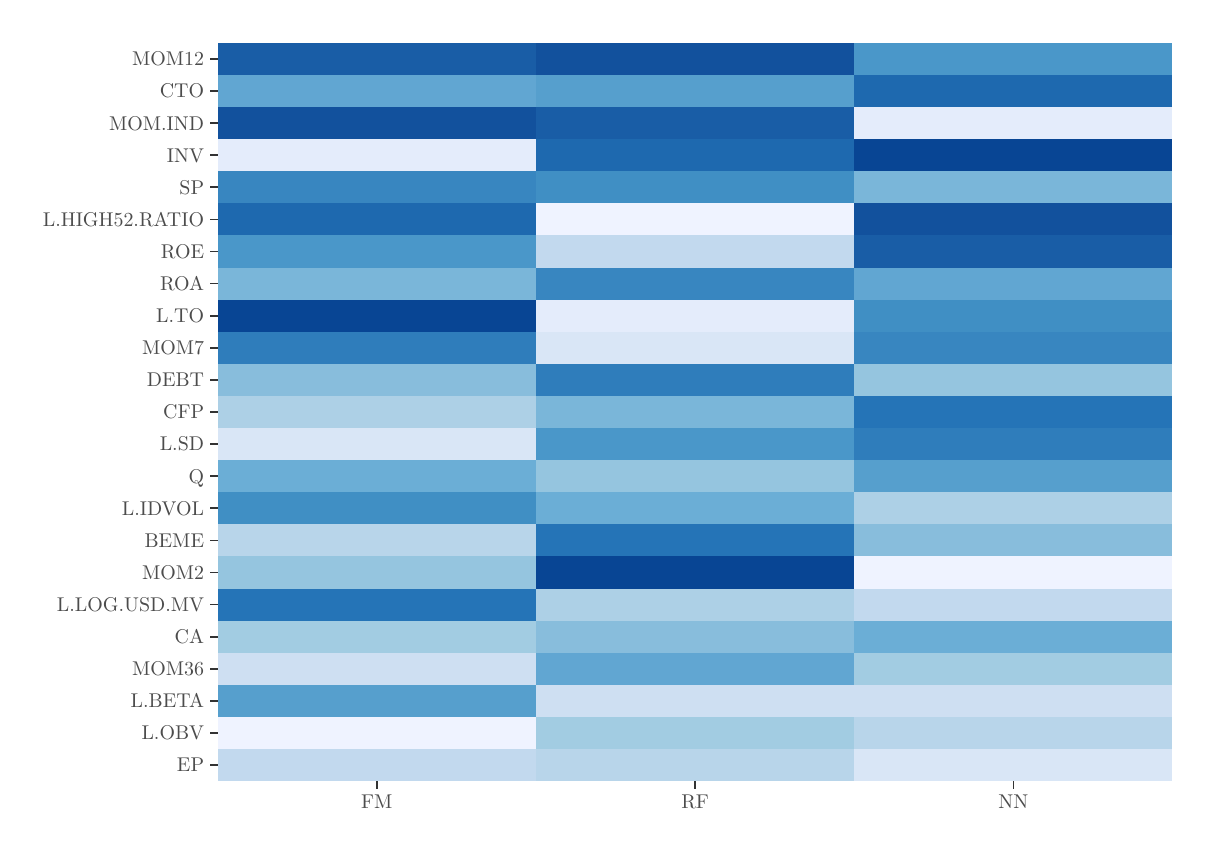
\begin{tikzpicture}[x=1pt,y=1pt]
\definecolor{fillColor}{RGB}{255,255,255}
\path[use as bounding box,fill=fillColor,fill opacity=0.00] (0,0) rectangle (419.17,289.08);
\begin{scope}
\path[clip] (  0.00,  0.00) rectangle (419.17,289.08);
\definecolor{drawColor}{RGB}{255,255,255}
\definecolor{fillColor}{RGB}{255,255,255}

\path[draw=drawColor,line width= 0.6pt,line join=round,line cap=round,fill=fillColor] (  0.00,  0.00) rectangle (419.17,289.08);
\end{scope}
\begin{scope}
\path[clip] ( 68.69, 16.81) rectangle (413.67,283.58);
\definecolor{fillColor}{gray}{0.92}

\path[fill=fillColor] ( 68.69, 16.81) rectangle (413.67,283.58);
\definecolor{drawColor}{RGB}{255,255,255}

\path[draw=drawColor,line width= 0.6pt,line join=round] ( 68.69, 22.61) --
	(413.67, 22.61);

\path[draw=drawColor,line width= 0.6pt,line join=round] ( 68.69, 34.21) --
	(413.67, 34.21);

\path[draw=drawColor,line width= 0.6pt,line join=round] ( 68.69, 45.81) --
	(413.67, 45.81);

\path[draw=drawColor,line width= 0.6pt,line join=round] ( 68.69, 57.40) --
	(413.67, 57.40);

\path[draw=drawColor,line width= 0.6pt,line join=round] ( 68.69, 69.00) --
	(413.67, 69.00);

\path[draw=drawColor,line width= 0.6pt,line join=round] ( 68.69, 80.60) --
	(413.67, 80.60);

\path[draw=drawColor,line width= 0.6pt,line join=round] ( 68.69, 92.20) --
	(413.67, 92.20);

\path[draw=drawColor,line width= 0.6pt,line join=round] ( 68.69,103.80) --
	(413.67,103.80);

\path[draw=drawColor,line width= 0.6pt,line join=round] ( 68.69,115.40) --
	(413.67,115.40);

\path[draw=drawColor,line width= 0.6pt,line join=round] ( 68.69,127.00) --
	(413.67,127.00);

\path[draw=drawColor,line width= 0.6pt,line join=round] ( 68.69,138.60) --
	(413.67,138.60);

\path[draw=drawColor,line width= 0.6pt,line join=round] ( 68.69,150.19) --
	(413.67,150.19);

\path[draw=drawColor,line width= 0.6pt,line join=round] ( 68.69,161.79) --
	(413.67,161.79);

\path[draw=drawColor,line width= 0.6pt,line join=round] ( 68.69,173.39) --
	(413.67,173.39);

\path[draw=drawColor,line width= 0.6pt,line join=round] ( 68.69,184.99) --
	(413.67,184.99);

\path[draw=drawColor,line width= 0.6pt,line join=round] ( 68.69,196.59) --
	(413.67,196.59);

\path[draw=drawColor,line width= 0.6pt,line join=round] ( 68.69,208.19) --
	(413.67,208.19);

\path[draw=drawColor,line width= 0.6pt,line join=round] ( 68.69,219.79) --
	(413.67,219.79);

\path[draw=drawColor,line width= 0.6pt,line join=round] ( 68.69,231.39) --
	(413.67,231.39);

\path[draw=drawColor,line width= 0.6pt,line join=round] ( 68.69,242.98) --
	(413.67,242.98);

\path[draw=drawColor,line width= 0.6pt,line join=round] ( 68.69,254.58) --
	(413.67,254.58);

\path[draw=drawColor,line width= 0.6pt,line join=round] ( 68.69,266.18) --
	(413.67,266.18);

\path[draw=drawColor,line width= 0.6pt,line join=round] ( 68.69,277.78) --
	(413.67,277.78);

\path[draw=drawColor,line width= 0.6pt,line join=round] (126.18, 16.81) --
	(126.18,283.58);

\path[draw=drawColor,line width= 0.6pt,line join=round] (241.18, 16.81) --
	(241.18,283.58);

\path[draw=drawColor,line width= 0.6pt,line join=round] (356.17, 16.81) --
	(356.17,283.58);
\definecolor{fillColor}{RGB}{37,116,183}

\path[fill=fillColor] (183.68, 98.00) rectangle (298.67,109.60);
\definecolor{fillColor}{RGB}{136,189,220}

\path[fill=fillColor] (183.68, 63.20) rectangle (298.67, 74.80);
\definecolor{fillColor}{RGB}{122,182,217}

\path[fill=fillColor] (183.68,144.39) rectangle (298.67,155.99);
\definecolor{fillColor}{RGB}{86,159,205}

\path[fill=fillColor] (183.68,260.38) rectangle (298.67,271.98);
\definecolor{fillColor}{RGB}{47,125,187}

\path[fill=fillColor] (183.68,155.99) rectangle (298.67,167.59);
\definecolor{fillColor}{RGB}{184,213,234}

\path[fill=fillColor] (183.68, 16.81) rectangle (298.67, 28.41);
\definecolor{fillColor}{RGB}{30,105,175}

\path[fill=fillColor] (183.68,237.18) rectangle (298.67,248.78);
\definecolor{fillColor}{RGB}{206,223,242}

\path[fill=fillColor] (183.68, 40.01) rectangle (298.67, 51.60);
\definecolor{fillColor}{RGB}{239,243,255}

\path[fill=fillColor] (183.68,213.99) rectangle (298.67,225.59);
\definecolor{fillColor}{RGB}{107,174,214}

\path[fill=fillColor] (183.68,109.60) rectangle (298.67,121.20);
\definecolor{fillColor}{RGB}{173,208,230}

\path[fill=fillColor] (183.68, 74.80) rectangle (298.67, 86.40);
\definecolor{fillColor}{RGB}{162,204,226}

\path[fill=fillColor] (183.68, 28.41) rectangle (298.67, 40.01);
\definecolor{fillColor}{RGB}{74,151,201}

\path[fill=fillColor] (183.68,132.80) rectangle (298.67,144.39);
\definecolor{fillColor}{RGB}{228,236,251}

\path[fill=fillColor] (183.68,179.19) rectangle (298.67,190.79);
\definecolor{fillColor}{RGB}{25,93,166}

\path[fill=fillColor] (183.68,248.78) rectangle (298.67,260.38);
\definecolor{fillColor}{RGB}{18,81,157}

\path[fill=fillColor] (183.68,271.98) rectangle (298.67,283.58);
\definecolor{fillColor}{RGB}{8,69,148}

\path[fill=fillColor] (183.68, 86.40) rectangle (298.67, 98.00);
\definecolor{fillColor}{RGB}{97,166,210}

\path[fill=fillColor] (183.68, 51.60) rectangle (298.67, 63.20);
\definecolor{fillColor}{RGB}{217,230,246}

\path[fill=fillColor] (183.68,167.59) rectangle (298.67,179.19);
\definecolor{fillColor}{RGB}{149,197,223}

\path[fill=fillColor] (183.68,121.20) rectangle (298.67,132.80);
\definecolor{fillColor}{RGB}{56,134,192}

\path[fill=fillColor] (183.68,190.79) rectangle (298.67,202.39);
\definecolor{fillColor}{RGB}{194,217,238}

\path[fill=fillColor] (183.68,202.39) rectangle (298.67,213.99);
\definecolor{fillColor}{RGB}{64,143,196}

\path[fill=fillColor] (183.68,225.59) rectangle (298.67,237.18);
\definecolor{fillColor}{RGB}{184,213,234}

\path[fill=fillColor] ( 68.69, 98.00) rectangle (183.68,109.60);
\definecolor{fillColor}{RGB}{162,204,226}

\path[fill=fillColor] ( 68.69, 63.20) rectangle (183.68, 74.80);
\definecolor{fillColor}{RGB}{173,208,230}

\path[fill=fillColor] ( 68.69,144.39) rectangle (183.68,155.99);
\definecolor{fillColor}{RGB}{97,166,210}

\path[fill=fillColor] ( 68.69,260.38) rectangle (183.68,271.98);
\definecolor{fillColor}{RGB}{136,189,220}

\path[fill=fillColor] ( 68.69,155.99) rectangle (183.68,167.59);
\definecolor{fillColor}{RGB}{194,217,238}

\path[fill=fillColor] ( 68.69, 16.81) rectangle (183.68, 28.41);
\definecolor{fillColor}{RGB}{228,236,251}

\path[fill=fillColor] ( 68.69,237.18) rectangle (183.68,248.78);
\definecolor{fillColor}{RGB}{86,159,205}

\path[fill=fillColor] ( 68.69, 40.01) rectangle (183.68, 51.60);
\definecolor{fillColor}{RGB}{30,105,175}

\path[fill=fillColor] ( 68.69,213.99) rectangle (183.68,225.59);
\definecolor{fillColor}{RGB}{64,143,196}

\path[fill=fillColor] ( 68.69,109.60) rectangle (183.68,121.20);
\definecolor{fillColor}{RGB}{37,116,183}

\path[fill=fillColor] ( 68.69, 74.80) rectangle (183.68, 86.40);
\definecolor{fillColor}{RGB}{239,243,255}

\path[fill=fillColor] ( 68.69, 28.41) rectangle (183.68, 40.01);
\definecolor{fillColor}{RGB}{217,230,246}

\path[fill=fillColor] ( 68.69,132.80) rectangle (183.68,144.39);
\definecolor{fillColor}{RGB}{8,69,148}

\path[fill=fillColor] ( 68.69,179.19) rectangle (183.68,190.79);
\definecolor{fillColor}{RGB}{18,81,157}

\path[fill=fillColor] ( 68.69,248.78) rectangle (183.68,260.38);
\definecolor{fillColor}{RGB}{25,93,166}

\path[fill=fillColor] ( 68.69,271.98) rectangle (183.68,283.58);
\definecolor{fillColor}{RGB}{149,197,223}

\path[fill=fillColor] ( 68.69, 86.40) rectangle (183.68, 98.00);
\definecolor{fillColor}{RGB}{206,223,242}

\path[fill=fillColor] ( 68.69, 51.60) rectangle (183.68, 63.20);
\definecolor{fillColor}{RGB}{47,125,187}

\path[fill=fillColor] ( 68.69,167.59) rectangle (183.68,179.19);
\definecolor{fillColor}{RGB}{107,174,214}

\path[fill=fillColor] ( 68.69,121.20) rectangle (183.68,132.80);
\definecolor{fillColor}{RGB}{122,182,217}

\path[fill=fillColor] ( 68.69,190.79) rectangle (183.68,202.39);
\definecolor{fillColor}{RGB}{74,151,201}

\path[fill=fillColor] ( 68.69,202.39) rectangle (183.68,213.99);
\definecolor{fillColor}{RGB}{56,134,192}

\path[fill=fillColor] ( 68.69,225.59) rectangle (183.68,237.18);
\definecolor{fillColor}{RGB}{136,189,220}

\path[fill=fillColor] (298.67, 98.00) rectangle (413.67,109.60);
\definecolor{fillColor}{RGB}{107,174,214}

\path[fill=fillColor] (298.67, 63.20) rectangle (413.67, 74.80);
\definecolor{fillColor}{RGB}{37,116,183}

\path[fill=fillColor] (298.67,144.39) rectangle (413.67,155.99);
\definecolor{fillColor}{RGB}{30,105,175}

\path[fill=fillColor] (298.67,260.38) rectangle (413.67,271.98);
\definecolor{fillColor}{RGB}{149,197,223}

\path[fill=fillColor] (298.67,155.99) rectangle (413.67,167.59);
\definecolor{fillColor}{RGB}{217,230,246}

\path[fill=fillColor] (298.67, 16.81) rectangle (413.67, 28.41);
\definecolor{fillColor}{RGB}{8,69,148}

\path[fill=fillColor] (298.67,237.18) rectangle (413.67,248.78);
\definecolor{fillColor}{RGB}{206,223,242}

\path[fill=fillColor] (298.67, 40.01) rectangle (413.67, 51.60);
\definecolor{fillColor}{RGB}{18,81,157}

\path[fill=fillColor] (298.67,213.99) rectangle (413.67,225.59);
\definecolor{fillColor}{RGB}{173,208,230}

\path[fill=fillColor] (298.67,109.60) rectangle (413.67,121.20);
\definecolor{fillColor}{RGB}{194,217,238}

\path[fill=fillColor] (298.67, 74.80) rectangle (413.67, 86.40);
\definecolor{fillColor}{RGB}{184,213,234}

\path[fill=fillColor] (298.67, 28.41) rectangle (413.67, 40.01);
\definecolor{fillColor}{RGB}{47,125,187}

\path[fill=fillColor] (298.67,132.80) rectangle (413.67,144.39);
\definecolor{fillColor}{RGB}{64,143,196}

\path[fill=fillColor] (298.67,179.19) rectangle (413.67,190.79);
\definecolor{fillColor}{RGB}{228,236,251}

\path[fill=fillColor] (298.67,248.78) rectangle (413.67,260.38);
\definecolor{fillColor}{RGB}{74,151,201}

\path[fill=fillColor] (298.67,271.98) rectangle (413.67,283.58);
\definecolor{fillColor}{RGB}{239,243,255}

\path[fill=fillColor] (298.67, 86.40) rectangle (413.67, 98.00);
\definecolor{fillColor}{RGB}{162,204,226}

\path[fill=fillColor] (298.67, 51.60) rectangle (413.67, 63.20);
\definecolor{fillColor}{RGB}{56,134,192}

\path[fill=fillColor] (298.67,167.59) rectangle (413.67,179.19);
\definecolor{fillColor}{RGB}{86,159,205}

\path[fill=fillColor] (298.67,121.20) rectangle (413.67,132.80);
\definecolor{fillColor}{RGB}{97,166,210}

\path[fill=fillColor] (298.67,190.79) rectangle (413.67,202.39);
\definecolor{fillColor}{RGB}{25,93,166}

\path[fill=fillColor] (298.67,202.39) rectangle (413.67,213.99);
\definecolor{fillColor}{RGB}{122,182,217}

\path[fill=fillColor] (298.67,225.59) rectangle (413.67,237.18);
\end{scope}
\begin{scope}
\path[clip] (  0.00,  0.00) rectangle (419.17,289.08);
\definecolor{drawColor}{gray}{0.30}

\node[text=drawColor,anchor=base east,inner sep=0pt, outer sep=0pt, scale=  0.72] at ( 63.74, 20.13) {EP};

\node[text=drawColor,anchor=base east,inner sep=0pt, outer sep=0pt, scale=  0.72] at ( 63.74, 31.73) {L.OBV};

\node[text=drawColor,anchor=base east,inner sep=0pt, outer sep=0pt, scale=  0.72] at ( 63.74, 43.33) {L.BETA};

\node[text=drawColor,anchor=base east,inner sep=0pt, outer sep=0pt, scale=  0.72] at ( 63.74, 54.92) {MOM36};

\node[text=drawColor,anchor=base east,inner sep=0pt, outer sep=0pt, scale=  0.72] at ( 63.74, 66.52) {CA};

\node[text=drawColor,anchor=base east,inner sep=0pt, outer sep=0pt, scale=  0.72] at ( 63.74, 78.12) {L.LOG.USD.MV};

\node[text=drawColor,anchor=base east,inner sep=0pt, outer sep=0pt, scale=  0.72] at ( 63.74, 89.72) {MOM2};

\node[text=drawColor,anchor=base east,inner sep=0pt, outer sep=0pt, scale=  0.72] at ( 63.74,101.32) {BEME};

\node[text=drawColor,anchor=base east,inner sep=0pt, outer sep=0pt, scale=  0.72] at ( 63.74,112.92) {L.IDVOL};

\node[text=drawColor,anchor=base east,inner sep=0pt, outer sep=0pt, scale=  0.72] at ( 63.74,124.52) {Q};

\node[text=drawColor,anchor=base east,inner sep=0pt, outer sep=0pt, scale=  0.72] at ( 63.74,136.12) {L.SD};

\node[text=drawColor,anchor=base east,inner sep=0pt, outer sep=0pt, scale=  0.72] at ( 63.74,147.71) {CFP};

\node[text=drawColor,anchor=base east,inner sep=0pt, outer sep=0pt, scale=  0.72] at ( 63.74,159.31) {DEBT};

\node[text=drawColor,anchor=base east,inner sep=0pt, outer sep=0pt, scale=  0.72] at ( 63.74,170.91) {MOM7};

\node[text=drawColor,anchor=base east,inner sep=0pt, outer sep=0pt, scale=  0.72] at ( 63.74,182.51) {L.TO};

\node[text=drawColor,anchor=base east,inner sep=0pt, outer sep=0pt, scale=  0.72] at ( 63.74,194.11) {ROA};

\node[text=drawColor,anchor=base east,inner sep=0pt, outer sep=0pt, scale=  0.72] at ( 63.74,205.71) {ROE};

\node[text=drawColor,anchor=base east,inner sep=0pt, outer sep=0pt, scale=  0.72] at ( 63.74,217.31) {L.HIGH52.RATIO};

\node[text=drawColor,anchor=base east,inner sep=0pt, outer sep=0pt, scale=  0.72] at ( 63.74,228.91) {SP};

\node[text=drawColor,anchor=base east,inner sep=0pt, outer sep=0pt, scale=  0.72] at ( 63.74,240.50) {INV};

\node[text=drawColor,anchor=base east,inner sep=0pt, outer sep=0pt, scale=  0.72] at ( 63.74,252.10) {MOM.IND};

\node[text=drawColor,anchor=base east,inner sep=0pt, outer sep=0pt, scale=  0.72] at ( 63.74,263.70) {CTO};

\node[text=drawColor,anchor=base east,inner sep=0pt, outer sep=0pt, scale=  0.72] at ( 63.74,275.30) {MOM12};
\end{scope}
\begin{scope}
\path[clip] (  0.00,  0.00) rectangle (419.17,289.08);
\definecolor{drawColor}{gray}{0.20}

\path[draw=drawColor,line width= 0.6pt,line join=round] ( 65.94, 22.61) --
	( 68.69, 22.61);

\path[draw=drawColor,line width= 0.6pt,line join=round] ( 65.94, 34.21) --
	( 68.69, 34.21);

\path[draw=drawColor,line width= 0.6pt,line join=round] ( 65.94, 45.81) --
	( 68.69, 45.81);

\path[draw=drawColor,line width= 0.6pt,line join=round] ( 65.94, 57.40) --
	( 68.69, 57.40);

\path[draw=drawColor,line width= 0.6pt,line join=round] ( 65.94, 69.00) --
	( 68.69, 69.00);

\path[draw=drawColor,line width= 0.6pt,line join=round] ( 65.94, 80.60) --
	( 68.69, 80.60);

\path[draw=drawColor,line width= 0.6pt,line join=round] ( 65.94, 92.20) --
	( 68.69, 92.20);

\path[draw=drawColor,line width= 0.6pt,line join=round] ( 65.94,103.80) --
	( 68.69,103.80);

\path[draw=drawColor,line width= 0.6pt,line join=round] ( 65.94,115.40) --
	( 68.69,115.40);

\path[draw=drawColor,line width= 0.6pt,line join=round] ( 65.94,127.00) --
	( 68.69,127.00);

\path[draw=drawColor,line width= 0.6pt,line join=round] ( 65.94,138.60) --
	( 68.69,138.60);

\path[draw=drawColor,line width= 0.6pt,line join=round] ( 65.94,150.19) --
	( 68.69,150.19);

\path[draw=drawColor,line width= 0.6pt,line join=round] ( 65.94,161.79) --
	( 68.69,161.79);

\path[draw=drawColor,line width= 0.6pt,line join=round] ( 65.94,173.39) --
	( 68.69,173.39);

\path[draw=drawColor,line width= 0.6pt,line join=round] ( 65.94,184.99) --
	( 68.69,184.99);

\path[draw=drawColor,line width= 0.6pt,line join=round] ( 65.94,196.59) --
	( 68.69,196.59);

\path[draw=drawColor,line width= 0.6pt,line join=round] ( 65.94,208.19) --
	( 68.69,208.19);

\path[draw=drawColor,line width= 0.6pt,line join=round] ( 65.94,219.79) --
	( 68.69,219.79);

\path[draw=drawColor,line width= 0.6pt,line join=round] ( 65.94,231.39) --
	( 68.69,231.39);

\path[draw=drawColor,line width= 0.6pt,line join=round] ( 65.94,242.98) --
	( 68.69,242.98);

\path[draw=drawColor,line width= 0.6pt,line join=round] ( 65.94,254.58) --
	( 68.69,254.58);

\path[draw=drawColor,line width= 0.6pt,line join=round] ( 65.94,266.18) --
	( 68.69,266.18);

\path[draw=drawColor,line width= 0.6pt,line join=round] ( 65.94,277.78) --
	( 68.69,277.78);
\end{scope}
\begin{scope}
\path[clip] (  0.00,  0.00) rectangle (419.17,289.08);
\definecolor{drawColor}{gray}{0.20}

\path[draw=drawColor,line width= 0.6pt,line join=round] (126.18, 14.06) --
	(126.18, 16.81);

\path[draw=drawColor,line width= 0.6pt,line join=round] (241.18, 14.06) --
	(241.18, 16.81);

\path[draw=drawColor,line width= 0.6pt,line join=round] (356.17, 14.06) --
	(356.17, 16.81);
\end{scope}
\begin{scope}
\path[clip] (  0.00,  0.00) rectangle (419.17,289.08);
\definecolor{drawColor}{gray}{0.30}

\node[text=drawColor,anchor=base,inner sep=0pt, outer sep=0pt, scale=  0.72] at (126.18,  6.90) {FM};

\node[text=drawColor,anchor=base,inner sep=0pt, outer sep=0pt, scale=  0.72] at (241.18,  6.90) {RF};

\node[text=drawColor,anchor=base,inner sep=0pt, outer sep=0pt, scale=  0.72] at (356.17,  6.90) {NN};
\end{scope}
\end{tikzpicture}

\label{plot:combined_VI}
\end{figure}

\appendix
\section{Data}
\renewcommand{\thefigure}{A.\arabic{figure}}
\setcounter{figure}{0}
\renewcommand{\thetable}{A.\arabic{table}}
\setcounter{table}{0}

\begin{table}[h] 
\small
\caption[Constituent lists and keywords]{\textbf{Constituent lists and keywords}\\ Table provides the constituent lists used in data collection.}
 \label{table:constituteLists}
\centering
\begin{tabularx}{\textwidth}{X X X X}
\toprule
Denmark & Finland & Norway & Sweden \\
\midrule
FDEN 		&  FFIN		& FNOR		& FSWD\\
WSCOPEDK & WSCOPEFN & WSCOPENW& WSCOPESD\\
DEADDK 	&   DEADFN 	& DEADNW 	& DEADSD\\
& & & FAKTSWD\\
 \bottomrule
 \end{tabularx}
 \end{table} 

\begin{table}[h]
\small
\caption[Static screens]{\textbf{Static screens}\\ It also provides the country specific keywords that are used to deleted entries from the dataset. Panel B provides keywords that were used to delete entries from each market separately. Keyword deletion follows Ince and Porter \protect\citeyear{Ince2006} and Hanauer and Windmüller \protect\citeyear{HANAUER2023106712}. Same logic is applied to remove both country specific and generic keywords. Keyword is searched from Datastream attributes NAME, ENAME and ECNAME. In case if at least one of these attributes contains the keyword security is deleted from the dataset. To avoid deleting proper entries, security is only deleted if keyword occurs at the beginning of the name, at the end of the name or as separate word in the name.}
\label{table:staticscreens}
\begin{tabularx}{\textwidth}{X X X X l}
\toprule
\multicolumn{5}{l}{\textit{Panel A: Static screens.}} \\
\midrule
 & Denmark & Finland & Norway & Sweden\\
\midrule
MAJOR & Y & Y & Y & Y\\
TYPE & EQ & EQ & EQ & EQ\\
ISINID & P & P & P & P\\
GEOGN & DENMARK & FINLAND & NORWAY & SWEDEN\\
GEOLN & DENMARK & FINLAND & NORWAY & SWEDEN\\
PCUR & DK & FI, MK & NK & SK\\
GGSIN & DK & FI & NO &SE\\
\toprule
\multicolumn{5}{l}{\textit{Panel B: Country specific keywords.}} \\
\midrule
 & Denmark & Finland & Norway & Sweden\\
 \midrule
NAME & \multirow[m]{3}{*}{ \textbackslash \textbackslash)CSE \textbackslash \textbackslash} & \multirow[m]{3}{*}{USE} & & \multirow[m]{3}{13em}{CONVERTED INTO, USE, CONVERTED-, CONVERTED - SEE}\\
ENAME & & \\
ECNAME & &\\
\bottomrule
\end{tabularx}
\end{table}


\begin{table}[h] 
\small
\caption[Country specific keywords]{\textbf{Country specific keywords}\\ Table shows the general keywords that were used to delete entries from all markets. Keyword deletion follows Ince and Porter \protect\citeyear{Ince2006} and Hanauer and Windmüller \protect\citeyear{HANAUER2023106712}. Same logic is applied to remove both country specific and generic keywords. Keyword is searched from Datastream attributes NAME, ENAME and ECNAME. In case if at least one of these attributes contains the keyword security is deleted from the dataset. To avoid deleting proper entries, security is only deleted if keyword occurs at the beginning of the name, at the end of the name or as separate word in the name.}
 \label{table:generalKeywords}
\centering
\begin{tabularx}{\textwidth}{l X}
\toprule
Security class 	& Keywords \\
\midrule
Duplicates 		& 1000DUPL, DULP, DUP, DUPE, DUPL, DUPLI, DUPLICATE, XSQ, XETa  \\[1ex]
Depository receipts	& ADR, GDR \\[1ex]
Preferred stock 	&  PF, ’PF’, PFD, PREF, PREFERRED, PRF\\ [1ex]
Warrants 			&  WARR, WARRANT, WARRANTS, WARRT, WTS, WTS2\\[1ex]
Debt 			& \%, DB, DCB, DEB, DEBENTURE, DEBENTURES, DEBT\\[1ex]
Unit trusts 		& .IT, .ITb, TST, INVESTMENTTRUST, RLSTIT, TRUST, TRUSTUNIT, TRUSTUNITS, TST, TSTUNIT, TST UNITS, UNIT, UNITTRUST, UNITS, UNT, UNTTST, UT\\[1ex]
ETFs 			& AMUNDI, ETF, INAV, ISHARES, JUNGE, LYXOR, X-TR\\[1ex]
Expired securities 	& EXPD, EXPIRED, EXPIRY, EXPY\\[1ex]
Miscellaneous 		& ADS, BOND, CAP.SHS, CONV, DEFER, DEP, DEPY, ELKS, FD, FUND, GW.FD, HI.YIELD, HIGHINCOME, IDX, INC.								\&GROWTH, INC.\&GW, INDEX, LP, MITS, MITT, MPS, NIKKEI, OPCVM, ORTF, PERQS, 												PFC, PFCL, PINES, PRTF, PTNS, PTSHP, QUIBS, QUIDS, RATE, RCPTS, REALEST, RECEIPTS, REIT, RESPT, 								RETUR, RIGHTS, RST, RTN.INC, RTS, SBVTG, SCORE, SPDR, STRYPES, TOPRS, UTS, VCT, VTG.SAS, 									XXXXX, YIELD,YLD, PF.SHS.\\
 \bottomrule
 \end{tabularx}
 \end{table} 


\begin{table}[h] 
\small
\caption[Variable definitions]{\textbf{Variable definitions} \\Tables provides definitions and initial authors for all anomalies used in the study. Construction of variables follows Green et. al \protect\citeyear{Green2017} and Hanauer and Kalsbach \protect\citeyear{HANAUER2022}.}
\label{table:variableDefs}
\centering
\begin{tabularx}{\textwidth}{l X X}
\toprule
Variable & Author & Definition\\
\midrule
Cash-to-Assets 		& \cite{PALAZZO2012162} 	& Cash-to-Asset ratio is calculated by dividing  cash and short-term investments by total assets.\\
Capital Turnover 		& i						& Capital turnover is calculated by dividing total sales by one year lagged total assets.\\
Investment 			& i						& Investments are defined as a yearly change in total assets.\\	
Book-to-Market Equity 	& \cite{Rosenberg1985} 		&  Book-to-Market value is calculated by dividing company's book value of equity by company's market 										 	capitaliztion end of previous year. Book value of equity is calculated by summing common 												equity and deferred taxes of the company. \\
Cash Flow-to-Price 		& \cite{LAKONISHOK1994} 	& Cash flow to price ratio is calculated by dividing company's cash flow from operating activities 												by the asset's market capitaliztion end of previous year. \\
Debt-to-Price			& i						& Debt-to-price value is calculated as difference between total assets and common equity 													divided by the asset's market capitaliztion end of previous year.\\
Sales-to-Price 			& i						& Sales-to-price ratio is calculated by dividing total sales by asset's market capitaliztion end of 													previous year.\\
Earnings-to-Price 		& i						& Earnings-to-price ratio is calculated by dividing net income before extra Items and preferred 													dividends by asset's market capitaliztion end of previous year.\\
Return-on-Assets 		& i						& Return-on-assets is calculated as net income before extra Items and preferred dividends divided 												by one year lagged total assets.\\
Return-on-Equity 		& i						& Return-on-equity is calculated as net income before extra Items and preferred dividends divided 												by one year lagged book value of equity. See book-to-market equity for definition of book 													value of equity. \\
Tobin's Q 				& i						& tbd\\
Momentum$_{7}$ 		& i						& Cumulative return in US dollars between $t-7$ and $t-12$ months.\\
Momentum$_{12}$ 		& i						& Cumulative return in US dollars between $t-2$ and $t-12$ months.\\
Momentum$_{36}$ 		& i						& Cumulative return in US dollars between $t-12$ and $t-36$ months.\\
Momentum$_{2}$ 		& i						& Prior month return in US dollars.\\ 
\bottomrule
\end{tabularx}
\end{table} 

\begin{figure}[h]
\centering
\caption[Number of companies]{\textbf{Number of companies}\\ Figure shows the development of total number of securities considered in the dataset from 1990 to 2022 for each Nordic country. Figures counts all securities that passed the static screens. Final amount of companies in each time point can be lower since security will be excluded from the dataset if it is missing certain information.}
% Created by tikzDevice version 0.12.6 on 2024-03-22 10:26:56
% !TEX encoding = UTF-8 Unicode
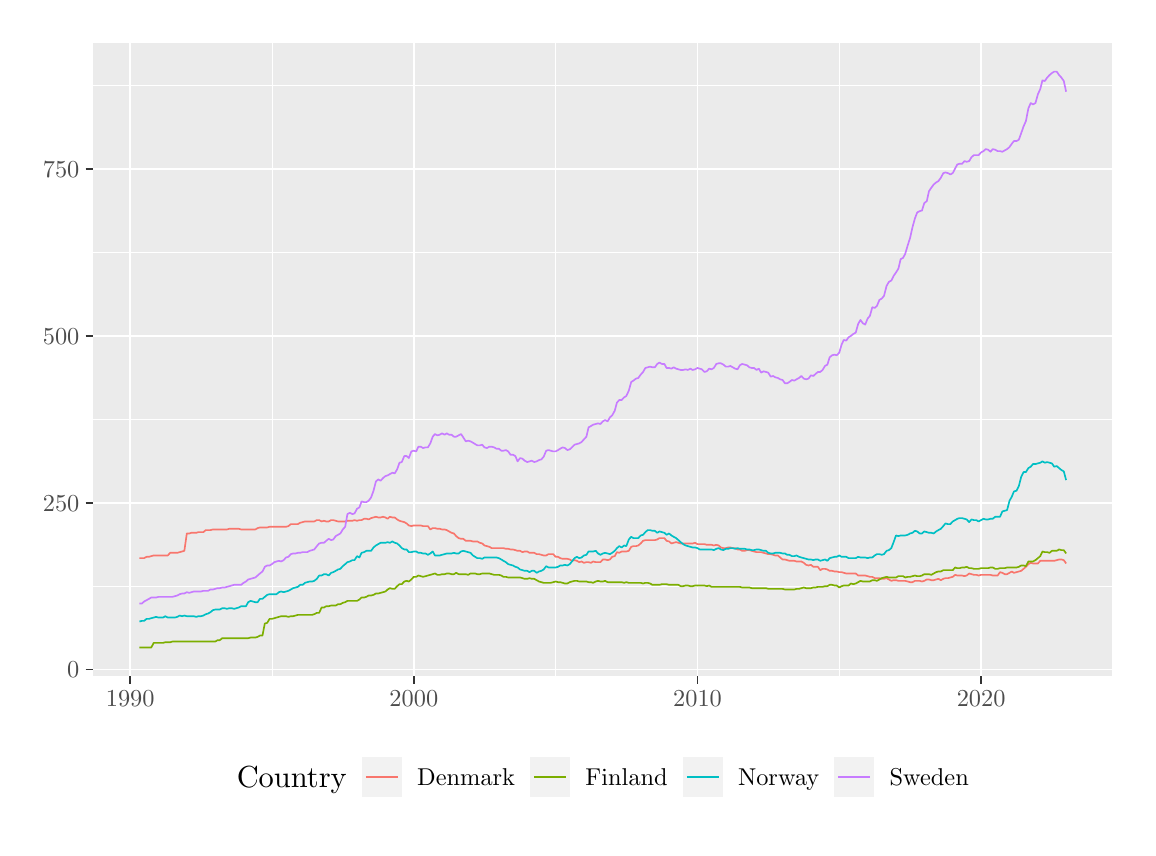
\begin{tikzpicture}[x=1pt,y=1pt]
\definecolor{fillColor}{RGB}{255,255,255}
\path[use as bounding box,fill=fillColor,fill opacity=0.00] (0,0) rectangle (397.48,289.08);
\begin{scope}
\path[clip] (  0.00,  0.00) rectangle (397.48,289.08);
\definecolor{drawColor}{RGB}{255,255,255}
\definecolor{fillColor}{RGB}{255,255,255}

\path[draw=drawColor,line width= 0.6pt,line join=round,line cap=round,fill=fillColor] (  0.00,  0.00) rectangle (397.48,289.08);
\end{scope}
\begin{scope}
\path[clip] ( 23.65, 54.68) rectangle (391.98,283.58);
\definecolor{fillColor}{gray}{0.92}

\path[fill=fillColor] ( 23.65, 54.68) rectangle (391.98,283.58);
\definecolor{drawColor}{RGB}{255,255,255}

\path[draw=drawColor,line width= 0.3pt,line join=round] ( 23.65, 87.26) --
	(391.98, 87.26);

\path[draw=drawColor,line width= 0.3pt,line join=round] ( 23.65,147.55) --
	(391.98,147.55);

\path[draw=drawColor,line width= 0.3pt,line join=round] ( 23.65,207.83) --
	(391.98,207.83);

\path[draw=drawColor,line width= 0.3pt,line join=round] ( 23.65,268.11) --
	(391.98,268.11);

\path[draw=drawColor,line width= 0.3pt,line join=round] ( 88.29, 54.68) --
	( 88.29,283.58);

\path[draw=drawColor,line width= 0.3pt,line join=round] (190.80, 54.68) --
	(190.80,283.58);

\path[draw=drawColor,line width= 0.3pt,line join=round] (293.30, 54.68) --
	(293.30,283.58);

\path[draw=drawColor,line width= 0.6pt,line join=round] ( 23.65, 57.12) --
	(391.98, 57.12);

\path[draw=drawColor,line width= 0.6pt,line join=round] ( 23.65,117.41) --
	(391.98,117.41);

\path[draw=drawColor,line width= 0.6pt,line join=round] ( 23.65,177.69) --
	(391.98,177.69);

\path[draw=drawColor,line width= 0.6pt,line join=round] ( 23.65,237.97) --
	(391.98,237.97);

\path[draw=drawColor,line width= 0.6pt,line join=round] ( 37.05, 54.68) --
	( 37.05,283.58);

\path[draw=drawColor,line width= 0.6pt,line join=round] (139.54, 54.68) --
	(139.54,283.58);

\path[draw=drawColor,line width= 0.6pt,line join=round] (242.05, 54.68) --
	(242.05,283.58);

\path[draw=drawColor,line width= 0.6pt,line join=round] (344.54, 54.68) --
	(344.54,283.58);
\definecolor{drawColor}{RGB}{248,118,109}

\path[draw=drawColor,line width= 0.6pt,line join=round] ( 40.39, 97.39) --
	( 41.26, 97.39) --
	( 42.07, 97.39) --
	( 42.97, 97.87) --
	( 43.84, 97.87) --
	( 44.63, 98.12) --
	( 45.55, 98.36) --
	( 46.40, 98.36) --
	( 47.27, 98.36) --
	( 48.13, 98.36) --
	( 48.92, 98.36) --
	( 49.73, 98.36) --
	( 50.63, 98.36) --
	( 51.50, 99.32) --
	( 52.29, 99.32) --
	( 53.21, 99.32) --
	( 54.06, 99.32) --
	( 54.93, 99.56) --
	( 55.80, 99.80) --
	( 56.61,100.04) --
	( 57.51,106.31) --
	( 58.38,106.31) --
	( 59.16,106.55) --
	( 60.06,106.55) --
	( 60.90,106.55) --
	( 61.72,106.80) --
	( 62.62,106.80) --
	( 63.49,106.80) --
	( 64.36,107.52) --
	( 65.20,107.52) --
	( 66.04,107.52) --
	( 66.91,107.76) --
	( 67.78,107.76) --
	( 68.59,107.76) --
	( 69.38,107.76) --
	( 70.31,107.76) --
	( 71.15,107.76) --
	( 72.02,107.76) --
	( 72.86,108.00) --
	( 73.70,108.00) --
	( 74.60,108.00) --
	( 75.44,108.00) --
	( 76.25,108.00) --
	( 77.15,107.76) --
	( 78.02,107.76) --
	( 78.89,107.76) --
	( 79.68,107.76) --
	( 80.55,107.76) --
	( 81.36,107.76) --
	( 82.26,107.76) --
	( 83.10,108.24) --
	( 83.92,108.48) --
	( 84.84,108.48) --
	( 85.68,108.48) --
	( 86.55,108.48) --
	( 87.40,108.72) --
	( 88.24,108.72) --
	( 89.14,108.72) --
	( 89.92,108.72) --
	( 90.79,108.72) --
	( 91.58,108.72) --
	( 92.50,108.72) --
	( 93.35,108.72) --
	( 94.22,108.97) --
	( 95.09,109.69) --
	( 95.90,109.69) --
	( 96.80,109.69) --
	( 97.64,109.69) --
	( 98.45,110.17) --
	( 99.38,110.41) --
	(100.19,110.65) --
	(101.01,110.65) --
	(101.90,110.65) --
	(102.77,110.65) --
	(103.56,110.65) --
	(104.49,111.14) --
	(105.33,111.14) --
	(106.20,110.65) --
	(107.07,110.89) --
	(107.88,110.65) --
	(108.78,110.65) --
	(109.65,111.14) --
	(110.44,111.14) --
	(111.31,110.89) --
	(112.15,110.65) --
	(112.99,110.65) --
	(113.86,110.65) --
	(114.73,110.65) --
	(115.54,110.89) --
	(116.44,110.89) --
	(117.31,110.89) --
	(118.10,111.14) --
	(119.02,110.89) --
	(119.87,111.14) --
	(120.65,111.14) --
	(121.55,111.62) --
	(122.39,111.62) --
	(123.20,111.38) --
	(124.10,111.86) --
	(124.97,112.10) --
	(125.84,112.34) --
	(126.68,112.10) --
	(127.53,112.10) --
	(128.40,112.34) --
	(129.27,112.10) --
	(130.08,111.62) --
	(130.87,112.34) --
	(131.79,112.10) --
	(132.63,112.10) --
	(133.50,111.38) --
	(134.35,110.89) --
	(135.19,110.65) --
	(136.09,110.41) --
	(136.93,109.93) --
	(137.74,109.21) --
	(138.64,108.97) --
	(139.51,109.21) --
	(140.38,109.21) --
	(141.19,109.21) --
	(142.06,109.21) --
	(142.85,108.97) --
	(143.78,108.97) --
	(144.62,108.97) --
	(145.49,107.76) --
	(146.36,108.24) --
	(147.17,108.24) --
	(148.07,108.00) --
	(148.91,108.00) --
	(149.72,107.76) --
	(150.65,107.76) --
	(151.44,107.52) --
	(152.28,107.04) --
	(153.15,106.55) --
	(154.02,106.31) --
	(154.83,105.35) --
	(155.73,104.63) --
	(156.60,104.38) --
	(157.39,104.38) --
	(158.31,103.66) --
	(159.15,103.66) --
	(160.02,103.66) --
	(160.89,103.42) --
	(161.68,103.42) --
	(162.49,103.42) --
	(163.39,102.94) --
	(164.26,102.70) --
	(165.05,101.97) --
	(165.97,101.73) --
	(166.82,101.49) --
	(167.69,101.01) --
	(168.56,101.01) --
	(169.37,101.01) --
	(170.27,101.01) --
	(171.14,101.01) --
	(171.92,101.01) --
	(172.79,100.77) --
	(173.63,100.77) --
	(174.48,100.53) --
	(175.35,100.53) --
	(176.22,100.29) --
	(177.03,100.04) --
	(177.93,100.04) --
	(178.80, 99.56) --
	(179.58, 99.80) --
	(180.51, 99.80) --
	(181.35, 99.32) --
	(182.14, 99.32) --
	(183.06, 99.32) --
	(183.91, 98.84) --
	(184.78, 98.84) --
	(185.62, 98.60) --
	(186.46, 98.36) --
	(187.36, 98.36) --
	(188.20, 98.84) --
	(189.01, 98.84) --
	(189.91, 98.84) --
	(190.78, 97.87) --
	(191.65, 97.87) --
	(192.44, 97.39) --
	(193.31, 97.15) --
	(194.12, 97.15) --
	(195.02, 97.15) --
	(195.86, 96.91) --
	(196.67, 96.43) --
	(197.60, 96.67) --
	(198.44, 96.43) --
	(199.31, 95.94) --
	(200.15, 96.19) --
	(201.00, 95.70) --
	(201.89, 95.94) --
	(202.68, 95.94) --
	(203.55, 95.70) --
	(204.34, 96.19) --
	(205.26, 95.94) --
	(206.10, 95.94) --
	(206.97, 95.94) --
	(207.84, 96.91) --
	(208.66, 96.91) --
	(209.56, 96.67) --
	(210.40, 96.91) --
	(211.21, 97.87) --
	(212.14, 98.12) --
	(212.92, 99.56) --
	(213.77, 99.32) --
	(214.64, 99.80) --
	(215.51, 99.80) --
	(216.32, 99.80) --
	(217.22,100.04) --
	(218.09,101.49) --
	(218.87,101.73) --
	(219.80,101.73) --
	(220.64,101.97) --
	(221.51,102.70) --
	(222.38,103.66) --
	(223.19,103.90) --
	(224.06,103.90) --
	(224.91,103.90) --
	(225.75,103.90) --
	(226.62,103.90) --
	(227.49,104.14) --
	(228.30,104.63) --
	(229.20,104.63) --
	(230.07,104.63) --
	(230.86,103.66) --
	(231.78,103.42) --
	(232.62,102.70) --
	(233.41,102.94) --
	(234.31,103.18) --
	(235.15,102.94) --
	(235.96,102.70) --
	(236.86,102.70) --
	(237.73,102.70) --
	(238.60,102.70) --
	(239.44,102.70) --
	(240.29,102.70) --
	(241.16,102.94) --
	(242.03,102.46) --
	(242.84,102.46) --
	(243.62,102.46) --
	(244.55,102.46) --
	(245.39,102.21) --
	(246.26,102.21) --
	(247.10,102.21) --
	(247.95,101.97) --
	(248.84,102.21) --
	(249.69,101.97) --
	(250.50,101.25) --
	(251.40,101.01) --
	(252.27,101.01) --
	(253.14,101.25) --
	(253.92,101.25) --
	(254.79,101.01) --
	(255.61,101.01) --
	(256.51,100.53) --
	(257.35,100.53) --
	(258.16,100.04) --
	(259.09,100.04) --
	(259.93,100.29) --
	(260.80,100.29) --
	(261.64,100.04) --
	(262.48, 99.80) --
	(263.38, 99.56) --
	(264.20, 99.56) --
	(265.04, 99.56) --
	(265.91, 99.32) --
	(266.78, 99.08) --
	(267.59, 98.84) --
	(268.49, 98.84) --
	(269.36, 98.60) --
	(270.14, 98.36) --
	(271.07, 98.36) --
	(271.91, 97.63) --
	(272.78, 96.91) --
	(273.65, 96.91) --
	(274.44, 96.67) --
	(275.25, 96.43) --
	(276.15, 96.43) --
	(277.02, 96.43) --
	(277.81, 96.19) --
	(278.73, 96.19) --
	(279.57, 96.19) --
	(280.44, 95.70) --
	(281.31, 94.98) --
	(282.13, 94.74) --
	(283.03, 94.98) --
	(283.90, 94.26) --
	(284.68, 94.26) --
	(285.55, 94.26) --
	(286.39, 93.05) --
	(287.24, 93.53) --
	(288.11, 93.53) --
	(288.98, 93.29) --
	(289.79, 92.81) --
	(290.69, 92.81) --
	(291.56, 92.57) --
	(292.34, 92.57) --
	(293.27, 92.33) --
	(294.11, 92.33) --
	(294.90, 92.09) --
	(295.79, 91.85) --
	(296.64, 91.85) --
	(297.45, 91.85) --
	(298.35, 91.85) --
	(299.22, 91.85) --
	(300.09, 91.12) --
	(300.93, 91.12) --
	(301.77, 91.12) --
	(302.64, 91.12) --
	(303.51, 90.88) --
	(304.33, 90.64) --
	(305.20, 90.64) --
	(306.07, 90.16) --
	(306.88, 90.16) --
	(307.78, 90.16) --
	(308.62, 89.92) --
	(309.43, 89.92) --
	(310.36, 90.16) --
	(311.20, 89.68) --
	(312.07, 89.19) --
	(312.91, 89.43) --
	(313.76, 89.43) --
	(314.65, 89.19) --
	(315.44, 89.19) --
	(316.31, 89.19) --
	(317.09, 89.19) --
	(318.02, 88.95) --
	(318.86, 88.71) --
	(319.73, 88.71) --
	(320.60, 89.19) --
	(321.42, 89.19) --
	(322.31, 89.19) --
	(323.16, 88.95) --
	(323.97, 89.19) --
	(324.90, 89.68) --
	(325.68, 89.68) --
	(326.52, 89.43) --
	(327.39, 89.43) --
	(328.26, 89.68) --
	(329.08, 89.92) --
	(329.98, 89.43) --
	(330.85, 89.92) --
	(331.63, 90.16) --
	(332.56, 90.16) --
	(333.40, 90.40) --
	(334.27, 90.64) --
	(335.14, 91.36) --
	(335.93, 91.12) --
	(336.74, 91.12) --
	(337.64, 91.12) --
	(338.51, 90.88) --
	(339.29, 91.12) --
	(340.22, 91.85) --
	(341.06, 91.60) --
	(341.93, 91.36) --
	(342.80, 91.36) --
	(343.61, 91.12) --
	(344.51, 91.36) --
	(345.38, 91.36) --
	(346.17, 91.36) --
	(347.07, 91.36) --
	(347.91, 91.36) --
	(348.72, 91.12) --
	(349.62, 91.12) --
	(350.49, 91.12) --
	(351.36, 92.33) --
	(352.20, 92.09) --
	(353.04, 91.60) --
	(353.91, 91.60) --
	(354.78, 92.09) --
	(355.60, 92.57) --
	(356.38, 92.09) --
	(357.31, 92.33) --
	(358.15, 92.57) --
	(359.02, 92.81) --
	(359.86, 93.53) --
	(360.71, 94.26) --
	(361.60, 95.22) --
	(362.45, 95.70) --
	(363.26, 95.46) --
	(364.16, 95.46) --
	(365.03, 95.46) --
	(365.90, 96.43) --
	(366.68, 96.43) --
	(367.55, 96.43) --
	(368.37, 96.43) --
	(369.26, 96.43) --
	(370.11, 96.43) --
	(370.92, 96.43) --
	(371.85, 96.67) --
	(372.69, 96.91) --
	(373.56, 96.91) --
	(374.40, 96.67) --
	(375.24, 95.46);
\definecolor{drawColor}{RGB}{124,174,0}

\path[draw=drawColor,line width= 0.6pt,line join=round] ( 40.39, 65.08) --
	( 41.26, 65.08) --
	( 42.07, 65.08) --
	( 42.97, 65.08) --
	( 43.84, 65.08) --
	( 44.63, 65.08) --
	( 45.55, 66.77) --
	( 46.40, 66.77) --
	( 47.27, 66.77) --
	( 48.13, 66.77) --
	( 48.92, 66.77) --
	( 49.73, 67.01) --
	( 50.63, 67.01) --
	( 51.50, 67.01) --
	( 52.29, 67.25) --
	( 53.21, 67.25) --
	( 54.06, 67.25) --
	( 54.93, 67.25) --
	( 55.80, 67.25) --
	( 56.61, 67.25) --
	( 57.51, 67.25) --
	( 58.38, 67.25) --
	( 59.16, 67.25) --
	( 60.06, 67.25) --
	( 60.90, 67.25) --
	( 61.72, 67.25) --
	( 62.62, 67.25) --
	( 63.49, 67.25) --
	( 64.36, 67.25) --
	( 65.20, 67.25) --
	( 66.04, 67.25) --
	( 66.91, 67.25) --
	( 67.78, 67.25) --
	( 68.59, 67.73) --
	( 69.38, 67.73) --
	( 70.31, 68.46) --
	( 71.15, 68.46) --
	( 72.02, 68.46) --
	( 72.86, 68.46) --
	( 73.70, 68.46) --
	( 74.60, 68.46) --
	( 75.44, 68.46) --
	( 76.25, 68.46) --
	( 77.15, 68.46) --
	( 78.02, 68.46) --
	( 78.89, 68.46) --
	( 79.68, 68.46) --
	( 80.55, 68.70) --
	( 81.36, 68.70) --
	( 82.26, 68.70) --
	( 83.10, 68.94) --
	( 83.92, 69.42) --
	( 84.84, 69.42) --
	( 85.68, 73.76) --
	( 86.55, 74.00) --
	( 87.40, 75.45) --
	( 88.24, 75.45) --
	( 89.14, 75.69) --
	( 89.92, 75.93) --
	( 90.79, 76.17) --
	( 91.58, 76.41) --
	( 92.50, 76.41) --
	( 93.35, 76.41) --
	( 94.22, 76.17) --
	( 95.09, 76.41) --
	( 95.90, 76.41) --
	( 96.80, 76.65) --
	( 97.64, 76.90) --
	( 98.45, 76.90) --
	( 99.38, 76.90) --
	(100.19, 76.90) --
	(101.01, 76.90) --
	(101.90, 76.90) --
	(102.77, 76.90) --
	(103.56, 77.14) --
	(104.49, 77.62) --
	(105.33, 77.62) --
	(106.20, 79.55) --
	(107.07, 79.55) --
	(107.88, 80.03) --
	(108.78, 80.03) --
	(109.65, 80.27) --
	(110.44, 80.27) --
	(111.31, 80.27) --
	(112.15, 80.75) --
	(112.99, 80.75) --
	(113.86, 81.24) --
	(114.73, 81.48) --
	(115.54, 81.96) --
	(116.44, 81.96) --
	(117.31, 81.96) --
	(118.10, 81.96) --
	(119.02, 81.96) --
	(119.87, 82.44) --
	(120.65, 83.16) --
	(121.55, 83.16) --
	(122.39, 83.41) --
	(123.20, 83.89) --
	(124.10, 83.89) --
	(124.97, 84.13) --
	(125.84, 84.61) --
	(126.68, 84.61) --
	(127.53, 84.85) --
	(128.40, 85.09) --
	(129.27, 85.34) --
	(130.08, 86.06) --
	(130.87, 86.54) --
	(131.79, 86.30) --
	(132.63, 86.30) --
	(133.50, 87.26) --
	(134.35, 87.99) --
	(135.19, 87.99) --
	(136.09, 88.95) --
	(136.93, 89.19) --
	(137.74, 88.95) --
	(138.64, 89.68) --
	(139.51, 90.64) --
	(140.38, 90.64) --
	(141.19, 91.12) --
	(142.06, 90.88) --
	(142.85, 90.64) --
	(143.78, 90.88) --
	(144.62, 91.12) --
	(145.49, 91.36) --
	(146.36, 91.60) --
	(147.17, 91.85) --
	(148.07, 91.36) --
	(148.91, 91.36) --
	(149.72, 91.60) --
	(150.65, 91.60) --
	(151.44, 91.85) --
	(152.28, 91.85) --
	(153.15, 91.60) --
	(154.02, 91.60) --
	(154.83, 92.09) --
	(155.73, 91.60) --
	(156.60, 91.60) --
	(157.39, 91.60) --
	(158.31, 91.60) --
	(159.15, 91.36) --
	(160.02, 91.85) --
	(160.89, 91.85) --
	(161.68, 91.85) --
	(162.49, 91.60) --
	(163.39, 91.60) --
	(164.26, 91.85) --
	(165.05, 91.85) --
	(165.97, 91.85) --
	(166.82, 91.85) --
	(167.69, 91.60) --
	(168.56, 91.36) --
	(169.37, 91.36) --
	(170.27, 91.36) --
	(171.14, 91.12) --
	(171.92, 90.64) --
	(172.79, 90.64) --
	(173.63, 90.40) --
	(174.48, 90.40) --
	(175.35, 90.40) --
	(176.22, 90.40) --
	(177.03, 90.40) --
	(177.93, 90.40) --
	(178.80, 90.16) --
	(179.58, 89.92) --
	(180.51, 89.92) --
	(181.35, 90.16) --
	(182.14, 89.92) --
	(183.06, 89.92) --
	(183.91, 89.43) --
	(184.78, 88.95) --
	(185.62, 88.71) --
	(186.46, 88.47) --
	(187.36, 88.47) --
	(188.20, 88.47) --
	(189.01, 88.47) --
	(189.91, 88.71) --
	(190.78, 88.95) --
	(191.65, 88.71) --
	(192.44, 88.71) --
	(193.31, 88.47) --
	(194.12, 88.23) --
	(195.02, 88.23) --
	(195.86, 88.71) --
	(196.67, 88.95) --
	(197.60, 89.19) --
	(198.44, 89.19) --
	(199.31, 88.95) --
	(200.15, 88.95) --
	(201.00, 88.95) --
	(201.89, 88.95) --
	(202.68, 88.71) --
	(203.55, 88.71) --
	(204.34, 88.47) --
	(205.26, 88.95) --
	(206.10, 89.19) --
	(206.97, 88.95) --
	(207.84, 88.95) --
	(208.66, 89.19) --
	(209.56, 88.71) --
	(210.40, 88.71) --
	(211.21, 88.71) --
	(212.14, 88.71) --
	(212.92, 88.71) --
	(213.77, 88.71) --
	(214.64, 88.71) --
	(215.51, 88.47) --
	(216.32, 88.71) --
	(217.22, 88.47) --
	(218.09, 88.47) --
	(218.87, 88.47) --
	(219.80, 88.47) --
	(220.64, 88.47) --
	(221.51, 88.47) --
	(222.38, 88.23) --
	(223.19, 88.47) --
	(224.06, 88.47) --
	(224.91, 88.23) --
	(225.75, 87.75) --
	(226.62, 87.75) --
	(227.49, 87.75) --
	(228.30, 87.75) --
	(229.20, 87.99) --
	(230.07, 87.99) --
	(230.86, 87.99) --
	(231.78, 87.75) --
	(232.62, 87.75) --
	(233.41, 87.75) --
	(234.31, 87.75) --
	(235.15, 87.75) --
	(235.96, 87.26) --
	(236.86, 87.26) --
	(237.73, 87.51) --
	(238.60, 87.51) --
	(239.44, 87.26) --
	(240.29, 87.26) --
	(241.16, 87.51) --
	(242.03, 87.51) --
	(242.84, 87.51) --
	(243.62, 87.51) --
	(244.55, 87.51) --
	(245.39, 87.26) --
	(246.26, 87.51) --
	(247.10, 87.02) --
	(247.95, 87.02) --
	(248.84, 87.02) --
	(249.69, 87.02) --
	(250.50, 87.02) --
	(251.40, 87.02) --
	(252.27, 87.02) --
	(253.14, 87.02) --
	(253.92, 87.02) --
	(254.79, 87.02) --
	(255.61, 87.02) --
	(256.51, 87.02) --
	(257.35, 87.02) --
	(258.16, 86.78) --
	(259.09, 86.78) --
	(259.93, 86.78) --
	(260.80, 86.78) --
	(261.64, 86.54) --
	(262.48, 86.54) --
	(263.38, 86.54) --
	(264.20, 86.54) --
	(265.04, 86.54) --
	(265.91, 86.54) --
	(266.78, 86.54) --
	(267.59, 86.30) --
	(268.49, 86.30) --
	(269.36, 86.30) --
	(270.14, 86.30) --
	(271.07, 86.30) --
	(271.91, 86.30) --
	(272.78, 86.30) --
	(273.65, 86.06) --
	(274.44, 86.06) --
	(275.25, 86.06) --
	(276.15, 86.06) --
	(277.02, 86.06) --
	(277.81, 86.30) --
	(278.73, 86.30) --
	(279.57, 86.54) --
	(280.44, 86.78) --
	(281.31, 86.54) --
	(282.13, 86.54) --
	(283.03, 86.54) --
	(283.90, 86.78) --
	(284.68, 86.78) --
	(285.55, 87.02) --
	(286.39, 87.02) --
	(287.24, 87.02) --
	(288.11, 87.26) --
	(288.98, 87.26) --
	(289.79, 87.75) --
	(290.69, 87.75) --
	(291.56, 87.51) --
	(292.34, 87.51) --
	(293.27, 86.78) --
	(294.11, 87.26) --
	(294.90, 87.51) --
	(295.79, 87.51) --
	(296.64, 87.51) --
	(297.45, 88.23) --
	(298.35, 87.99) --
	(299.22, 88.23) --
	(300.09, 88.71) --
	(300.93, 89.19) --
	(301.77, 88.95) --
	(302.64, 88.95) --
	(303.51, 88.95) --
	(304.33, 88.95) --
	(305.20, 89.43) --
	(306.07, 89.43) --
	(306.88, 89.19) --
	(307.78, 89.68) --
	(308.62, 90.16) --
	(309.43, 90.40) --
	(310.36, 90.64) --
	(311.20, 90.40) --
	(312.07, 90.40) --
	(312.91, 90.40) --
	(313.76, 90.40) --
	(314.65, 90.88) --
	(315.44, 90.88) --
	(316.31, 90.88) --
	(317.09, 90.40) --
	(318.02, 90.64) --
	(318.86, 90.64) --
	(319.73, 90.88) --
	(320.60, 91.12) --
	(321.42, 90.88) --
	(322.31, 90.88) --
	(323.16, 91.12) --
	(323.97, 91.60) --
	(324.90, 91.60) --
	(325.68, 91.60) --
	(326.52, 91.36) --
	(327.39, 91.85) --
	(328.26, 92.33) --
	(329.08, 92.57) --
	(329.98, 92.57) --
	(330.85, 93.05) --
	(331.63, 93.05) --
	(332.56, 93.05) --
	(333.40, 93.05) --
	(334.27, 93.05) --
	(335.14, 94.02) --
	(335.93, 93.77) --
	(336.74, 93.77) --
	(337.64, 94.02) --
	(338.51, 94.02) --
	(339.29, 94.26) --
	(340.22, 93.77) --
	(341.06, 93.77) --
	(341.93, 93.53) --
	(342.80, 93.53) --
	(343.61, 93.53) --
	(344.51, 93.77) --
	(345.38, 93.77) --
	(346.17, 93.77) --
	(347.07, 93.77) --
	(347.91, 94.02) --
	(348.72, 94.02) --
	(349.62, 93.53) --
	(350.49, 93.53) --
	(351.36, 93.77) --
	(352.20, 93.77) --
	(353.04, 93.77) --
	(353.91, 94.02) --
	(354.78, 94.02) --
	(355.60, 94.02) --
	(356.38, 94.02) --
	(357.31, 94.02) --
	(358.15, 94.26) --
	(359.02, 94.74) --
	(359.86, 94.74) --
	(360.71, 94.50) --
	(361.60, 96.19) --
	(362.45, 96.19) --
	(363.26, 96.19) --
	(364.16, 96.67) --
	(365.03, 97.39) --
	(365.90, 98.12) --
	(366.68, 99.80) --
	(367.55, 99.56) --
	(368.37, 99.56) --
	(369.26, 99.32) --
	(370.11,100.04) --
	(370.92,100.04) --
	(371.85,100.04) --
	(372.69,100.53) --
	(373.56,100.29) --
	(374.40,100.29) --
	(375.24, 99.08);
\definecolor{drawColor}{RGB}{0,191,196}

\path[draw=drawColor,line width= 0.6pt,line join=round] ( 40.39, 74.48) --
	( 41.26, 74.73) --
	( 42.07, 74.73) --
	( 42.97, 75.45) --
	( 43.84, 75.45) --
	( 44.63, 75.69) --
	( 45.55, 75.93) --
	( 46.40, 76.17) --
	( 47.27, 75.93) --
	( 48.13, 75.93) --
	( 48.92, 75.93) --
	( 49.73, 76.41) --
	( 50.63, 75.93) --
	( 51.50, 75.93) --
	( 52.29, 75.93) --
	( 53.21, 75.93) --
	( 54.06, 76.17) --
	( 54.93, 76.65) --
	( 55.80, 76.41) --
	( 56.61, 76.65) --
	( 57.51, 76.41) --
	( 58.38, 76.41) --
	( 59.16, 76.41) --
	( 60.06, 76.41) --
	( 60.90, 76.17) --
	( 61.72, 76.41) --
	( 62.62, 76.41) --
	( 63.49, 76.65) --
	( 64.36, 77.14) --
	( 65.20, 77.38) --
	( 66.04, 77.86) --
	( 66.91, 78.58) --
	( 67.78, 78.82) --
	( 68.59, 78.82) --
	( 69.38, 78.82) --
	( 70.31, 79.31) --
	( 71.15, 79.31) --
	( 72.02, 79.07) --
	( 72.86, 79.31) --
	( 73.70, 79.31) --
	( 74.60, 79.07) --
	( 75.44, 79.31) --
	( 76.25, 79.55) --
	( 77.15, 80.03) --
	( 78.02, 80.03) --
	( 78.89, 80.03) --
	( 79.68, 81.48) --
	( 80.55, 81.96) --
	( 81.36, 81.72) --
	( 82.26, 81.48) --
	( 83.10, 81.48) --
	( 83.92, 82.68) --
	( 84.84, 82.68) --
	( 85.68, 83.41) --
	( 86.55, 84.13) --
	( 87.40, 84.37) --
	( 88.24, 84.37) --
	( 89.14, 84.37) --
	( 89.92, 84.37) --
	( 90.79, 85.09) --
	( 91.58, 85.34) --
	( 92.50, 85.09) --
	( 93.35, 85.34) --
	( 94.22, 85.58) --
	( 95.09, 86.06) --
	( 95.90, 86.54) --
	( 96.80, 86.78) --
	( 97.64, 87.02) --
	( 98.45, 87.75) --
	( 99.38, 87.75) --
	(100.19, 88.47) --
	(101.01, 88.71) --
	(101.90, 88.95) --
	(102.77, 88.95) --
	(103.56, 89.19) --
	(104.49, 89.92) --
	(105.33, 91.12) --
	(106.20, 91.12) --
	(107.07, 91.60) --
	(107.88, 91.60) --
	(108.78, 91.12) --
	(109.65, 92.09) --
	(110.44, 92.33) --
	(111.31, 92.81) --
	(112.15, 93.29) --
	(112.99, 93.53) --
	(113.86, 94.50) --
	(114.73, 95.22) --
	(115.54, 95.94) --
	(116.44, 96.19) --
	(117.31, 96.67) --
	(118.10, 96.67) --
	(119.02, 98.12) --
	(119.87, 97.63) --
	(120.65, 99.32) --
	(121.55, 99.56) --
	(122.39,100.04) --
	(123.20,100.04) --
	(124.10,100.04) --
	(124.97,101.25) --
	(125.84,101.97) --
	(126.68,102.46) --
	(127.53,102.94) --
	(128.40,102.94) --
	(129.27,102.94) --
	(130.08,103.18) --
	(130.87,102.94) --
	(131.79,103.42) --
	(132.63,102.94) --
	(133.50,102.70) --
	(134.35,101.97) --
	(135.19,101.01) --
	(136.09,100.53) --
	(136.93,100.53) --
	(137.74, 99.56) --
	(138.64, 99.56) --
	(139.51, 99.80) --
	(140.38, 99.80) --
	(141.19, 99.32) --
	(142.06, 99.32) --
	(142.85, 99.08) --
	(143.78, 99.08) --
	(144.62, 98.60) --
	(145.49, 99.08) --
	(146.36, 99.80) --
	(147.17, 98.36) --
	(148.07, 98.36) --
	(148.91, 98.36) --
	(149.72, 98.60) --
	(150.65, 98.84) --
	(151.44, 99.08) --
	(152.28, 99.08) --
	(153.15, 99.08) --
	(154.02, 99.32) --
	(154.83, 99.08) --
	(155.73, 99.08) --
	(156.60, 99.80) --
	(157.39,100.04) --
	(158.31, 99.80) --
	(159.15, 99.56) --
	(160.02, 99.32) --
	(160.89, 98.36) --
	(161.68, 97.87) --
	(162.49, 97.39) --
	(163.39, 97.39) --
	(164.26, 97.15) --
	(165.05, 97.63) --
	(165.97, 97.63) --
	(166.82, 97.63) --
	(167.69, 97.63) --
	(168.56, 97.63) --
	(169.37, 97.63) --
	(170.27, 97.39) --
	(171.14, 96.91) --
	(171.92, 96.43) --
	(172.79, 95.94) --
	(173.63, 95.22) --
	(174.48, 94.98) --
	(175.35, 94.74) --
	(176.22, 94.26) --
	(177.03, 94.02) --
	(177.93, 93.29) --
	(178.80, 93.05) --
	(179.58, 92.81) --
	(180.51, 92.81) --
	(181.35, 92.33) --
	(182.14, 92.81) --
	(183.06, 92.81) --
	(183.91, 92.09) --
	(184.78, 92.57) --
	(185.62, 92.81) --
	(186.46, 93.29) --
	(187.36, 94.50) --
	(188.20, 94.02) --
	(189.01, 94.02) --
	(189.91, 94.02) --
	(190.78, 94.02) --
	(191.65, 94.26) --
	(192.44, 94.74) --
	(193.31, 94.74) --
	(194.12, 94.98) --
	(195.02, 94.74) --
	(195.86, 95.22) --
	(196.67, 96.19) --
	(197.60, 97.39) --
	(198.44, 97.87) --
	(199.31, 97.39) --
	(200.15, 97.63) --
	(201.00, 98.36) --
	(201.89, 98.60) --
	(202.68, 99.80) --
	(203.55, 99.80) --
	(204.34, 99.80) --
	(205.26,100.04) --
	(206.10, 99.08) --
	(206.97, 98.60) --
	(207.84, 99.08) --
	(208.66, 99.32) --
	(209.56, 99.08) --
	(210.40, 98.84) --
	(211.21, 99.32) --
	(212.14,100.04) --
	(212.92,101.01) --
	(213.77,101.73) --
	(214.64,101.25) --
	(215.51,101.97) --
	(216.32,101.73) --
	(217.22,104.14) --
	(218.09,105.11) --
	(218.87,104.63) --
	(219.80,104.63) --
	(220.64,104.63) --
	(221.51,105.59) --
	(222.38,105.83) --
	(223.19,106.80) --
	(224.06,107.52) --
	(224.91,107.52) --
	(225.75,107.28) --
	(226.62,107.28) --
	(227.49,106.55) --
	(228.30,107.04) --
	(229.20,106.80) --
	(230.07,106.55) --
	(230.86,105.83) --
	(231.78,106.31) --
	(232.62,105.59) --
	(233.41,105.11) --
	(234.31,104.63) --
	(235.15,103.90) --
	(235.96,103.18) --
	(236.86,102.46) --
	(237.73,101.97) --
	(238.60,101.73) --
	(239.44,101.49) --
	(240.29,101.25) --
	(241.16,101.25) --
	(242.03,101.01) --
	(242.84,100.53) --
	(243.62,100.53) --
	(244.55,100.53) --
	(245.39,100.53) --
	(246.26,100.53) --
	(247.10,100.53) --
	(247.95,100.29) --
	(248.84,100.77) --
	(249.69,101.01) --
	(250.50,100.53) --
	(251.40,100.29) --
	(252.27,100.77) --
	(253.14,100.77) --
	(253.92,101.01) --
	(254.79,101.01) --
	(255.61,100.77) --
	(256.51,101.01) --
	(257.35,100.77) --
	(258.16,100.77) --
	(259.09,100.77) --
	(259.93,100.53) --
	(260.80,100.53) --
	(261.64,100.29) --
	(262.48,100.29) --
	(263.38,100.53) --
	(264.20,100.53) --
	(265.04,100.29) --
	(265.91,100.04) --
	(266.78,100.04) --
	(267.59, 99.32) --
	(268.49, 99.08) --
	(269.36, 99.08) --
	(270.14, 99.32) --
	(271.07, 99.32) --
	(271.91, 99.32) --
	(272.78, 99.08) --
	(273.65, 99.08) --
	(274.44, 98.60) --
	(275.25, 98.60) --
	(276.15, 98.12) --
	(277.02, 98.12) --
	(277.81, 98.36) --
	(278.73, 97.87) --
	(279.57, 97.63) --
	(280.44, 97.39) --
	(281.31, 97.15) --
	(282.13, 96.91) --
	(283.03, 96.91) --
	(283.90, 96.67) --
	(284.68, 96.91) --
	(285.55, 96.91) --
	(286.39, 96.43) --
	(287.24, 96.67) --
	(288.11, 96.91) --
	(288.98, 96.43) --
	(289.79, 97.39) --
	(290.69, 97.63) --
	(291.56, 97.87) --
	(292.34, 97.87) --
	(293.27, 98.36) --
	(294.11, 97.87) --
	(294.90, 97.87) --
	(295.79, 97.87) --
	(296.64, 97.39) --
	(297.45, 97.39) --
	(298.35, 97.39) --
	(299.22, 97.39) --
	(300.09, 97.87) --
	(300.93, 97.63) --
	(301.77, 97.63) --
	(302.64, 97.63) --
	(303.51, 97.39) --
	(304.33, 97.63) --
	(305.20, 97.63) --
	(306.07, 98.36) --
	(306.88, 98.84) --
	(307.78, 98.84) --
	(308.62, 98.60) --
	(309.43, 98.84) --
	(310.36,100.04) --
	(311.20,100.29) --
	(312.07,101.01) --
	(312.91,103.18) --
	(313.76,105.59) --
	(314.65,105.35) --
	(315.44,105.59) --
	(316.31,105.59) --
	(317.09,105.59) --
	(318.02,105.83) --
	(318.86,106.31) --
	(319.73,106.55) --
	(320.60,107.28) --
	(321.42,107.04) --
	(322.31,106.31) --
	(323.16,106.31) --
	(323.97,107.04) --
	(324.90,106.80) --
	(325.68,106.55) --
	(326.52,106.55) --
	(327.39,106.31) --
	(328.26,107.04) --
	(329.08,107.52) --
	(329.98,108.00) --
	(330.85,108.97) --
	(331.63,109.93) --
	(332.56,109.69) --
	(333.40,109.69) --
	(334.27,110.65) --
	(335.14,111.14) --
	(335.93,111.62) --
	(336.74,111.86) --
	(337.64,111.86) --
	(338.51,111.62) --
	(339.29,111.38) --
	(340.22,110.41) --
	(341.06,111.38) --
	(341.93,111.14) --
	(342.80,111.14) --
	(343.61,110.65) --
	(344.51,111.14) --
	(345.38,111.62) --
	(346.17,111.38) --
	(347.07,111.38) --
	(347.91,111.62) --
	(348.72,111.62) --
	(349.62,112.34) --
	(350.49,112.34) --
	(351.36,112.34) --
	(352.20,114.27) --
	(353.04,114.51) --
	(353.91,114.75) --
	(354.78,118.13) --
	(355.60,119.58) --
	(356.38,121.50) --
	(357.31,121.75) --
	(358.15,123.43) --
	(359.02,126.81) --
	(359.86,128.50) --
	(360.71,128.50) --
	(361.60,129.94) --
	(362.45,130.43) --
	(363.26,131.39) --
	(364.16,131.39) --
	(365.03,131.63) --
	(365.90,131.87) --
	(366.68,132.36) --
	(367.55,131.87) --
	(368.37,132.11) --
	(369.26,131.87) --
	(370.11,131.63) --
	(370.92,130.43) --
	(371.85,130.67) --
	(372.69,129.94) --
	(373.56,129.22) --
	(374.40,128.74) --
	(375.24,125.60);
\definecolor{drawColor}{RGB}{199,124,255}

\path[draw=drawColor,line width= 0.6pt,line join=round] ( 40.39, 80.99) --
	( 41.26, 80.99) --
	( 42.07, 81.72) --
	( 42.97, 82.20) --
	( 43.84, 82.68) --
	( 44.63, 83.16) --
	( 45.55, 83.16) --
	( 46.40, 83.16) --
	( 47.27, 83.41) --
	( 48.13, 83.41) --
	( 48.92, 83.41) --
	( 49.73, 83.41) --
	( 50.63, 83.41) --
	( 51.50, 83.41) --
	( 52.29, 83.41) --
	( 53.21, 83.65) --
	( 54.06, 83.89) --
	( 54.93, 84.37) --
	( 55.80, 84.61) --
	( 56.61, 84.61) --
	( 57.51, 85.09) --
	( 58.38, 84.85) --
	( 59.16, 85.09) --
	( 60.06, 85.34) --
	( 60.90, 85.34) --
	( 61.72, 85.34) --
	( 62.62, 85.34) --
	( 63.49, 85.58) --
	( 64.36, 85.58) --
	( 65.20, 85.58) --
	( 66.04, 86.06) --
	( 66.91, 86.06) --
	( 67.78, 86.30) --
	( 68.59, 86.54) --
	( 69.38, 86.54) --
	( 70.31, 86.78) --
	( 71.15, 86.78) --
	( 72.02, 87.02) --
	( 72.86, 87.26) --
	( 73.70, 87.51) --
	( 74.60, 87.75) --
	( 75.44, 87.75) --
	( 76.25, 87.75) --
	( 77.15, 87.75) --
	( 78.02, 88.47) --
	( 78.89, 88.95) --
	( 79.68, 89.68) --
	( 80.55, 89.92) --
	( 81.36, 90.16) --
	( 82.26, 90.40) --
	( 83.10, 91.12) --
	( 83.92, 91.85) --
	( 84.84, 92.57) --
	( 85.68, 94.26) --
	( 86.55, 94.74) --
	( 87.40, 94.74) --
	( 88.24, 95.22) --
	( 89.14, 95.94) --
	( 89.92, 96.19) --
	( 90.79, 96.43) --
	( 91.58, 96.19) --
	( 92.50, 96.67) --
	( 93.35, 97.63) --
	( 94.22, 97.87) --
	( 95.09, 98.84) --
	( 95.90, 99.08) --
	( 96.80, 99.08) --
	( 97.64, 99.32) --
	( 98.45, 99.32) --
	( 99.38, 99.56) --
	(100.19, 99.56) --
	(101.01, 99.56) --
	(101.90,100.04) --
	(102.77,100.29) --
	(103.56,100.53) --
	(104.49,101.73) --
	(105.33,102.70) --
	(106.20,102.94) --
	(107.07,102.94) --
	(107.88,103.66) --
	(108.78,104.38) --
	(109.65,103.90) --
	(110.44,104.14) --
	(111.31,105.35) --
	(112.15,105.83) --
	(112.99,106.31) --
	(113.86,107.76) --
	(114.73,108.72) --
	(115.54,113.31) --
	(116.44,113.79) --
	(117.31,113.31) --
	(118.10,113.55) --
	(119.02,115.24) --
	(119.87,115.72) --
	(120.65,117.89) --
	(121.55,117.65) --
	(122.39,117.65) --
	(123.20,118.13) --
	(124.10,119.33) --
	(124.97,121.75) --
	(125.84,125.12) --
	(126.68,125.84) --
	(127.53,125.36) --
	(128.40,126.33) --
	(129.27,127.05) --
	(130.08,127.29) --
	(130.87,127.77) --
	(131.79,128.26) --
	(132.63,128.02) --
	(133.50,129.46) --
	(134.35,131.87) --
	(135.19,132.11) --
	(136.09,134.28) --
	(136.93,134.28) --
	(137.74,133.56) --
	(138.64,135.97) --
	(139.51,136.21) --
	(140.38,135.97) --
	(141.19,137.66) --
	(142.06,137.66) --
	(142.85,137.18) --
	(143.78,137.42) --
	(144.62,137.42) --
	(145.49,138.87) --
	(146.36,141.28) --
	(147.17,142.24) --
	(148.07,141.76) --
	(148.91,142.00) --
	(149.72,142.48) --
	(150.65,142.00) --
	(151.44,142.48) --
	(152.28,142.00) --
	(153.15,142.00) --
	(154.02,141.28) --
	(154.83,141.28) --
	(155.73,141.76) --
	(156.60,142.24) --
	(157.39,141.04) --
	(158.31,139.59) --
	(159.15,139.83) --
	(160.02,139.59) --
	(160.89,139.11) --
	(161.68,138.62) --
	(162.49,138.14) --
	(163.39,138.14) --
	(164.26,138.38) --
	(165.05,137.42) --
	(165.97,137.18) --
	(166.82,137.66) --
	(167.69,137.66) --
	(168.56,137.42) --
	(169.37,136.94) --
	(170.27,136.94) --
	(171.14,136.21) --
	(171.92,136.21) --
	(172.79,136.45) --
	(173.63,135.97) --
	(174.48,134.77) --
	(175.35,134.77) --
	(176.22,134.28) --
	(177.03,132.36) --
	(177.93,133.56) --
	(178.80,133.32) --
	(179.58,132.60) --
	(180.51,132.11) --
	(181.35,132.36) --
	(182.14,132.60) --
	(183.06,132.11) --
	(183.91,132.36) --
	(184.78,132.84) --
	(185.62,133.08) --
	(186.46,134.04) --
	(187.36,136.21) --
	(188.20,136.45) --
	(189.01,136.21) --
	(189.91,135.97) --
	(190.78,135.97) --
	(191.65,136.45) --
	(192.44,136.94) --
	(193.31,137.42) --
	(194.12,137.18) --
	(195.02,136.45) --
	(195.86,136.70) --
	(196.67,137.42) --
	(197.60,138.38) --
	(198.44,138.62) --
	(199.31,138.87) --
	(200.15,139.35) --
	(201.00,140.31) --
	(201.89,141.28) --
	(202.68,144.65) --
	(203.55,145.14) --
	(204.34,145.62) --
	(205.26,145.86) --
	(206.10,146.10) --
	(206.97,145.86) --
	(207.84,146.82) --
	(208.66,147.31) --
	(209.56,146.82) --
	(210.40,148.27) --
	(211.21,148.99) --
	(212.14,150.68) --
	(212.92,153.57) --
	(213.77,154.54) --
	(214.64,154.54) --
	(215.51,155.50) --
	(216.32,155.99) --
	(217.22,157.92) --
	(218.09,161.05) --
	(218.87,161.53) --
	(219.80,162.26) --
	(220.64,162.50) --
	(221.51,163.70) --
	(222.38,164.67) --
	(223.19,166.11) --
	(224.06,166.35) --
	(224.91,166.60) --
	(225.75,166.35) --
	(226.62,166.35) --
	(227.49,167.56) --
	(228.30,168.04) --
	(229.20,167.56) --
	(230.07,167.56) --
	(230.86,166.11) --
	(231.78,166.11) --
	(232.62,165.87) --
	(233.41,166.35) --
	(234.31,165.87) --
	(235.15,165.63) --
	(235.96,165.39) --
	(236.86,165.39) --
	(237.73,165.63) --
	(238.60,165.39) --
	(239.44,165.87) --
	(240.29,165.39) --
	(241.16,165.63) --
	(242.03,166.11) --
	(242.84,165.87) --
	(243.62,165.63) --
	(244.55,164.67) --
	(245.39,164.91) --
	(246.26,165.87) --
	(247.10,165.63) --
	(247.95,166.11) --
	(248.84,167.56) --
	(249.69,167.80) --
	(250.50,167.80) --
	(251.40,167.32) --
	(252.27,166.60) --
	(253.14,166.60) --
	(253.92,166.84) --
	(254.79,166.35) --
	(255.61,165.87) --
	(256.51,165.63) --
	(257.35,167.08) --
	(258.16,167.56) --
	(259.09,167.32) --
	(259.93,167.08) --
	(260.80,166.35) --
	(261.64,166.11) --
	(262.48,166.11) --
	(263.38,165.39) --
	(264.20,165.87) --
	(265.04,164.43) --
	(265.91,164.91) --
	(266.78,164.67) --
	(267.59,164.43) --
	(268.49,162.98) --
	(269.36,163.22) --
	(270.14,162.74) --
	(271.07,162.50) --
	(271.91,162.01) --
	(272.78,161.77) --
	(273.65,160.57) --
	(274.44,160.57) --
	(275.25,161.05) --
	(276.15,161.77) --
	(277.02,161.53) --
	(277.81,162.01) --
	(278.73,162.50) --
	(279.57,163.22) --
	(280.44,162.26) --
	(281.31,162.01) --
	(282.13,162.26) --
	(283.03,163.46) --
	(283.90,163.22) --
	(284.68,163.94) --
	(285.55,164.67) --
	(286.39,164.67) --
	(287.24,165.39) --
	(288.11,166.84) --
	(288.98,167.32) --
	(289.79,169.97) --
	(290.69,170.70) --
	(291.56,170.94) --
	(292.34,170.70) --
	(293.27,171.66) --
	(294.11,174.55) --
	(294.90,176.24) --
	(295.79,176.00) --
	(296.64,177.21) --
	(297.45,177.69) --
	(298.35,178.41) --
	(299.22,178.89) --
	(300.09,182.03) --
	(300.93,183.47) --
	(301.77,182.27) --
	(302.64,181.79) --
	(303.51,183.96) --
	(304.33,184.92) --
	(305.20,188.06) --
	(306.07,187.82) --
	(306.88,188.54) --
	(307.78,190.71) --
	(308.62,191.19) --
	(309.43,192.16) --
	(310.36,195.77) --
	(311.20,197.22) --
	(312.07,197.70) --
	(312.91,199.39) --
	(313.76,200.60) --
	(314.65,202.04) --
	(315.44,205.42) --
	(316.31,205.90) --
	(317.09,207.35) --
	(318.02,210.48) --
	(318.86,213.13) --
	(319.73,216.99) --
	(320.60,220.13) --
	(321.42,222.30) --
	(322.31,222.78) --
	(323.16,223.02) --
	(323.97,225.67) --
	(324.90,226.40) --
	(325.68,230.01) --
	(326.52,231.22) --
	(327.39,232.42) --
	(328.26,233.15) --
	(329.08,233.63) --
	(329.98,234.84) --
	(330.85,236.52) --
	(331.63,236.76) --
	(332.56,236.52) --
	(333.40,236.04) --
	(334.27,236.52) --
	(335.14,238.21) --
	(335.93,239.66) --
	(336.74,239.90) --
	(337.64,239.90) --
	(338.51,240.86) --
	(339.29,240.62) --
	(340.22,240.86) --
	(341.06,242.31) --
	(341.93,243.03) --
	(342.80,243.03) --
	(343.61,243.03) --
	(344.51,244.00) --
	(345.38,244.48) --
	(346.17,245.20) --
	(347.07,244.96) --
	(347.91,244.24) --
	(348.72,245.20) --
	(349.62,244.96) --
	(350.49,244.48) --
	(351.36,244.48) --
	(352.20,244.24) --
	(353.04,244.72) --
	(353.91,245.20) --
	(354.78,245.93) --
	(355.60,247.13) --
	(356.38,248.10) --
	(357.31,248.10) --
	(358.15,248.58) --
	(359.02,250.99) --
	(359.86,253.40) --
	(360.71,255.33) --
	(361.60,259.91) --
	(362.45,261.84) --
	(363.26,261.36) --
	(364.16,261.84) --
	(365.03,264.98) --
	(365.90,266.91) --
	(366.68,270.04) --
	(367.55,269.80) --
	(368.37,271.01) --
	(369.26,271.97) --
	(370.11,272.69) --
	(370.92,273.18) --
	(371.85,273.18) --
	(372.69,271.97) --
	(373.56,271.01) --
	(374.40,269.80) --
	(375.24,265.94);
\end{scope}
\begin{scope}
\path[clip] (  0.00,  0.00) rectangle (397.48,289.08);
\definecolor{drawColor}{gray}{0.30}

\node[text=drawColor,anchor=base east,inner sep=0pt, outer sep=0pt, scale=  0.88] at ( 18.70, 54.09) {0};

\node[text=drawColor,anchor=base east,inner sep=0pt, outer sep=0pt, scale=  0.88] at ( 18.70,114.38) {250};

\node[text=drawColor,anchor=base east,inner sep=0pt, outer sep=0pt, scale=  0.88] at ( 18.70,174.66) {500};

\node[text=drawColor,anchor=base east,inner sep=0pt, outer sep=0pt, scale=  0.88] at ( 18.70,234.94) {750};
\end{scope}
\begin{scope}
\path[clip] (  0.00,  0.00) rectangle (397.48,289.08);
\definecolor{drawColor}{gray}{0.20}

\path[draw=drawColor,line width= 0.6pt,line join=round] ( 20.90, 57.12) --
	( 23.65, 57.12);

\path[draw=drawColor,line width= 0.6pt,line join=round] ( 20.90,117.41) --
	( 23.65,117.41);

\path[draw=drawColor,line width= 0.6pt,line join=round] ( 20.90,177.69) --
	( 23.65,177.69);

\path[draw=drawColor,line width= 0.6pt,line join=round] ( 20.90,237.97) --
	( 23.65,237.97);
\end{scope}
\begin{scope}
\path[clip] (  0.00,  0.00) rectangle (397.48,289.08);
\definecolor{drawColor}{gray}{0.20}

\path[draw=drawColor,line width= 0.6pt,line join=round] ( 37.05, 51.93) --
	( 37.05, 54.68);

\path[draw=drawColor,line width= 0.6pt,line join=round] (139.54, 51.93) --
	(139.54, 54.68);

\path[draw=drawColor,line width= 0.6pt,line join=round] (242.05, 51.93) --
	(242.05, 54.68);

\path[draw=drawColor,line width= 0.6pt,line join=round] (344.54, 51.93) --
	(344.54, 54.68);
\end{scope}
\begin{scope}
\path[clip] (  0.00,  0.00) rectangle (397.48,289.08);
\definecolor{drawColor}{gray}{0.30}

\node[text=drawColor,anchor=base,inner sep=0pt, outer sep=0pt, scale=  0.88] at ( 37.05, 43.66) {1990};

\node[text=drawColor,anchor=base,inner sep=0pt, outer sep=0pt, scale=  0.88] at (139.54, 43.66) {2000};

\node[text=drawColor,anchor=base,inner sep=0pt, outer sep=0pt, scale=  0.88] at (242.05, 43.66) {2010};

\node[text=drawColor,anchor=base,inner sep=0pt, outer sep=0pt, scale=  0.88] at (344.54, 43.66) {2020};
\end{scope}
\begin{scope}
\path[clip] (  0.00,  0.00) rectangle (397.48,289.08);
\definecolor{fillColor}{RGB}{255,255,255}

\path[fill=fillColor] ( 70.05,  5.50) rectangle (345.58, 30.95);
\end{scope}
\begin{scope}
\path[clip] (  0.00,  0.00) rectangle (397.48,289.08);
\definecolor{drawColor}{RGB}{0,0,0}

\node[text=drawColor,anchor=base west,inner sep=0pt, outer sep=0pt, scale=  1.10] at ( 75.55, 14.44) {Country};
\end{scope}
\begin{scope}
\path[clip] (  0.00,  0.00) rectangle (397.48,289.08);
\definecolor{fillColor}{gray}{0.95}

\path[fill=fillColor] (120.79, 11.00) rectangle (135.25, 25.45);
\end{scope}
\begin{scope}
\path[clip] (  0.00,  0.00) rectangle (397.48,289.08);
\definecolor{drawColor}{RGB}{248,118,109}

\path[draw=drawColor,line width= 0.6pt,line join=round] (122.24, 18.23) -- (133.80, 18.23);
\end{scope}
\begin{scope}
\path[clip] (  0.00,  0.00) rectangle (397.48,289.08);
\definecolor{fillColor}{gray}{0.95}

\path[fill=fillColor] (181.58, 11.00) rectangle (196.04, 25.45);
\end{scope}
\begin{scope}
\path[clip] (  0.00,  0.00) rectangle (397.48,289.08);
\definecolor{drawColor}{RGB}{124,174,0}

\path[draw=drawColor,line width= 0.6pt,line join=round] (183.03, 18.23) -- (194.59, 18.23);
\end{scope}
\begin{scope}
\path[clip] (  0.00,  0.00) rectangle (397.48,289.08);
\definecolor{fillColor}{gray}{0.95}

\path[fill=fillColor] (236.73, 11.00) rectangle (251.19, 25.45);
\end{scope}
\begin{scope}
\path[clip] (  0.00,  0.00) rectangle (397.48,289.08);
\definecolor{drawColor}{RGB}{0,191,196}

\path[draw=drawColor,line width= 0.6pt,line join=round] (238.18, 18.23) -- (249.74, 18.23);
\end{scope}
\begin{scope}
\path[clip] (  0.00,  0.00) rectangle (397.48,289.08);
\definecolor{fillColor}{gray}{0.95}

\path[fill=fillColor] (291.54, 11.00) rectangle (305.99, 25.45);
\end{scope}
\begin{scope}
\path[clip] (  0.00,  0.00) rectangle (397.48,289.08);
\definecolor{drawColor}{RGB}{199,124,255}

\path[draw=drawColor,line width= 0.6pt,line join=round] (292.98, 18.23) -- (304.54, 18.23);
\end{scope}
\begin{scope}
\path[clip] (  0.00,  0.00) rectangle (397.48,289.08);
\definecolor{drawColor}{RGB}{0,0,0}

\node[text=drawColor,anchor=base west,inner sep=0pt, outer sep=0pt, scale=  0.88] at (140.75, 15.20) {Denmark};
\end{scope}
\begin{scope}
\path[clip] (  0.00,  0.00) rectangle (397.48,289.08);
\definecolor{drawColor}{RGB}{0,0,0}

\node[text=drawColor,anchor=base west,inner sep=0pt, outer sep=0pt, scale=  0.88] at (201.54, 15.20) {Finland};
\end{scope}
\begin{scope}
\path[clip] (  0.00,  0.00) rectangle (397.48,289.08);
\definecolor{drawColor}{RGB}{0,0,0}

\node[text=drawColor,anchor=base west,inner sep=0pt, outer sep=0pt, scale=  0.88] at (256.69, 15.20) {Norway};
\end{scope}
\begin{scope}
\path[clip] (  0.00,  0.00) rectangle (397.48,289.08);
\definecolor{drawColor}{RGB}{0,0,0}

\node[text=drawColor,anchor=base west,inner sep=0pt, outer sep=0pt, scale=  0.88] at (311.49, 15.20) {Sweden};
\end{scope}
\end{tikzpicture}

\label{plot:number_of_companies}
\end{figure}

\begin{figure}[H]
\centering
\caption[Cumulative return of value weighted machine learning portfolios]{\textbf{..}\\ ...}
% Created by tikzDevice version 0.12.6 on 2024-03-17 19:29:24
% !TEX encoding = UTF-8 Unicode
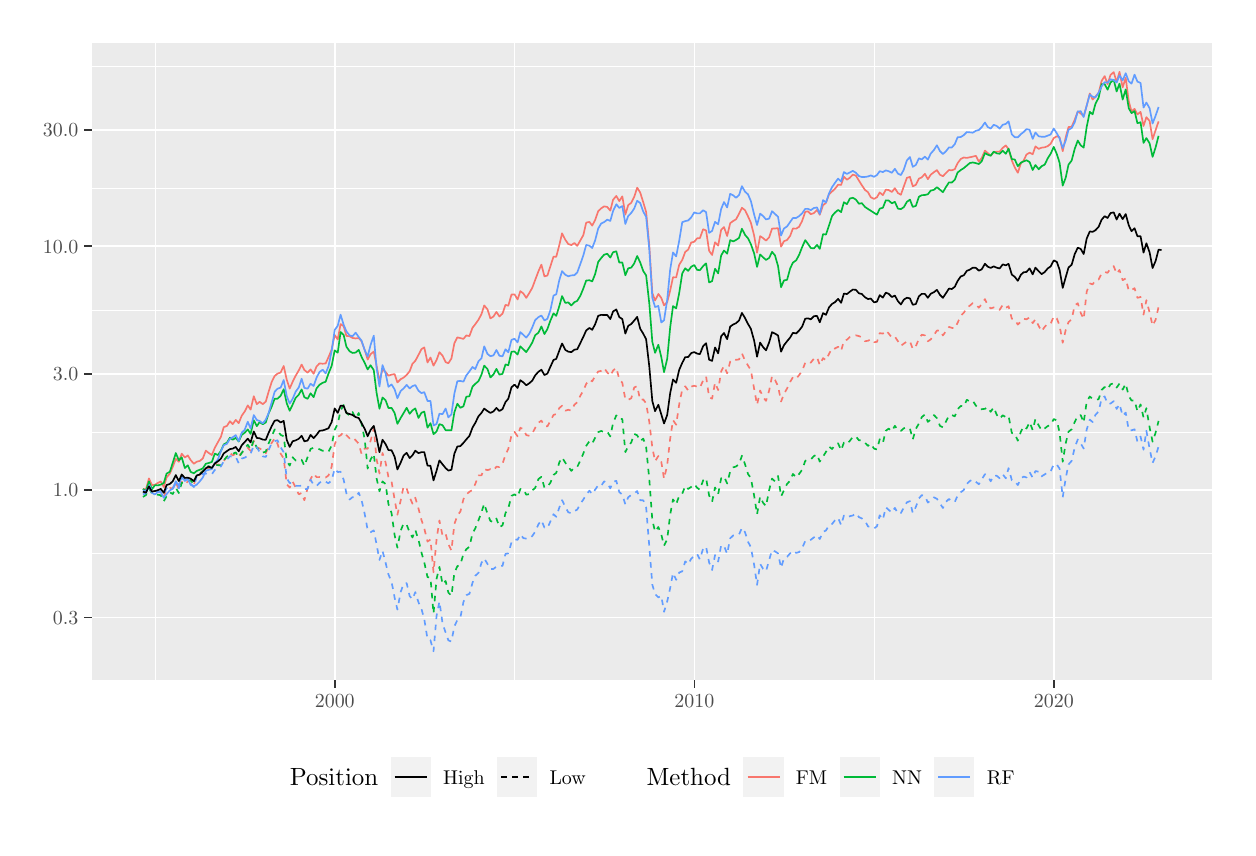
\begin{tikzpicture}[x=1pt,y=1pt]
\definecolor{fillColor}{RGB}{255,255,255}
\path[use as bounding box,fill=fillColor,fill opacity=0.00] (0,0) rectangle (433.62,289.08);
\begin{scope}
\path[clip] (  0.00,  0.00) rectangle (433.62,289.08);
\definecolor{drawColor}{RGB}{255,255,255}
\definecolor{fillColor}{RGB}{255,255,255}

\path[draw=drawColor,line width= 0.6pt,line join=round,line cap=round,fill=fillColor] (  0.00,  0.00) rectangle (433.62,289.08);
\end{scope}
\begin{scope}
\path[clip] ( 23.25, 53.26) rectangle (428.12,283.58);
\definecolor{fillColor}{gray}{0.92}

\path[fill=fillColor] ( 23.25, 53.26) rectangle (428.12,283.58);
\definecolor{drawColor}{RGB}{255,255,255}

\path[draw=drawColor,line width= 0.3pt,line join=round] ( 23.25, 98.94) --
	(428.12, 98.94);

\path[draw=drawColor,line width= 0.3pt,line join=round] ( 23.25,142.99) --
	(428.12,142.99);

\path[draw=drawColor,line width= 0.3pt,line join=round] ( 23.25,187.05) --
	(428.12,187.05);

\path[draw=drawColor,line width= 0.3pt,line join=round] ( 23.25,231.10) --
	(428.12,231.10);

\path[draw=drawColor,line width= 0.3pt,line join=round] ( 23.25,275.16) --
	(428.12,275.16);

\path[draw=drawColor,line width= 0.3pt,line join=round] ( 46.01, 53.26) --
	( 46.01,283.58);

\path[draw=drawColor,line width= 0.3pt,line join=round] (175.94, 53.26) --
	(175.94,283.58);

\path[draw=drawColor,line width= 0.3pt,line join=round] (305.86, 53.26) --
	(305.86,283.58);

\path[draw=drawColor,line width= 0.6pt,line join=round] ( 23.25, 75.90) --
	(428.12, 75.90);

\path[draw=drawColor,line width= 0.6pt,line join=round] ( 23.25,121.97) --
	(428.12,121.97);

\path[draw=drawColor,line width= 0.6pt,line join=round] ( 23.25,164.01) --
	(428.12,164.01);

\path[draw=drawColor,line width= 0.6pt,line join=round] ( 23.25,210.08) --
	(428.12,210.08);

\path[draw=drawColor,line width= 0.6pt,line join=round] ( 23.25,252.12) --
	(428.12,252.12);

\path[draw=drawColor,line width= 0.6pt,line join=round] (110.97, 53.26) --
	(110.97,283.58);

\path[draw=drawColor,line width= 0.6pt,line join=round] (240.91, 53.26) --
	(240.91,283.58);

\path[draw=drawColor,line width= 0.6pt,line join=round] (370.80, 53.26) --
	(370.80,283.58);
\definecolor{drawColor}{RGB}{248,118,109}

\path[draw=drawColor,line width= 0.6pt,line join=round] ( 41.65,122.42) --
	( 42.72,122.18) --
	( 43.82,126.20) --
	( 44.89,123.83) --
	( 45.95,123.88) --
	( 47.09,124.60) --
	( 48.09,125.11) --
	( 49.19,123.09) --
	( 50.19,126.54) --
	( 51.36,127.93) --
	( 52.43,130.39) --
	( 53.53,133.30) --
	( 54.63,132.20) --
	( 55.66,135.15) --
	( 56.80,133.77) --
	( 57.87,134.50) --
	( 58.90,132.81) --
	( 60.07,131.50) --
	( 61.11,132.26) --
	( 62.14,132.48) --
	( 63.28,133.40) --
	( 64.38,136.24) --
	( 65.37,135.43) --
	( 66.55,134.64) --
	( 67.62,137.26) --
	( 68.72,139.26) --
	( 69.82,141.21) --
	( 70.85,144.73) --
	( 71.99,145.17) --
	( 73.09,146.86) --
	( 74.09,145.81) --
	( 75.19,147.34) --
	( 76.26,146.17) --
	( 77.33,148.82) --
	( 78.43,150.39) --
	( 79.53,152.61) --
	( 80.56,151.05) --
	( 81.70,155.90) --
	( 82.80,153.02) --
	( 83.80,153.87) --
	( 84.97,153.05) --
	( 86.04,153.95) --
	( 87.04,157.44) --
	( 88.17,161.04) --
	( 89.24,163.20) --
	( 90.27,164.06) --
	( 91.41,164.49) --
	( 92.51,166.83) --
	( 93.62,161.81) --
	( 94.68,158.66) --
	( 95.75,161.12) --
	( 96.85,163.33) --
	( 97.96,165.24) --
	( 98.99,167.33) --
	( 99.98,165.38) --
	(101.16,164.42) --
	(102.22,165.60) --
	(103.33,164.03) --
	(104.39,166.68) --
	(105.46,167.77) --
	(106.60,167.65) --
	(107.67,167.75) --
	(108.70,170.00) --
	(109.84,172.77) --
	(110.94,178.03) --
	(112.04,176.41) --
	(113.07,181.99) --
	(114.18,181.22) --
	(115.17,177.69) --
	(116.34,177.58) --
	(117.41,176.96) --
	(118.51,176.78) --
	(119.62,176.94) --
	(120.65,175.74) --
	(121.79,172.61) --
	(122.85,169.14) --
	(123.89,171.07) --
	(125.06,172.05) --
	(126.06,167.04) --
	(127.12,161.38) --
	(128.22,165.61) --
	(129.33,164.66) --
	(130.36,163.32) --
	(131.50,163.72) --
	(132.60,163.89) --
	(133.60,160.89) --
	(134.77,162.05) --
	(135.84,162.63) --
	(136.94,163.59) --
	(138.04,164.97) --
	(139.04,167.62) --
	(140.07,168.69) --
	(141.21,170.82) --
	(142.31,172.93) --
	(143.31,173.54) --
	(144.48,168.08) --
	(145.55,169.88) --
	(146.65,166.96) --
	(147.75,168.98) --
	(148.78,171.82) --
	(149.92,170.54) --
	(151.02,168.24) --
	(152.02,167.81) --
	(153.12,169.53) --
	(154.19,175.06) --
	(155.26,177.16) --
	(156.36,176.91) --
	(157.46,176.61) --
	(158.49,177.86) --
	(159.63,177.64) --
	(160.73,180.63) --
	(161.73,181.91) --
	(162.90,183.54) --
	(163.97,185.54) --
	(164.97,188.71) --
	(166.14,187.31) --
	(167.21,184.01) --
	(168.31,184.70) --
	(169.38,186.37) --
	(170.45,184.73) --
	(171.58,185.74) --
	(172.65,188.92) --
	(173.68,188.61) --
	(174.82,192.64) --
	(175.92,192.72) --
	(177.03,190.87) --
	(178.02,193.87) --
	(179.12,193.02) --
	(180.16,191.43) --
	(181.29,193.25) --
	(182.36,195.13) --
	(183.39,197.93) --
	(184.57,201.05) --
	(185.63,203.46) --
	(186.74,199.19) --
	(187.80,199.52) --
	(188.87,202.83) --
	(190.01,206.35) --
	(191.00,206.31) --
	(192.11,210.53) --
	(193.10,214.77) --
	(194.28,212.43) --
	(195.34,210.90) --
	(196.45,210.52) --
	(197.55,211.26) --
	(198.58,210.23) --
	(199.72,212.23) --
	(200.79,214.13) --
	(201.82,218.63) --
	(202.99,218.89) --
	(203.99,217.56) --
	(205.05,219.58) --
	(206.16,222.78) --
	(207.26,223.80) --
	(208.29,224.51) --
	(209.43,224.29) --
	(210.53,222.95) --
	(211.53,226.90) --
	(212.70,228.27) --
	(213.77,226.41) --
	(214.87,228.13) --
	(215.97,221.54) --
	(217.00,224.95) --
	(218.11,225.81) --
	(219.17,227.92) --
	(220.24,231.26) --
	(221.34,229.49) --
	(222.45,225.94) --
	(223.48,222.45) --
	(224.62,210.36) --
	(225.72,193.17) --
	(226.71,190.50) --
	(227.89,192.85) --
	(228.96,191.41) --
	(229.95,188.73) --
	(231.09,189.89) --
	(232.16,194.09) --
	(233.19,198.88) --
	(234.33,198.83) --
	(235.43,203.41) --
	(236.53,205.16) --
	(237.60,208.04) --
	(238.67,208.88) --
	(239.77,211.44) --
	(240.87,211.71) --
	(241.90,212.97) --
	(242.90,213.02) --
	(244.07,216.23) --
	(245.14,215.82) --
	(246.24,208.44) --
	(247.31,206.95) --
	(248.38,211.55) --
	(249.51,210.31) --
	(250.58,216.05) --
	(251.61,217.03) --
	(252.75,213.80) --
	(253.85,218.43) --
	(254.96,219.25) --
	(255.95,219.81) --
	(257.06,221.85) --
	(258.09,223.99) --
	(259.22,223.12) --
	(260.29,220.89) --
	(261.32,218.63) --
	(262.50,213.98) --
	(263.56,207.76) --
	(264.67,213.74) --
	(265.73,213.04) --
	(266.80,212.13) --
	(267.94,213.34) --
	(268.97,216.47) --
	(270.04,216.52) --
	(271.14,216.62) --
	(272.24,209.94) --
	(273.27,211.91) --
	(274.41,212.36) --
	(275.52,213.84) --
	(276.51,216.50) --
	(277.69,216.45) --
	(278.75,217.13) --
	(279.85,219.25) --
	(280.96,222.54) --
	(281.95,222.72) --
	(282.98,221.69) --
	(284.12,222.07) --
	(285.23,223.23) --
	(286.22,221.48) --
	(287.40,224.91) --
	(288.46,225.78) --
	(289.57,228.87) --
	(290.67,229.89) --
	(291.70,230.83) --
	(292.84,232.33) --
	(293.94,232.25) --
	(294.94,235.24) --
	(296.04,234.13) --
	(297.11,234.87) --
	(298.17,236.00) --
	(299.28,235.60) --
	(300.38,233.80) --
	(301.41,232.16) --
	(302.55,230.46) --
	(303.65,229.62) --
	(304.65,227.78) --
	(305.82,227.20) --
	(306.89,227.81) --
	(307.88,229.52) --
	(309.02,228.57) --
	(310.09,230.53) --
	(311.12,230.40) --
	(312.26,229.70) --
	(313.36,231.06) --
	(314.46,229.32) --
	(315.53,228.70) --
	(316.60,231.74) --
	(317.70,234.81) --
	(318.80,235.17) --
	(319.83,231.76) --
	(320.94,232.27) --
	(322.04,234.51) --
	(323.07,234.99) --
	(324.21,236.28) --
	(325.28,234.33) --
	(326.31,235.95) --
	(327.48,236.86) --
	(328.55,237.61) --
	(329.65,235.91) --
	(330.72,235.41) --
	(331.79,236.51) --
	(332.92,237.65) --
	(333.92,237.51) --
	(335.02,237.97) --
	(336.02,240.11) --
	(337.19,241.65) --
	(338.26,242.16) --
	(339.36,242.01) --
	(340.46,242.26) --
	(341.50,242.47) --
	(342.63,242.77) --
	(343.70,240.70) --
	(344.73,241.95) --
	(345.91,244.65) --
	(346.90,243.79) --
	(347.97,242.84) --
	(349.07,244.02) --
	(350.17,244.29) --
	(351.21,244.27) --
	(352.34,245.66) --
	(353.45,246.51) --
	(354.44,245.17) --
	(355.62,241.09) --
	(356.68,238.58) --
	(357.79,236.65) --
	(358.89,240.07) --
	(359.88,241.02) --
	(360.92,243.24) --
	(362.05,243.91) --
	(363.16,243.34) --
	(364.15,246.18) --
	(365.33,245.29) --
	(366.39,245.72) --
	(367.50,245.85) --
	(368.60,246.28) --
	(369.63,247.11) --
	(370.77,249.18) --
	(371.87,249.84) --
	(372.87,249.47) --
	(374.01,244.46) --
	(375.07,249.38) --
	(376.10,253.16) --
	(377.24,253.28) --
	(378.34,255.81) --
	(379.45,258.81) --
	(380.51,258.06) --
	(381.58,257.15) --
	(382.68,260.91) --
	(383.79,265.30) --
	(384.82,263.12) --
	(385.81,264.16) --
	(386.99,265.48) --
	(388.06,269.83) --
	(389.16,271.58) --
	(390.22,268.68) --
	(391.29,272.02) --
	(392.43,273.00) --
	(393.50,269.42) --
	(394.53,273.11) --
	(395.67,267.51) --
	(396.77,270.95) --
	(397.87,262.50) --
	(398.87,258.84) --
	(399.97,259.73) --
	(401.00,257.73) --
	(402.14,258.64) --
	(403.21,253.57) --
	(404.24,256.73) --
	(405.41,255.37) --
	(406.48,248.77) --
	(407.58,252.09) --
	(408.65,255.20);

\path[draw=drawColor,line width= 0.6pt,dash pattern=on 2pt off 2pt ,line join=round] ( 41.65,122.41) --
	( 42.72,121.90) --
	( 43.82,124.38) --
	( 44.89,121.72) --
	( 45.95,121.67) --
	( 47.09,121.36) --
	( 48.09,121.10) --
	( 49.19,119.56) --
	( 50.19,122.23) --
	( 51.36,122.73) --
	( 52.43,122.66) --
	( 53.53,124.87) --
	( 54.63,122.10) --
	( 55.66,124.94) --
	( 56.80,123.97) --
	( 57.87,125.15) --
	( 58.90,125.60) --
	( 60.07,124.01) --
	( 61.11,127.28) --
	( 62.14,127.43) --
	( 63.28,129.61) --
	( 64.38,130.16) --
	( 65.37,129.91) --
	( 66.55,130.03) --
	( 67.62,131.66) --
	( 68.72,131.09) --
	( 69.82,131.63) --
	( 70.85,132.53) --
	( 71.99,133.98) --
	( 73.09,135.45) --
	( 74.09,134.48) --
	( 75.19,135.16) --
	( 76.26,134.23) --
	( 77.33,135.50) --
	( 78.43,136.02) --
	( 79.53,137.27) --
	( 80.56,136.14) --
	( 81.70,139.77) --
	( 82.80,137.38) --
	( 83.80,137.06) --
	( 84.97,136.32) --
	( 86.04,135.32) --
	( 87.04,137.62) --
	( 88.17,139.01) --
	( 89.24,140.65) --
	( 90.27,138.73) --
	( 91.41,135.15) --
	( 92.51,133.43) --
	( 93.62,124.06) --
	( 94.68,122.89) --
	( 95.75,125.10) --
	( 96.85,122.84) --
	( 97.96,120.46) --
	( 98.99,120.94) --
	( 99.98,118.33) --
	(101.16,122.68) --
	(102.22,125.97) --
	(103.33,127.92) --
	(104.39,126.66) --
	(105.46,126.69) --
	(106.60,126.36) --
	(107.67,126.53) --
	(108.70,127.27) --
	(109.84,130.44) --
	(110.94,138.47) --
	(112.04,141.25) --
	(113.07,141.76) --
	(114.18,142.99) --
	(115.17,141.83) --
	(116.34,140.65) --
	(117.41,141.12) --
	(118.51,140.00) --
	(119.62,138.75) --
	(120.65,135.03) --
	(121.79,137.02) --
	(122.85,136.92) --
	(123.89,139.71) --
	(125.06,144.23) --
	(126.06,133.23) --
	(127.12,127.99) --
	(128.22,135.40) --
	(129.33,131.92) --
	(130.36,126.64) --
	(131.50,125.02) --
	(132.60,118.51) --
	(133.60,113.07) --
	(134.77,118.18) --
	(135.84,123.37) --
	(136.94,122.51) --
	(138.04,119.44) --
	(139.04,117.08) --
	(140.07,119.23) --
	(141.21,115.34) --
	(142.31,111.12) --
	(143.31,108.14) --
	(144.48,103.38) --
	(145.55,104.13) --
	(146.65, 92.28) --
	(147.75,104.16) --
	(148.78,111.00) --
	(149.92,105.49) --
	(151.02,106.23) --
	(152.02,102.46) --
	(153.12,100.13) --
	(154.19,109.69) --
	(155.26,112.79) --
	(156.36,114.23) --
	(157.46,118.69) --
	(158.49,120.40) --
	(159.63,121.37) --
	(160.73,122.03) --
	(161.73,124.17) --
	(162.90,127.30) --
	(163.97,127.31) --
	(164.97,129.60) --
	(166.14,129.18) --
	(167.21,129.55) --
	(168.31,129.09) --
	(169.38,130.43) --
	(170.45,130.32) --
	(171.58,131.46) --
	(172.65,134.72) --
	(173.68,136.88) --
	(174.82,141.77) --
	(175.92,143.02) --
	(177.03,141.41) --
	(178.02,144.51) --
	(179.12,143.99) --
	(180.16,141.86) --
	(181.29,141.58) --
	(182.36,142.48) --
	(183.39,144.49) --
	(184.57,146.34) --
	(185.63,147.09) --
	(186.74,145.15) --
	(187.80,145.02) --
	(188.87,146.92) --
	(190.01,149.16) --
	(191.00,149.49) --
	(192.11,151.65) --
	(193.10,152.46) --
	(194.28,150.68) --
	(195.34,151.00) --
	(196.45,150.71) --
	(197.55,152.83) --
	(198.58,153.71) --
	(199.72,156.13) --
	(200.79,157.88) --
	(201.82,160.36) --
	(202.99,161.90) --
	(203.99,161.27) --
	(205.05,163.20) --
	(206.16,164.83) --
	(207.26,165.07) --
	(208.29,166.09) --
	(209.43,164.51) --
	(210.53,163.25) --
	(211.53,165.18) --
	(212.70,166.19) --
	(213.77,162.03) --
	(214.87,160.77) --
	(215.97,154.73) --
	(217.00,154.61) --
	(218.11,155.17) --
	(219.17,159.08) --
	(220.24,159.54) --
	(221.34,154.47) --
	(222.45,154.76) --
	(223.48,153.26) --
	(224.62,146.65) --
	(225.72,137.32) --
	(226.71,132.39) --
	(227.89,134.30) --
	(228.96,132.18) --
	(229.95,126.05) --
	(231.09,131.08) --
	(232.16,140.53) --
	(233.19,147.26) --
	(234.33,145.61) --
	(235.43,153.01) --
	(236.53,158.38) --
	(237.60,159.48) --
	(238.67,158.00) --
	(239.77,159.38) --
	(240.87,159.69) --
	(241.90,159.36) --
	(242.90,158.94) --
	(244.07,161.61) --
	(245.14,163.03) --
	(246.24,155.54) --
	(247.31,155.00) --
	(248.38,160.80) --
	(249.51,158.11) --
	(250.58,164.84) --
	(251.61,166.84) --
	(252.75,164.20) --
	(253.85,168.39) --
	(254.96,169.37) --
	(255.95,169.05) --
	(257.06,169.19) --
	(258.09,171.39) --
	(259.22,168.75) --
	(260.29,166.99) --
	(261.32,165.33) --
	(262.50,158.60) --
	(263.56,152.81) --
	(264.67,157.96) --
	(265.73,155.59) --
	(266.80,154.22) --
	(267.94,157.99) --
	(268.97,163.16) --
	(270.04,161.81) --
	(271.14,159.60) --
	(272.24,153.97) --
	(273.27,156.74) --
	(274.41,158.70) --
	(275.52,161.06) --
	(276.51,162.77) --
	(277.69,162.23) --
	(278.75,163.53) --
	(279.85,165.07) --
	(280.96,167.99) --
	(281.95,168.55) --
	(282.98,168.03) --
	(284.12,169.51) --
	(285.23,169.97) --
	(286.22,167.19) --
	(287.40,169.68) --
	(288.46,168.91) --
	(289.57,171.18) --
	(290.67,173.30) --
	(291.70,173.14) --
	(292.84,173.78) --
	(293.94,172.31) --
	(294.94,175.95) --
	(296.04,176.32) --
	(297.11,177.32) --
	(298.17,177.48) --
	(299.28,177.90) --
	(300.38,177.64) --
	(301.41,177.15) --
	(302.55,175.78) --
	(303.65,175.95) --
	(304.65,176.49) --
	(305.82,175.42) --
	(306.89,175.55) --
	(307.88,178.72) --
	(309.02,178.51) --
	(310.09,179.67) --
	(311.12,178.56) --
	(312.26,177.08) --
	(313.36,177.42) --
	(314.46,175.77) --
	(315.53,174.10) --
	(316.60,174.92) --
	(317.70,175.66) --
	(318.80,175.78) --
	(319.83,172.96) --
	(320.94,173.98) --
	(322.04,176.63) --
	(323.07,178.14) --
	(324.21,177.88) --
	(325.28,175.76) --
	(326.31,176.42) --
	(327.48,178.04) --
	(328.55,179.61) --
	(329.65,179.71) --
	(330.72,177.87) --
	(331.79,179.40) --
	(332.92,180.96) --
	(333.92,180.62) --
	(335.02,180.40) --
	(336.02,182.42) --
	(337.19,185.03) --
	(338.26,186.05) --
	(339.36,187.85) --
	(340.46,188.64) --
	(341.50,189.54) --
	(342.63,189.07) --
	(343.70,187.89) --
	(344.73,189.16) --
	(345.91,190.98) --
	(346.90,188.73) --
	(347.97,187.62) --
	(349.07,188.00) --
	(350.17,187.98) --
	(351.21,187.12) --
	(352.34,188.91) --
	(353.45,187.83) --
	(354.44,188.42) --
	(355.62,183.91) --
	(356.68,183.56) --
	(357.79,181.78) --
	(358.89,182.94) --
	(359.88,183.89) --
	(360.92,183.69) --
	(362.05,184.37) --
	(363.16,182.30) --
	(364.15,183.71) --
	(365.33,181.30) --
	(366.39,179.35) --
	(367.50,180.98) --
	(368.60,182.06) --
	(369.63,182.05) --
	(370.77,184.75) --
	(371.87,184.03) --
	(372.87,181.42) --
	(374.01,175.24) --
	(375.07,179.75) --
	(376.10,182.68) --
	(377.24,183.70) --
	(378.34,188.72) --
	(379.45,189.51) --
	(380.51,186.05) --
	(381.58,183.80) --
	(382.68,193.70) --
	(383.79,196.65) --
	(384.82,196.32) --
	(385.81,197.80) --
	(386.99,198.09) --
	(388.06,200.25) --
	(389.16,200.82) --
	(390.22,200.48) --
	(391.29,202.15) --
	(392.43,202.91) --
	(393.50,200.18) --
	(394.53,201.53) --
	(395.67,197.82) --
	(396.77,198.44) --
	(397.87,194.04) --
	(398.87,194.26) --
	(399.97,194.94) --
	(401.00,191.44) --
	(402.14,191.77) --
	(403.21,185.39) --
	(404.24,190.63) --
	(405.41,186.08) --
	(406.48,181.41) --
	(407.58,183.56) --
	(408.65,188.22);
\definecolor{drawColor}{RGB}{0,186,56}

\path[draw=drawColor,line width= 0.6pt,line join=round] ( 41.65,122.40) --
	( 42.72,121.63) --
	( 43.82,125.13) --
	( 44.89,122.27) --
	( 45.95,123.71) --
	( 47.09,123.70) --
	( 48.09,123.96) --
	( 49.19,124.56) --
	( 50.19,127.96) --
	( 51.36,128.57) --
	( 52.43,131.88) --
	( 53.53,135.37) --
	( 54.63,132.73) --
	( 55.66,133.83) --
	( 56.80,129.94) --
	( 57.87,130.93) --
	( 58.90,128.56) --
	( 60.07,128.05) --
	( 61.11,128.92) --
	( 62.14,129.31) --
	( 63.28,129.82) --
	( 64.38,131.51) --
	( 65.37,131.76) --
	( 66.55,132.13) --
	( 67.62,135.18) --
	( 68.72,134.62) --
	( 69.82,136.15) --
	( 70.85,138.49) --
	( 71.99,139.11) --
	( 73.09,140.92) --
	( 74.09,140.17) --
	( 75.19,140.88) --
	( 76.26,139.54) --
	( 77.33,141.90) --
	( 78.43,142.72) --
	( 79.53,143.90) --
	( 80.56,142.28) --
	( 81.70,147.25) --
	( 82.80,145.09) --
	( 83.80,146.55) --
	( 84.97,145.79) --
	( 86.04,146.42) --
	( 87.04,149.64) --
	( 88.17,152.13) --
	( 89.24,155.00) --
	( 90.27,155.01) --
	( 91.41,156.05) --
	( 92.51,158.43) --
	( 93.62,153.32) --
	( 94.68,150.65) --
	( 95.75,152.89) --
	( 96.85,155.36) --
	( 97.96,156.44) --
	( 98.99,158.36) --
	( 99.98,155.54) --
	(101.16,154.98) --
	(102.22,156.96) --
	(103.33,155.56) --
	(104.39,158.74) --
	(105.46,160.04) --
	(106.60,160.76) --
	(107.67,161.13) --
	(108.70,164.11) --
	(109.84,166.87) --
	(110.94,172.47) --
	(112.04,171.62) --
	(113.07,179.10) --
	(114.18,178.04) --
	(115.17,173.81) --
	(116.34,172.14) --
	(117.41,171.54) --
	(118.51,171.67) --
	(119.62,172.66) --
	(120.65,170.13) --
	(121.79,167.92) --
	(122.85,165.57) --
	(123.89,167.09) --
	(125.06,165.32) --
	(126.06,157.22) --
	(127.12,151.37) --
	(128.22,155.44) --
	(129.33,154.45) --
	(130.36,151.64) --
	(131.50,151.69) --
	(132.60,149.84) --
	(133.60,145.90) --
	(134.77,148.04) --
	(135.84,149.82) --
	(136.94,151.72) --
	(138.04,149.55) --
	(139.04,150.79) --
	(140.07,151.49) --
	(141.21,148.05) --
	(142.31,149.94) --
	(143.31,150.37) --
	(144.48,144.54) --
	(145.55,146.16) --
	(146.65,142.17) --
	(147.75,143.17) --
	(148.78,145.80) --
	(149.92,145.43) --
	(151.02,143.62) --
	(152.02,143.61) --
	(153.12,143.59) --
	(154.19,150.12) --
	(155.26,153.19) --
	(156.36,151.71) --
	(157.46,152.28) --
	(158.49,155.71) --
	(159.63,155.89) --
	(160.73,159.35) --
	(161.73,160.38) --
	(162.90,161.35) --
	(163.97,163.68) --
	(164.97,166.97) --
	(166.14,165.73) --
	(167.21,162.69) --
	(168.31,163.77) --
	(169.38,165.79) --
	(170.45,163.71) --
	(171.58,163.98) --
	(172.65,167.39) --
	(173.68,167.09) --
	(174.82,171.98) --
	(175.92,172.06) --
	(177.03,170.96) --
	(178.02,173.94) --
	(179.12,172.85) --
	(180.16,171.84) --
	(181.29,173.54) --
	(182.36,175.35) --
	(183.39,177.96) --
	(184.57,178.85) --
	(185.63,181.12) --
	(186.74,178.37) --
	(187.80,180.18) --
	(188.87,183.19) --
	(190.01,185.84) --
	(191.00,184.94) --
	(192.11,188.48) --
	(193.10,192.08) --
	(194.28,189.62) --
	(195.34,189.81) --
	(196.45,188.71) --
	(197.55,189.87) --
	(198.58,190.36) --
	(199.72,192.24) --
	(200.79,194.85) --
	(201.82,197.70) --
	(202.99,197.82) --
	(203.99,197.37) --
	(205.05,200.03) --
	(206.16,204.45) --
	(207.26,205.85) --
	(208.29,207.04) --
	(209.43,207.39) --
	(210.53,206.00) --
	(211.53,207.93) --
	(212.70,208.27) --
	(213.77,204.19) --
	(214.87,204.25) --
	(215.97,199.60) --
	(217.00,202.11) --
	(218.11,202.37) --
	(219.17,203.90) --
	(220.24,206.57) --
	(221.34,204.23) --
	(222.45,201.10) --
	(223.48,199.58) --
	(224.62,189.44) --
	(225.72,175.53) --
	(226.71,171.57) --
	(227.89,174.50) --
	(228.96,170.03) --
	(229.95,164.61) --
	(231.09,169.38) --
	(232.16,180.72) --
	(233.19,188.47) --
	(234.33,187.64) --
	(235.43,193.22) --
	(236.53,200.31) --
	(237.60,202.13) --
	(238.67,201.20) --
	(239.77,202.69) --
	(240.87,203.31) --
	(241.90,201.56) --
	(242.90,201.44) --
	(244.07,202.91) --
	(245.14,203.91) --
	(246.24,197.01) --
	(247.31,197.49) --
	(248.38,201.98) --
	(249.51,200.29) --
	(250.58,206.74) --
	(251.61,208.54) --
	(252.75,207.40) --
	(253.85,212.31) --
	(254.96,211.84) --
	(255.95,212.35) --
	(257.06,213.13) --
	(258.09,216.42) --
	(259.22,214.20) --
	(260.29,212.95) --
	(261.32,210.87) --
	(262.50,207.52) --
	(263.56,202.63) --
	(264.67,207.11) --
	(265.73,206.09) --
	(266.80,205.16) --
	(267.94,205.87) --
	(268.97,208.09) --
	(270.04,206.78) --
	(271.14,202.95) --
	(272.24,195.30) --
	(273.27,197.73) --
	(274.41,197.98) --
	(275.52,202.06) --
	(276.51,204.18) --
	(277.69,205.00) --
	(278.75,206.96) --
	(279.85,209.78) --
	(280.96,212.30) --
	(281.95,210.97) --
	(282.98,209.45) --
	(284.12,209.32) --
	(285.23,210.58) --
	(286.22,209.14) --
	(287.40,214.46) --
	(288.46,214.33) --
	(289.57,217.62) --
	(290.67,221.05) --
	(291.70,222.24) --
	(292.84,223.22) --
	(293.94,222.44) --
	(294.94,226.00) --
	(296.04,225.31) --
	(297.11,227.35) --
	(298.17,227.61) --
	(299.28,226.95) --
	(300.38,225.45) --
	(301.41,225.68) --
	(302.55,224.31) --
	(303.65,223.57) --
	(304.65,222.93) --
	(305.82,222.18) --
	(306.89,221.50) --
	(307.88,223.68) --
	(309.02,224.00) --
	(310.09,226.69) --
	(311.12,226.63) --
	(312.26,225.61) --
	(313.36,226.14) --
	(314.46,223.69) --
	(315.53,223.50) --
	(316.60,224.22) --
	(317.70,226.14) --
	(318.80,226.93) --
	(319.83,224.30) --
	(320.94,224.67) --
	(322.04,227.97) --
	(323.07,228.55) --
	(324.21,228.62) --
	(325.28,228.88) --
	(326.31,230.20) --
	(327.48,230.48) --
	(328.55,231.45) --
	(329.65,230.53) --
	(330.72,229.62) --
	(331.79,231.45) --
	(332.92,233.19) --
	(333.92,233.11) --
	(335.02,234.13) --
	(336.02,236.73) --
	(337.19,237.65) --
	(338.26,238.33) --
	(339.36,239.25) --
	(340.46,240.18) --
	(341.50,240.36) --
	(342.63,240.13) --
	(343.70,239.80) --
	(344.73,240.76) --
	(345.91,243.77) --
	(346.90,243.20) --
	(347.97,242.79) --
	(349.07,244.29) --
	(350.17,243.67) --
	(351.21,243.51) --
	(352.34,244.62) --
	(353.45,243.51) --
	(354.44,245.34) --
	(355.62,241.56) --
	(356.68,241.45) --
	(357.79,239.02) --
	(358.89,240.29) --
	(359.88,240.75) --
	(360.92,241.17) --
	(362.05,240.51) --
	(363.16,237.65) --
	(364.15,239.44) --
	(365.33,237.91) --
	(366.39,239.03) --
	(367.50,239.58) --
	(368.60,241.88) --
	(369.63,243.49) --
	(370.77,245.99) --
	(371.87,243.43) --
	(372.87,240.29) --
	(374.01,232.02) --
	(375.07,234.80) --
	(376.10,239.57) --
	(377.24,241.07) --
	(378.34,245.27) --
	(379.45,248.29) --
	(380.51,246.56) --
	(381.58,245.74) --
	(382.68,253.25) --
	(383.79,258.65) --
	(384.82,257.77) --
	(385.81,261.49) --
	(386.99,263.79) --
	(388.06,268.62) --
	(389.16,268.71) --
	(390.22,266.66) --
	(391.29,269.27) --
	(392.43,270.25) --
	(393.50,266.01) --
	(394.53,268.86) --
	(395.67,263.11) --
	(396.77,266.76) --
	(397.87,259.97) --
	(398.87,258.21) --
	(399.97,258.95) --
	(401.00,254.56) --
	(402.14,254.90) --
	(403.21,247.45) --
	(404.24,249.18) --
	(405.41,247.27) --
	(406.48,242.38) --
	(407.58,245.85) --
	(408.65,249.99);

\path[draw=drawColor,line width= 0.6pt,dash pattern=on 2pt off 2pt ,line join=round] ( 41.65,119.52) --
	( 42.72,120.16) --
	( 43.82,122.66) --
	( 44.89,120.78) --
	( 45.95,120.42) --
	( 47.09,120.31) --
	( 48.09,120.10) --
	( 49.19,117.89) --
	( 50.19,119.82) --
	( 51.36,121.17) --
	( 52.43,120.57) --
	( 53.53,122.79) --
	( 54.63,120.91) --
	( 55.66,124.61) --
	( 56.80,124.73) --
	( 57.87,125.20) --
	( 58.90,125.47) --
	( 60.07,124.07) --
	( 61.11,127.99) --
	( 62.14,127.83) --
	( 63.28,128.79) --
	( 64.38,130.36) --
	( 65.37,130.66) --
	( 66.55,129.83) --
	( 67.62,131.13) --
	( 68.72,130.99) --
	( 69.82,130.89) --
	( 70.85,132.70) --
	( 71.99,134.11) --
	( 73.09,134.59) --
	( 74.09,135.07) --
	( 75.19,135.60) --
	( 76.26,133.81) --
	( 77.33,135.35) --
	( 78.43,137.12) --
	( 79.53,138.34) --
	( 80.56,136.74) --
	( 81.70,140.04) --
	( 82.80,137.22) --
	( 83.80,136.69) --
	( 84.97,135.55) --
	( 86.04,135.87) --
	( 87.04,138.77) --
	( 88.17,141.37) --
	( 89.24,143.87) --
	( 90.27,143.66) --
	( 91.41,141.93) --
	( 92.51,141.41) --
	( 93.62,132.50) --
	( 94.68,130.81) --
	( 95.75,133.83) --
	( 96.85,132.68) --
	( 97.96,132.51) --
	( 98.99,132.95) --
	( 99.98,130.73) --
	(101.16,133.91) --
	(102.22,136.85) --
	(103.33,137.29) --
	(104.39,137.12) --
	(105.46,136.73) --
	(106.60,136.19) --
	(107.67,136.29) --
	(108.70,135.84) --
	(109.84,138.05) --
	(110.94,143.77) --
	(112.04,145.88) --
	(113.07,150.72) --
	(114.18,152.71) --
	(115.17,149.86) --
	(116.34,148.86) --
	(117.41,150.19) --
	(118.51,147.80) --
	(119.62,149.85) --
	(120.65,145.97) --
	(121.79,140.26) --
	(122.85,129.76) --
	(123.89,132.97) --
	(125.06,135.08) --
	(126.06,126.35) --
	(127.12,121.55) --
	(128.22,125.12) --
	(129.33,124.17) --
	(130.36,116.89) --
	(131.50,113.60) --
	(132.60,105.68) --
	(133.60,101.17) --
	(134.77,107.25) --
	(135.84,109.96) --
	(136.94,109.49) --
	(138.04,106.68) --
	(139.04,104.87) --
	(140.07,107.56) --
	(141.21,104.07) --
	(142.31, 99.36) --
	(143.31, 95.85) --
	(144.48, 90.53) --
	(145.55, 90.34) --
	(146.65, 77.35) --
	(147.75, 89.90) --
	(148.78, 94.25) --
	(149.92, 87.94) --
	(151.02, 89.14) --
	(152.02, 84.94) --
	(153.12, 83.81) --
	(154.19, 92.07) --
	(155.26, 94.48) --
	(156.36, 95.10) --
	(157.46, 98.93) --
	(158.49,100.60) --
	(159.63,101.54) --
	(160.73,106.32) --
	(161.73,108.12) --
	(162.90,111.07) --
	(163.97,113.95) --
	(164.97,117.09) --
	(166.14,113.43) --
	(167.21,110.84) --
	(168.31,110.38) --
	(169.38,111.72) --
	(170.45,108.61) --
	(171.58,109.23) --
	(172.65,113.67) --
	(173.68,115.42) --
	(174.82,119.89) --
	(175.92,120.46) --
	(177.03,119.57) --
	(178.02,122.38) --
	(179.12,122.31) --
	(180.16,120.32) --
	(181.29,120.54) --
	(182.36,121.90) --
	(183.39,122.77) --
	(184.57,125.98) --
	(185.63,126.76) --
	(186.74,122.83) --
	(187.80,123.19) --
	(188.87,124.64) --
	(190.01,127.46) --
	(191.00,128.21) --
	(192.11,132.02) --
	(193.10,133.78) --
	(194.28,131.86) --
	(195.34,130.49) --
	(196.45,128.93) --
	(197.55,130.17) --
	(198.58,130.35) --
	(199.72,132.67) --
	(200.79,135.23) --
	(201.82,137.94) --
	(202.99,139.68) --
	(203.99,138.84) --
	(205.05,140.91) --
	(206.16,142.94) --
	(207.26,143.35) --
	(208.29,142.88) --
	(209.43,143.09) --
	(210.53,141.37) --
	(211.53,146.22) --
	(212.70,148.99) --
	(213.77,147.59) --
	(214.87,147.69) --
	(215.97,135.70) --
	(217.00,137.78) --
	(218.11,139.21) --
	(219.17,142.31) --
	(220.24,141.79) --
	(221.34,139.71) --
	(222.45,140.57) --
	(223.48,137.51) --
	(224.62,125.87) --
	(225.72,111.08) --
	(226.71,106.99) --
	(227.89,108.65) --
	(228.96,105.95) --
	(229.95,101.89) --
	(231.09,104.18) --
	(232.16,113.07) --
	(233.19,118.62) --
	(234.33,116.79) --
	(235.43,119.99) --
	(236.53,120.67) --
	(237.60,123.46) --
	(238.67,122.40) --
	(239.77,123.14) --
	(240.87,124.14) --
	(241.90,122.81) --
	(242.90,122.12) --
	(244.07,125.50) --
	(245.14,126.30) --
	(246.24,120.02) --
	(247.31,117.75) --
	(248.38,122.92) --
	(249.51,120.52) --
	(250.58,126.25) --
	(251.61,126.95) --
	(252.75,124.38) --
	(253.85,128.74) --
	(254.96,130.20) --
	(255.95,130.51) --
	(257.06,131.40) --
	(258.09,134.41) --
	(259.22,131.31) --
	(260.29,127.81) --
	(261.32,126.32) --
	(262.50,119.99) --
	(263.56,113.21) --
	(264.67,119.62) --
	(265.73,117.40) --
	(266.80,116.18) --
	(267.94,122.00) --
	(268.97,126.13) --
	(270.04,125.15) --
	(271.14,127.08) --
	(272.24,119.72) --
	(273.27,121.86) --
	(274.41,124.22) --
	(275.52,125.40) --
	(276.51,127.82) --
	(277.69,126.56) --
	(278.75,127.79) --
	(279.85,129.33) --
	(280.96,132.52) --
	(281.95,133.01) --
	(282.98,133.04) --
	(284.12,134.31) --
	(285.23,134.86) --
	(286.22,132.28) --
	(287.40,134.10) --
	(288.46,135.78) --
	(289.57,137.69) --
	(290.67,136.83) --
	(291.70,138.26) --
	(292.84,138.89) --
	(293.94,136.37) --
	(294.94,139.15) --
	(296.04,138.69) --
	(297.11,139.81) --
	(298.17,141.19) --
	(299.28,141.39) --
	(300.38,139.95) --
	(301.41,140.00) --
	(302.55,139.13) --
	(303.65,137.95) --
	(304.65,138.78) --
	(305.82,136.96) --
	(306.89,136.68) --
	(307.88,140.34) --
	(309.02,139.01) --
	(310.09,143.43) --
	(311.12,144.19) --
	(312.26,143.27) --
	(313.36,145.22) --
	(314.46,143.60) --
	(315.53,143.37) --
	(316.60,144.31) --
	(317.70,144.62) --
	(318.80,144.23) --
	(319.83,140.31) --
	(320.94,144.12) --
	(322.04,146.02) --
	(323.07,148.34) --
	(324.21,149.30) --
	(325.28,146.64) --
	(326.31,147.46) --
	(327.48,149.08) --
	(328.55,147.99) --
	(329.65,145.19) --
	(330.72,144.65) --
	(331.79,146.70) --
	(332.92,148.96) --
	(333.92,149.08) --
	(335.02,148.64) --
	(336.02,151.23) --
	(337.19,152.38) --
	(338.26,152.21) --
	(339.36,154.60) --
	(340.46,154.02) --
	(341.50,154.25) --
	(342.63,152.52) --
	(343.70,151.20) --
	(344.73,151.21) --
	(345.91,151.35) --
	(346.90,151.95) --
	(347.97,150.27) --
	(349.07,151.90) --
	(350.17,149.20) --
	(351.21,147.77) --
	(352.34,149.00) --
	(353.45,148.36) --
	(354.44,148.79) --
	(355.62,142.60) --
	(356.68,142.37) --
	(357.79,139.83) --
	(358.89,143.09) --
	(359.88,145.01) --
	(360.92,144.24) --
	(362.05,146.55) --
	(363.16,143.68) --
	(364.15,147.65) --
	(365.33,145.35) --
	(366.39,143.57) --
	(367.50,144.27) --
	(368.60,145.12) --
	(369.63,145.53) --
	(370.77,147.66) --
	(371.87,147.15) --
	(372.87,142.79) --
	(374.01,132.22) --
	(375.07,138.82) --
	(376.10,143.08) --
	(377.24,143.96) --
	(378.34,146.57) --
	(379.45,148.88) --
	(380.51,149.09) --
	(381.58,146.39) --
	(382.68,153.93) --
	(383.79,155.80) --
	(384.82,154.88) --
	(385.81,154.62) --
	(386.99,154.83) --
	(388.06,158.17) --
	(389.16,159.23) --
	(390.22,158.37) --
	(391.29,160.22) --
	(392.43,160.59) --
	(393.50,159.03) --
	(394.53,160.47) --
	(395.67,158.31) --
	(396.77,160.41) --
	(397.87,155.99) --
	(398.87,154.34) --
	(399.97,154.39) --
	(401.00,150.45) --
	(402.14,152.95) --
	(403.21,148.22) --
	(404.24,151.58) --
	(405.41,144.60) --
	(406.48,139.48) --
	(407.58,142.78) --
	(408.65,146.98);
\definecolor{drawColor}{RGB}{97,156,255}

\path[draw=drawColor,line width= 0.6pt,line join=round] ( 41.65,120.42) --
	( 42.72,120.87) --
	( 43.82,123.34) --
	( 44.89,120.99) --
	( 45.95,120.41) --
	( 47.09,121.38) --
	( 48.09,121.26) --
	( 49.19,119.19) --
	( 50.19,120.51) --
	( 51.36,121.88) --
	( 52.43,122.50) --
	( 53.53,125.16) --
	( 54.63,123.42) --
	( 55.66,127.08) --
	( 56.80,125.27) --
	( 57.87,126.11) --
	( 58.90,123.85) --
	( 60.07,123.39) --
	( 61.11,123.98) --
	( 62.14,125.08) --
	( 63.28,126.51) --
	( 64.38,129.00) --
	( 65.37,129.29) --
	( 66.55,129.58) --
	( 67.62,131.71) --
	( 68.72,133.00) --
	( 69.82,135.98) --
	( 70.85,138.21) --
	( 71.99,138.69) --
	( 73.09,140.50) --
	( 74.09,141.09) --
	( 75.19,141.84) --
	( 76.26,139.65) --
	( 77.33,142.75) --
	( 78.43,143.77) --
	( 79.53,146.68) --
	( 80.56,144.25) --
	( 81.70,149.10) --
	( 82.80,147.30) --
	( 83.80,146.98) --
	( 84.97,146.09) --
	( 86.04,147.45) --
	( 87.04,149.72) --
	( 88.17,153.70) --
	( 89.24,157.51) --
	( 90.27,158.61) --
	( 91.41,159.01) --
	( 92.51,161.75) --
	( 93.62,155.93) --
	( 94.68,153.26) --
	( 95.75,154.96) --
	( 96.85,157.59) --
	( 97.96,159.08) --
	( 98.99,162.22) --
	( 99.98,158.92) --
	(101.16,158.63) --
	(102.22,160.41) --
	(103.33,159.60) --
	(104.39,162.64) --
	(105.46,164.67) --
	(106.60,165.47) --
	(107.67,164.17) --
	(108.70,166.68) --
	(109.84,172.24) --
	(110.94,179.85) --
	(112.04,181.36) --
	(113.07,185.38) --
	(114.18,181.71) --
	(115.17,179.32) --
	(116.34,177.86) --
	(117.41,177.61) --
	(118.51,178.86) --
	(119.62,177.28) --
	(120.65,176.00) --
	(121.79,172.55) --
	(122.85,170.26) --
	(123.89,174.38) --
	(125.06,177.80) --
	(126.06,166.24) --
	(127.12,159.42) --
	(128.22,167.15) --
	(129.33,164.13) --
	(130.36,159.31) --
	(131.50,160.15) --
	(132.60,158.36) --
	(133.60,155.15) --
	(134.77,157.78) --
	(135.84,158.72) --
	(136.94,159.99) --
	(138.04,158.71) --
	(139.04,159.54) --
	(140.07,159.94) --
	(141.21,157.89) --
	(142.31,157.03) --
	(143.31,157.38) --
	(144.48,154.17) --
	(145.55,154.20) --
	(146.65,145.34) --
	(147.75,145.86) --
	(148.78,149.59) --
	(149.92,149.42) --
	(151.02,151.44) --
	(152.02,148.26) --
	(153.12,149.33) --
	(154.19,156.89) --
	(155.26,161.32) --
	(156.36,161.44) --
	(157.46,161.16) --
	(158.49,163.40) --
	(159.63,164.88) --
	(160.73,166.46) --
	(161.73,165.73) --
	(162.90,168.54) --
	(163.97,169.60) --
	(164.97,173.92) --
	(166.14,171.19) --
	(167.21,170.36) --
	(168.31,170.66) --
	(169.38,172.61) --
	(170.45,170.55) --
	(171.58,170.30) --
	(172.65,172.87) --
	(173.68,171.76) --
	(174.82,176.27) --
	(175.92,176.67) --
	(177.03,175.36) --
	(178.02,179.08) --
	(179.12,178.06) --
	(180.16,177.08) --
	(181.29,178.53) --
	(182.36,180.84) --
	(183.39,183.41) --
	(184.57,184.49) --
	(185.63,185.07) --
	(186.74,183.27) --
	(187.80,183.88) --
	(188.87,186.94) --
	(190.01,192.28) --
	(191.00,192.75) --
	(192.11,197.89) --
	(193.10,201.09) --
	(194.28,199.78) --
	(195.34,199.24) --
	(196.45,199.57) --
	(197.55,199.64) --
	(198.58,200.62) --
	(199.72,203.73) --
	(200.79,206.81) --
	(201.82,210.56) --
	(202.99,210.28) --
	(203.99,209.46) --
	(205.05,212.20) --
	(206.16,216.52) --
	(207.26,218.34) --
	(208.29,218.81) --
	(209.43,219.70) --
	(210.53,219.24) --
	(211.53,222.83) --
	(212.70,225.26) --
	(213.77,223.94) --
	(214.87,224.61) --
	(215.97,218.15) --
	(217.00,221.03) --
	(218.11,222.15) --
	(219.17,223.72) --
	(220.24,226.53) --
	(221.34,225.72) --
	(222.45,222.58) --
	(223.48,220.74) --
	(224.62,209.03) --
	(225.72,191.45) --
	(226.71,188.14) --
	(227.89,188.52) --
	(228.96,182.55) --
	(229.95,183.35) --
	(231.09,190.75) --
	(232.16,201.65) --
	(233.19,207.85) --
	(234.33,206.43) --
	(235.43,212.09) --
	(236.53,218.81) --
	(237.60,219.17) --
	(238.67,219.42) --
	(239.77,220.52) --
	(240.87,222.33) --
	(241.90,221.96) --
	(242.90,221.97) --
	(244.07,223.10) --
	(245.14,222.43) --
	(246.24,214.94) --
	(247.31,215.65) --
	(248.38,218.90) --
	(249.51,218.03) --
	(250.58,223.54) --
	(251.61,226.06) --
	(252.75,224.12) --
	(253.85,229.06) --
	(254.96,228.47) --
	(255.95,227.60) --
	(257.06,228.60) --
	(258.09,231.81) --
	(259.22,229.80) --
	(260.29,228.85) --
	(261.32,226.45) --
	(262.50,221.59) --
	(263.56,217.76) --
	(264.67,221.87) --
	(265.73,221.03) --
	(266.80,219.78) --
	(267.94,220.09) --
	(268.97,222.75) --
	(270.04,221.76) --
	(271.14,220.76) --
	(272.24,213.97) --
	(273.27,216.50) --
	(274.41,217.27) --
	(275.52,218.87) --
	(276.51,220.30) --
	(277.69,220.31) --
	(278.75,220.98) --
	(279.85,221.99) --
	(280.96,223.59) --
	(281.95,223.62) --
	(282.98,223.14) --
	(284.12,223.92) --
	(285.23,224.12) --
	(286.22,221.76) --
	(287.40,226.76) --
	(288.46,225.92) --
	(289.57,229.22) --
	(290.67,231.47) --
	(291.70,232.98) --
	(292.84,234.54) --
	(293.94,233.46) --
	(294.94,236.91) --
	(296.04,236.22) --
	(297.11,236.77) --
	(298.17,237.34) --
	(299.28,236.63) --
	(300.38,235.44) --
	(301.41,235.10) --
	(302.55,235.14) --
	(303.65,235.31) --
	(304.65,235.69) --
	(305.82,235.19) --
	(306.89,235.83) --
	(307.88,237.22) --
	(309.02,236.90) --
	(310.09,237.52) --
	(311.12,237.20) --
	(312.26,236.64) --
	(313.36,238.07) --
	(314.46,236.36) --
	(315.53,235.81) --
	(316.60,237.80) --
	(317.70,241.10) --
	(318.80,242.35) --
	(319.83,238.80) --
	(320.94,239.47) --
	(322.04,241.88) --
	(323.07,241.45) --
	(324.21,242.49) --
	(325.28,241.39) --
	(326.31,243.57) --
	(327.48,244.89) --
	(328.55,246.58) --
	(329.65,244.47) --
	(330.72,243.41) --
	(331.79,244.39) --
	(332.92,245.83) --
	(333.92,245.76) --
	(335.02,246.99) --
	(336.02,249.47) --
	(337.19,249.57) --
	(338.26,250.26) --
	(339.36,251.35) --
	(340.46,251.26) --
	(341.50,251.12) --
	(342.63,251.82) --
	(343.70,252.10) --
	(344.73,253.10) --
	(345.91,254.82) --
	(346.90,253.18) --
	(347.97,252.63) --
	(349.07,253.97) --
	(350.17,253.56) --
	(351.21,252.60) --
	(352.34,253.99) --
	(353.45,254.31) --
	(354.44,255.21) --
	(355.62,250.55) --
	(356.68,249.51) --
	(357.79,249.46) --
	(358.89,250.59) --
	(359.88,251.37) --
	(360.92,252.42) --
	(362.05,252.17) --
	(363.16,248.89) --
	(364.15,251.19) --
	(365.33,249.82) --
	(366.39,249.66) --
	(367.50,249.65) --
	(368.60,250.07) --
	(369.63,250.47) --
	(370.77,252.64) --
	(371.87,250.92) --
	(372.87,249.08) --
	(374.01,245.58) --
	(375.07,248.19) --
	(376.10,252.18) --
	(377.24,252.81) --
	(378.34,254.88) --
	(379.45,258.78) --
	(380.51,258.89) --
	(381.58,256.78) --
	(382.68,260.94) --
	(383.79,264.93) --
	(384.82,264.11) --
	(385.81,263.85) --
	(386.99,265.61) --
	(388.06,267.85) --
	(389.16,269.38) --
	(390.22,269.20) --
	(391.29,270.44) --
	(392.43,270.13) --
	(393.50,269.27) --
	(394.53,271.82) --
	(395.67,270.02) --
	(396.77,272.62) --
	(397.87,269.69) --
	(398.87,268.84) --
	(399.97,272.10) --
	(401.00,269.58) --
	(402.14,269.11) --
	(403.21,260.22) --
	(404.24,262.01) --
	(405.41,259.94) --
	(406.48,254.46) --
	(407.58,257.27) --
	(408.65,260.42);

\path[draw=drawColor,line width= 0.6pt,dash pattern=on 2pt off 2pt ,line join=round] ( 41.65,121.87) --
	( 42.72,121.59) --
	( 43.82,124.14) --
	( 44.89,121.64) --
	( 45.95,121.62) --
	( 47.09,121.34) --
	( 48.09,121.60) --
	( 49.19,120.56) --
	( 50.19,122.57) --
	( 51.36,122.95) --
	( 52.43,122.43) --
	( 53.53,124.49) --
	( 54.63,122.56) --
	( 55.66,126.23) --
	( 56.80,125.91) --
	( 57.87,124.89) --
	( 58.90,124.29) --
	( 60.07,123.06) --
	( 61.11,127.16) --
	( 62.14,127.60) --
	( 63.28,127.81) --
	( 64.38,127.93) --
	( 65.37,127.91) --
	( 66.55,127.67) --
	( 67.62,129.29) --
	( 68.72,129.66) --
	( 69.82,130.52) --
	( 70.85,132.38) --
	( 71.99,132.93) --
	( 73.09,134.23) --
	( 74.09,134.05) --
	( 75.19,134.01) --
	( 76.26,131.65) --
	( 77.33,133.35) --
	( 78.43,133.71) --
	( 79.53,134.34) --
	( 80.56,135.13) --
	( 81.70,138.10) --
	( 82.80,137.40) --
	( 83.80,135.79) --
	( 84.97,134.17) --
	( 86.04,133.96) --
	( 87.04,136.37) --
	( 88.17,138.96) --
	( 89.24,139.66) --
	( 90.27,139.99) --
	( 91.41,137.46) --
	( 92.51,135.68) --
	( 93.62,126.20) --
	( 94.68,124.55) --
	( 95.75,124.54) --
	( 96.85,123.53) --
	( 97.96,123.50) --
	( 98.99,123.55) --
	( 99.98,122.28) --
	(101.16,122.44) --
	(102.22,125.77) --
	(103.33,123.83) --
	(104.39,123.46) --
	(105.46,124.61) --
	(106.60,125.40) --
	(107.67,125.01) --
	(108.70,124.44) --
	(109.84,125.53) --
	(110.94,129.71) --
	(112.04,128.51) --
	(113.07,128.62) --
	(114.18,125.72) --
	(115.17,120.82) --
	(116.34,118.59) --
	(117.41,119.45) --
	(118.51,119.36) --
	(119.62,121.05) --
	(120.65,118.39) --
	(121.79,113.32) --
	(122.85,107.56) --
	(123.89,106.73) --
	(125.06,107.44) --
	(126.06,102.43) --
	(127.12, 96.75) --
	(128.22,100.02) --
	(129.33, 95.75) --
	(130.36, 91.52) --
	(131.50, 88.81) --
	(132.60, 83.08) --
	(133.60, 78.82) --
	(134.77, 85.12) --
	(135.84, 88.13) --
	(136.94, 88.37) --
	(138.04, 83.65) --
	(139.04, 82.57) --
	(140.07, 85.11) --
	(141.21, 81.46) --
	(142.31, 78.99) --
	(143.31, 75.33) --
	(144.48, 68.12) --
	(145.55, 67.70) --
	(146.65, 63.73) --
	(147.75, 76.57) --
	(148.78, 81.73) --
	(149.92, 73.76) --
	(151.02, 70.54) --
	(152.02, 67.67) --
	(153.12, 67.29) --
	(154.19, 72.82) --
	(155.26, 74.98) --
	(156.36, 75.96) --
	(157.46, 81.53) --
	(158.49, 84.02) --
	(159.63, 84.50) --
	(160.73, 88.45) --
	(161.73, 91.00) --
	(162.90, 92.09) --
	(163.97, 95.66) --
	(164.97, 97.31) --
	(166.14, 95.32) --
	(167.21, 93.50) --
	(168.31, 93.49) --
	(169.38, 94.36) --
	(170.45, 94.39) --
	(171.58, 94.62) --
	(172.65, 98.92) --
	(173.68, 99.15) --
	(174.82,103.07) --
	(175.92,104.28) --
	(177.03,103.99) --
	(178.02,106.01) --
	(179.12,104.64) --
	(180.16,104.44) --
	(181.29,104.46) --
	(182.36,105.43) --
	(183.39,106.95) --
	(184.57,109.63) --
	(185.63,111.10) --
	(186.74,108.44) --
	(187.80,108.21) --
	(188.87,110.63) --
	(190.01,113.26) --
	(191.00,112.33) --
	(192.11,115.68) --
	(193.10,118.34) --
	(194.28,115.93) --
	(195.34,113.96) --
	(196.45,113.59) --
	(197.55,114.40) --
	(198.58,114.94) --
	(199.72,117.03) --
	(200.79,118.58) --
	(201.82,120.35) --
	(202.99,121.76) --
	(203.99,120.52) --
	(205.05,122.14) --
	(206.16,123.74) --
	(207.26,123.51) --
	(208.29,125.16) --
	(209.43,124.45) --
	(210.53,122.64) --
	(211.53,124.94) --
	(212.70,125.33) --
	(213.77,121.27) --
	(214.87,120.37) --
	(215.97,116.81) --
	(217.00,119.38) --
	(218.11,120.24) --
	(219.17,120.74) --
	(220.24,121.64) --
	(221.34,118.33) --
	(222.45,118.28) --
	(223.48,115.78) --
	(224.62,101.64) --
	(225.72, 87.77) --
	(226.71, 84.42) --
	(227.89, 83.21) --
	(228.96, 83.76) --
	(229.95, 78.00) --
	(231.09, 81.76) --
	(232.16, 86.55) --
	(233.19, 92.02) --
	(234.33, 89.56) --
	(235.43, 92.20) --
	(236.53, 92.61) --
	(237.60, 96.22) --
	(238.67, 95.21) --
	(239.77, 97.19) --
	(240.87, 98.20) --
	(241.90, 98.92) --
	(242.90, 96.93) --
	(244.07,100.90) --
	(245.14,101.54) --
	(246.24, 95.82) --
	(247.31, 93.10) --
	(248.38, 98.50) --
	(249.51, 96.15) --
	(250.58,102.02) --
	(251.61,101.89) --
	(252.75, 98.94) --
	(253.85,104.55) --
	(254.96,105.61) --
	(255.95,105.63) --
	(257.06,105.93) --
	(258.09,108.35) --
	(259.22,106.75) --
	(260.29,103.32) --
	(261.32,101.36) --
	(262.50, 95.02) --
	(263.56, 87.72) --
	(264.67, 95.34) --
	(265.73, 93.55) --
	(266.80, 92.63) --
	(267.94, 96.77) --
	(268.97,100.31) --
	(270.04, 99.83) --
	(271.14, 99.11) --
	(272.24, 93.87) --
	(273.27, 97.32) --
	(274.41, 97.88) --
	(275.52, 99.14) --
	(276.51,100.03) --
	(277.69, 99.29) --
	(278.75, 99.57) --
	(279.85,101.03) --
	(280.96,103.54) --
	(281.95,103.42) --
	(282.98,104.03) --
	(284.12,104.90) --
	(285.23,105.67) --
	(286.22,104.28) --
	(287.40,106.93) --
	(288.46,107.36) --
	(289.57,109.35) --
	(290.67,109.74) --
	(291.70,111.05) --
	(292.84,111.98) --
	(293.94,109.33) --
	(294.94,112.79) --
	(296.04,112.07) --
	(297.11,112.56) --
	(298.17,112.81) --
	(299.28,113.60) --
	(300.38,112.21) --
	(301.41,111.75) --
	(302.55,110.94) --
	(303.65,108.82) --
	(304.65,108.75) --
	(305.82,108.10) --
	(306.89,108.92) --
	(307.88,112.88) --
	(309.02,111.31) --
	(310.09,115.76) --
	(311.12,114.84) --
	(312.26,113.84) --
	(313.36,115.56) --
	(314.46,113.47) --
	(315.53,113.68) --
	(316.60,115.67) --
	(317.70,117.57) --
	(318.80,117.97) --
	(319.83,113.67) --
	(320.94,115.91) --
	(322.04,118.95) --
	(323.07,120.16) --
	(324.21,119.86) --
	(325.28,117.47) --
	(326.31,118.28) --
	(327.48,119.36) --
	(328.55,118.84) --
	(329.65,117.21) --
	(330.72,115.50) --
	(331.79,117.72) --
	(332.92,118.79) --
	(333.92,117.85) --
	(335.02,117.71) --
	(336.02,119.99) --
	(337.19,121.22) --
	(338.26,122.01) --
	(339.36,124.23) --
	(340.46,125.27) --
	(341.50,125.83) --
	(342.63,124.97) --
	(343.70,124.10) --
	(344.73,125.80) --
	(345.91,127.74) --
	(346.90,127.16) --
	(347.97,125.16) --
	(349.07,127.27) --
	(350.17,127.16) --
	(351.21,126.27) --
	(352.34,127.71) --
	(353.45,126.24) --
	(354.44,129.92) --
	(355.62,125.57) --
	(356.68,125.25) --
	(357.79,123.80) --
	(358.89,126.14) --
	(359.88,126.87) --
	(360.92,126.54) --
	(362.05,128.45) --
	(363.16,126.46) --
	(364.15,128.87) --
	(365.33,128.61) --
	(366.39,126.94) --
	(367.50,127.66) --
	(368.60,128.38) --
	(369.63,128.65) --
	(370.77,131.35) --
	(371.87,131.20) --
	(372.87,129.76) --
	(374.01,119.39) --
	(375.07,126.14) --
	(376.10,131.24) --
	(377.24,132.54) --
	(378.34,137.35) --
	(379.45,140.27) --
	(380.51,138.87) --
	(381.58,136.99) --
	(382.68,143.91) --
	(383.79,147.45) --
	(384.82,146.56) --
	(385.81,149.15) --
	(386.99,150.40) --
	(388.06,155.13) --
	(389.16,155.83) --
	(390.22,153.15) --
	(391.29,153.26) --
	(392.43,154.11) --
	(393.50,151.31) --
	(394.53,153.07) --
	(395.67,148.81) --
	(396.77,149.97) --
	(397.87,143.61) --
	(398.87,143.57) --
	(399.97,143.96) --
	(401.00,139.47) --
	(402.14,141.33) --
	(403.21,136.58) --
	(404.24,143.43) --
	(405.41,136.91) --
	(406.48,131.79) --
	(407.58,134.21) --
	(408.65,137.80);
\definecolor{drawColor}{RGB}{0,0,0}

\path[draw=drawColor,line width= 0.6pt,line join=round] ( 41.65,121.44) --
	( 42.72,121.05) --
	( 43.82,123.32) --
	( 44.89,121.45) --
	( 45.95,121.65) --
	( 47.09,121.97) --
	( 48.09,122.43) --
	( 49.19,120.99) --
	( 50.19,123.80) --
	( 51.36,124.20) --
	( 52.43,125.18) --
	( 53.53,127.42) --
	( 54.63,125.22) --
	( 55.66,127.62) --
	( 56.80,126.37) --
	( 57.87,126.47) --
	( 58.90,126.11) --
	( 60.07,125.22) --
	( 61.11,127.31) --
	( 62.14,127.58) --
	( 63.28,128.63) --
	( 64.38,129.87) --
	( 65.37,130.47) --
	( 66.55,129.99) --
	( 67.62,131.62) --
	( 68.72,132.34) --
	( 69.82,133.33) --
	( 70.85,135.23) --
	( 71.99,136.07) --
	( 73.09,136.80) --
	( 74.09,136.97) --
	( 75.19,137.59) --
	( 76.26,135.99) --
	( 77.33,138.17) --
	( 78.43,139.35) --
	( 79.53,140.59) --
	( 80.56,139.22) --
	( 81.70,143.17) --
	( 82.80,140.83) --
	( 83.80,140.71) --
	( 84.97,140.22) --
	( 86.04,140.17) --
	( 87.04,142.61) --
	( 88.17,145.07) --
	( 89.24,147.06) --
	( 90.27,147.27) --
	( 91.41,146.44) --
	( 92.51,146.98) --
	( 93.62,140.09) --
	( 94.68,137.58) --
	( 95.75,139.62) --
	( 96.85,139.96) --
	( 97.96,140.52) --
	( 98.99,141.61) --
	( 99.98,139.60) --
	(101.16,139.88) --
	(102.22,141.91) --
	(103.33,140.77) --
	(104.39,141.95) --
	(105.46,143.41) --
	(106.60,143.54) --
	(107.67,143.91) --
	(108.70,144.32) --
	(109.84,146.55) --
	(110.94,151.49) --
	(112.04,149.87) --
	(113.07,152.51) --
	(114.18,152.41) --
	(115.17,149.84) --
	(116.34,149.47) --
	(117.41,149.10) --
	(118.51,148.36) --
	(119.62,148.03) --
	(120.65,146.17) --
	(121.79,144.13) --
	(122.85,141.43) --
	(123.89,143.69) --
	(125.06,145.19) --
	(126.06,140.96) --
	(127.12,135.69) --
	(128.22,140.18) --
	(129.33,138.60) --
	(130.36,136.44) --
	(131.50,136.35) --
	(132.60,134.02) --
	(133.60,129.44) --
	(134.77,131.89) --
	(135.84,134.47) --
	(136.94,135.45) --
	(138.04,133.54) --
	(139.04,134.56) --
	(140.07,136.22) --
	(141.21,135.34) --
	(142.31,135.69) --
	(143.31,135.71) --
	(144.48,130.83) --
	(145.55,130.77) --
	(146.65,125.48) --
	(147.75,128.99) --
	(148.78,132.71) --
	(149.92,131.29) --
	(151.02,129.93) --
	(152.02,129.04) --
	(153.12,129.33) --
	(154.19,135.16) --
	(155.26,137.73) --
	(156.36,137.89) --
	(157.46,139.04) --
	(158.49,140.29) --
	(159.63,141.58) --
	(160.73,144.55) --
	(161.73,146.24) --
	(162.90,148.66) --
	(163.97,149.87) --
	(164.97,151.44) --
	(166.14,150.54) --
	(167.21,149.87) --
	(168.31,150.42) --
	(169.38,151.67) --
	(170.45,150.55) --
	(171.58,151.24) --
	(172.65,153.78) --
	(173.68,155.01) --
	(174.82,159.13) --
	(175.92,160.09) --
	(177.03,158.89) --
	(178.02,161.69) --
	(179.12,160.89) --
	(180.16,159.86) --
	(181.29,160.62) --
	(182.36,161.57) --
	(183.39,163.45) --
	(184.57,164.75) --
	(185.63,165.47) --
	(186.74,163.55) --
	(187.80,164.07) --
	(188.87,166.54) --
	(190.01,169.00) --
	(191.00,169.39) --
	(192.11,172.42) --
	(193.10,174.97) --
	(194.28,172.63) --
	(195.34,172.01) --
	(196.45,171.83) --
	(197.55,172.72) --
	(198.58,172.88) --
	(199.72,175.17) --
	(200.79,177.37) --
	(201.82,179.67) --
	(202.99,180.58) --
	(203.99,179.91) --
	(205.05,181.90) --
	(206.16,184.95) --
	(207.26,185.30) --
	(208.29,185.25) --
	(209.43,185.25) --
	(210.53,183.78) --
	(211.53,186.52) --
	(212.70,187.26) --
	(213.77,184.52) --
	(214.87,183.78) --
	(215.97,178.53) --
	(217.00,181.31) --
	(218.11,182.02) --
	(219.17,183.25) --
	(220.24,184.56) --
	(221.34,180.28) --
	(222.45,178.48) --
	(223.48,176.46) --
	(224.62,166.64) --
	(225.72,154.12) --
	(226.71,150.51) --
	(227.89,152.82) --
	(228.96,149.33) --
	(229.95,146.05) --
	(231.09,149.12) --
	(232.16,156.95) --
	(233.19,161.95) --
	(234.33,160.75) --
	(235.43,165.44) --
	(236.53,167.97) --
	(237.60,170.03) --
	(238.67,170.06) --
	(239.77,171.48) --
	(240.87,171.86) --
	(241.90,171.31) --
	(242.90,171.10) --
	(244.07,174.00) --
	(245.14,175.04) --
	(246.24,169.10) --
	(247.31,168.67) --
	(248.38,173.53) --
	(249.51,171.39) --
	(250.58,177.55) --
	(251.61,178.74) --
	(252.75,176.52) --
	(253.85,181.06) --
	(254.96,181.85) --
	(255.95,182.28) --
	(257.06,183.28) --
	(258.09,185.99) --
	(259.22,184.17) --
	(260.29,182.03) --
	(261.32,180.27) --
	(262.50,176.02) --
	(263.56,170.19) --
	(264.67,175.29) --
	(265.73,173.66) --
	(266.80,172.48) --
	(267.94,175.38) --
	(268.97,179.03) --
	(270.04,178.54) --
	(271.14,177.87) --
	(272.24,172.00) --
	(273.27,174.32) --
	(274.41,175.78) --
	(275.52,177.11) --
	(276.51,178.81) --
	(277.69,178.59) --
	(278.75,179.64) --
	(279.85,181.06) --
	(280.96,183.91) --
	(281.95,184.05) --
	(282.98,183.69) --
	(284.12,184.83) --
	(285.23,184.92) --
	(286.22,182.61) --
	(287.40,185.93) --
	(288.46,185.33) --
	(289.57,188.01) --
	(290.67,189.28) --
	(291.70,189.86) --
	(292.84,191.08) --
	(293.94,189.65) --
	(294.94,193.00) --
	(296.04,192.82) --
	(297.11,193.67) --
	(298.17,194.45) --
	(299.28,194.34) --
	(300.38,193.08) --
	(301.41,192.85) --
	(302.55,191.68) --
	(303.65,191.01) --
	(304.65,191.20) --
	(305.82,189.83) --
	(306.89,190.06) --
	(307.88,192.42) --
	(309.02,191.54) --
	(310.09,193.35) --
	(311.12,192.90) --
	(312.26,191.75) --
	(313.36,192.27) --
	(314.46,190.26) --
	(315.53,189.05) --
	(316.60,190.82) --
	(317.70,191.49) --
	(318.80,191.26) --
	(319.83,188.94) --
	(320.94,189.22) --
	(322.04,192.00) --
	(323.07,192.88) --
	(324.21,192.87) --
	(325.28,191.48) --
	(326.31,192.91) --
	(327.48,193.50) --
	(328.55,194.35) --
	(329.65,192.53) --
	(330.72,191.45) --
	(331.79,193.07) --
	(332.92,194.81) --
	(333.92,194.64) --
	(335.02,195.45) --
	(336.02,197.55) --
	(337.19,199.20) --
	(338.26,199.59) --
	(339.36,201.20) --
	(340.46,201.66) --
	(341.50,202.34) --
	(342.63,202.29) --
	(343.70,201.28) --
	(344.73,201.74) --
	(345.91,203.77) --
	(346.90,202.74) --
	(347.97,202.25) --
	(349.07,202.82) --
	(350.17,202.34) --
	(351.21,202.07) --
	(352.34,203.54) --
	(353.45,203.21) --
	(354.44,203.73) --
	(355.62,199.84) --
	(356.68,199.04) --
	(357.79,197.61) --
	(358.89,199.80) --
	(359.88,200.68) --
	(360.92,200.81) --
	(362.05,202.09) --
	(363.16,199.93) --
	(364.15,202.38) --
	(365.33,201.06) --
	(366.39,200.01) --
	(367.50,200.78) --
	(368.60,202.08) --
	(369.63,202.80) --
	(370.77,204.97) --
	(371.87,204.46) --
	(372.87,201.62) --
	(374.01,195.05) --
	(375.07,198.82) --
	(376.10,202.40) --
	(377.24,203.40) --
	(378.34,207.23) --
	(379.45,209.58) --
	(380.51,209.14) --
	(381.58,207.29) --
	(382.68,212.88) --
	(383.79,215.44) --
	(384.82,215.30) --
	(385.81,215.86) --
	(386.99,217.13) --
	(388.06,219.67) --
	(389.16,220.96) --
	(390.22,220.31) --
	(391.29,222.08) --
	(392.43,222.35) --
	(393.50,219.75) --
	(394.53,221.86) --
	(395.67,219.89) --
	(396.77,221.73) --
	(397.87,217.68) --
	(398.87,215.53) --
	(399.97,216.59) --
	(401.00,213.73) --
	(402.14,213.71) --
	(403.21,207.79) --
	(404.24,211.18) --
	(405.41,207.87) --
	(406.48,202.22) --
	(407.58,204.80) --
	(408.65,208.89) --
	(409.72,208.71);
\end{scope}
\begin{scope}
\path[clip] (  0.00,  0.00) rectangle (433.62,289.08);
\definecolor{drawColor}{gray}{0.30}

\node[text=drawColor,anchor=base east,inner sep=0pt, outer sep=0pt, scale=  0.72] at ( 18.30, 73.42) {0.3};

\node[text=drawColor,anchor=base east,inner sep=0pt, outer sep=0pt, scale=  0.72] at ( 18.30,119.49) {1.0};

\node[text=drawColor,anchor=base east,inner sep=0pt, outer sep=0pt, scale=  0.72] at ( 18.30,161.53) {3.0};

\node[text=drawColor,anchor=base east,inner sep=0pt, outer sep=0pt, scale=  0.72] at ( 18.30,207.60) {10.0};

\node[text=drawColor,anchor=base east,inner sep=0pt, outer sep=0pt, scale=  0.72] at ( 18.30,249.64) {30.0};
\end{scope}
\begin{scope}
\path[clip] (  0.00,  0.00) rectangle (433.62,289.08);
\definecolor{drawColor}{gray}{0.20}

\path[draw=drawColor,line width= 0.6pt,line join=round] ( 20.50, 75.90) --
	( 23.25, 75.90);

\path[draw=drawColor,line width= 0.6pt,line join=round] ( 20.50,121.97) --
	( 23.25,121.97);

\path[draw=drawColor,line width= 0.6pt,line join=round] ( 20.50,164.01) --
	( 23.25,164.01);

\path[draw=drawColor,line width= 0.6pt,line join=round] ( 20.50,210.08) --
	( 23.25,210.08);

\path[draw=drawColor,line width= 0.6pt,line join=round] ( 20.50,252.12) --
	( 23.25,252.12);
\end{scope}
\begin{scope}
\path[clip] (  0.00,  0.00) rectangle (433.62,289.08);
\definecolor{drawColor}{gray}{0.20}

\path[draw=drawColor,line width= 0.6pt,line join=round] (110.97, 50.51) --
	(110.97, 53.26);

\path[draw=drawColor,line width= 0.6pt,line join=round] (240.91, 50.51) --
	(240.91, 53.26);

\path[draw=drawColor,line width= 0.6pt,line join=round] (370.80, 50.51) --
	(370.80, 53.26);
\end{scope}
\begin{scope}
\path[clip] (  0.00,  0.00) rectangle (433.62,289.08);
\definecolor{drawColor}{gray}{0.30}

\node[text=drawColor,anchor=base,inner sep=0pt, outer sep=0pt, scale=  0.72] at (110.97, 43.35) {2000};

\node[text=drawColor,anchor=base,inner sep=0pt, outer sep=0pt, scale=  0.72] at (240.91, 43.35) {2010};

\node[text=drawColor,anchor=base,inner sep=0pt, outer sep=0pt, scale=  0.72] at (370.80, 43.35) {2020};
\end{scope}
\begin{scope}
\path[clip] (  0.00,  0.00) rectangle (433.62,289.08);
\definecolor{fillColor}{RGB}{255,255,255}

\path[fill=fillColor] ( 89.25,  5.50) rectangle (207.17, 30.95);
\end{scope}
\begin{scope}
\path[clip] (  0.00,  0.00) rectangle (433.62,289.08);
\definecolor{drawColor}{RGB}{0,0,0}

\node[text=drawColor,anchor=base west,inner sep=0pt, outer sep=0pt, scale=  0.90] at ( 94.75, 15.13) {Position};
\end{scope}
\begin{scope}
\path[clip] (  0.00,  0.00) rectangle (433.62,289.08);
\definecolor{fillColor}{gray}{0.95}

\path[fill=fillColor] (131.17, 11.00) rectangle (145.62, 25.45);
\end{scope}
\begin{scope}
\path[clip] (  0.00,  0.00) rectangle (433.62,289.08);
\definecolor{drawColor}{RGB}{0,0,0}

\path[draw=drawColor,line width= 0.6pt,line join=round] (132.61, 18.23) -- (144.18, 18.23);
\end{scope}
\begin{scope}
\path[clip] (  0.00,  0.00) rectangle (433.62,289.08);
\definecolor{fillColor}{gray}{0.95}

\path[fill=fillColor] (169.62, 11.00) rectangle (184.07, 25.45);
\end{scope}
\begin{scope}
\path[clip] (  0.00,  0.00) rectangle (433.62,289.08);
\definecolor{drawColor}{RGB}{0,0,0}

\path[draw=drawColor,line width= 0.6pt,dash pattern=on 2pt off 2pt ,line join=round] (171.06, 18.23) -- (182.63, 18.23);
\end{scope}
\begin{scope}
\path[clip] (  0.00,  0.00) rectangle (433.62,289.08);
\definecolor{drawColor}{RGB}{0,0,0}

\node[text=drawColor,anchor=base west,inner sep=0pt, outer sep=0pt, scale=  0.72] at (150.12, 15.75) {High};
\end{scope}
\begin{scope}
\path[clip] (  0.00,  0.00) rectangle (433.62,289.08);
\definecolor{drawColor}{RGB}{0,0,0}

\node[text=drawColor,anchor=base west,inner sep=0pt, outer sep=0pt, scale=  0.72] at (188.57, 15.75) {Low};
\end{scope}
\begin{scope}
\path[clip] (  0.00,  0.00) rectangle (433.62,289.08);
\definecolor{fillColor}{RGB}{255,255,255}

\path[fill=fillColor] (218.17,  5.50) rectangle (362.12, 30.95);
\end{scope}
\begin{scope}
\path[clip] (  0.00,  0.00) rectangle (433.62,289.08);
\definecolor{drawColor}{RGB}{0,0,0}

\node[text=drawColor,anchor=base west,inner sep=0pt, outer sep=0pt, scale=  0.90] at (223.67, 15.13) {Method};
\end{scope}
\begin{scope}
\path[clip] (  0.00,  0.00) rectangle (433.62,289.08);
\definecolor{fillColor}{gray}{0.95}

\path[fill=fillColor] (258.66, 11.00) rectangle (273.12, 25.45);
\end{scope}
\begin{scope}
\path[clip] (  0.00,  0.00) rectangle (433.62,289.08);
\definecolor{drawColor}{RGB}{248,118,109}

\path[draw=drawColor,line width= 0.6pt,line join=round] (260.11, 18.23) -- (271.67, 18.23);
\end{scope}
\begin{scope}
\path[clip] (  0.00,  0.00) rectangle (433.62,289.08);
\definecolor{fillColor}{gray}{0.95}

\path[fill=fillColor] (293.41, 11.00) rectangle (307.87, 25.45);
\end{scope}
\begin{scope}
\path[clip] (  0.00,  0.00) rectangle (433.62,289.08);
\definecolor{drawColor}{RGB}{0,186,56}

\path[draw=drawColor,line width= 0.6pt,line join=round] (294.86, 18.23) -- (306.42, 18.23);
\end{scope}
\begin{scope}
\path[clip] (  0.00,  0.00) rectangle (433.62,289.08);
\definecolor{fillColor}{gray}{0.95}

\path[fill=fillColor] (327.66, 11.00) rectangle (342.12, 25.45);
\end{scope}
\begin{scope}
\path[clip] (  0.00,  0.00) rectangle (433.62,289.08);
\definecolor{drawColor}{RGB}{97,156,255}

\path[draw=drawColor,line width= 0.6pt,line join=round] (329.11, 18.23) -- (340.67, 18.23);
\end{scope}
\begin{scope}
\path[clip] (  0.00,  0.00) rectangle (433.62,289.08);
\definecolor{drawColor}{RGB}{0,0,0}

\node[text=drawColor,anchor=base west,inner sep=0pt, outer sep=0pt, scale=  0.72] at (277.62, 15.75) {FM};
\end{scope}
\begin{scope}
\path[clip] (  0.00,  0.00) rectangle (433.62,289.08);
\definecolor{drawColor}{RGB}{0,0,0}

\node[text=drawColor,anchor=base west,inner sep=0pt, outer sep=0pt, scale=  0.72] at (312.37, 15.75) {NN};
\end{scope}
\begin{scope}
\path[clip] (  0.00,  0.00) rectangle (433.62,289.08);
\definecolor{drawColor}{RGB}{0,0,0}

\node[text=drawColor,anchor=base west,inner sep=0pt, outer sep=0pt, scale=  0.72] at (346.62, 15.75) {RF};
\end{scope}
\end{tikzpicture}

\label{plot:cumul_vw_portf_return}
\end{figure}

\begin{figure}[H]
\centering
\caption[Cumulative return of value weighted zero investment portfolios]{\textbf{..}\\ ...}
% Created by tikzDevice version 0.12.6 on 2024-03-24 19:08:19
% !TEX encoding = UTF-8 Unicode
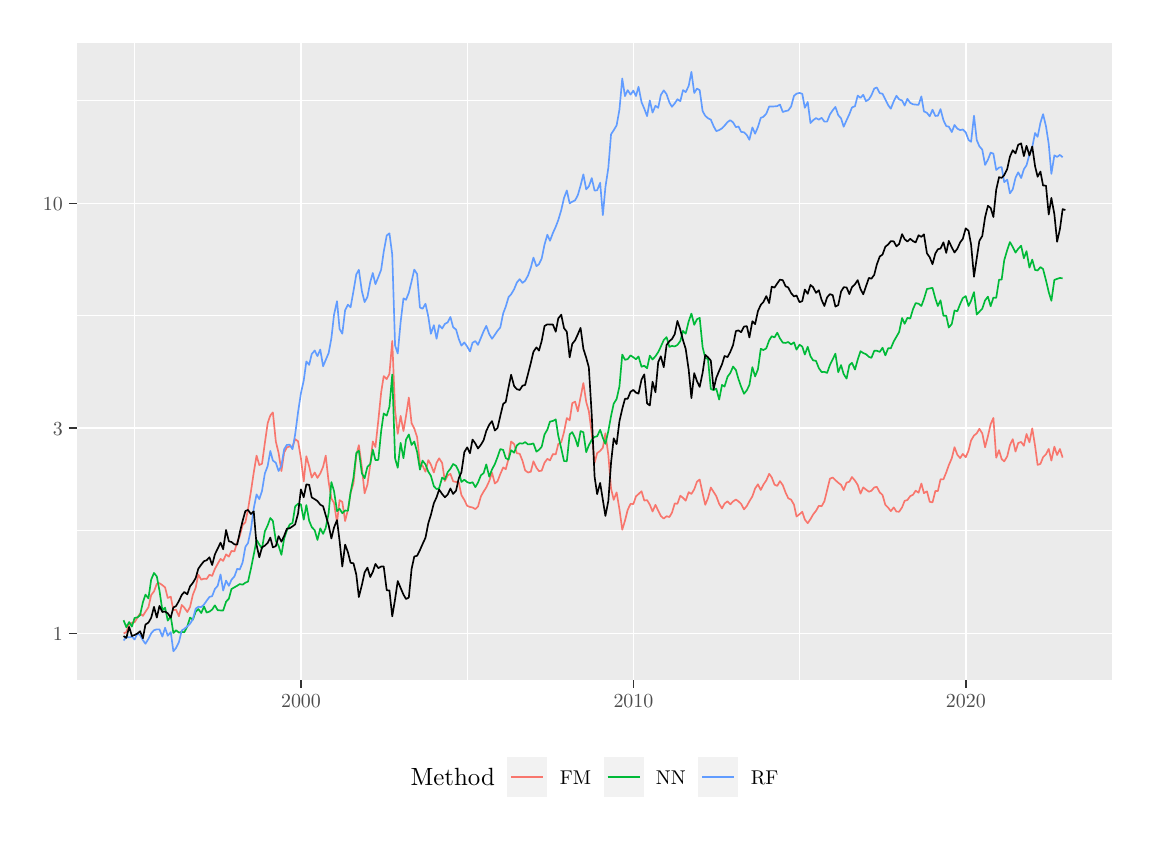
\begin{tikzpicture}[x=1pt,y=1pt]
\definecolor{fillColor}{RGB}{255,255,255}
\path[use as bounding box,fill=fillColor,fill opacity=0.00] (0,0) rectangle (397.48,289.08);
\begin{scope}
\path[clip] (  0.00,  0.00) rectangle (397.48,289.08);
\definecolor{drawColor}{RGB}{255,255,255}
\definecolor{fillColor}{RGB}{255,255,255}

\path[draw=drawColor,line width= 0.6pt,line join=round,line cap=round,fill=fillColor] (  0.00,  0.00) rectangle (397.48,289.08);
\end{scope}
\begin{scope}
\path[clip] ( 17.65, 53.26) rectangle (391.98,283.58);
\definecolor{fillColor}{gray}{0.92}

\path[fill=fillColor] ( 17.65, 53.26) rectangle (391.98,283.58);
\definecolor{drawColor}{RGB}{255,255,255}

\path[draw=drawColor,line width= 0.3pt,line join=round] ( 17.65,107.26) --
	(391.98,107.26);

\path[draw=drawColor,line width= 0.3pt,line join=round] ( 17.65,184.97) --
	(391.98,184.97);

\path[draw=drawColor,line width= 0.3pt,line join=round] ( 17.65,262.68) --
	(391.98,262.68);

\path[draw=drawColor,line width= 0.3pt,line join=round] ( 38.69, 53.26) --
	( 38.69,283.58);

\path[draw=drawColor,line width= 0.3pt,line join=round] (158.83, 53.26) --
	(158.83,283.58);

\path[draw=drawColor,line width= 0.3pt,line join=round] (278.94, 53.26) --
	(278.94,283.58);

\path[draw=drawColor,line width= 0.6pt,line join=round] ( 17.65, 70.18) --
	(391.98, 70.18);

\path[draw=drawColor,line width= 0.6pt,line join=round] ( 17.65,144.33) --
	(391.98,144.33);

\path[draw=drawColor,line width= 0.6pt,line join=round] ( 17.65,225.60) --
	(391.98,225.60);

\path[draw=drawColor,line width= 0.6pt,line join=round] ( 98.76, 53.26) --
	( 98.76,283.58);

\path[draw=drawColor,line width= 0.6pt,line join=round] (218.89, 53.26) --
	(218.89,283.58);

\path[draw=drawColor,line width= 0.6pt,line join=round] (338.99, 53.26) --
	(338.99,283.58);
\definecolor{drawColor}{RGB}{248,118,109}

\path[draw=drawColor,line width= 0.6pt,line join=round] ( 34.66, 70.20) --
	( 35.65, 70.67) --
	( 36.67, 73.56) --
	( 37.66, 74.05) --
	( 38.64, 74.23) --
	( 39.70, 76.01) --
	( 40.62, 77.38) --
	( 41.64, 76.54) --
	( 42.56, 78.02) --
	( 43.64, 79.62) --
	( 44.63, 84.06) --
	( 45.65, 85.38) --
	( 46.67, 88.13) --
	( 47.62, 88.35) --
	( 48.67, 87.64) --
	( 49.66, 86.81) --
	( 50.61, 83.00) --
	( 51.70, 83.46) --
	( 52.65, 78.63) --
	( 53.61, 78.74) --
	( 54.66, 76.40) --
	( 55.68, 80.48) --
	( 56.60, 79.51) --
	( 57.68, 77.92) --
	( 58.67, 79.72) --
	( 59.69, 84.18) --
	( 60.71, 86.72) --
	( 61.66, 91.44) --
	( 62.72, 89.60) --
	( 63.73, 90.00) --
	( 64.66, 89.87) --
	( 65.68, 91.38) --
	( 66.66, 90.97) --
	( 67.65, 93.49) --
	( 68.67, 95.36) --
	( 69.69, 97.13) --
	( 70.64, 96.39) --
	( 71.69, 98.75) --
	( 72.71, 97.95) --
	( 73.63, 99.99) --
	( 74.72, 99.84) --
	( 75.71,103.12) --
	( 76.63,105.34) --
	( 77.68,109.40) --
	( 78.67,110.35) --
	( 79.62,115.02) --
	( 80.67,121.48) --
	( 81.69,128.34) --
	( 82.71,134.44) --
	( 83.70,131.05) --
	( 84.68,131.51) --
	( 85.70,138.97) --
	( 86.72,146.10) --
	( 87.68,148.97) --
	( 88.60,150.05) --
	( 89.68,139.48) --
	( 90.67,135.42) --
	( 91.69,128.86) --
	( 92.67,135.54) --
	( 93.66,137.41) --
	( 94.71,137.78) --
	( 95.70,137.66) --
	( 96.65,140.38) --
	( 97.71,139.61) --
	( 98.73,133.53) --
	( 99.75,125.13) --
	(100.70,134.20) --
	(101.72,130.55) --
	(102.64,126.50) --
	(103.72,128.33) --
	(104.71,126.38) --
	(105.73,128.00) --
	(106.75,130.40) --
	(107.70,134.44) --
	(108.76,124.91) --
	(109.74,118.98) --
	(110.70,117.34) --
	(111.78,110.25) --
	(112.70,118.34) --
	(113.69,117.70) --
	(114.71,110.81) --
	(115.73,114.90) --
	(116.68,121.00) --
	(117.73,124.42) --
	(118.75,134.49) --
	(119.67,138.24) --
	(120.76,130.22) --
	(121.75,120.82) --
	(122.77,123.95) --
	(123.79,131.22) --
	(124.71,139.58) --
	(125.66,137.55) --
	(126.71,147.21) --
	(127.73,157.29) --
	(128.65,163.17) --
	(129.74,162.09) --
	(130.72,163.98) --
	(131.74,175.89) --
	(132.76,150.82) --
	(133.72,142.30) --
	(134.77,148.80) --
	(135.79,143.33) --
	(136.71,148.71) --
	(137.73,155.44) --
	(138.72,146.16) --
	(139.70,144.25) --
	(140.72,141.16) --
	(141.74,131.62) --
	(142.69,130.80) --
	(143.75,128.63) --
	(144.77,132.82) --
	(145.69,131.21) --
	(146.77,128.34) --
	(147.76,131.84) --
	(148.68,133.48) --
	(149.77,131.78) --
	(150.75,125.25) --
	(151.77,127.26) --
	(152.76,127.84) --
	(153.74,125.15) --
	(154.80,124.93) --
	(155.78,124.77) --
	(156.74,120.14) --
	(157.79,118.42) --
	(158.81,116.30) --
	(159.83,115.88) --
	(160.75,115.70) --
	(161.77,115.12) --
	(162.72,116.03) --
	(163.77,119.71) --
	(164.76,121.45) --
	(165.71,122.94) --
	(166.80,125.27) --
	(167.79,128.25) --
	(168.81,124.36) --
	(169.79,125.17) --
	(170.78,127.77) --
	(171.83,130.18) --
	(172.75,129.52) --
	(173.77,133.36) --
	(174.69,139.55) --
	(175.78,138.59) --
	(176.76,135.30) --
	(177.78,135.13) --
	(178.80,132.57) --
	(179.76,129.12) --
	(180.81,128.33) --
	(181.80,128.62) --
	(182.75,132.40) --
	(183.84,130.05) --
	(184.76,128.84) --
	(185.74,129.01) --
	(186.76,131.88) --
	(187.78,133.27) --
	(188.74,132.71) --
	(189.79,135.00) --
	(190.81,134.88) --
	(191.73,138.63) --
	(192.81,139.29) --
	(193.80,142.92) --
	(194.82,148.02) --
	(195.84,147.20) --
	(196.79,153.40) --
	(197.81,153.95) --
	(198.80,150.41) --
	(199.79,155.55) --
	(200.80,160.67) --
	(201.82,153.85) --
	(202.78,150.48) --
	(203.83,142.43) --
	(204.85,131.83) --
	(205.77,135.33) --
	(206.86,136.15) --
	(207.84,137.30) --
	(208.76,142.51) --
	(209.82,134.67) --
	(210.80,122.56) --
	(211.76,118.47) --
	(212.81,121.17) --
	(213.83,115.09) --
	(214.85,107.68) --
	(215.83,110.91) --
	(216.82,114.85) --
	(217.84,117.02) --
	(218.86,116.95) --
	(219.81,119.73) --
	(220.73,120.55) --
	(221.82,121.57) --
	(222.81,118.20) --
	(223.82,118.37) --
	(224.81,116.71) --
	(225.80,114.25) --
	(226.85,116.65) --
	(227.84,114.53) --
	(228.79,112.63) --
	(229.84,111.68) --
	(230.86,112.54) --
	(231.88,112.25) --
	(232.80,113.79) --
	(233.82,117.15) --
	(234.78,117.04) --
	(235.83,119.96) --
	(236.81,119.17) --
	(237.77,118.15) --
	(238.85,121.23) --
	(239.84,120.60) --
	(240.86,122.27) --
	(241.85,125.04) --
	(242.83,125.80) --
	(243.89,120.84) --
	(244.84,116.68) --
	(245.83,119.07) --
	(246.85,122.92) --
	(247.86,121.32) --
	(248.82,119.81) --
	(249.87,117.01) --
	(250.89,115.35) --
	(251.81,117.09) --
	(252.90,117.94) --
	(253.88,116.83) --
	(254.90,117.89) --
	(255.92,118.58) --
	(256.84,117.91) --
	(257.80,117.03) --
	(258.85,115.01) --
	(259.87,116.26) --
	(260.79,117.94) --
	(261.87,119.72) --
	(262.86,122.56) --
	(263.88,124.07) --
	(264.90,122.04) --
	(265.85,123.96) --
	(266.91,125.51) --
	(267.93,127.87) --
	(268.85,126.60) --
	(269.87,123.96) --
	(270.85,123.49) --
	(271.84,125.22) --
	(272.86,123.76) --
	(273.88,121.05) --
	(274.83,119.06) --
	(275.88,118.50) --
	(276.90,116.71) --
	(277.82,112.44) --
	(278.91,113.27) --
	(279.90,114.14) --
	(280.82,111.33) --
	(281.87,110.03) --
	(282.86,111.48) --
	(283.81,113.16) --
	(284.86,114.48) --
	(285.88,116.31) --
	(286.90,116.16) --
	(287.89,117.94) --
	(288.87,121.93) --
	(289.89,126.11) --
	(290.91,126.53) --
	(291.87,125.57) --
	(292.89,124.65) --
	(293.91,123.88) --
	(294.86,121.99) --
	(295.91,124.69) --
	(296.90,124.99) --
	(297.85,126.70) --
	(298.94,125.40) --
	(299.92,123.89) --
	(300.94,120.69) --
	(301.93,122.96) --
	(302.92,122.17) --
	(303.97,121.39) --
	(304.89,121.75) --
	(305.91,122.94) --
	(306.83,123.16) --
	(307.91,121.13) --
	(308.90,120.22) --
	(309.92,116.62) --
	(310.94,115.63) --
	(311.89,114.38) --
	(312.95,115.73) --
	(313.93,114.21) --
	(314.89,114.17) --
	(315.97,115.78) --
	(316.89,118.10) --
	(317.88,118.39) --
	(318.90,119.79) --
	(319.92,120.31) --
	(320.87,121.77) --
	(321.92,121.03) --
	(322.94,124.35) --
	(323.86,120.87) --
	(324.95,121.55) --
	(325.94,117.78) --
	(326.96,117.53) --
	(327.98,121.64) --
	(328.90,121.64) --
	(329.85,125.88) --
	(330.90,125.86) --
	(331.92,128.37) --
	(332.84,130.97) --
	(333.93,133.50) --
	(334.91,137.50) --
	(335.93,134.74) --
	(336.95,133.56) --
	(337.91,135.04) --
	(338.96,133.85) --
	(339.98,136.25) --
	(340.90,139.93) --
	(341.95,141.70) --
	(342.94,142.49) --
	(343.89,144.12) --
	(344.94,142.48) --
	(345.96,137.46) --
	(346.98,141.44) --
	(347.97,145.82) --
	(348.96,148.05) --
	(349.98,133.67) --
	(351.00,136.41) --
	(351.95,133.18) --
	(352.87,132.35) --
	(353.96,134.19) --
	(354.94,138.27) --
	(355.96,140.37) --
	(356.95,135.90) --
	(357.93,138.99) --
	(358.99,139.38) --
	(359.97,137.99) --
	(360.93,142.26) --
	(361.98,139.23) --
	(363.00,144.29) --
	(364.02,137.96) --
	(364.94,131.08) --
	(365.96,131.46) --
	(366.91,133.87) --
	(367.96,134.91) --
	(368.95,136.86) --
	(369.91,132.63) --
	(370.99,137.67) --
	(371.98,134.66) --
	(373.00,136.83) --
	(373.98,133.73);
\definecolor{drawColor}{RGB}{0,186,56}

\path[draw=drawColor,line width= 0.6pt,line join=round] ( 34.66, 74.95) --
	( 35.65, 72.44) --
	( 36.67, 74.31) --
	( 37.66, 72.67) --
	( 38.64, 75.80) --
	( 39.70, 75.99) --
	( 40.62, 76.80) --
	( 41.64, 81.48) --
	( 42.56, 84.22) --
	( 43.64, 82.86) --
	( 44.63, 89.66) --
	( 45.65, 92.04) --
	( 46.67, 90.76) --
	( 47.62, 85.67) --
	( 48.67, 78.58) --
	( 49.66, 79.52) --
	( 50.61, 74.82) --
	( 51.70, 76.34) --
	( 52.65, 70.35) --
	( 53.61, 71.32) --
	( 54.66, 70.51) --
	( 55.68, 70.73) --
	( 56.60, 70.62) --
	( 57.68, 72.71) --
	( 58.67, 75.91) --
	( 59.69, 75.15) --
	( 60.71, 78.02) --
	( 61.66, 79.00) --
	( 62.72, 77.57) --
	( 63.73, 79.93) --
	( 64.66, 77.73) --
	( 65.68, 78.06) --
	( 66.66, 78.81) --
	( 67.65, 80.33) --
	( 68.67, 78.58) --
	( 69.69, 78.50) --
	( 70.64, 78.45) --
	( 71.69, 81.67) --
	( 72.71, 82.75) --
	( 73.63, 86.21) --
	( 74.72, 86.86) --
	( 75.71, 87.42) --
	( 76.63, 88.03) --
	( 77.68, 87.81) --
	( 78.67, 88.53) --
	( 79.62, 88.90) --
	( 80.67, 93.59) --
	( 81.69, 98.62) --
	( 82.71,104.00) --
	( 83.70,102.33) --
	( 84.68,100.86) --
	( 85.70,107.05) --
	( 86.72,109.24) --
	( 87.68,111.90) --
	( 88.60,110.88) --
	( 89.68,103.68) --
	( 90.67,101.85) --
	( 91.69, 98.58) --
	( 92.67,104.46) --
	( 93.66,107.42) --
	( 94.71,109.59) --
	( 95.70,110.09) --
	( 96.65,116.06) --
	( 97.71,117.09) --
	( 98.73,116.83) --
	( 99.75,111.31) --
	(100.70,116.58) --
	(101.72,110.89) --
	(102.64,108.63) --
	(103.72,107.48) --
	(104.71,103.97) --
	(105.73,108.16) --
	(106.75,106.17) --
	(107.70,108.34) --
	(108.76,113.67) --
	(109.74,124.88) --
	(110.70,121.62) --
	(111.78,114.38) --
	(112.70,115.25) --
	(113.69,113.63) --
	(114.71,114.60) --
	(115.73,114.52) --
	(116.68,121.11) --
	(117.73,126.52) --
	(118.75,135.37) --
	(119.67,136.25) --
	(120.76,128.03) --
	(121.75,126.28) --
	(122.77,130.41) --
	(123.79,131.44) --
	(124.71,136.60) --
	(125.66,132.82) --
	(126.71,132.90) --
	(127.73,143.29) --
	(128.65,149.67) --
	(129.74,148.88) --
	(130.72,152.06) --
	(131.74,163.73) --
	(132.76,133.45) --
	(133.72,130.04) --
	(134.77,139.03) --
	(135.79,133.52) --
	(136.71,140.19) --
	(137.73,142.08) --
	(138.72,138.29) --
	(139.70,139.53) --
	(140.72,135.76) --
	(141.74,129.38) --
	(142.69,132.62) --
	(143.75,131.24) --
	(144.77,128.60) --
	(145.69,127.18) --
	(146.77,123.39) --
	(147.76,122.35) --
	(148.68,122.64) --
	(149.77,126.52) --
	(150.75,125.79) --
	(151.77,128.46) --
	(152.76,129.71) --
	(153.74,131.40) --
	(154.80,130.75) --
	(155.78,128.71) --
	(156.74,124.92) --
	(157.79,125.75) --
	(158.81,124.87) --
	(159.83,124.51) --
	(160.75,124.83) --
	(161.77,123.05) --
	(162.72,124.68) --
	(163.77,127.32) --
	(164.76,128.12) --
	(165.71,131.26) --
	(166.80,126.81) --
	(167.79,129.48) --
	(168.81,131.37) --
	(169.79,133.94) --
	(170.78,136.81) --
	(171.83,136.48) --
	(172.75,133.52) --
	(173.77,132.99) --
	(174.69,136.39) --
	(175.78,135.49) --
	(176.76,138.12) --
	(177.78,138.91) --
	(178.80,138.76) --
	(179.76,139.32) --
	(180.81,138.49) --
	(181.80,138.58) --
	(182.75,138.85) --
	(183.84,135.87) --
	(184.76,136.53) --
	(185.74,137.63) --
	(186.76,142.08) --
	(187.78,143.83) --
	(188.74,146.74) --
	(189.79,146.97) --
	(190.81,147.52) --
	(191.73,141.64) --
	(192.81,137.02) --
	(193.80,132.48) --
	(194.82,132.41) --
	(195.84,142.11) --
	(196.79,142.92) --
	(197.81,140.77) --
	(198.80,137.75) --
	(199.79,143.31) --
	(200.80,142.89) --
	(201.82,135.67) --
	(202.78,138.18) --
	(203.83,140.15) --
	(204.85,141.20) --
	(205.77,141.42) --
	(206.86,143.76) --
	(207.84,140.85) --
	(208.76,138.69) --
	(209.82,143.33) --
	(210.80,148.74) --
	(211.76,153.21) --
	(212.81,154.89) --
	(213.83,159.44) --
	(214.85,170.94) --
	(215.83,169.07) --
	(216.82,169.31) --
	(217.84,170.66) --
	(218.86,169.98) --
	(219.81,169.25) --
	(220.73,170.25) --
	(221.82,166.56) --
	(222.81,166.92) --
	(223.82,165.98) --
	(224.81,170.57) --
	(225.80,169.18) --
	(226.85,170.35) --
	(227.84,171.84) --
	(228.79,173.82) --
	(229.84,176.19) --
	(230.86,177.27) --
	(231.88,173.73) --
	(232.80,174.08) --
	(233.82,173.89) --
	(234.78,174.43) --
	(235.83,175.85) --
	(236.81,179.49) --
	(237.77,178.48) --
	(238.85,182.95) --
	(239.84,185.76) --
	(240.86,181.71) --
	(241.85,183.71) --
	(242.83,184.22) --
	(243.89,173.59) --
	(244.84,169.84) --
	(245.83,169.27) --
	(246.85,158.52) --
	(247.86,158.10) --
	(248.82,158.65) --
	(249.87,154.69) --
	(250.89,159.97) --
	(251.81,159.39) --
	(252.90,162.96) --
	(253.88,164.27) --
	(254.90,166.62) --
	(255.92,165.35) --
	(256.84,162.10) --
	(257.80,159.35) --
	(258.85,156.79) --
	(259.87,158.07) --
	(260.79,159.96) --
	(261.87,166.40) --
	(262.86,163.05) --
	(263.88,165.63) --
	(264.90,173.04) --
	(265.85,172.59) --
	(266.91,173.22) --
	(267.93,176.09) --
	(268.85,177.57) --
	(269.87,177.16) --
	(270.85,178.85) --
	(271.84,176.80) --
	(272.86,175.26) --
	(273.88,175.16) --
	(274.83,175.49) --
	(275.88,174.62) --
	(276.90,175.38) --
	(277.82,172.73) --
	(278.91,174.52) --
	(279.90,173.83) --
	(280.82,170.96) --
	(281.87,173.76) --
	(282.86,170.35) --
	(283.81,168.87) --
	(284.86,168.68) --
	(285.88,166.06) --
	(286.90,164.64) --
	(287.89,164.71) --
	(288.87,164.32) --
	(289.89,167.18) --
	(290.91,169.25) --
	(291.87,171.29) --
	(292.89,164.56) --
	(293.91,167.16) --
	(294.86,163.89) --
	(295.91,162.28) --
	(296.90,167.10) --
	(297.85,167.99) --
	(298.94,165.53) --
	(299.92,169.07) --
	(300.94,172.16) --
	(301.93,171.51) --
	(302.92,171.10) --
	(303.97,170.13) --
	(304.89,169.78) --
	(305.91,172.32) --
	(306.83,172.34) --
	(307.91,171.91) --
	(308.90,173.42) --
	(309.92,170.65) --
	(310.94,173.26) --
	(311.89,173.19) --
	(312.95,175.72) --
	(313.93,177.41) --
	(314.89,179.09) --
	(315.97,184.16) --
	(316.89,182.06) --
	(317.88,184.21) --
	(318.90,183.96) --
	(319.92,187.39) --
	(320.87,189.54) --
	(321.92,189.34) --
	(322.94,188.52) --
	(323.86,191.02) --
	(324.95,194.65) --
	(325.94,194.86) --
	(326.96,195.05) --
	(327.98,191.21) --
	(328.90,188.50) --
	(329.85,190.57) --
	(330.90,184.99) --
	(331.92,184.99) --
	(332.84,180.72) --
	(333.93,182.01) --
	(334.91,186.88) --
	(335.93,186.62) --
	(336.95,189.23) --
	(337.91,191.37) --
	(338.96,192.06) --
	(339.98,188.49) --
	(340.90,190.42) --
	(341.95,193.52) --
	(342.94,185.42) --
	(343.89,186.43) --
	(344.94,187.55) --
	(345.96,190.55) --
	(346.98,191.88) --
	(347.97,188.44) --
	(348.96,191.54) --
	(349.98,191.46) --
	(351.00,197.99) --
	(351.95,198.06) --
	(352.87,205.03) --
	(353.96,208.74) --
	(354.94,211.61) --
	(355.96,209.84) --
	(356.95,207.79) --
	(357.93,209.19) --
	(358.99,210.28) --
	(359.97,205.74) --
	(360.93,208.33) --
	(361.98,202.38) --
	(363.00,205.26) --
	(364.02,201.54) --
	(364.94,201.34) --
	(365.96,202.56) --
	(366.91,201.85) --
	(367.96,197.78) --
	(368.95,193.56) --
	(369.91,190.40) --
	(370.99,197.93) --
	(371.98,198.30) --
	(373.00,198.63) --
	(373.98,198.52);
\definecolor{drawColor}{RGB}{97,156,255}

\path[draw=drawColor,line width= 0.6pt,line join=round] ( 34.66, 67.63) --
	( 35.65, 68.90) --
	( 36.67, 68.76) --
	( 37.66, 69.01) --
	( 38.64, 68.01) --
	( 39.70, 70.19) --
	( 40.62, 69.53) --
	( 41.64, 67.76) --
	( 42.56, 66.47) --
	( 43.64, 68.24) --
	( 44.63, 70.23) --
	( 45.65, 71.35) --
	( 46.67, 71.67) --
	( 47.62, 71.65) --
	( 48.67, 69.03) --
	( 49.66, 72.24) --
	( 50.61, 69.35) --
	( 51.70, 70.67) --
	( 52.65, 63.73) --
	( 53.61, 64.92) --
	( 54.66, 67.08) --
	( 55.68, 71.28) --
	( 56.60, 71.83) --
	( 57.68, 72.74) --
	( 58.67, 73.68) --
	( 59.69, 75.33) --
	( 60.71, 79.14) --
	( 61.66, 79.82) --
	( 62.72, 79.71) --
	( 63.73, 80.64) --
	( 64.66, 82.00) --
	( 65.68, 83.37) --
	( 66.66, 83.67) --
	( 67.65, 86.24) --
	( 68.67, 87.41) --
	( 69.69, 91.50) --
	( 70.64, 85.69) --
	( 71.69, 89.28) --
	( 72.71, 87.37) --
	( 73.63, 89.57) --
	( 74.72, 90.79) --
	( 75.71, 93.54) --
	( 76.63, 93.28) --
	( 77.68, 95.90) --
	( 78.67,101.48) --
	( 79.62,102.85) --
	( 80.67,107.71) --
	( 81.69,115.34) --
	( 82.71,120.43) --
	( 83.70,118.70) --
	( 84.68,121.71) --
	( 85.70,127.98) --
	( 86.72,130.65) --
	( 87.68,136.13) --
	( 88.60,132.67) --
	( 89.68,131.86) --
	( 90.67,128.88) --
	( 91.69,130.77) --
	( 92.67,136.73) --
	( 93.66,138.33) --
	( 94.71,138.35) --
	( 95.70,136.74) --
	( 96.65,142.10) --
	( 97.71,150.20) --
	( 98.73,156.93) --
	( 99.75,161.56) --
	(100.70,168.47) --
	(101.72,167.24) --
	(102.64,171.14) --
	(103.72,172.42) --
	(104.71,170.40) --
	(105.73,172.77) --
	(106.75,166.73) --
	(107.70,169.01) --
	(108.76,171.51) --
	(109.74,176.82) --
	(110.70,185.36) --
	(111.78,190.24) --
	(112.70,180.23) --
	(113.69,178.49) --
	(114.71,187.01) --
	(115.73,188.99) --
	(116.68,188.05) --
	(117.73,193.91) --
	(118.75,199.93) --
	(119.67,201.58) --
	(120.76,193.89) --
	(121.75,189.92) --
	(122.77,191.76) --
	(123.79,197.14) --
	(124.71,200.43) --
	(125.66,196.39) --
	(126.71,198.96) --
	(127.73,201.62) --
	(128.65,208.08) --
	(129.74,213.98) --
	(130.72,214.78) --
	(131.74,207.03) --
	(132.76,174.23) --
	(133.72,171.35) --
	(134.77,182.72) --
	(135.79,191.26) --
	(136.71,190.76) --
	(137.73,193.29) --
	(138.72,197.40) --
	(139.70,201.65) --
	(140.72,200.08) --
	(141.74,187.99) --
	(142.69,187.52) --
	(143.75,189.31) --
	(144.77,184.67) --
	(145.69,178.46) --
	(146.77,181.57) --
	(147.76,176.68) --
	(148.68,181.60) --
	(149.77,180.37) --
	(150.75,182.03) --
	(151.77,182.59) --
	(152.76,184.53) --
	(153.74,180.84) --
	(154.80,179.99) --
	(155.78,176.56) --
	(156.74,174.18) --
	(157.79,175.34) --
	(158.81,173.85) --
	(159.83,172.08) --
	(160.75,175.23) --
	(161.77,175.83) --
	(162.72,174.46) --
	(163.77,176.98) --
	(164.76,179.40) --
	(165.71,181.33) --
	(166.80,178.31) --
	(167.79,176.68) --
	(168.81,178.08) --
	(169.79,179.57) --
	(170.78,180.75) --
	(171.83,185.87) --
	(172.75,188.27) --
	(173.77,191.72) --
	(174.69,192.73) --
	(175.78,194.57) --
	(176.76,196.97) --
	(177.78,198.19) --
	(178.80,196.85) --
	(179.76,197.63) --
	(180.81,199.54) --
	(181.80,202.34) --
	(182.75,206.00) --
	(183.84,202.90) --
	(184.76,203.62) --
	(185.74,205.68) --
	(186.76,210.68) --
	(187.78,214.26) --
	(188.74,212.08) --
	(189.79,214.88) --
	(190.81,217.13) --
	(191.73,219.55) --
	(192.81,223.19) --
	(193.80,227.54) --
	(194.82,230.25) --
	(195.84,225.61) --
	(196.79,226.20) --
	(197.81,226.68) --
	(198.80,228.58) --
	(199.79,232.04) --
	(200.80,236.08) --
	(201.82,230.65) --
	(202.78,231.72) --
	(203.83,234.72) --
	(204.85,230.23) --
	(205.77,230.31) --
	(206.86,233.02) --
	(207.84,221.34) --
	(208.76,231.41) --
	(209.82,238.45) --
	(210.80,250.54) --
	(211.76,252.02) --
	(212.81,253.76) --
	(213.83,259.45) --
	(214.85,270.69) --
	(215.83,264.36) --
	(216.82,266.52) --
	(217.84,264.88) --
	(218.86,266.34) --
	(219.81,264.38) --
	(220.73,267.73) --
	(221.82,262.15) --
	(222.81,259.81) --
	(223.82,257.12) --
	(224.81,262.76) --
	(225.80,258.39) --
	(226.85,260.85) --
	(227.84,260.12) --
	(228.79,264.75) --
	(229.84,266.42) --
	(230.86,265.05) --
	(231.88,262.04) --
	(232.80,260.49) --
	(233.82,261.72) --
	(234.78,263.22) --
	(235.83,262.52) --
	(236.81,266.52) --
	(237.77,265.79) --
	(238.85,268.01) --
	(239.84,273.11) --
	(240.86,265.47) --
	(241.85,267.07) --
	(242.83,266.49) --
	(243.89,258.93) --
	(244.84,257.22) --
	(245.83,256.34) --
	(246.85,255.85) --
	(247.86,253.47) --
	(248.82,251.69) --
	(249.87,252.08) --
	(250.89,252.70) --
	(251.81,253.67) --
	(252.90,254.97) --
	(253.88,255.65) --
	(254.90,254.84) --
	(255.92,253.12) --
	(256.84,253.37) --
	(257.80,251.43) --
	(258.85,251.27) --
	(259.87,250.23) --
	(260.79,248.60) --
	(261.87,253.03) --
	(262.86,250.77) --
	(263.88,253.18) --
	(264.90,256.49) --
	(265.85,256.87) --
	(266.91,258.00) --
	(267.93,260.59) --
	(268.85,260.57) --
	(269.87,260.64) --
	(270.85,260.73) --
	(271.84,261.30) --
	(272.86,258.60) --
	(273.88,258.94) --
	(274.83,259.16) --
	(275.88,260.61) --
	(276.90,264.44) --
	(277.82,265.22) --
	(278.91,265.50) --
	(279.90,265.18) --
	(280.82,260.13) --
	(281.87,262.24) --
	(282.86,254.61) --
	(283.81,255.63) --
	(284.86,256.39) --
	(285.88,255.85) --
	(286.90,256.50) --
	(287.89,255.14) --
	(288.87,255.14) --
	(289.89,257.73) --
	(290.91,259.25) --
	(291.87,260.44) --
	(292.89,257.50) --
	(293.91,256.29) --
	(294.86,253.28) --
	(295.91,255.65) --
	(296.90,257.79) --
	(297.85,260.25) --
	(298.94,260.69) --
	(299.92,264.53) --
	(300.94,263.72) --
	(301.93,264.82) --
	(302.92,262.50) --
	(303.97,263.17) --
	(304.89,264.67) --
	(305.91,267.08) --
	(306.83,267.46) --
	(307.91,265.40) --
	(308.90,265.21) --
	(309.92,263.10) --
	(310.94,261.06) --
	(311.89,259.80) --
	(312.95,262.49) --
	(313.93,264.47) --
	(314.89,263.17) --
	(315.97,262.77) --
	(316.89,260.92) --
	(317.88,263.37) --
	(318.90,261.91) --
	(319.92,261.39) --
	(320.87,261.28) --
	(321.92,261.18) --
	(322.94,264.23) --
	(323.86,258.81) --
	(324.95,258.30) --
	(325.94,257.05) --
	(326.96,259.43) --
	(327.98,257.17) --
	(328.90,257.26) --
	(329.85,259.66) --
	(330.90,255.66) --
	(331.92,253.50) --
	(332.84,253.31) --
	(333.93,251.35) --
	(334.91,253.91) --
	(335.93,252.59) --
	(336.95,252.05) --
	(337.91,252.29) --
	(338.96,251.26) --
	(339.98,248.51) --
	(340.90,247.84) --
	(341.95,257.27) --
	(342.94,248.47) --
	(343.89,246.23) --
	(344.94,244.99) --
	(345.96,239.48) --
	(346.98,241.36) --
	(347.97,243.93) --
	(348.96,243.54) --
	(349.98,237.65) --
	(351.00,238.54) --
	(351.95,238.67) --
	(352.87,233.25) --
	(353.96,234.19) --
	(354.94,229.20) --
	(355.96,230.69) --
	(356.95,234.81) --
	(357.93,236.81) --
	(358.99,234.73) --
	(359.97,237.90) --
	(360.93,239.36) --
	(361.98,243.25) --
	(363.00,245.87) --
	(364.02,251.03) --
	(364.94,249.61) --
	(365.96,254.72) --
	(366.91,257.82) --
	(367.96,253.48) --
	(368.95,247.08) --
	(369.91,236.24) --
	(370.99,242.93) --
	(371.98,242.37) --
	(373.00,243.10) --
	(373.98,242.27);
\definecolor{drawColor}{RGB}{0,0,0}

\path[draw=drawColor,line width= 0.6pt,line join=round] ( 34.66, 69.24) --
	( 35.65, 68.55) --
	( 36.67, 72.55) --
	( 37.66, 69.26) --
	( 38.64, 69.61) --
	( 39.70, 70.18) --
	( 40.62, 70.98) --
	( 41.64, 68.45) --
	( 42.56, 73.40) --
	( 43.64, 74.10) --
	( 44.63, 75.84) --
	( 45.65, 79.78) --
	( 46.67, 75.91) --
	( 47.62, 80.14) --
	( 48.67, 77.93) --
	( 49.66, 78.11) --
	( 50.61, 77.48) --
	( 51.70, 75.90) --
	( 52.65, 79.58) --
	( 53.61, 80.08) --
	( 54.66, 81.92) --
	( 55.68, 84.11) --
	( 56.60, 85.16) --
	( 57.68, 84.33) --
	( 58.67, 87.20) --
	( 59.69, 88.47) --
	( 60.71, 90.20) --
	( 61.66, 93.57) --
	( 62.72, 95.05) --
	( 63.73, 96.32) --
	( 64.66, 96.63) --
	( 65.68, 97.72) --
	( 66.66, 94.90) --
	( 67.65, 98.75) --
	( 68.67,100.84) --
	( 69.69,103.01) --
	( 70.64,100.61) --
	( 71.69,107.56) --
	( 72.71,103.45) --
	( 73.63,103.23) --
	( 74.72,102.37) --
	( 75.71,102.28) --
	( 76.63,106.58) --
	( 77.68,110.92) --
	( 78.67,114.44) --
	( 79.62,114.80) --
	( 80.67,113.34) --
	( 81.69,114.29) --
	( 82.71,102.14) --
	( 83.70, 97.71) --
	( 84.68,101.31) --
	( 85.70,101.90) --
	( 86.72,102.89) --
	( 87.68,104.83) --
	( 88.60,101.26) --
	( 89.68,101.76) --
	( 90.67,105.35) --
	( 91.69,103.34) --
	( 92.67,105.42) --
	( 93.66,108.00) --
	( 94.71,108.22) --
	( 95.70,108.88) --
	( 96.65,109.59) --
	( 97.71,113.53) --
	( 98.73,122.24) --
	( 99.75,119.38) --
	(100.70,124.04) --
	(101.72,123.87) --
	(102.64,119.34) --
	(103.72,118.69) --
	(104.71,118.03) --
	(105.73,116.72) --
	(106.75,116.15) --
	(107.70,112.86) --
	(108.76,109.27) --
	(109.74,104.49) --
	(110.70,108.48) --
	(111.78,111.14) --
	(112.70,103.67) --
	(113.69, 94.38) --
	(114.71,102.29) --
	(115.73, 99.51) --
	(116.68, 95.70) --
	(117.73, 95.54) --
	(118.75, 91.43) --
	(119.67, 83.34) --
	(120.76, 87.66) --
	(121.75, 92.23) --
	(122.77, 93.96) --
	(123.79, 90.58) --
	(124.71, 92.39) --
	(125.66, 95.32) --
	(126.71, 93.77) --
	(127.73, 94.37) --
	(128.65, 94.41) --
	(129.74, 85.80) --
	(130.72, 85.70) --
	(131.74, 76.36) --
	(132.76, 82.56) --
	(133.72, 89.12) --
	(134.77, 86.61) --
	(135.79, 84.22) --
	(136.71, 82.64) --
	(137.73, 83.16) --
	(138.72, 93.44) --
	(139.70, 97.97) --
	(140.72, 98.26) --
	(141.74,100.29) --
	(142.69,102.48) --
	(143.75,104.76) --
	(144.77,110.00) --
	(145.69,112.98) --
	(146.77,117.25) --
	(147.76,119.38) --
	(148.68,122.15) --
	(149.77,120.57) --
	(150.75,119.40) --
	(151.77,120.36) --
	(152.76,122.57) --
	(153.74,120.59) --
	(154.80,121.80) --
	(155.78,126.29) --
	(156.74,128.45) --
	(157.79,135.72) --
	(158.81,137.42) --
	(159.83,135.30) --
	(160.75,140.24) --
	(161.77,138.82) --
	(162.72,137.02) --
	(163.77,138.36) --
	(164.76,140.03) --
	(165.71,143.34) --
	(166.80,145.64) --
	(167.79,146.91) --
	(168.81,143.52) --
	(169.79,144.44) --
	(170.78,148.79) --
	(171.83,153.14) --
	(172.75,153.82) --
	(173.77,159.17) --
	(174.69,163.66) --
	(175.78,159.55) --
	(176.76,158.45) --
	(177.78,158.13) --
	(178.80,159.69) --
	(179.76,159.98) --
	(180.81,164.01) --
	(181.80,167.90) --
	(182.75,171.96) --
	(183.84,173.56) --
	(184.76,172.38) --
	(185.74,175.89) --
	(186.76,181.26) --
	(187.78,181.88) --
	(188.74,181.81) --
	(189.79,181.80) --
	(190.81,179.21) --
	(191.73,184.03) --
	(192.81,185.35) --
	(193.80,180.50) --
	(194.82,179.20) --
	(195.84,169.95) --
	(196.79,174.86) --
	(197.81,176.10) --
	(198.80,178.28) --
	(199.79,180.59) --
	(200.80,173.03) --
	(201.82,169.85) --
	(202.78,166.29) --
	(203.83,148.98) --
	(204.85,126.88) --
	(205.77,120.51) --
	(206.86,124.59) --
	(207.84,118.43) --
	(208.76,112.65) --
	(209.82,118.06) --
	(210.80,131.88) --
	(211.76,140.70) --
	(212.81,138.58) --
	(213.83,146.85) --
	(214.85,151.32) --
	(215.83,154.96) --
	(216.82,155.01) --
	(217.84,157.51) --
	(218.86,158.18) --
	(219.81,157.21) --
	(220.73,156.84) --
	(221.82,161.95) --
	(222.81,163.79) --
	(223.82,153.31) --
	(224.81,152.56) --
	(225.80,161.12) --
	(226.85,157.34) --
	(227.84,168.22) --
	(228.79,170.32) --
	(229.84,166.40) --
	(230.86,174.40) --
	(231.88,175.80) --
	(232.80,176.56) --
	(233.82,178.32) --
	(234.78,183.10) --
	(235.83,179.89) --
	(236.81,176.12) --
	(237.77,173.02) --
	(238.85,165.52) --
	(239.84,155.23) --
	(240.86,164.23) --
	(241.85,161.36) --
	(242.83,159.27) --
	(243.89,164.39) --
	(244.84,170.83) --
	(245.83,169.96) --
	(246.85,168.78) --
	(247.86,158.42) --
	(248.82,162.51) --
	(249.87,165.09) --
	(250.89,167.44) --
	(251.81,170.43) --
	(252.90,170.05) --
	(253.88,171.91) --
	(254.90,174.42) --
	(255.92,179.44) --
	(256.84,179.69) --
	(257.80,179.04) --
	(258.85,181.07) --
	(259.87,181.22) --
	(260.79,177.14) --
	(261.87,183.01) --
	(262.86,181.94) --
	(263.88,186.67) --
	(264.90,188.92) --
	(265.85,189.94) --
	(266.91,192.08) --
	(267.93,189.55) --
	(268.85,195.48) --
	(269.87,195.16) --
	(270.85,196.66) --
	(271.84,198.02) --
	(272.86,197.83) --
	(273.88,195.62) --
	(274.83,195.21) --
	(275.88,193.14) --
	(276.90,191.96) --
	(277.82,192.30) --
	(278.91,189.87) --
	(279.90,190.28) --
	(280.82,194.45) --
	(281.87,192.90) --
	(282.86,196.10) --
	(283.81,195.30) --
	(284.86,193.27) --
	(285.88,194.19) --
	(286.90,190.65) --
	(287.89,188.51) --
	(288.87,191.62) --
	(289.89,192.80) --
	(290.91,192.40) --
	(291.87,188.32) --
	(292.89,188.80) --
	(293.91,193.71) --
	(294.86,195.26) --
	(295.91,195.24) --
	(296.90,192.80) --
	(297.85,195.31) --
	(298.94,196.35) --
	(299.92,197.85) --
	(300.94,194.63) --
	(301.93,192.74) --
	(302.92,195.60) --
	(303.97,198.66) --
	(304.89,198.37) --
	(305.91,199.79) --
	(306.83,203.50) --
	(307.91,206.40) --
	(308.90,207.10) --
	(309.92,209.94) --
	(310.94,210.74) --
	(311.89,211.94) --
	(312.95,211.86) --
	(313.93,210.07) --
	(314.89,210.89) --
	(315.97,214.48) --
	(316.89,212.66) --
	(317.88,211.78) --
	(318.90,212.80) --
	(319.92,211.95) --
	(320.87,211.47) --
	(321.92,214.07) --
	(322.94,213.48) --
	(323.86,214.39) --
	(324.95,207.54) --
	(325.94,206.12) --
	(326.96,203.60) --
	(327.98,207.46) --
	(328.90,209.01) --
	(329.85,209.26) --
	(330.90,211.51) --
	(331.92,207.70) --
	(332.84,212.03) --
	(333.93,209.68) --
	(334.91,207.84) --
	(335.93,209.19) --
	(336.95,211.49) --
	(337.91,212.77) --
	(338.96,216.58) --
	(339.98,215.68) --
	(340.90,210.69) --
	(341.95,199.08) --
	(342.94,205.74) --
	(343.89,212.05) --
	(344.94,213.81) --
	(345.96,220.57) --
	(346.98,224.72) --
	(347.97,223.94) --
	(348.96,220.67) --
	(349.98,230.54) --
	(351.00,235.05) --
	(351.95,234.81) --
	(352.87,235.79) --
	(353.96,238.04) --
	(354.94,242.51) --
	(355.96,244.79) --
	(356.95,243.65) --
	(357.93,246.77) --
	(358.99,247.24) --
	(359.97,242.65) --
	(360.93,246.38) --
	(361.98,242.91) --
	(363.00,246.14) --
	(364.02,239.01) --
	(364.94,235.21) --
	(365.96,237.08) --
	(366.91,232.04) --
	(367.96,232.00) --
	(368.95,221.56) --
	(369.91,227.54) --
	(370.99,221.70) --
	(371.98,211.73) --
	(373.00,216.28) --
	(373.98,223.50) --
	(374.97,223.18);
\end{scope}
\begin{scope}
\path[clip] (  0.00,  0.00) rectangle (397.48,289.08);
\definecolor{drawColor}{gray}{0.30}

\node[text=drawColor,anchor=base east,inner sep=0pt, outer sep=0pt, scale=  0.72] at ( 12.70, 67.70) {1};

\node[text=drawColor,anchor=base east,inner sep=0pt, outer sep=0pt, scale=  0.72] at ( 12.70,141.86) {3};

\node[text=drawColor,anchor=base east,inner sep=0pt, outer sep=0pt, scale=  0.72] at ( 12.70,223.12) {10};
\end{scope}
\begin{scope}
\path[clip] (  0.00,  0.00) rectangle (397.48,289.08);
\definecolor{drawColor}{gray}{0.20}

\path[draw=drawColor,line width= 0.6pt,line join=round] ( 14.90, 70.18) --
	( 17.65, 70.18);

\path[draw=drawColor,line width= 0.6pt,line join=round] ( 14.90,144.33) --
	( 17.65,144.33);

\path[draw=drawColor,line width= 0.6pt,line join=round] ( 14.90,225.60) --
	( 17.65,225.60);
\end{scope}
\begin{scope}
\path[clip] (  0.00,  0.00) rectangle (397.48,289.08);
\definecolor{drawColor}{gray}{0.20}

\path[draw=drawColor,line width= 0.6pt,line join=round] ( 98.76, 50.51) --
	( 98.76, 53.26);

\path[draw=drawColor,line width= 0.6pt,line join=round] (218.89, 50.51) --
	(218.89, 53.26);

\path[draw=drawColor,line width= 0.6pt,line join=round] (338.99, 50.51) --
	(338.99, 53.26);
\end{scope}
\begin{scope}
\path[clip] (  0.00,  0.00) rectangle (397.48,289.08);
\definecolor{drawColor}{gray}{0.30}

\node[text=drawColor,anchor=base,inner sep=0pt, outer sep=0pt, scale=  0.72] at ( 98.76, 43.35) {2000};

\node[text=drawColor,anchor=base,inner sep=0pt, outer sep=0pt, scale=  0.72] at (218.89, 43.35) {2010};

\node[text=drawColor,anchor=base,inner sep=0pt, outer sep=0pt, scale=  0.72] at (338.99, 43.35) {2020};
\end{scope}
\begin{scope}
\path[clip] (  0.00,  0.00) rectangle (397.48,289.08);
\definecolor{fillColor}{RGB}{255,255,255}

\path[fill=fillColor] (132.84,  5.50) rectangle (276.79, 30.95);
\end{scope}
\begin{scope}
\path[clip] (  0.00,  0.00) rectangle (397.48,289.08);
\definecolor{drawColor}{RGB}{0,0,0}

\node[text=drawColor,anchor=base west,inner sep=0pt, outer sep=0pt, scale=  0.90] at (138.34, 15.13) {Method};
\end{scope}
\begin{scope}
\path[clip] (  0.00,  0.00) rectangle (397.48,289.08);
\definecolor{fillColor}{gray}{0.95}

\path[fill=fillColor] (173.34, 11.00) rectangle (187.79, 25.45);
\end{scope}
\begin{scope}
\path[clip] (  0.00,  0.00) rectangle (397.48,289.08);
\definecolor{drawColor}{RGB}{248,118,109}

\path[draw=drawColor,line width= 0.6pt,line join=round] (174.78, 18.23) -- (186.34, 18.23);
\end{scope}
\begin{scope}
\path[clip] (  0.00,  0.00) rectangle (397.48,289.08);
\definecolor{fillColor}{gray}{0.95}

\path[fill=fillColor] (208.09, 11.00) rectangle (222.54, 25.45);
\end{scope}
\begin{scope}
\path[clip] (  0.00,  0.00) rectangle (397.48,289.08);
\definecolor{drawColor}{RGB}{0,186,56}

\path[draw=drawColor,line width= 0.6pt,line join=round] (209.53, 18.23) -- (221.10, 18.23);
\end{scope}
\begin{scope}
\path[clip] (  0.00,  0.00) rectangle (397.48,289.08);
\definecolor{fillColor}{gray}{0.95}

\path[fill=fillColor] (242.34, 11.00) rectangle (256.79, 25.45);
\end{scope}
\begin{scope}
\path[clip] (  0.00,  0.00) rectangle (397.48,289.08);
\definecolor{drawColor}{RGB}{97,156,255}

\path[draw=drawColor,line width= 0.6pt,line join=round] (243.78, 18.23) -- (255.35, 18.23);
\end{scope}
\begin{scope}
\path[clip] (  0.00,  0.00) rectangle (397.48,289.08);
\definecolor{drawColor}{RGB}{0,0,0}

\node[text=drawColor,anchor=base west,inner sep=0pt, outer sep=0pt, scale=  0.72] at (192.29, 15.75) {FM};
\end{scope}
\begin{scope}
\path[clip] (  0.00,  0.00) rectangle (397.48,289.08);
\definecolor{drawColor}{RGB}{0,0,0}

\node[text=drawColor,anchor=base west,inner sep=0pt, outer sep=0pt, scale=  0.72] at (227.04, 15.75) {NN};
\end{scope}
\begin{scope}
\path[clip] (  0.00,  0.00) rectangle (397.48,289.08);
\definecolor{drawColor}{RGB}{0,0,0}

\node[text=drawColor,anchor=base west,inner sep=0pt, outer sep=0pt, scale=  0.72] at (261.29, 15.75) {RF};
\end{scope}
\end{tikzpicture}

\label{plot:cumul_vw_LS_portf_return}
\end{figure}

\begin{figure}[h]
\centering
\caption[Relative variable importance]{\textbf{..}\\ ...}
% Created by tikzDevice version 0.12.6 on 2024-03-21 19:32:39
% !TEX encoding = UTF-8 Unicode
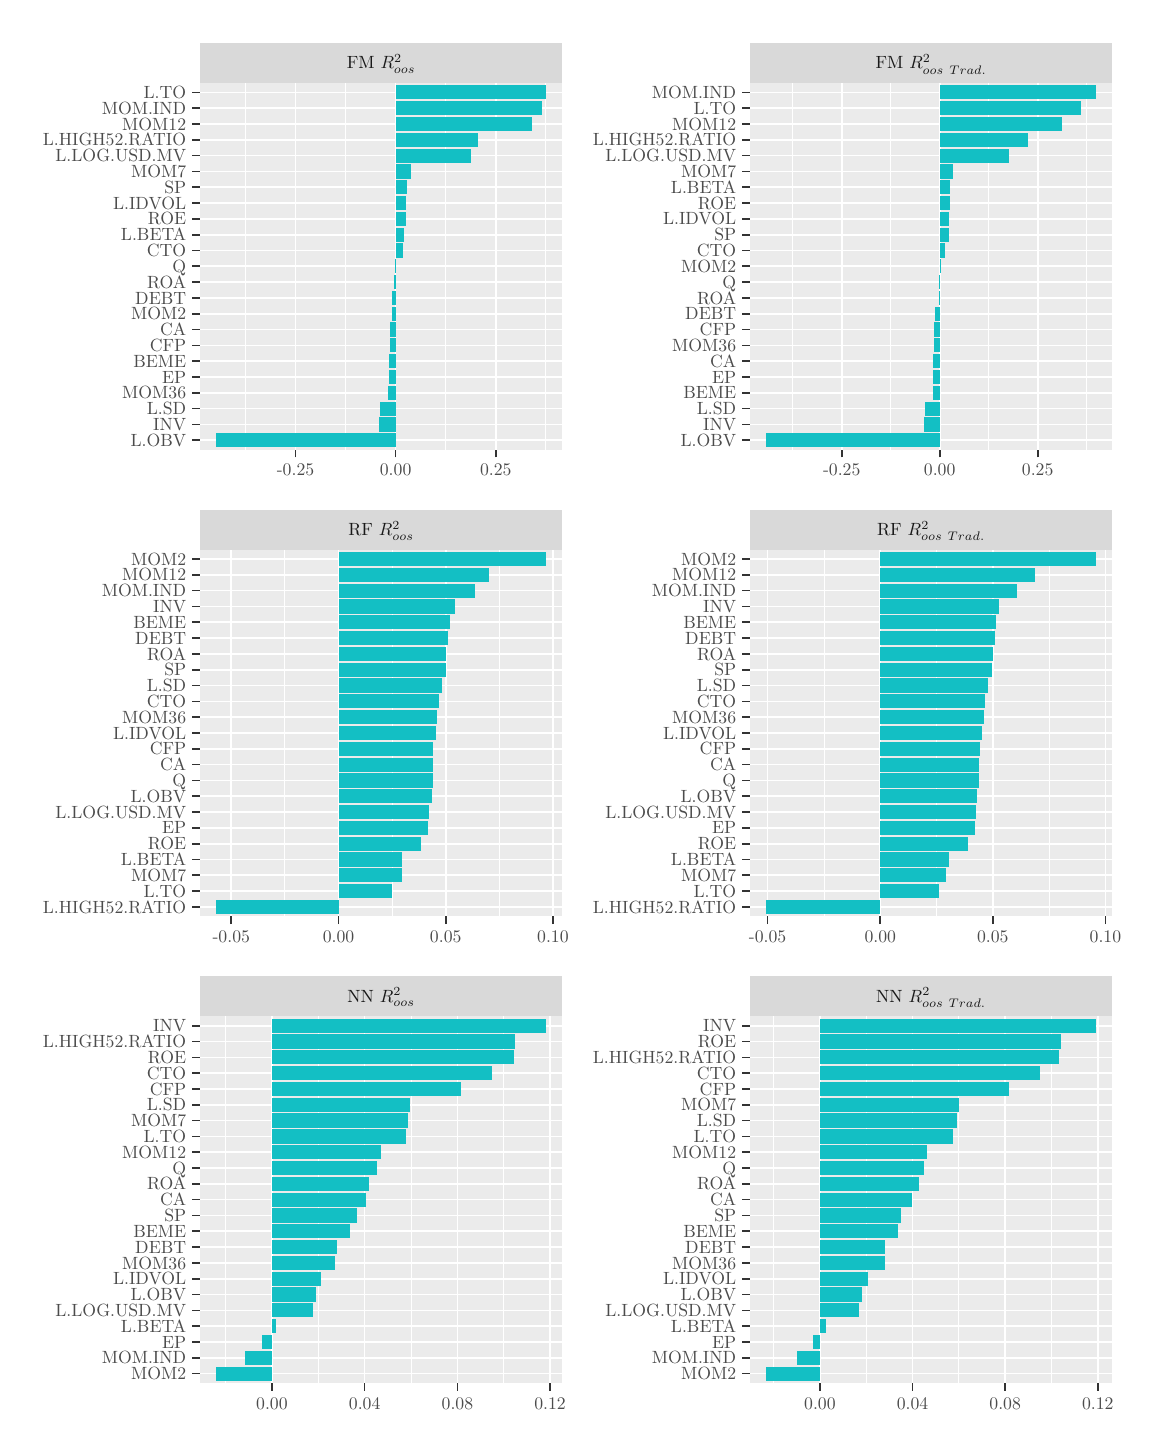
\begin{tikzpicture}[x=1pt,y=1pt]
\definecolor{fillColor}{RGB}{255,255,255}
\path[use as bounding box,fill=fillColor,fill opacity=0.00] (0,0) rectangle (397.48,505.89);
\begin{scope}
\path[clip] (  0.00,337.26) rectangle (198.74,505.89);
\definecolor{drawColor}{RGB}{255,255,255}
\definecolor{fillColor}{RGB}{255,255,255}

\path[draw=drawColor,line width= 0.6pt,line join=round,line cap=round,fill=fillColor] (  0.00,337.26) rectangle (198.74,505.89);
\end{scope}
\begin{scope}
\path[clip] ( 62.22,353.36) rectangle (193.24,485.94);
\definecolor{fillColor}{gray}{0.92}

\path[fill=fillColor] ( 62.22,353.36) rectangle (193.24,485.94);
\definecolor{drawColor}{RGB}{255,255,255}

\path[draw=drawColor,line width= 0.3pt,line join=round] ( 78.70,353.36) --
	( 78.70,485.94);

\path[draw=drawColor,line width= 0.3pt,line join=round] (114.88,353.36) --
	(114.88,485.94);

\path[draw=drawColor,line width= 0.3pt,line join=round] (151.05,353.36) --
	(151.05,485.94);

\path[draw=drawColor,line width= 0.3pt,line join=round] (187.23,353.36) --
	(187.23,485.94);

\path[draw=drawColor,line width= 0.6pt,line join=round] ( 62.22,356.79) --
	(193.24,356.79);

\path[draw=drawColor,line width= 0.6pt,line join=round] ( 62.22,362.51) --
	(193.24,362.51);

\path[draw=drawColor,line width= 0.6pt,line join=round] ( 62.22,368.22) --
	(193.24,368.22);

\path[draw=drawColor,line width= 0.6pt,line join=round] ( 62.22,373.93) --
	(193.24,373.93);

\path[draw=drawColor,line width= 0.6pt,line join=round] ( 62.22,379.65) --
	(193.24,379.65);

\path[draw=drawColor,line width= 0.6pt,line join=round] ( 62.22,385.36) --
	(193.24,385.36);

\path[draw=drawColor,line width= 0.6pt,line join=round] ( 62.22,391.08) --
	(193.24,391.08);

\path[draw=drawColor,line width= 0.6pt,line join=round] ( 62.22,396.79) --
	(193.24,396.79);

\path[draw=drawColor,line width= 0.6pt,line join=round] ( 62.22,402.51) --
	(193.24,402.51);

\path[draw=drawColor,line width= 0.6pt,line join=round] ( 62.22,408.22) --
	(193.24,408.22);

\path[draw=drawColor,line width= 0.6pt,line join=round] ( 62.22,413.94) --
	(193.24,413.94);

\path[draw=drawColor,line width= 0.6pt,line join=round] ( 62.22,419.65) --
	(193.24,419.65);

\path[draw=drawColor,line width= 0.6pt,line join=round] ( 62.22,425.36) --
	(193.24,425.36);

\path[draw=drawColor,line width= 0.6pt,line join=round] ( 62.22,431.08) --
	(193.24,431.08);

\path[draw=drawColor,line width= 0.6pt,line join=round] ( 62.22,436.79) --
	(193.24,436.79);

\path[draw=drawColor,line width= 0.6pt,line join=round] ( 62.22,442.51) --
	(193.24,442.51);

\path[draw=drawColor,line width= 0.6pt,line join=round] ( 62.22,448.22) --
	(193.24,448.22);

\path[draw=drawColor,line width= 0.6pt,line join=round] ( 62.22,453.94) --
	(193.24,453.94);

\path[draw=drawColor,line width= 0.6pt,line join=round] ( 62.22,459.65) --
	(193.24,459.65);

\path[draw=drawColor,line width= 0.6pt,line join=round] ( 62.22,465.37) --
	(193.24,465.37);

\path[draw=drawColor,line width= 0.6pt,line join=round] ( 62.22,471.08) --
	(193.24,471.08);

\path[draw=drawColor,line width= 0.6pt,line join=round] ( 62.22,476.79) --
	(193.24,476.79);

\path[draw=drawColor,line width= 0.6pt,line join=round] ( 62.22,482.51) --
	(193.24,482.51);

\path[draw=drawColor,line width= 0.6pt,line join=round] ( 96.79,353.36) --
	( 96.79,485.94);

\path[draw=drawColor,line width= 0.6pt,line join=round] (132.96,353.36) --
	(132.96,485.94);

\path[draw=drawColor,line width= 0.6pt,line join=round] (169.14,353.36) --
	(169.14,485.94);
\definecolor{fillColor}{RGB}{19,191,196}

\path[fill=fillColor] (130.99,394.22) rectangle (132.96,399.36);

\path[fill=fillColor] (132.96,422.79) rectangle (135.58,427.94);

\path[fill=fillColor] (130.56,382.79) rectangle (132.96,387.93);

\path[fill=fillColor] (130.92,388.51) rectangle (132.96,393.65);

\path[fill=fillColor] (126.96,359.93) rectangle (132.96,365.08);

\path[fill=fillColor] (131.76,405.65) rectangle (132.96,410.79);

\path[fill=fillColor] (132.96,445.65) rectangle (136.90,450.79);

\path[fill=fillColor] (130.49,377.08) rectangle (132.96,382.22);

\path[fill=fillColor] (132.55,411.36) rectangle (132.96,416.51);

\path[fill=fillColor] (132.96,434.22) rectangle (136.57,439.36);

\path[fill=fillColor] (132.90,417.08) rectangle (132.96,422.22);

\path[fill=fillColor] (132.96,451.37) rectangle (138.34,456.51);

\path[fill=fillColor] (132.96,468.51) rectangle (182.41,473.65);

\path[fill=fillColor] (130.38,371.36) rectangle (132.96,376.51);

\path[fill=fillColor] (131.63,399.94) rectangle (132.96,405.08);

\path[fill=fillColor] (132.96,474.22) rectangle (185.98,479.37);

\path[fill=fillColor] (127.27,365.65) rectangle (132.96,370.79);

\path[fill=fillColor] (132.96,462.79) rectangle (162.64,467.94);

\path[fill=fillColor] (132.96,428.51) rectangle (135.89,433.65);

\path[fill=fillColor] (132.96,439.94) rectangle (136.60,445.08);

\path[fill=fillColor] (132.96,457.08) rectangle (160.11,462.22);

\path[fill=fillColor] (132.96,479.94) rectangle (187.29,485.08);

\path[fill=fillColor] ( 68.17,354.22) rectangle (132.96,359.36);
\end{scope}
\begin{scope}
\path[clip] ( 62.22,485.94) rectangle (193.24,500.39);
\definecolor{fillColor}{gray}{0.85}

\path[fill=fillColor] ( 62.22,485.94) rectangle (193.24,500.39);
\definecolor{drawColor}{gray}{0.10}

\node[text=drawColor,anchor=base,inner sep=0pt, outer sep=0pt, scale=  0.64] at (127.73,490.96) {FM $R^2_{oos}$};
\end{scope}
\begin{scope}
\path[clip] (  0.00,  0.00) rectangle (397.48,505.89);
\definecolor{drawColor}{gray}{0.20}

\path[draw=drawColor,line width= 0.6pt,line join=round] ( 96.79,350.61) --
	( 96.79,353.36);

\path[draw=drawColor,line width= 0.6pt,line join=round] (132.96,350.61) --
	(132.96,353.36);

\path[draw=drawColor,line width= 0.6pt,line join=round] (169.14,350.61) --
	(169.14,353.36);
\end{scope}
\begin{scope}
\path[clip] (  0.00,  0.00) rectangle (397.48,505.89);
\definecolor{drawColor}{gray}{0.30}

\node[text=drawColor,anchor=base,inner sep=0pt, outer sep=0pt, scale=  0.64] at ( 96.79,344.00) {-0.25};

\node[text=drawColor,anchor=base,inner sep=0pt, outer sep=0pt, scale=  0.64] at (132.96,344.00) {0.00};

\node[text=drawColor,anchor=base,inner sep=0pt, outer sep=0pt, scale=  0.64] at (169.14,344.00) {0.25};
\end{scope}
\begin{scope}
\path[clip] (  0.00,  0.00) rectangle (397.48,505.89);
\definecolor{drawColor}{gray}{0.30}

\node[text=drawColor,anchor=base east,inner sep=0pt, outer sep=0pt, scale=  0.64] at ( 57.27,354.59) {L.OBV};

\node[text=drawColor,anchor=base east,inner sep=0pt, outer sep=0pt, scale=  0.64] at ( 57.27,360.30) {INV};

\node[text=drawColor,anchor=base east,inner sep=0pt, outer sep=0pt, scale=  0.64] at ( 57.27,366.02) {L.SD};

\node[text=drawColor,anchor=base east,inner sep=0pt, outer sep=0pt, scale=  0.64] at ( 57.27,371.73) {MOM36};

\node[text=drawColor,anchor=base east,inner sep=0pt, outer sep=0pt, scale=  0.64] at ( 57.27,377.44) {EP};

\node[text=drawColor,anchor=base east,inner sep=0pt, outer sep=0pt, scale=  0.64] at ( 57.27,383.16) {BEME};

\node[text=drawColor,anchor=base east,inner sep=0pt, outer sep=0pt, scale=  0.64] at ( 57.27,388.87) {CFP};

\node[text=drawColor,anchor=base east,inner sep=0pt, outer sep=0pt, scale=  0.64] at ( 57.27,394.59) {CA};

\node[text=drawColor,anchor=base east,inner sep=0pt, outer sep=0pt, scale=  0.64] at ( 57.27,400.30) {MOM2};

\node[text=drawColor,anchor=base east,inner sep=0pt, outer sep=0pt, scale=  0.64] at ( 57.27,406.02) {DEBT};

\node[text=drawColor,anchor=base east,inner sep=0pt, outer sep=0pt, scale=  0.64] at ( 57.27,411.73) {ROA};

\node[text=drawColor,anchor=base east,inner sep=0pt, outer sep=0pt, scale=  0.64] at ( 57.27,417.45) {Q};

\node[text=drawColor,anchor=base east,inner sep=0pt, outer sep=0pt, scale=  0.64] at ( 57.27,423.16) {CTO};

\node[text=drawColor,anchor=base east,inner sep=0pt, outer sep=0pt, scale=  0.64] at ( 57.27,428.88) {L.BETA};

\node[text=drawColor,anchor=base east,inner sep=0pt, outer sep=0pt, scale=  0.64] at ( 57.27,434.59) {ROE};

\node[text=drawColor,anchor=base east,inner sep=0pt, outer sep=0pt, scale=  0.64] at ( 57.27,440.30) {L.IDVOL};

\node[text=drawColor,anchor=base east,inner sep=0pt, outer sep=0pt, scale=  0.64] at ( 57.27,446.02) {SP};

\node[text=drawColor,anchor=base east,inner sep=0pt, outer sep=0pt, scale=  0.64] at ( 57.27,451.73) {MOM7};

\node[text=drawColor,anchor=base east,inner sep=0pt, outer sep=0pt, scale=  0.64] at ( 57.27,457.45) {L.LOG.USD.MV};

\node[text=drawColor,anchor=base east,inner sep=0pt, outer sep=0pt, scale=  0.64] at ( 57.27,463.16) {L.HIGH52.RATIO};

\node[text=drawColor,anchor=base east,inner sep=0pt, outer sep=0pt, scale=  0.64] at ( 57.27,468.88) {MOM12};

\node[text=drawColor,anchor=base east,inner sep=0pt, outer sep=0pt, scale=  0.64] at ( 57.27,474.59) {MOM.IND};

\node[text=drawColor,anchor=base east,inner sep=0pt, outer sep=0pt, scale=  0.64] at ( 57.27,480.31) {L.TO};
\end{scope}
\begin{scope}
\path[clip] (  0.00,  0.00) rectangle (397.48,505.89);
\definecolor{drawColor}{gray}{0.20}

\path[draw=drawColor,line width= 0.6pt,line join=round] ( 59.47,356.79) --
	( 62.22,356.79);

\path[draw=drawColor,line width= 0.6pt,line join=round] ( 59.47,362.51) --
	( 62.22,362.51);

\path[draw=drawColor,line width= 0.6pt,line join=round] ( 59.47,368.22) --
	( 62.22,368.22);

\path[draw=drawColor,line width= 0.6pt,line join=round] ( 59.47,373.93) --
	( 62.22,373.93);

\path[draw=drawColor,line width= 0.6pt,line join=round] ( 59.47,379.65) --
	( 62.22,379.65);

\path[draw=drawColor,line width= 0.6pt,line join=round] ( 59.47,385.36) --
	( 62.22,385.36);

\path[draw=drawColor,line width= 0.6pt,line join=round] ( 59.47,391.08) --
	( 62.22,391.08);

\path[draw=drawColor,line width= 0.6pt,line join=round] ( 59.47,396.79) --
	( 62.22,396.79);

\path[draw=drawColor,line width= 0.6pt,line join=round] ( 59.47,402.51) --
	( 62.22,402.51);

\path[draw=drawColor,line width= 0.6pt,line join=round] ( 59.47,408.22) --
	( 62.22,408.22);

\path[draw=drawColor,line width= 0.6pt,line join=round] ( 59.47,413.94) --
	( 62.22,413.94);

\path[draw=drawColor,line width= 0.6pt,line join=round] ( 59.47,419.65) --
	( 62.22,419.65);

\path[draw=drawColor,line width= 0.6pt,line join=round] ( 59.47,425.36) --
	( 62.22,425.36);

\path[draw=drawColor,line width= 0.6pt,line join=round] ( 59.47,431.08) --
	( 62.22,431.08);

\path[draw=drawColor,line width= 0.6pt,line join=round] ( 59.47,436.79) --
	( 62.22,436.79);

\path[draw=drawColor,line width= 0.6pt,line join=round] ( 59.47,442.51) --
	( 62.22,442.51);

\path[draw=drawColor,line width= 0.6pt,line join=round] ( 59.47,448.22) --
	( 62.22,448.22);

\path[draw=drawColor,line width= 0.6pt,line join=round] ( 59.47,453.94) --
	( 62.22,453.94);

\path[draw=drawColor,line width= 0.6pt,line join=round] ( 59.47,459.65) --
	( 62.22,459.65);

\path[draw=drawColor,line width= 0.6pt,line join=round] ( 59.47,465.37) --
	( 62.22,465.37);

\path[draw=drawColor,line width= 0.6pt,line join=round] ( 59.47,471.08) --
	( 62.22,471.08);

\path[draw=drawColor,line width= 0.6pt,line join=round] ( 59.47,476.79) --
	( 62.22,476.79);

\path[draw=drawColor,line width= 0.6pt,line join=round] ( 59.47,482.51) --
	( 62.22,482.51);
\end{scope}
\begin{scope}
\path[clip] (198.74,337.26) rectangle (397.48,505.89);
\definecolor{drawColor}{RGB}{255,255,255}
\definecolor{fillColor}{RGB}{255,255,255}

\path[draw=drawColor,line width= 0.6pt,line join=round,line cap=round,fill=fillColor] (198.74,337.26) rectangle (397.48,505.89);
\end{scope}
\begin{scope}
\path[clip] (260.96,353.36) rectangle (391.98,485.94);
\definecolor{fillColor}{gray}{0.92}

\path[fill=fillColor] (260.96,353.36) rectangle (391.98,485.94);
\definecolor{drawColor}{RGB}{255,255,255}

\path[draw=drawColor,line width= 0.3pt,line join=round] (276.46,353.36) --
	(276.46,485.94);

\path[draw=drawColor,line width= 0.3pt,line join=round] (311.86,353.36) --
	(311.86,485.94);

\path[draw=drawColor,line width= 0.3pt,line join=round] (347.26,353.36) --
	(347.26,485.94);

\path[draw=drawColor,line width= 0.3pt,line join=round] (382.66,353.36) --
	(382.66,485.94);

\path[draw=drawColor,line width= 0.6pt,line join=round] (260.96,356.79) --
	(391.98,356.79);

\path[draw=drawColor,line width= 0.6pt,line join=round] (260.96,362.51) --
	(391.98,362.51);

\path[draw=drawColor,line width= 0.6pt,line join=round] (260.96,368.22) --
	(391.98,368.22);

\path[draw=drawColor,line width= 0.6pt,line join=round] (260.96,373.93) --
	(391.98,373.93);

\path[draw=drawColor,line width= 0.6pt,line join=round] (260.96,379.65) --
	(391.98,379.65);

\path[draw=drawColor,line width= 0.6pt,line join=round] (260.96,385.36) --
	(391.98,385.36);

\path[draw=drawColor,line width= 0.6pt,line join=round] (260.96,391.08) --
	(391.98,391.08);

\path[draw=drawColor,line width= 0.6pt,line join=round] (260.96,396.79) --
	(391.98,396.79);

\path[draw=drawColor,line width= 0.6pt,line join=round] (260.96,402.51) --
	(391.98,402.51);

\path[draw=drawColor,line width= 0.6pt,line join=round] (260.96,408.22) --
	(391.98,408.22);

\path[draw=drawColor,line width= 0.6pt,line join=round] (260.96,413.94) --
	(391.98,413.94);

\path[draw=drawColor,line width= 0.6pt,line join=round] (260.96,419.65) --
	(391.98,419.65);

\path[draw=drawColor,line width= 0.6pt,line join=round] (260.96,425.36) --
	(391.98,425.36);

\path[draw=drawColor,line width= 0.6pt,line join=round] (260.96,431.08) --
	(391.98,431.08);

\path[draw=drawColor,line width= 0.6pt,line join=round] (260.96,436.79) --
	(391.98,436.79);

\path[draw=drawColor,line width= 0.6pt,line join=round] (260.96,442.51) --
	(391.98,442.51);

\path[draw=drawColor,line width= 0.6pt,line join=round] (260.96,448.22) --
	(391.98,448.22);

\path[draw=drawColor,line width= 0.6pt,line join=round] (260.96,453.94) --
	(391.98,453.94);

\path[draw=drawColor,line width= 0.6pt,line join=round] (260.96,459.65) --
	(391.98,459.65);

\path[draw=drawColor,line width= 0.6pt,line join=round] (260.96,465.37) --
	(391.98,465.37);

\path[draw=drawColor,line width= 0.6pt,line join=round] (260.96,471.08) --
	(391.98,471.08);

\path[draw=drawColor,line width= 0.6pt,line join=round] (260.96,476.79) --
	(391.98,476.79);

\path[draw=drawColor,line width= 0.6pt,line join=round] (260.96,482.51) --
	(391.98,482.51);

\path[draw=drawColor,line width= 0.6pt,line join=round] (294.16,353.36) --
	(294.16,485.94);

\path[draw=drawColor,line width= 0.6pt,line join=round] (329.56,353.36) --
	(329.56,485.94);

\path[draw=drawColor,line width= 0.6pt,line join=round] (364.96,353.36) --
	(364.96,485.94);
\definecolor{fillColor}{RGB}{19,191,196}

\path[fill=fillColor] (327.28,382.79) rectangle (329.56,387.93);

\path[fill=fillColor] (329.56,422.79) rectangle (331.30,427.94);

\path[fill=fillColor] (326.97,371.36) rectangle (329.56,376.51);

\path[fill=fillColor] (327.50,394.22) rectangle (329.56,399.36);

\path[fill=fillColor] (323.82,359.93) rectangle (329.56,365.08);

\path[fill=fillColor] (328.01,399.94) rectangle (329.56,405.08);

\path[fill=fillColor] (329.56,428.51) rectangle (332.74,433.65);

\path[fill=fillColor] (327.02,377.08) rectangle (329.56,382.22);

\path[fill=fillColor] (329.26,405.65) rectangle (329.56,410.79);

\path[fill=fillColor] (329.56,439.94) rectangle (333.14,445.08);

\path[fill=fillColor] (329.45,411.36) rectangle (329.56,416.51);

\path[fill=fillColor] (329.56,451.37) rectangle (334.30,456.51);

\path[fill=fillColor] (329.56,468.51) rectangle (373.74,473.65);

\path[fill=fillColor] (327.45,388.51) rectangle (329.56,393.65);

\path[fill=fillColor] (329.56,417.08) rectangle (329.67,422.22);

\path[fill=fillColor] (329.56,479.94) rectangle (386.03,485.08);

\path[fill=fillColor] (324.37,365.65) rectangle (329.56,370.79);

\path[fill=fillColor] (329.56,462.79) rectangle (361.64,467.94);

\path[fill=fillColor] (329.56,445.65) rectangle (333.22,450.79);

\path[fill=fillColor] (329.56,434.22) rectangle (332.74,439.36);

\path[fill=fillColor] (329.56,457.08) rectangle (354.48,462.22);

\path[fill=fillColor] (329.56,474.22) rectangle (380.48,479.37);

\path[fill=fillColor] (266.91,354.22) rectangle (329.56,359.36);
\end{scope}
\begin{scope}
\path[clip] (260.96,485.94) rectangle (391.98,500.39);
\definecolor{fillColor}{gray}{0.85}

\path[fill=fillColor] (260.96,485.94) rectangle (391.98,500.39);
\definecolor{drawColor}{gray}{0.10}

\node[text=drawColor,anchor=base,inner sep=0pt, outer sep=0pt, scale=  0.64] at (326.47,490.96) {FM $R^2_{oos \ Trad.}$};
\end{scope}
\begin{scope}
\path[clip] (  0.00,  0.00) rectangle (397.48,505.89);
\definecolor{drawColor}{gray}{0.20}

\path[draw=drawColor,line width= 0.6pt,line join=round] (294.16,350.61) --
	(294.16,353.36);

\path[draw=drawColor,line width= 0.6pt,line join=round] (329.56,350.61) --
	(329.56,353.36);

\path[draw=drawColor,line width= 0.6pt,line join=round] (364.96,350.61) --
	(364.96,353.36);
\end{scope}
\begin{scope}
\path[clip] (  0.00,  0.00) rectangle (397.48,505.89);
\definecolor{drawColor}{gray}{0.30}

\node[text=drawColor,anchor=base,inner sep=0pt, outer sep=0pt, scale=  0.64] at (294.16,344.00) {-0.25};

\node[text=drawColor,anchor=base,inner sep=0pt, outer sep=0pt, scale=  0.64] at (329.56,344.00) {0.00};

\node[text=drawColor,anchor=base,inner sep=0pt, outer sep=0pt, scale=  0.64] at (364.96,344.00) {0.25};
\end{scope}
\begin{scope}
\path[clip] (  0.00,  0.00) rectangle (397.48,505.89);
\definecolor{drawColor}{gray}{0.30}

\node[text=drawColor,anchor=base east,inner sep=0pt, outer sep=0pt, scale=  0.64] at (256.01,354.59) {L.OBV};

\node[text=drawColor,anchor=base east,inner sep=0pt, outer sep=0pt, scale=  0.64] at (256.01,360.30) {INV};

\node[text=drawColor,anchor=base east,inner sep=0pt, outer sep=0pt, scale=  0.64] at (256.01,366.02) {L.SD};

\node[text=drawColor,anchor=base east,inner sep=0pt, outer sep=0pt, scale=  0.64] at (256.01,371.73) {BEME};

\node[text=drawColor,anchor=base east,inner sep=0pt, outer sep=0pt, scale=  0.64] at (256.01,377.44) {EP};

\node[text=drawColor,anchor=base east,inner sep=0pt, outer sep=0pt, scale=  0.64] at (256.01,383.16) {CA};

\node[text=drawColor,anchor=base east,inner sep=0pt, outer sep=0pt, scale=  0.64] at (256.01,388.87) {MOM36};

\node[text=drawColor,anchor=base east,inner sep=0pt, outer sep=0pt, scale=  0.64] at (256.01,394.59) {CFP};

\node[text=drawColor,anchor=base east,inner sep=0pt, outer sep=0pt, scale=  0.64] at (256.01,400.30) {DEBT};

\node[text=drawColor,anchor=base east,inner sep=0pt, outer sep=0pt, scale=  0.64] at (256.01,406.02) {ROA};

\node[text=drawColor,anchor=base east,inner sep=0pt, outer sep=0pt, scale=  0.64] at (256.01,411.73) {Q};

\node[text=drawColor,anchor=base east,inner sep=0pt, outer sep=0pt, scale=  0.64] at (256.01,417.45) {MOM2};

\node[text=drawColor,anchor=base east,inner sep=0pt, outer sep=0pt, scale=  0.64] at (256.01,423.16) {CTO};

\node[text=drawColor,anchor=base east,inner sep=0pt, outer sep=0pt, scale=  0.64] at (256.01,428.88) {SP};

\node[text=drawColor,anchor=base east,inner sep=0pt, outer sep=0pt, scale=  0.64] at (256.01,434.59) {L.IDVOL};

\node[text=drawColor,anchor=base east,inner sep=0pt, outer sep=0pt, scale=  0.64] at (256.01,440.30) {ROE};

\node[text=drawColor,anchor=base east,inner sep=0pt, outer sep=0pt, scale=  0.64] at (256.01,446.02) {L.BETA};

\node[text=drawColor,anchor=base east,inner sep=0pt, outer sep=0pt, scale=  0.64] at (256.01,451.73) {MOM7};

\node[text=drawColor,anchor=base east,inner sep=0pt, outer sep=0pt, scale=  0.64] at (256.01,457.45) {L.LOG.USD.MV};

\node[text=drawColor,anchor=base east,inner sep=0pt, outer sep=0pt, scale=  0.64] at (256.01,463.16) {L.HIGH52.RATIO};

\node[text=drawColor,anchor=base east,inner sep=0pt, outer sep=0pt, scale=  0.64] at (256.01,468.88) {MOM12};

\node[text=drawColor,anchor=base east,inner sep=0pt, outer sep=0pt, scale=  0.64] at (256.01,474.59) {L.TO};

\node[text=drawColor,anchor=base east,inner sep=0pt, outer sep=0pt, scale=  0.64] at (256.01,480.31) {MOM.IND};
\end{scope}
\begin{scope}
\path[clip] (  0.00,  0.00) rectangle (397.48,505.89);
\definecolor{drawColor}{gray}{0.20}

\path[draw=drawColor,line width= 0.6pt,line join=round] (258.21,356.79) --
	(260.96,356.79);

\path[draw=drawColor,line width= 0.6pt,line join=round] (258.21,362.51) --
	(260.96,362.51);

\path[draw=drawColor,line width= 0.6pt,line join=round] (258.21,368.22) --
	(260.96,368.22);

\path[draw=drawColor,line width= 0.6pt,line join=round] (258.21,373.93) --
	(260.96,373.93);

\path[draw=drawColor,line width= 0.6pt,line join=round] (258.21,379.65) --
	(260.96,379.65);

\path[draw=drawColor,line width= 0.6pt,line join=round] (258.21,385.36) --
	(260.96,385.36);

\path[draw=drawColor,line width= 0.6pt,line join=round] (258.21,391.08) --
	(260.96,391.08);

\path[draw=drawColor,line width= 0.6pt,line join=round] (258.21,396.79) --
	(260.96,396.79);

\path[draw=drawColor,line width= 0.6pt,line join=round] (258.21,402.51) --
	(260.96,402.51);

\path[draw=drawColor,line width= 0.6pt,line join=round] (258.21,408.22) --
	(260.96,408.22);

\path[draw=drawColor,line width= 0.6pt,line join=round] (258.21,413.94) --
	(260.96,413.94);

\path[draw=drawColor,line width= 0.6pt,line join=round] (258.21,419.65) --
	(260.96,419.65);

\path[draw=drawColor,line width= 0.6pt,line join=round] (258.21,425.36) --
	(260.96,425.36);

\path[draw=drawColor,line width= 0.6pt,line join=round] (258.21,431.08) --
	(260.96,431.08);

\path[draw=drawColor,line width= 0.6pt,line join=round] (258.21,436.79) --
	(260.96,436.79);

\path[draw=drawColor,line width= 0.6pt,line join=round] (258.21,442.51) --
	(260.96,442.51);

\path[draw=drawColor,line width= 0.6pt,line join=round] (258.21,448.22) --
	(260.96,448.22);

\path[draw=drawColor,line width= 0.6pt,line join=round] (258.21,453.94) --
	(260.96,453.94);

\path[draw=drawColor,line width= 0.6pt,line join=round] (258.21,459.65) --
	(260.96,459.65);

\path[draw=drawColor,line width= 0.6pt,line join=round] (258.21,465.37) --
	(260.96,465.37);

\path[draw=drawColor,line width= 0.6pt,line join=round] (258.21,471.08) --
	(260.96,471.08);

\path[draw=drawColor,line width= 0.6pt,line join=round] (258.21,476.79) --
	(260.96,476.79);

\path[draw=drawColor,line width= 0.6pt,line join=round] (258.21,482.51) --
	(260.96,482.51);
\end{scope}
\begin{scope}
\path[clip] (  0.00,168.63) rectangle (198.74,337.26);
\definecolor{drawColor}{RGB}{255,255,255}
\definecolor{fillColor}{RGB}{255,255,255}

\path[draw=drawColor,line width= 0.6pt,line join=round,line cap=round,fill=fillColor] (  0.00,168.63) rectangle (198.74,337.26);
\end{scope}
\begin{scope}
\path[clip] ( 62.22,184.73) rectangle (193.24,317.31);
\definecolor{fillColor}{gray}{0.92}

\path[fill=fillColor] ( 62.22,184.73) rectangle (193.24,317.31);
\definecolor{drawColor}{RGB}{255,255,255}

\path[draw=drawColor,line width= 0.3pt,line join=round] ( 92.94,184.73) --
	( 92.94,317.31);

\path[draw=drawColor,line width= 0.3pt,line join=round] (131.69,184.73) --
	(131.69,317.31);

\path[draw=drawColor,line width= 0.3pt,line join=round] (170.43,184.73) --
	(170.43,317.31);

\path[draw=drawColor,line width= 0.6pt,line join=round] ( 62.22,188.16) --
	(193.24,188.16);

\path[draw=drawColor,line width= 0.6pt,line join=round] ( 62.22,193.88) --
	(193.24,193.88);

\path[draw=drawColor,line width= 0.6pt,line join=round] ( 62.22,199.59) --
	(193.24,199.59);

\path[draw=drawColor,line width= 0.6pt,line join=round] ( 62.22,205.30) --
	(193.24,205.30);

\path[draw=drawColor,line width= 0.6pt,line join=round] ( 62.22,211.02) --
	(193.24,211.02);

\path[draw=drawColor,line width= 0.6pt,line join=round] ( 62.22,216.73) --
	(193.24,216.73);

\path[draw=drawColor,line width= 0.6pt,line join=round] ( 62.22,222.45) --
	(193.24,222.45);

\path[draw=drawColor,line width= 0.6pt,line join=round] ( 62.22,228.16) --
	(193.24,228.16);

\path[draw=drawColor,line width= 0.6pt,line join=round] ( 62.22,233.88) --
	(193.24,233.88);

\path[draw=drawColor,line width= 0.6pt,line join=round] ( 62.22,239.59) --
	(193.24,239.59);

\path[draw=drawColor,line width= 0.6pt,line join=round] ( 62.22,245.31) --
	(193.24,245.31);

\path[draw=drawColor,line width= 0.6pt,line join=round] ( 62.22,251.02) --
	(193.24,251.02);

\path[draw=drawColor,line width= 0.6pt,line join=round] ( 62.22,256.73) --
	(193.24,256.73);

\path[draw=drawColor,line width= 0.6pt,line join=round] ( 62.22,262.45) --
	(193.24,262.45);

\path[draw=drawColor,line width= 0.6pt,line join=round] ( 62.22,268.16) --
	(193.24,268.16);

\path[draw=drawColor,line width= 0.6pt,line join=round] ( 62.22,273.88) --
	(193.24,273.88);

\path[draw=drawColor,line width= 0.6pt,line join=round] ( 62.22,279.59) --
	(193.24,279.59);

\path[draw=drawColor,line width= 0.6pt,line join=round] ( 62.22,285.31) --
	(193.24,285.31);

\path[draw=drawColor,line width= 0.6pt,line join=round] ( 62.22,291.02) --
	(193.24,291.02);

\path[draw=drawColor,line width= 0.6pt,line join=round] ( 62.22,296.74) --
	(193.24,296.74);

\path[draw=drawColor,line width= 0.6pt,line join=round] ( 62.22,302.45) --
	(193.24,302.45);

\path[draw=drawColor,line width= 0.6pt,line join=round] ( 62.22,308.16) --
	(193.24,308.16);

\path[draw=drawColor,line width= 0.6pt,line join=round] ( 62.22,313.88) --
	(193.24,313.88);

\path[draw=drawColor,line width= 0.6pt,line join=round] ( 73.57,184.73) --
	( 73.57,317.31);

\path[draw=drawColor,line width= 0.6pt,line join=round] (112.32,184.73) --
	(112.32,317.31);

\path[draw=drawColor,line width= 0.6pt,line join=round] (151.06,184.73) --
	(151.06,317.31);

\path[draw=drawColor,line width= 0.6pt,line join=round] (189.80,184.73) --
	(189.80,317.31);
\definecolor{fillColor}{RGB}{19,191,196}

\path[fill=fillColor] (112.32,237.02) rectangle (146.46,242.16);

\path[fill=fillColor] (112.32,259.88) rectangle (148.61,265.02);

\path[fill=fillColor] (112.32,288.45) rectangle (152.56,293.59);

\path[fill=fillColor] (112.32,242.73) rectangle (146.60,247.88);

\path[fill=fillColor] (112.32,294.16) rectangle (154.34,299.31);

\path[fill=fillColor] (112.32,282.74) rectangle (151.74,287.88);

\path[fill=fillColor] (112.32,271.31) rectangle (150.98,276.45);

\path[fill=fillColor] (112.32,214.16) rectangle (144.56,219.30);

\path[fill=fillColor] (112.32,277.02) rectangle (151.26,282.16);

\path[fill=fillColor] (112.32,208.45) rectangle (142.07,213.59);

\path[fill=fillColor] (112.32,231.31) rectangle (146.43,236.45);

\path[fill=fillColor] (112.32,197.02) rectangle (135.23,202.16);

\path[fill=fillColor] (112.32,305.59) rectangle (166.77,310.74);

\path[fill=fillColor] (112.32,254.16) rectangle (147.96,259.31);

\path[fill=fillColor] (112.32,311.31) rectangle (187.29,316.45);

\path[fill=fillColor] (112.32,299.88) rectangle (161.81,305.02);

\path[fill=fillColor] (112.32,265.59) rectangle (149.65,270.73);

\path[fill=fillColor] ( 68.17,185.59) rectangle (112.32,190.73);

\path[fill=fillColor] (112.32,202.73) rectangle (135.32,207.88);

\path[fill=fillColor] (112.32,248.45) rectangle (147.66,253.59);

\path[fill=fillColor] (112.32,219.88) rectangle (144.90,225.02);

\path[fill=fillColor] (112.32,191.30) rectangle (131.70,196.45);

\path[fill=fillColor] (112.32,225.59) rectangle (145.98,230.73);
\end{scope}
\begin{scope}
\path[clip] ( 62.22,317.31) rectangle (193.24,331.76);
\definecolor{fillColor}{gray}{0.85}

\path[fill=fillColor] ( 62.22,317.31) rectangle (193.24,331.76);
\definecolor{drawColor}{gray}{0.10}

\node[text=drawColor,anchor=base,inner sep=0pt, outer sep=0pt, scale=  0.64] at (127.73,322.33) {RF $R^2_{oos}$};
\end{scope}
\begin{scope}
\path[clip] (  0.00,  0.00) rectangle (397.48,505.89);
\definecolor{drawColor}{gray}{0.20}

\path[draw=drawColor,line width= 0.6pt,line join=round] ( 73.57,181.98) --
	( 73.57,184.73);

\path[draw=drawColor,line width= 0.6pt,line join=round] (112.32,181.98) --
	(112.32,184.73);

\path[draw=drawColor,line width= 0.6pt,line join=round] (151.06,181.98) --
	(151.06,184.73);

\path[draw=drawColor,line width= 0.6pt,line join=round] (189.80,181.98) --
	(189.80,184.73);
\end{scope}
\begin{scope}
\path[clip] (  0.00,  0.00) rectangle (397.48,505.89);
\definecolor{drawColor}{gray}{0.30}

\node[text=drawColor,anchor=base,inner sep=0pt, outer sep=0pt, scale=  0.64] at ( 73.57,175.37) {-0.05};

\node[text=drawColor,anchor=base,inner sep=0pt, outer sep=0pt, scale=  0.64] at (112.32,175.37) {0.00};

\node[text=drawColor,anchor=base,inner sep=0pt, outer sep=0pt, scale=  0.64] at (151.06,175.37) {0.05};

\node[text=drawColor,anchor=base,inner sep=0pt, outer sep=0pt, scale=  0.64] at (189.80,175.37) {0.10};
\end{scope}
\begin{scope}
\path[clip] (  0.00,  0.00) rectangle (397.48,505.89);
\definecolor{drawColor}{gray}{0.30}

\node[text=drawColor,anchor=base east,inner sep=0pt, outer sep=0pt, scale=  0.64] at ( 57.27,185.96) {L.HIGH52.RATIO};

\node[text=drawColor,anchor=base east,inner sep=0pt, outer sep=0pt, scale=  0.64] at ( 57.27,191.67) {L.TO};

\node[text=drawColor,anchor=base east,inner sep=0pt, outer sep=0pt, scale=  0.64] at ( 57.27,197.39) {MOM7};

\node[text=drawColor,anchor=base east,inner sep=0pt, outer sep=0pt, scale=  0.64] at ( 57.27,203.10) {L.BETA};

\node[text=drawColor,anchor=base east,inner sep=0pt, outer sep=0pt, scale=  0.64] at ( 57.27,208.81) {ROE};

\node[text=drawColor,anchor=base east,inner sep=0pt, outer sep=0pt, scale=  0.64] at ( 57.27,214.53) {EP};

\node[text=drawColor,anchor=base east,inner sep=0pt, outer sep=0pt, scale=  0.64] at ( 57.27,220.24) {L.LOG.USD.MV};

\node[text=drawColor,anchor=base east,inner sep=0pt, outer sep=0pt, scale=  0.64] at ( 57.27,225.96) {L.OBV};

\node[text=drawColor,anchor=base east,inner sep=0pt, outer sep=0pt, scale=  0.64] at ( 57.27,231.67) {Q};

\node[text=drawColor,anchor=base east,inner sep=0pt, outer sep=0pt, scale=  0.64] at ( 57.27,237.39) {CA};

\node[text=drawColor,anchor=base east,inner sep=0pt, outer sep=0pt, scale=  0.64] at ( 57.27,243.10) {CFP};

\node[text=drawColor,anchor=base east,inner sep=0pt, outer sep=0pt, scale=  0.64] at ( 57.27,248.82) {L.IDVOL};

\node[text=drawColor,anchor=base east,inner sep=0pt, outer sep=0pt, scale=  0.64] at ( 57.27,254.53) {MOM36};

\node[text=drawColor,anchor=base east,inner sep=0pt, outer sep=0pt, scale=  0.64] at ( 57.27,260.25) {CTO};

\node[text=drawColor,anchor=base east,inner sep=0pt, outer sep=0pt, scale=  0.64] at ( 57.27,265.96) {L.SD};

\node[text=drawColor,anchor=base east,inner sep=0pt, outer sep=0pt, scale=  0.64] at ( 57.27,271.67) {SP};

\node[text=drawColor,anchor=base east,inner sep=0pt, outer sep=0pt, scale=  0.64] at ( 57.27,277.39) {ROA};

\node[text=drawColor,anchor=base east,inner sep=0pt, outer sep=0pt, scale=  0.64] at ( 57.27,283.10) {DEBT};

\node[text=drawColor,anchor=base east,inner sep=0pt, outer sep=0pt, scale=  0.64] at ( 57.27,288.82) {BEME};

\node[text=drawColor,anchor=base east,inner sep=0pt, outer sep=0pt, scale=  0.64] at ( 57.27,294.53) {INV};

\node[text=drawColor,anchor=base east,inner sep=0pt, outer sep=0pt, scale=  0.64] at ( 57.27,300.25) {MOM.IND};

\node[text=drawColor,anchor=base east,inner sep=0pt, outer sep=0pt, scale=  0.64] at ( 57.27,305.96) {MOM12};

\node[text=drawColor,anchor=base east,inner sep=0pt, outer sep=0pt, scale=  0.64] at ( 57.27,311.68) {MOM2};
\end{scope}
\begin{scope}
\path[clip] (  0.00,  0.00) rectangle (397.48,505.89);
\definecolor{drawColor}{gray}{0.20}

\path[draw=drawColor,line width= 0.6pt,line join=round] ( 59.47,188.16) --
	( 62.22,188.16);

\path[draw=drawColor,line width= 0.6pt,line join=round] ( 59.47,193.88) --
	( 62.22,193.88);

\path[draw=drawColor,line width= 0.6pt,line join=round] ( 59.47,199.59) --
	( 62.22,199.59);

\path[draw=drawColor,line width= 0.6pt,line join=round] ( 59.47,205.30) --
	( 62.22,205.30);

\path[draw=drawColor,line width= 0.6pt,line join=round] ( 59.47,211.02) --
	( 62.22,211.02);

\path[draw=drawColor,line width= 0.6pt,line join=round] ( 59.47,216.73) --
	( 62.22,216.73);

\path[draw=drawColor,line width= 0.6pt,line join=round] ( 59.47,222.45) --
	( 62.22,222.45);

\path[draw=drawColor,line width= 0.6pt,line join=round] ( 59.47,228.16) --
	( 62.22,228.16);

\path[draw=drawColor,line width= 0.6pt,line join=round] ( 59.47,233.88) --
	( 62.22,233.88);

\path[draw=drawColor,line width= 0.6pt,line join=round] ( 59.47,239.59) --
	( 62.22,239.59);

\path[draw=drawColor,line width= 0.6pt,line join=round] ( 59.47,245.31) --
	( 62.22,245.31);

\path[draw=drawColor,line width= 0.6pt,line join=round] ( 59.47,251.02) --
	( 62.22,251.02);

\path[draw=drawColor,line width= 0.6pt,line join=round] ( 59.47,256.73) --
	( 62.22,256.73);

\path[draw=drawColor,line width= 0.6pt,line join=round] ( 59.47,262.45) --
	( 62.22,262.45);

\path[draw=drawColor,line width= 0.6pt,line join=round] ( 59.47,268.16) --
	( 62.22,268.16);

\path[draw=drawColor,line width= 0.6pt,line join=round] ( 59.47,273.88) --
	( 62.22,273.88);

\path[draw=drawColor,line width= 0.6pt,line join=round] ( 59.47,279.59) --
	( 62.22,279.59);

\path[draw=drawColor,line width= 0.6pt,line join=round] ( 59.47,285.31) --
	( 62.22,285.31);

\path[draw=drawColor,line width= 0.6pt,line join=round] ( 59.47,291.02) --
	( 62.22,291.02);

\path[draw=drawColor,line width= 0.6pt,line join=round] ( 59.47,296.74) --
	( 62.22,296.74);

\path[draw=drawColor,line width= 0.6pt,line join=round] ( 59.47,302.45) --
	( 62.22,302.45);

\path[draw=drawColor,line width= 0.6pt,line join=round] ( 59.47,308.16) --
	( 62.22,308.16);

\path[draw=drawColor,line width= 0.6pt,line join=round] ( 59.47,313.88) --
	( 62.22,313.88);
\end{scope}
\begin{scope}
\path[clip] (198.74,168.63) rectangle (397.48,337.26);
\definecolor{drawColor}{RGB}{255,255,255}
\definecolor{fillColor}{RGB}{255,255,255}

\path[draw=drawColor,line width= 0.6pt,line join=round,line cap=round,fill=fillColor] (198.74,168.63) rectangle (397.48,337.26);
\end{scope}
\begin{scope}
\path[clip] (260.96,184.73) rectangle (391.98,317.31);
\definecolor{fillColor}{gray}{0.92}

\path[fill=fillColor] (260.96,184.73) rectangle (391.98,317.31);
\definecolor{drawColor}{RGB}{255,255,255}

\path[draw=drawColor,line width= 0.3pt,line join=round] (287.73,184.73) --
	(287.73,317.31);

\path[draw=drawColor,line width= 0.3pt,line join=round] (328.42,184.73) --
	(328.42,317.31);

\path[draw=drawColor,line width= 0.3pt,line join=round] (369.11,184.73) --
	(369.11,317.31);

\path[draw=drawColor,line width= 0.6pt,line join=round] (260.96,188.16) --
	(391.98,188.16);

\path[draw=drawColor,line width= 0.6pt,line join=round] (260.96,193.88) --
	(391.98,193.88);

\path[draw=drawColor,line width= 0.6pt,line join=round] (260.96,199.59) --
	(391.98,199.59);

\path[draw=drawColor,line width= 0.6pt,line join=round] (260.96,205.30) --
	(391.98,205.30);

\path[draw=drawColor,line width= 0.6pt,line join=round] (260.96,211.02) --
	(391.98,211.02);

\path[draw=drawColor,line width= 0.6pt,line join=round] (260.96,216.73) --
	(391.98,216.73);

\path[draw=drawColor,line width= 0.6pt,line join=round] (260.96,222.45) --
	(391.98,222.45);

\path[draw=drawColor,line width= 0.6pt,line join=round] (260.96,228.16) --
	(391.98,228.16);

\path[draw=drawColor,line width= 0.6pt,line join=round] (260.96,233.88) --
	(391.98,233.88);

\path[draw=drawColor,line width= 0.6pt,line join=round] (260.96,239.59) --
	(391.98,239.59);

\path[draw=drawColor,line width= 0.6pt,line join=round] (260.96,245.31) --
	(391.98,245.31);

\path[draw=drawColor,line width= 0.6pt,line join=round] (260.96,251.02) --
	(391.98,251.02);

\path[draw=drawColor,line width= 0.6pt,line join=round] (260.96,256.73) --
	(391.98,256.73);

\path[draw=drawColor,line width= 0.6pt,line join=round] (260.96,262.45) --
	(391.98,262.45);

\path[draw=drawColor,line width= 0.6pt,line join=round] (260.96,268.16) --
	(391.98,268.16);

\path[draw=drawColor,line width= 0.6pt,line join=round] (260.96,273.88) --
	(391.98,273.88);

\path[draw=drawColor,line width= 0.6pt,line join=round] (260.96,279.59) --
	(391.98,279.59);

\path[draw=drawColor,line width= 0.6pt,line join=round] (260.96,285.31) --
	(391.98,285.31);

\path[draw=drawColor,line width= 0.6pt,line join=round] (260.96,291.02) --
	(391.98,291.02);

\path[draw=drawColor,line width= 0.6pt,line join=round] (260.96,296.74) --
	(391.98,296.74);

\path[draw=drawColor,line width= 0.6pt,line join=round] (260.96,302.45) --
	(391.98,302.45);

\path[draw=drawColor,line width= 0.6pt,line join=round] (260.96,308.16) --
	(391.98,308.16);

\path[draw=drawColor,line width= 0.6pt,line join=round] (260.96,313.88) --
	(391.98,313.88);

\path[draw=drawColor,line width= 0.6pt,line join=round] (267.38,184.73) --
	(267.38,317.31);

\path[draw=drawColor,line width= 0.6pt,line join=round] (308.08,184.73) --
	(308.08,317.31);

\path[draw=drawColor,line width= 0.6pt,line join=round] (348.77,184.73) --
	(348.77,317.31);

\path[draw=drawColor,line width= 0.6pt,line join=round] (389.46,184.73) --
	(389.46,317.31);
\definecolor{fillColor}{RGB}{19,191,196}

\path[fill=fillColor] (308.08,237.02) rectangle (343.91,242.16);

\path[fill=fillColor] (308.08,259.88) rectangle (346.06,265.02);

\path[fill=fillColor] (308.08,288.45) rectangle (349.99,293.59);

\path[fill=fillColor] (308.08,242.73) rectangle (344.26,247.88);

\path[fill=fillColor] (308.08,294.16) rectangle (351.01,299.31);

\path[fill=fillColor] (308.08,282.74) rectangle (349.51,287.88);

\path[fill=fillColor] (308.08,271.31) rectangle (348.60,276.45);

\path[fill=fillColor] (308.08,214.16) rectangle (342.44,219.30);

\path[fill=fillColor] (308.08,277.02) rectangle (348.71,282.16);

\path[fill=fillColor] (308.08,208.45) rectangle (339.65,213.59);

\path[fill=fillColor] (308.08,231.31) rectangle (343.90,236.45);

\path[fill=fillColor] (308.08,197.02) rectangle (331.67,202.16);

\path[fill=fillColor] (308.08,305.59) rectangle (364.04,310.74);

\path[fill=fillColor] (308.08,254.16) rectangle (345.58,259.31);

\path[fill=fillColor] (308.08,311.31) rectangle (386.03,316.45);

\path[fill=fillColor] (308.08,299.88) rectangle (357.54,305.02);

\path[fill=fillColor] (308.08,265.59) rectangle (346.97,270.73);

\path[fill=fillColor] (266.91,185.59) rectangle (308.08,190.73);

\path[fill=fillColor] (308.08,202.73) rectangle (333.01,207.88);

\path[fill=fillColor] (308.08,248.45) rectangle (344.76,253.59);

\path[fill=fillColor] (308.08,219.88) rectangle (342.56,225.02);

\path[fill=fillColor] (308.08,191.30) rectangle (329.32,196.45);

\path[fill=fillColor] (308.08,225.59) rectangle (343.16,230.73);
\end{scope}
\begin{scope}
\path[clip] (260.96,317.31) rectangle (391.98,331.76);
\definecolor{fillColor}{gray}{0.85}

\path[fill=fillColor] (260.96,317.31) rectangle (391.98,331.76);
\definecolor{drawColor}{gray}{0.10}

\node[text=drawColor,anchor=base,inner sep=0pt, outer sep=0pt, scale=  0.64] at (326.47,322.33) {RF $R^2_{oos \ Trad.}$};
\end{scope}
\begin{scope}
\path[clip] (  0.00,  0.00) rectangle (397.48,505.89);
\definecolor{drawColor}{gray}{0.20}

\path[draw=drawColor,line width= 0.6pt,line join=round] (267.38,181.98) --
	(267.38,184.73);

\path[draw=drawColor,line width= 0.6pt,line join=round] (308.08,181.98) --
	(308.08,184.73);

\path[draw=drawColor,line width= 0.6pt,line join=round] (348.77,181.98) --
	(348.77,184.73);

\path[draw=drawColor,line width= 0.6pt,line join=round] (389.46,181.98) --
	(389.46,184.73);
\end{scope}
\begin{scope}
\path[clip] (  0.00,  0.00) rectangle (397.48,505.89);
\definecolor{drawColor}{gray}{0.30}

\node[text=drawColor,anchor=base,inner sep=0pt, outer sep=0pt, scale=  0.64] at (267.38,175.37) {-0.05};

\node[text=drawColor,anchor=base,inner sep=0pt, outer sep=0pt, scale=  0.64] at (308.08,175.37) {0.00};

\node[text=drawColor,anchor=base,inner sep=0pt, outer sep=0pt, scale=  0.64] at (348.77,175.37) {0.05};

\node[text=drawColor,anchor=base,inner sep=0pt, outer sep=0pt, scale=  0.64] at (389.46,175.37) {0.10};
\end{scope}
\begin{scope}
\path[clip] (  0.00,  0.00) rectangle (397.48,505.89);
\definecolor{drawColor}{gray}{0.30}

\node[text=drawColor,anchor=base east,inner sep=0pt, outer sep=0pt, scale=  0.64] at (256.01,185.96) {L.HIGH52.RATIO};

\node[text=drawColor,anchor=base east,inner sep=0pt, outer sep=0pt, scale=  0.64] at (256.01,191.67) {L.TO};

\node[text=drawColor,anchor=base east,inner sep=0pt, outer sep=0pt, scale=  0.64] at (256.01,197.39) {MOM7};

\node[text=drawColor,anchor=base east,inner sep=0pt, outer sep=0pt, scale=  0.64] at (256.01,203.10) {L.BETA};

\node[text=drawColor,anchor=base east,inner sep=0pt, outer sep=0pt, scale=  0.64] at (256.01,208.81) {ROE};

\node[text=drawColor,anchor=base east,inner sep=0pt, outer sep=0pt, scale=  0.64] at (256.01,214.53) {EP};

\node[text=drawColor,anchor=base east,inner sep=0pt, outer sep=0pt, scale=  0.64] at (256.01,220.24) {L.LOG.USD.MV};

\node[text=drawColor,anchor=base east,inner sep=0pt, outer sep=0pt, scale=  0.64] at (256.01,225.96) {L.OBV};

\node[text=drawColor,anchor=base east,inner sep=0pt, outer sep=0pt, scale=  0.64] at (256.01,231.67) {Q};

\node[text=drawColor,anchor=base east,inner sep=0pt, outer sep=0pt, scale=  0.64] at (256.01,237.39) {CA};

\node[text=drawColor,anchor=base east,inner sep=0pt, outer sep=0pt, scale=  0.64] at (256.01,243.10) {CFP};

\node[text=drawColor,anchor=base east,inner sep=0pt, outer sep=0pt, scale=  0.64] at (256.01,248.82) {L.IDVOL};

\node[text=drawColor,anchor=base east,inner sep=0pt, outer sep=0pt, scale=  0.64] at (256.01,254.53) {MOM36};

\node[text=drawColor,anchor=base east,inner sep=0pt, outer sep=0pt, scale=  0.64] at (256.01,260.25) {CTO};

\node[text=drawColor,anchor=base east,inner sep=0pt, outer sep=0pt, scale=  0.64] at (256.01,265.96) {L.SD};

\node[text=drawColor,anchor=base east,inner sep=0pt, outer sep=0pt, scale=  0.64] at (256.01,271.67) {SP};

\node[text=drawColor,anchor=base east,inner sep=0pt, outer sep=0pt, scale=  0.64] at (256.01,277.39) {ROA};

\node[text=drawColor,anchor=base east,inner sep=0pt, outer sep=0pt, scale=  0.64] at (256.01,283.10) {DEBT};

\node[text=drawColor,anchor=base east,inner sep=0pt, outer sep=0pt, scale=  0.64] at (256.01,288.82) {BEME};

\node[text=drawColor,anchor=base east,inner sep=0pt, outer sep=0pt, scale=  0.64] at (256.01,294.53) {INV};

\node[text=drawColor,anchor=base east,inner sep=0pt, outer sep=0pt, scale=  0.64] at (256.01,300.25) {MOM.IND};

\node[text=drawColor,anchor=base east,inner sep=0pt, outer sep=0pt, scale=  0.64] at (256.01,305.96) {MOM12};

\node[text=drawColor,anchor=base east,inner sep=0pt, outer sep=0pt, scale=  0.64] at (256.01,311.68) {MOM2};
\end{scope}
\begin{scope}
\path[clip] (  0.00,  0.00) rectangle (397.48,505.89);
\definecolor{drawColor}{gray}{0.20}

\path[draw=drawColor,line width= 0.6pt,line join=round] (258.21,188.16) --
	(260.96,188.16);

\path[draw=drawColor,line width= 0.6pt,line join=round] (258.21,193.88) --
	(260.96,193.88);

\path[draw=drawColor,line width= 0.6pt,line join=round] (258.21,199.59) --
	(260.96,199.59);

\path[draw=drawColor,line width= 0.6pt,line join=round] (258.21,205.30) --
	(260.96,205.30);

\path[draw=drawColor,line width= 0.6pt,line join=round] (258.21,211.02) --
	(260.96,211.02);

\path[draw=drawColor,line width= 0.6pt,line join=round] (258.21,216.73) --
	(260.96,216.73);

\path[draw=drawColor,line width= 0.6pt,line join=round] (258.21,222.45) --
	(260.96,222.45);

\path[draw=drawColor,line width= 0.6pt,line join=round] (258.21,228.16) --
	(260.96,228.16);

\path[draw=drawColor,line width= 0.6pt,line join=round] (258.21,233.88) --
	(260.96,233.88);

\path[draw=drawColor,line width= 0.6pt,line join=round] (258.21,239.59) --
	(260.96,239.59);

\path[draw=drawColor,line width= 0.6pt,line join=round] (258.21,245.31) --
	(260.96,245.31);

\path[draw=drawColor,line width= 0.6pt,line join=round] (258.21,251.02) --
	(260.96,251.02);

\path[draw=drawColor,line width= 0.6pt,line join=round] (258.21,256.73) --
	(260.96,256.73);

\path[draw=drawColor,line width= 0.6pt,line join=round] (258.21,262.45) --
	(260.96,262.45);

\path[draw=drawColor,line width= 0.6pt,line join=round] (258.21,268.16) --
	(260.96,268.16);

\path[draw=drawColor,line width= 0.6pt,line join=round] (258.21,273.88) --
	(260.96,273.88);

\path[draw=drawColor,line width= 0.6pt,line join=round] (258.21,279.59) --
	(260.96,279.59);

\path[draw=drawColor,line width= 0.6pt,line join=round] (258.21,285.31) --
	(260.96,285.31);

\path[draw=drawColor,line width= 0.6pt,line join=round] (258.21,291.02) --
	(260.96,291.02);

\path[draw=drawColor,line width= 0.6pt,line join=round] (258.21,296.74) --
	(260.96,296.74);

\path[draw=drawColor,line width= 0.6pt,line join=round] (258.21,302.45) --
	(260.96,302.45);

\path[draw=drawColor,line width= 0.6pt,line join=round] (258.21,308.16) --
	(260.96,308.16);

\path[draw=drawColor,line width= 0.6pt,line join=round] (258.21,313.88) --
	(260.96,313.88);
\end{scope}
\begin{scope}
\path[clip] (  0.00,  0.00) rectangle (198.74,168.63);
\definecolor{drawColor}{RGB}{255,255,255}
\definecolor{fillColor}{RGB}{255,255,255}

\path[draw=drawColor,line width= 0.6pt,line join=round,line cap=round,fill=fillColor] (  0.00,  0.00) rectangle (198.74,168.63);
\end{scope}
\begin{scope}
\path[clip] ( 62.22, 16.10) rectangle (193.24,148.68);
\definecolor{fillColor}{gray}{0.92}

\path[fill=fillColor] ( 62.22, 16.10) rectangle (193.24,148.68);
\definecolor{drawColor}{RGB}{255,255,255}

\path[draw=drawColor,line width= 0.3pt,line join=round] ( 71.51, 16.10) --
	( 71.51,148.68);

\path[draw=drawColor,line width= 0.3pt,line join=round] (105.02, 16.10) --
	(105.02,148.68);

\path[draw=drawColor,line width= 0.3pt,line join=round] (138.52, 16.10) --
	(138.52,148.68);

\path[draw=drawColor,line width= 0.3pt,line join=round] (172.03, 16.10) --
	(172.03,148.68);

\path[draw=drawColor,line width= 0.6pt,line join=round] ( 62.22, 19.53) --
	(193.24, 19.53);

\path[draw=drawColor,line width= 0.6pt,line join=round] ( 62.22, 25.25) --
	(193.24, 25.25);

\path[draw=drawColor,line width= 0.6pt,line join=round] ( 62.22, 30.96) --
	(193.24, 30.96);

\path[draw=drawColor,line width= 0.6pt,line join=round] ( 62.22, 36.67) --
	(193.24, 36.67);

\path[draw=drawColor,line width= 0.6pt,line join=round] ( 62.22, 42.39) --
	(193.24, 42.39);

\path[draw=drawColor,line width= 0.6pt,line join=round] ( 62.22, 48.10) --
	(193.24, 48.10);

\path[draw=drawColor,line width= 0.6pt,line join=round] ( 62.22, 53.82) --
	(193.24, 53.82);

\path[draw=drawColor,line width= 0.6pt,line join=round] ( 62.22, 59.53) --
	(193.24, 59.53);

\path[draw=drawColor,line width= 0.6pt,line join=round] ( 62.22, 65.25) --
	(193.24, 65.25);

\path[draw=drawColor,line width= 0.6pt,line join=round] ( 62.22, 70.96) --
	(193.24, 70.96);

\path[draw=drawColor,line width= 0.6pt,line join=round] ( 62.22, 76.68) --
	(193.24, 76.68);

\path[draw=drawColor,line width= 0.6pt,line join=round] ( 62.22, 82.39) --
	(193.24, 82.39);

\path[draw=drawColor,line width= 0.6pt,line join=round] ( 62.22, 88.10) --
	(193.24, 88.10);

\path[draw=drawColor,line width= 0.6pt,line join=round] ( 62.22, 93.82) --
	(193.24, 93.82);

\path[draw=drawColor,line width= 0.6pt,line join=round] ( 62.22, 99.53) --
	(193.24, 99.53);

\path[draw=drawColor,line width= 0.6pt,line join=round] ( 62.22,105.25) --
	(193.24,105.25);

\path[draw=drawColor,line width= 0.6pt,line join=round] ( 62.22,110.96) --
	(193.24,110.96);

\path[draw=drawColor,line width= 0.6pt,line join=round] ( 62.22,116.68) --
	(193.24,116.68);

\path[draw=drawColor,line width= 0.6pt,line join=round] ( 62.22,122.39) --
	(193.24,122.39);

\path[draw=drawColor,line width= 0.6pt,line join=round] ( 62.22,128.11) --
	(193.24,128.11);

\path[draw=drawColor,line width= 0.6pt,line join=round] ( 62.22,133.82) --
	(193.24,133.82);

\path[draw=drawColor,line width= 0.6pt,line join=round] ( 62.22,139.53) --
	(193.24,139.53);

\path[draw=drawColor,line width= 0.6pt,line join=round] ( 62.22,145.25) --
	(193.24,145.25);

\path[draw=drawColor,line width= 0.6pt,line join=round] ( 88.26, 16.10) --
	( 88.26,148.68);

\path[draw=drawColor,line width= 0.6pt,line join=round] (121.77, 16.10) --
	(121.77,148.68);

\path[draw=drawColor,line width= 0.6pt,line join=round] (155.28, 16.10) --
	(155.28,148.68);

\path[draw=drawColor,line width= 0.6pt,line join=round] (188.78, 16.10) --
	(188.78,148.68);
\definecolor{fillColor}{RGB}{19,191,196}

\path[fill=fillColor] ( 88.26, 79.82) rectangle (122.36, 84.96);

\path[fill=fillColor] ( 88.26,125.53) rectangle (167.81,130.68);

\path[fill=fillColor] ( 88.26, 68.39) rectangle (116.63, 73.53);

\path[fill=fillColor] ( 88.26,119.82) rectangle (156.56,124.96);

\path[fill=fillColor] ( 88.26,142.68) rectangle (187.29,147.82);

\path[fill=fillColor] ( 88.26, 62.68) rectangle (111.63, 67.82);

\path[fill=fillColor] ( 88.26, 74.10) rectangle (118.85, 79.25);

\path[fill=fillColor] ( 84.78, 28.39) rectangle ( 88.26, 33.53);

\path[fill=fillColor] ( 88.26, 85.53) rectangle (123.26, 90.68);

\path[fill=fillColor] ( 88.26,131.25) rectangle (175.80,136.39);

\path[fill=fillColor] ( 88.26, 91.25) rectangle (126.16, 96.39);

\path[fill=fillColor] ( 88.26,108.39) rectangle (137.30,113.53);

\path[fill=fillColor] ( 88.26, 96.96) rectangle (127.62,102.10);

\path[fill=fillColor] ( 88.26, 56.96) rectangle (111.10, 62.10);

\path[fill=fillColor] ( 68.17, 16.96) rectangle ( 88.26, 22.10);

\path[fill=fillColor] ( 78.62, 22.67) rectangle ( 88.26, 27.82);

\path[fill=fillColor] ( 88.26,114.11) rectangle (138.10,119.25);

\path[fill=fillColor] ( 88.26,136.96) rectangle (176.03,142.11);

\path[fill=fillColor] ( 88.26, 34.10) rectangle ( 89.73, 39.25);

\path[fill=fillColor] ( 88.26, 51.25) rectangle (106.05, 56.39);

\path[fill=fillColor] ( 88.26, 39.82) rectangle (102.95, 44.96);

\path[fill=fillColor] ( 88.26,102.68) rectangle (136.81,107.82);

\path[fill=fillColor] ( 88.26, 45.53) rectangle (104.11, 50.67);
\end{scope}
\begin{scope}
\path[clip] ( 62.22,148.68) rectangle (193.24,163.13);
\definecolor{fillColor}{gray}{0.85}

\path[fill=fillColor] ( 62.22,148.68) rectangle (193.24,163.13);
\definecolor{drawColor}{gray}{0.10}

\node[text=drawColor,anchor=base,inner sep=0pt, outer sep=0pt, scale=  0.64] at (127.73,153.70) {NN $R^2_{oos}$};
\end{scope}
\begin{scope}
\path[clip] (  0.00,  0.00) rectangle (397.48,505.89);
\definecolor{drawColor}{gray}{0.20}

\path[draw=drawColor,line width= 0.6pt,line join=round] ( 88.26, 13.35) --
	( 88.26, 16.10);

\path[draw=drawColor,line width= 0.6pt,line join=round] (121.77, 13.35) --
	(121.77, 16.10);

\path[draw=drawColor,line width= 0.6pt,line join=round] (155.28, 13.35) --
	(155.28, 16.10);

\path[draw=drawColor,line width= 0.6pt,line join=round] (188.78, 13.35) --
	(188.78, 16.10);
\end{scope}
\begin{scope}
\path[clip] (  0.00,  0.00) rectangle (397.48,505.89);
\definecolor{drawColor}{gray}{0.30}

\node[text=drawColor,anchor=base,inner sep=0pt, outer sep=0pt, scale=  0.64] at ( 88.26,  6.74) {0.00};

\node[text=drawColor,anchor=base,inner sep=0pt, outer sep=0pt, scale=  0.64] at (121.77,  6.74) {0.04};

\node[text=drawColor,anchor=base,inner sep=0pt, outer sep=0pt, scale=  0.64] at (155.28,  6.74) {0.08};

\node[text=drawColor,anchor=base,inner sep=0pt, outer sep=0pt, scale=  0.64] at (188.78,  6.74) {0.12};
\end{scope}
\begin{scope}
\path[clip] (  0.00,  0.00) rectangle (397.48,505.89);
\definecolor{drawColor}{gray}{0.30}

\node[text=drawColor,anchor=base east,inner sep=0pt, outer sep=0pt, scale=  0.64] at ( 57.27, 17.33) {MOM2};

\node[text=drawColor,anchor=base east,inner sep=0pt, outer sep=0pt, scale=  0.64] at ( 57.27, 23.04) {MOM.IND};

\node[text=drawColor,anchor=base east,inner sep=0pt, outer sep=0pt, scale=  0.64] at ( 57.27, 28.76) {EP};

\node[text=drawColor,anchor=base east,inner sep=0pt, outer sep=0pt, scale=  0.64] at ( 57.27, 34.47) {L.BETA};

\node[text=drawColor,anchor=base east,inner sep=0pt, outer sep=0pt, scale=  0.64] at ( 57.27, 40.18) {L.LOG.USD.MV};

\node[text=drawColor,anchor=base east,inner sep=0pt, outer sep=0pt, scale=  0.64] at ( 57.27, 45.90) {L.OBV};

\node[text=drawColor,anchor=base east,inner sep=0pt, outer sep=0pt, scale=  0.64] at ( 57.27, 51.61) {L.IDVOL};

\node[text=drawColor,anchor=base east,inner sep=0pt, outer sep=0pt, scale=  0.64] at ( 57.27, 57.33) {MOM36};

\node[text=drawColor,anchor=base east,inner sep=0pt, outer sep=0pt, scale=  0.64] at ( 57.27, 63.04) {DEBT};

\node[text=drawColor,anchor=base east,inner sep=0pt, outer sep=0pt, scale=  0.64] at ( 57.27, 68.76) {BEME};

\node[text=drawColor,anchor=base east,inner sep=0pt, outer sep=0pt, scale=  0.64] at ( 57.27, 74.47) {SP};

\node[text=drawColor,anchor=base east,inner sep=0pt, outer sep=0pt, scale=  0.64] at ( 57.27, 80.19) {CA};

\node[text=drawColor,anchor=base east,inner sep=0pt, outer sep=0pt, scale=  0.64] at ( 57.27, 85.90) {ROA};

\node[text=drawColor,anchor=base east,inner sep=0pt, outer sep=0pt, scale=  0.64] at ( 57.27, 91.62) {Q};

\node[text=drawColor,anchor=base east,inner sep=0pt, outer sep=0pt, scale=  0.64] at ( 57.27, 97.33) {MOM12};

\node[text=drawColor,anchor=base east,inner sep=0pt, outer sep=0pt, scale=  0.64] at ( 57.27,103.04) {L.TO};

\node[text=drawColor,anchor=base east,inner sep=0pt, outer sep=0pt, scale=  0.64] at ( 57.27,108.76) {MOM7};

\node[text=drawColor,anchor=base east,inner sep=0pt, outer sep=0pt, scale=  0.64] at ( 57.27,114.47) {L.SD};

\node[text=drawColor,anchor=base east,inner sep=0pt, outer sep=0pt, scale=  0.64] at ( 57.27,120.19) {CFP};

\node[text=drawColor,anchor=base east,inner sep=0pt, outer sep=0pt, scale=  0.64] at ( 57.27,125.90) {CTO};

\node[text=drawColor,anchor=base east,inner sep=0pt, outer sep=0pt, scale=  0.64] at ( 57.27,131.62) {ROE};

\node[text=drawColor,anchor=base east,inner sep=0pt, outer sep=0pt, scale=  0.64] at ( 57.27,137.33) {L.HIGH52.RATIO};

\node[text=drawColor,anchor=base east,inner sep=0pt, outer sep=0pt, scale=  0.64] at ( 57.27,143.05) {INV};
\end{scope}
\begin{scope}
\path[clip] (  0.00,  0.00) rectangle (397.48,505.89);
\definecolor{drawColor}{gray}{0.20}

\path[draw=drawColor,line width= 0.6pt,line join=round] ( 59.47, 19.53) --
	( 62.22, 19.53);

\path[draw=drawColor,line width= 0.6pt,line join=round] ( 59.47, 25.25) --
	( 62.22, 25.25);

\path[draw=drawColor,line width= 0.6pt,line join=round] ( 59.47, 30.96) --
	( 62.22, 30.96);

\path[draw=drawColor,line width= 0.6pt,line join=round] ( 59.47, 36.67) --
	( 62.22, 36.67);

\path[draw=drawColor,line width= 0.6pt,line join=round] ( 59.47, 42.39) --
	( 62.22, 42.39);

\path[draw=drawColor,line width= 0.6pt,line join=round] ( 59.47, 48.10) --
	( 62.22, 48.10);

\path[draw=drawColor,line width= 0.6pt,line join=round] ( 59.47, 53.82) --
	( 62.22, 53.82);

\path[draw=drawColor,line width= 0.6pt,line join=round] ( 59.47, 59.53) --
	( 62.22, 59.53);

\path[draw=drawColor,line width= 0.6pt,line join=round] ( 59.47, 65.25) --
	( 62.22, 65.25);

\path[draw=drawColor,line width= 0.6pt,line join=round] ( 59.47, 70.96) --
	( 62.22, 70.96);

\path[draw=drawColor,line width= 0.6pt,line join=round] ( 59.47, 76.68) --
	( 62.22, 76.68);

\path[draw=drawColor,line width= 0.6pt,line join=round] ( 59.47, 82.39) --
	( 62.22, 82.39);

\path[draw=drawColor,line width= 0.6pt,line join=round] ( 59.47, 88.10) --
	( 62.22, 88.10);

\path[draw=drawColor,line width= 0.6pt,line join=round] ( 59.47, 93.82) --
	( 62.22, 93.82);

\path[draw=drawColor,line width= 0.6pt,line join=round] ( 59.47, 99.53) --
	( 62.22, 99.53);

\path[draw=drawColor,line width= 0.6pt,line join=round] ( 59.47,105.25) --
	( 62.22,105.25);

\path[draw=drawColor,line width= 0.6pt,line join=round] ( 59.47,110.96) --
	( 62.22,110.96);

\path[draw=drawColor,line width= 0.6pt,line join=round] ( 59.47,116.68) --
	( 62.22,116.68);

\path[draw=drawColor,line width= 0.6pt,line join=round] ( 59.47,122.39) --
	( 62.22,122.39);

\path[draw=drawColor,line width= 0.6pt,line join=round] ( 59.47,128.11) --
	( 62.22,128.11);

\path[draw=drawColor,line width= 0.6pt,line join=round] ( 59.47,133.82) --
	( 62.22,133.82);

\path[draw=drawColor,line width= 0.6pt,line join=round] ( 59.47,139.53) --
	( 62.22,139.53);

\path[draw=drawColor,line width= 0.6pt,line join=round] ( 59.47,145.25) --
	( 62.22,145.25);
\end{scope}
\begin{scope}
\path[clip] (198.74,  0.00) rectangle (397.48,168.63);
\definecolor{drawColor}{RGB}{255,255,255}
\definecolor{fillColor}{RGB}{255,255,255}

\path[draw=drawColor,line width= 0.6pt,line join=round,line cap=round,fill=fillColor] (198.74,  0.00) rectangle (397.48,168.63);
\end{scope}
\begin{scope}
\path[clip] (260.96, 16.10) rectangle (391.98,148.68);
\definecolor{fillColor}{gray}{0.92}

\path[fill=fillColor] (260.96, 16.10) rectangle (391.98,148.68);
\definecolor{drawColor}{RGB}{255,255,255}

\path[draw=drawColor,line width= 0.3pt,line join=round] (269.54, 16.10) --
	(269.54,148.68);

\path[draw=drawColor,line width= 0.3pt,line join=round] (303.01, 16.10) --
	(303.01,148.68);

\path[draw=drawColor,line width= 0.3pt,line join=round] (336.48, 16.10) --
	(336.48,148.68);

\path[draw=drawColor,line width= 0.3pt,line join=round] (369.95, 16.10) --
	(369.95,148.68);

\path[draw=drawColor,line width= 0.6pt,line join=round] (260.96, 19.53) --
	(391.98, 19.53);

\path[draw=drawColor,line width= 0.6pt,line join=round] (260.96, 25.25) --
	(391.98, 25.25);

\path[draw=drawColor,line width= 0.6pt,line join=round] (260.96, 30.96) --
	(391.98, 30.96);

\path[draw=drawColor,line width= 0.6pt,line join=round] (260.96, 36.67) --
	(391.98, 36.67);

\path[draw=drawColor,line width= 0.6pt,line join=round] (260.96, 42.39) --
	(391.98, 42.39);

\path[draw=drawColor,line width= 0.6pt,line join=round] (260.96, 48.10) --
	(391.98, 48.10);

\path[draw=drawColor,line width= 0.6pt,line join=round] (260.96, 53.82) --
	(391.98, 53.82);

\path[draw=drawColor,line width= 0.6pt,line join=round] (260.96, 59.53) --
	(391.98, 59.53);

\path[draw=drawColor,line width= 0.6pt,line join=round] (260.96, 65.25) --
	(391.98, 65.25);

\path[draw=drawColor,line width= 0.6pt,line join=round] (260.96, 70.96) --
	(391.98, 70.96);

\path[draw=drawColor,line width= 0.6pt,line join=round] (260.96, 76.68) --
	(391.98, 76.68);

\path[draw=drawColor,line width= 0.6pt,line join=round] (260.96, 82.39) --
	(391.98, 82.39);

\path[draw=drawColor,line width= 0.6pt,line join=round] (260.96, 88.10) --
	(391.98, 88.10);

\path[draw=drawColor,line width= 0.6pt,line join=round] (260.96, 93.82) --
	(391.98, 93.82);

\path[draw=drawColor,line width= 0.6pt,line join=round] (260.96, 99.53) --
	(391.98, 99.53);

\path[draw=drawColor,line width= 0.6pt,line join=round] (260.96,105.25) --
	(391.98,105.25);

\path[draw=drawColor,line width= 0.6pt,line join=round] (260.96,110.96) --
	(391.98,110.96);

\path[draw=drawColor,line width= 0.6pt,line join=round] (260.96,116.68) --
	(391.98,116.68);

\path[draw=drawColor,line width= 0.6pt,line join=round] (260.96,122.39) --
	(391.98,122.39);

\path[draw=drawColor,line width= 0.6pt,line join=round] (260.96,128.11) --
	(391.98,128.11);

\path[draw=drawColor,line width= 0.6pt,line join=round] (260.96,133.82) --
	(391.98,133.82);

\path[draw=drawColor,line width= 0.6pt,line join=round] (260.96,139.53) --
	(391.98,139.53);

\path[draw=drawColor,line width= 0.6pt,line join=round] (260.96,145.25) --
	(391.98,145.25);

\path[draw=drawColor,line width= 0.6pt,line join=round] (286.28, 16.10) --
	(286.28,148.68);

\path[draw=drawColor,line width= 0.6pt,line join=round] (319.75, 16.10) --
	(319.75,148.68);

\path[draw=drawColor,line width= 0.6pt,line join=round] (353.22, 16.10) --
	(353.22,148.68);

\path[draw=drawColor,line width= 0.6pt,line join=round] (386.69, 16.10) --
	(386.69,148.68);
\definecolor{fillColor}{RGB}{19,191,196}

\path[fill=fillColor] (286.28, 79.82) rectangle (319.42, 84.96);

\path[fill=fillColor] (286.28,125.53) rectangle (365.92,130.68);

\path[fill=fillColor] (286.28, 68.39) rectangle (314.43, 73.53);

\path[fill=fillColor] (286.28,119.82) rectangle (354.64,124.96);

\path[fill=fillColor] (286.28,142.68) rectangle (386.03,147.82);

\path[fill=fillColor] (286.28, 62.68) rectangle (309.76, 67.82);

\path[fill=fillColor] (286.28, 74.10) rectangle (315.58, 79.25);

\path[fill=fillColor] (283.69, 28.39) rectangle (286.28, 33.53);

\path[fill=fillColor] (286.28, 85.53) rectangle (322.02, 90.68);

\path[fill=fillColor] (286.28,136.96) rectangle (373.38,142.11);

\path[fill=fillColor] (286.28, 91.25) rectangle (323.81, 96.39);

\path[fill=fillColor] (286.28,114.11) rectangle (336.36,119.25);

\path[fill=fillColor] (286.28, 96.96) rectangle (324.79,102.10);

\path[fill=fillColor] (286.28, 56.96) rectangle (309.68, 62.10);

\path[fill=fillColor] (266.91, 16.96) rectangle (286.28, 22.10);

\path[fill=fillColor] (277.96, 22.67) rectangle (286.28, 27.82);

\path[fill=fillColor] (286.28,108.39) rectangle (335.91,113.53);

\path[fill=fillColor] (286.28,131.25) rectangle (372.76,136.39);

\path[fill=fillColor] (286.28, 34.10) rectangle (288.33, 39.25);

\path[fill=fillColor] (286.28, 51.25) rectangle (303.54, 56.39);

\path[fill=fillColor] (286.28, 39.82) rectangle (300.37, 44.96);

\path[fill=fillColor] (286.28,102.68) rectangle (334.29,107.82);

\path[fill=fillColor] (286.28, 45.53) rectangle (301.59, 50.67);
\end{scope}
\begin{scope}
\path[clip] (260.96,148.68) rectangle (391.98,163.13);
\definecolor{fillColor}{gray}{0.85}

\path[fill=fillColor] (260.96,148.68) rectangle (391.98,163.13);
\definecolor{drawColor}{gray}{0.10}

\node[text=drawColor,anchor=base,inner sep=0pt, outer sep=0pt, scale=  0.64] at (326.47,153.70) {NN $R^2_{oos \ Trad.}$};
\end{scope}
\begin{scope}
\path[clip] (  0.00,  0.00) rectangle (397.48,505.89);
\definecolor{drawColor}{gray}{0.20}

\path[draw=drawColor,line width= 0.6pt,line join=round] (286.28, 13.35) --
	(286.28, 16.10);

\path[draw=drawColor,line width= 0.6pt,line join=round] (319.75, 13.35) --
	(319.75, 16.10);

\path[draw=drawColor,line width= 0.6pt,line join=round] (353.22, 13.35) --
	(353.22, 16.10);

\path[draw=drawColor,line width= 0.6pt,line join=round] (386.69, 13.35) --
	(386.69, 16.10);
\end{scope}
\begin{scope}
\path[clip] (  0.00,  0.00) rectangle (397.48,505.89);
\definecolor{drawColor}{gray}{0.30}

\node[text=drawColor,anchor=base,inner sep=0pt, outer sep=0pt, scale=  0.64] at (286.28,  6.74) {0.00};

\node[text=drawColor,anchor=base,inner sep=0pt, outer sep=0pt, scale=  0.64] at (319.75,  6.74) {0.04};

\node[text=drawColor,anchor=base,inner sep=0pt, outer sep=0pt, scale=  0.64] at (353.22,  6.74) {0.08};

\node[text=drawColor,anchor=base,inner sep=0pt, outer sep=0pt, scale=  0.64] at (386.69,  6.74) {0.12};
\end{scope}
\begin{scope}
\path[clip] (  0.00,  0.00) rectangle (397.48,505.89);
\definecolor{drawColor}{gray}{0.30}

\node[text=drawColor,anchor=base east,inner sep=0pt, outer sep=0pt, scale=  0.64] at (256.01, 17.33) {MOM2};

\node[text=drawColor,anchor=base east,inner sep=0pt, outer sep=0pt, scale=  0.64] at (256.01, 23.04) {MOM.IND};

\node[text=drawColor,anchor=base east,inner sep=0pt, outer sep=0pt, scale=  0.64] at (256.01, 28.76) {EP};

\node[text=drawColor,anchor=base east,inner sep=0pt, outer sep=0pt, scale=  0.64] at (256.01, 34.47) {L.BETA};

\node[text=drawColor,anchor=base east,inner sep=0pt, outer sep=0pt, scale=  0.64] at (256.01, 40.18) {L.LOG.USD.MV};

\node[text=drawColor,anchor=base east,inner sep=0pt, outer sep=0pt, scale=  0.64] at (256.01, 45.90) {L.OBV};

\node[text=drawColor,anchor=base east,inner sep=0pt, outer sep=0pt, scale=  0.64] at (256.01, 51.61) {L.IDVOL};

\node[text=drawColor,anchor=base east,inner sep=0pt, outer sep=0pt, scale=  0.64] at (256.01, 57.33) {MOM36};

\node[text=drawColor,anchor=base east,inner sep=0pt, outer sep=0pt, scale=  0.64] at (256.01, 63.04) {DEBT};

\node[text=drawColor,anchor=base east,inner sep=0pt, outer sep=0pt, scale=  0.64] at (256.01, 68.76) {BEME};

\node[text=drawColor,anchor=base east,inner sep=0pt, outer sep=0pt, scale=  0.64] at (256.01, 74.47) {SP};

\node[text=drawColor,anchor=base east,inner sep=0pt, outer sep=0pt, scale=  0.64] at (256.01, 80.19) {CA};

\node[text=drawColor,anchor=base east,inner sep=0pt, outer sep=0pt, scale=  0.64] at (256.01, 85.90) {ROA};

\node[text=drawColor,anchor=base east,inner sep=0pt, outer sep=0pt, scale=  0.64] at (256.01, 91.62) {Q};

\node[text=drawColor,anchor=base east,inner sep=0pt, outer sep=0pt, scale=  0.64] at (256.01, 97.33) {MOM12};

\node[text=drawColor,anchor=base east,inner sep=0pt, outer sep=0pt, scale=  0.64] at (256.01,103.04) {L.TO};

\node[text=drawColor,anchor=base east,inner sep=0pt, outer sep=0pt, scale=  0.64] at (256.01,108.76) {L.SD};

\node[text=drawColor,anchor=base east,inner sep=0pt, outer sep=0pt, scale=  0.64] at (256.01,114.47) {MOM7};

\node[text=drawColor,anchor=base east,inner sep=0pt, outer sep=0pt, scale=  0.64] at (256.01,120.19) {CFP};

\node[text=drawColor,anchor=base east,inner sep=0pt, outer sep=0pt, scale=  0.64] at (256.01,125.90) {CTO};

\node[text=drawColor,anchor=base east,inner sep=0pt, outer sep=0pt, scale=  0.64] at (256.01,131.62) {L.HIGH52.RATIO};

\node[text=drawColor,anchor=base east,inner sep=0pt, outer sep=0pt, scale=  0.64] at (256.01,137.33) {ROE};

\node[text=drawColor,anchor=base east,inner sep=0pt, outer sep=0pt, scale=  0.64] at (256.01,143.05) {INV};
\end{scope}
\begin{scope}
\path[clip] (  0.00,  0.00) rectangle (397.48,505.89);
\definecolor{drawColor}{gray}{0.20}

\path[draw=drawColor,line width= 0.6pt,line join=round] (258.21, 19.53) --
	(260.96, 19.53);

\path[draw=drawColor,line width= 0.6pt,line join=round] (258.21, 25.25) --
	(260.96, 25.25);

\path[draw=drawColor,line width= 0.6pt,line join=round] (258.21, 30.96) --
	(260.96, 30.96);

\path[draw=drawColor,line width= 0.6pt,line join=round] (258.21, 36.67) --
	(260.96, 36.67);

\path[draw=drawColor,line width= 0.6pt,line join=round] (258.21, 42.39) --
	(260.96, 42.39);

\path[draw=drawColor,line width= 0.6pt,line join=round] (258.21, 48.10) --
	(260.96, 48.10);

\path[draw=drawColor,line width= 0.6pt,line join=round] (258.21, 53.82) --
	(260.96, 53.82);

\path[draw=drawColor,line width= 0.6pt,line join=round] (258.21, 59.53) --
	(260.96, 59.53);

\path[draw=drawColor,line width= 0.6pt,line join=round] (258.21, 65.25) --
	(260.96, 65.25);

\path[draw=drawColor,line width= 0.6pt,line join=round] (258.21, 70.96) --
	(260.96, 70.96);

\path[draw=drawColor,line width= 0.6pt,line join=round] (258.21, 76.68) --
	(260.96, 76.68);

\path[draw=drawColor,line width= 0.6pt,line join=round] (258.21, 82.39) --
	(260.96, 82.39);

\path[draw=drawColor,line width= 0.6pt,line join=round] (258.21, 88.10) --
	(260.96, 88.10);

\path[draw=drawColor,line width= 0.6pt,line join=round] (258.21, 93.82) --
	(260.96, 93.82);

\path[draw=drawColor,line width= 0.6pt,line join=round] (258.21, 99.53) --
	(260.96, 99.53);

\path[draw=drawColor,line width= 0.6pt,line join=round] (258.21,105.25) --
	(260.96,105.25);

\path[draw=drawColor,line width= 0.6pt,line join=round] (258.21,110.96) --
	(260.96,110.96);

\path[draw=drawColor,line width= 0.6pt,line join=round] (258.21,116.68) --
	(260.96,116.68);

\path[draw=drawColor,line width= 0.6pt,line join=round] (258.21,122.39) --
	(260.96,122.39);

\path[draw=drawColor,line width= 0.6pt,line join=round] (258.21,128.11) --
	(260.96,128.11);

\path[draw=drawColor,line width= 0.6pt,line join=round] (258.21,133.82) --
	(260.96,133.82);

\path[draw=drawColor,line width= 0.6pt,line join=round] (258.21,139.53) --
	(260.96,139.53);

\path[draw=drawColor,line width= 0.6pt,line join=round] (258.21,145.25) --
	(260.96,145.25);
\end{scope}
\end{tikzpicture}

\label{plot:relative_VI}
\end{figure}

\begin{figure}[h]
\centering
\caption[Time series of out-of-sample $R^2$]{\textbf{Time series of out-of-sample \boldmath$R^2$s}\\ Figures present the out-of-sample predictive performance of different machine learning models. Left side graphs show the out-of-sample $R^2$ values with benchmark prediction of zero. This method is described in section \ref{Methodology}. Additionally, traditional out-of-sample $R^2$s are displayed. In traditional out-of-sample $R^2$ benchmark prediction is the historical mean of corresponding stocks return. $R^2$s are calculated for each re-traning period.}
% Created by tikzDevice version 0.12.6 on 2024-03-11 18:44:07
% !TEX encoding = UTF-8 Unicode
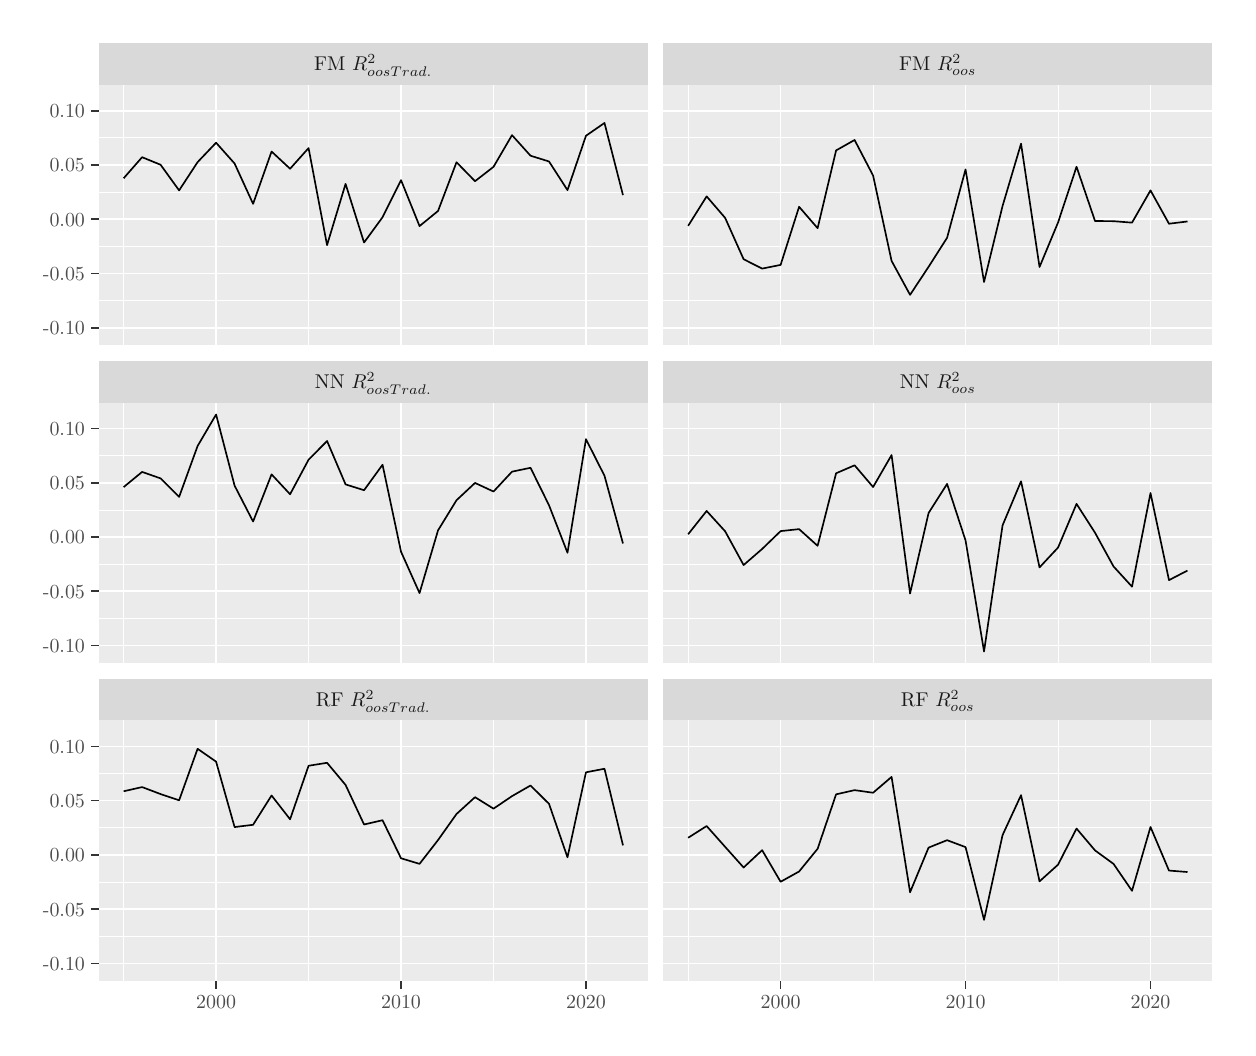
\begin{tikzpicture}[x=1pt,y=1pt]
\definecolor{fillColor}{RGB}{255,255,255}
\path[use as bounding box,fill=fillColor,fill opacity=0.00] (0,0) rectangle (433.62,361.35);
\begin{scope}
\path[clip] (  0.00,  0.00) rectangle (433.62,361.35);
\definecolor{drawColor}{RGB}{255,255,255}
\definecolor{fillColor}{RGB}{255,255,255}

\path[draw=drawColor,line width= 0.6pt,line join=round,line cap=round,fill=fillColor] (  0.00,  0.00) rectangle (433.62,361.35);
\end{scope}
\begin{scope}
\path[clip] ( 25.65,246.50) rectangle (224.13,340.69);
\definecolor{fillColor}{gray}{0.92}

\path[fill=fillColor] ( 25.65,246.50) rectangle (224.13,340.69);
\definecolor{drawColor}{RGB}{255,255,255}

\path[draw=drawColor,line width= 0.3pt,line join=round] ( 25.65,262.73) --
	(224.13,262.73);

\path[draw=drawColor,line width= 0.3pt,line join=round] ( 25.65,282.33) --
	(224.13,282.33);

\path[draw=drawColor,line width= 0.3pt,line join=round] ( 25.65,301.93) --
	(224.13,301.93);

\path[draw=drawColor,line width= 0.3pt,line join=round] ( 25.65,321.53) --
	(224.13,321.53);

\path[draw=drawColor,line width= 0.3pt,line join=round] ( 34.67,246.50) --
	( 34.67,340.69);

\path[draw=drawColor,line width= 0.3pt,line join=round] (101.50,246.50) --
	(101.50,340.69);

\path[draw=drawColor,line width= 0.3pt,line join=round] (168.33,246.50) --
	(168.33,340.69);

\path[draw=drawColor,line width= 0.6pt,line join=round] ( 25.65,252.92) --
	(224.13,252.92);

\path[draw=drawColor,line width= 0.6pt,line join=round] ( 25.65,272.53) --
	(224.13,272.53);

\path[draw=drawColor,line width= 0.6pt,line join=round] ( 25.65,292.13) --
	(224.13,292.13);

\path[draw=drawColor,line width= 0.6pt,line join=round] ( 25.65,311.73) --
	(224.13,311.73);

\path[draw=drawColor,line width= 0.6pt,line join=round] ( 25.65,331.33) --
	(224.13,331.33);

\path[draw=drawColor,line width= 0.6pt,line join=round] ( 68.08,246.50) --
	( 68.08,340.69);

\path[draw=drawColor,line width= 0.6pt,line join=round] (134.91,246.50) --
	(134.91,340.69);

\path[draw=drawColor,line width= 0.6pt,line join=round] (201.74,246.50) --
	(201.74,340.69);
\definecolor{drawColor}{RGB}{0,0,0}

\path[draw=drawColor,line width= 0.6pt,line join=round] ( 34.67,306.92) --
	( 41.35,314.54) --
	( 48.03,311.81) --
	( 54.72,302.55) --
	( 61.40,312.76) --
	( 68.08,319.77) --
	( 74.77,312.26) --
	( 81.45,297.68) --
	( 88.13,316.59) --
	( 94.82,310.37) --
	(101.50,317.84) --
	(108.18,282.78) --
	(114.87,304.90) --
	(121.55,283.71) --
	(128.23,292.84) --
	(134.91,306.26) --
	(141.60,289.65) --
	(148.28,295.11) --
	(154.96,312.72) --
	(161.65,305.87) --
	(168.33,311.06) --
	(175.01,322.51) --
	(181.70,315.08) --
	(188.38,313.00) --
	(195.06,302.65) --
	(201.74,322.29) --
	(208.43,326.91) --
	(215.11,300.85);
\end{scope}
\begin{scope}
\path[clip] ( 25.65,131.66) rectangle (224.13,225.84);
\definecolor{fillColor}{gray}{0.92}

\path[fill=fillColor] ( 25.65,131.66) rectangle (224.13,225.84);
\definecolor{drawColor}{RGB}{255,255,255}

\path[draw=drawColor,line width= 0.3pt,line join=round] ( 25.65,147.88) --
	(224.13,147.88);

\path[draw=drawColor,line width= 0.3pt,line join=round] ( 25.65,167.48) --
	(224.13,167.48);

\path[draw=drawColor,line width= 0.3pt,line join=round] ( 25.65,187.08) --
	(224.13,187.08);

\path[draw=drawColor,line width= 0.3pt,line join=round] ( 25.65,206.68) --
	(224.13,206.68);

\path[draw=drawColor,line width= 0.3pt,line join=round] ( 34.67,131.66) --
	( 34.67,225.84);

\path[draw=drawColor,line width= 0.3pt,line join=round] (101.50,131.66) --
	(101.50,225.84);

\path[draw=drawColor,line width= 0.3pt,line join=round] (168.33,131.66) --
	(168.33,225.84);

\path[draw=drawColor,line width= 0.6pt,line join=round] ( 25.65,138.08) --
	(224.13,138.08);

\path[draw=drawColor,line width= 0.6pt,line join=round] ( 25.65,157.68) --
	(224.13,157.68);

\path[draw=drawColor,line width= 0.6pt,line join=round] ( 25.65,177.28) --
	(224.13,177.28);

\path[draw=drawColor,line width= 0.6pt,line join=round] ( 25.65,196.88) --
	(224.13,196.88);

\path[draw=drawColor,line width= 0.6pt,line join=round] ( 25.65,216.49) --
	(224.13,216.49);

\path[draw=drawColor,line width= 0.6pt,line join=round] ( 68.08,131.66) --
	( 68.08,225.84);

\path[draw=drawColor,line width= 0.6pt,line join=round] (134.91,131.66) --
	(134.91,225.84);

\path[draw=drawColor,line width= 0.6pt,line join=round] (201.74,131.66) --
	(201.74,225.84);
\definecolor{drawColor}{RGB}{0,0,0}

\path[draw=drawColor,line width= 0.6pt,line join=round] ( 34.67,195.33) --
	( 41.35,200.82) --
	( 48.03,198.48) --
	( 54.72,191.78) --
	( 61.40,210.18) --
	( 68.08,221.56) --
	( 74.77,195.85) --
	( 81.45,182.90) --
	( 88.13,199.93) --
	( 94.82,192.75) --
	(101.50,205.22) --
	(108.18,211.99) --
	(114.87,196.31) --
	(121.55,194.21) --
	(128.23,203.41) --
	(134.91,171.98) --
	(141.60,157.04) --
	(148.28,179.70) --
	(154.96,190.59) --
	(161.65,196.84) --
	(168.33,193.73) --
	(175.01,200.91) --
	(181.70,202.31) --
	(188.38,188.78) --
	(195.06,171.61) --
	(201.74,212.64) --
	(208.43,199.43) --
	(215.11,174.97);
\end{scope}
\begin{scope}
\path[clip] ( 25.65, 16.81) rectangle (224.13,111.00);
\definecolor{fillColor}{gray}{0.92}

\path[fill=fillColor] ( 25.65, 16.81) rectangle (224.13,111.00);
\definecolor{drawColor}{RGB}{255,255,255}

\path[draw=drawColor,line width= 0.3pt,line join=round] ( 25.65, 33.03) --
	(224.13, 33.03);

\path[draw=drawColor,line width= 0.3pt,line join=round] ( 25.65, 52.63) --
	(224.13, 52.63);

\path[draw=drawColor,line width= 0.3pt,line join=round] ( 25.65, 72.24) --
	(224.13, 72.24);

\path[draw=drawColor,line width= 0.3pt,line join=round] ( 25.65, 91.84) --
	(224.13, 91.84);

\path[draw=drawColor,line width= 0.3pt,line join=round] ( 34.67, 16.81) --
	( 34.67,111.00);

\path[draw=drawColor,line width= 0.3pt,line join=round] (101.50, 16.81) --
	(101.50,111.00);

\path[draw=drawColor,line width= 0.3pt,line join=round] (168.33, 16.81) --
	(168.33,111.00);

\path[draw=drawColor,line width= 0.6pt,line join=round] ( 25.65, 23.23) --
	(224.13, 23.23);

\path[draw=drawColor,line width= 0.6pt,line join=round] ( 25.65, 42.83) --
	(224.13, 42.83);

\path[draw=drawColor,line width= 0.6pt,line join=round] ( 25.65, 62.43) --
	(224.13, 62.43);

\path[draw=drawColor,line width= 0.6pt,line join=round] ( 25.65, 82.04) --
	(224.13, 82.04);

\path[draw=drawColor,line width= 0.6pt,line join=round] ( 25.65,101.64) --
	(224.13,101.64);

\path[draw=drawColor,line width= 0.6pt,line join=round] ( 68.08, 16.81) --
	( 68.08,111.00);

\path[draw=drawColor,line width= 0.6pt,line join=round] (134.91, 16.81) --
	(134.91,111.00);

\path[draw=drawColor,line width= 0.6pt,line join=round] (201.74, 16.81) --
	(201.74,111.00);
\definecolor{drawColor}{RGB}{0,0,0}

\path[draw=drawColor,line width= 0.6pt,line join=round] ( 34.67, 85.42) --
	( 41.35, 86.94) --
	( 48.03, 84.41) --
	( 54.72, 82.15) --
	( 61.40,100.77) --
	( 68.08, 96.13) --
	( 74.77, 72.49) --
	( 81.45, 73.31) --
	( 88.13, 83.90) --
	( 94.82, 75.30) --
	(101.50, 94.64) --
	(108.18, 95.71) --
	(114.87, 87.71) --
	(121.55, 73.42) --
	(128.23, 74.96) --
	(134.91, 61.21) --
	(141.60, 59.19) --
	(148.28, 67.79) --
	(154.96, 77.21) --
	(161.65, 83.29) --
	(168.33, 79.14) --
	(175.01, 83.66) --
	(181.70, 87.51) --
	(188.38, 80.89) --
	(195.06, 61.56) --
	(201.74, 92.28) --
	(208.43, 93.56) --
	(215.11, 65.89);
\end{scope}
\begin{scope}
\path[clip] (229.63,246.50) rectangle (428.12,340.69);
\definecolor{fillColor}{gray}{0.92}

\path[fill=fillColor] (229.63,246.50) rectangle (428.12,340.69);
\definecolor{drawColor}{RGB}{255,255,255}

\path[draw=drawColor,line width= 0.3pt,line join=round] (229.63,262.73) --
	(428.12,262.73);

\path[draw=drawColor,line width= 0.3pt,line join=round] (229.63,282.33) --
	(428.12,282.33);

\path[draw=drawColor,line width= 0.3pt,line join=round] (229.63,301.93) --
	(428.12,301.93);

\path[draw=drawColor,line width= 0.3pt,line join=round] (229.63,321.53) --
	(428.12,321.53);

\path[draw=drawColor,line width= 0.3pt,line join=round] (238.66,246.50) --
	(238.66,340.69);

\path[draw=drawColor,line width= 0.3pt,line join=round] (305.49,246.50) --
	(305.49,340.69);

\path[draw=drawColor,line width= 0.3pt,line join=round] (372.32,246.50) --
	(372.32,340.69);

\path[draw=drawColor,line width= 0.6pt,line join=round] (229.63,252.92) --
	(428.12,252.92);

\path[draw=drawColor,line width= 0.6pt,line join=round] (229.63,272.53) --
	(428.12,272.53);

\path[draw=drawColor,line width= 0.6pt,line join=round] (229.63,292.13) --
	(428.12,292.13);

\path[draw=drawColor,line width= 0.6pt,line join=round] (229.63,311.73) --
	(428.12,311.73);

\path[draw=drawColor,line width= 0.6pt,line join=round] (229.63,331.33) --
	(428.12,331.33);

\path[draw=drawColor,line width= 0.6pt,line join=round] (272.07,246.50) --
	(272.07,340.69);

\path[draw=drawColor,line width= 0.6pt,line join=round] (338.90,246.50) --
	(338.90,340.69);

\path[draw=drawColor,line width= 0.6pt,line join=round] (405.73,246.50) --
	(405.73,340.69);
\definecolor{drawColor}{RGB}{0,0,0}

\path[draw=drawColor,line width= 0.6pt,line join=round] (238.66,289.74) --
	(245.34,300.38) --
	(252.02,292.62) --
	(258.70,277.68) --
	(265.39,274.28) --
	(272.07,275.62) --
	(278.75,296.62) --
	(285.44,288.89) --
	(292.12,316.99) --
	(298.80,320.76) --
	(305.49,307.91) --
	(312.17,277.07) --
	(318.85,264.81) --
	(325.54,274.93) --
	(332.22,285.41) --
	(338.90,310.13) --
	(345.58,269.46) --
	(352.27,296.91) --
	(358.95,319.42) --
	(365.63,274.87) --
	(372.32,290.94) --
	(379.00,311.09) --
	(385.68,291.49) --
	(392.37,291.42) --
	(399.05,290.89) --
	(405.73,302.54) --
	(412.41,290.50) --
	(419.10,291.32);
\end{scope}
\begin{scope}
\path[clip] (229.63,131.66) rectangle (428.12,225.84);
\definecolor{fillColor}{gray}{0.92}

\path[fill=fillColor] (229.63,131.66) rectangle (428.12,225.84);
\definecolor{drawColor}{RGB}{255,255,255}

\path[draw=drawColor,line width= 0.3pt,line join=round] (229.63,147.88) --
	(428.12,147.88);

\path[draw=drawColor,line width= 0.3pt,line join=round] (229.63,167.48) --
	(428.12,167.48);

\path[draw=drawColor,line width= 0.3pt,line join=round] (229.63,187.08) --
	(428.12,187.08);

\path[draw=drawColor,line width= 0.3pt,line join=round] (229.63,206.68) --
	(428.12,206.68);

\path[draw=drawColor,line width= 0.3pt,line join=round] (238.66,131.66) --
	(238.66,225.84);

\path[draw=drawColor,line width= 0.3pt,line join=round] (305.49,131.66) --
	(305.49,225.84);

\path[draw=drawColor,line width= 0.3pt,line join=round] (372.32,131.66) --
	(372.32,225.84);

\path[draw=drawColor,line width= 0.6pt,line join=round] (229.63,138.08) --
	(428.12,138.08);

\path[draw=drawColor,line width= 0.6pt,line join=round] (229.63,157.68) --
	(428.12,157.68);

\path[draw=drawColor,line width= 0.6pt,line join=round] (229.63,177.28) --
	(428.12,177.28);

\path[draw=drawColor,line width= 0.6pt,line join=round] (229.63,196.88) --
	(428.12,196.88);

\path[draw=drawColor,line width= 0.6pt,line join=round] (229.63,216.49) --
	(428.12,216.49);

\path[draw=drawColor,line width= 0.6pt,line join=round] (272.07,131.66) --
	(272.07,225.84);

\path[draw=drawColor,line width= 0.6pt,line join=round] (338.90,131.66) --
	(338.90,225.84);

\path[draw=drawColor,line width= 0.6pt,line join=round] (405.73,131.66) --
	(405.73,225.84);
\definecolor{drawColor}{RGB}{0,0,0}

\path[draw=drawColor,line width= 0.6pt,line join=round] (238.66,178.30) --
	(245.34,186.71) --
	(252.02,179.37) --
	(258.70,167.17) --
	(265.39,172.97) --
	(272.07,179.43) --
	(278.75,180.15) --
	(285.44,174.11) --
	(292.12,200.33) --
	(298.80,203.21) --
	(305.49,195.36) --
	(312.17,206.91) --
	(318.85,156.89) --
	(325.54,185.98) --
	(332.22,196.47) --
	(338.90,176.05) --
	(345.58,135.94) --
	(352.27,181.50) --
	(358.95,197.43) --
	(365.63,166.32) --
	(372.32,173.48) --
	(379.00,189.27) --
	(385.68,178.85) --
	(392.37,166.66) --
	(399.05,159.35) --
	(405.73,193.18) --
	(412.41,161.72) --
	(419.10,165.18);
\end{scope}
\begin{scope}
\path[clip] (229.63, 16.81) rectangle (428.12,111.00);
\definecolor{fillColor}{gray}{0.92}

\path[fill=fillColor] (229.63, 16.81) rectangle (428.12,111.00);
\definecolor{drawColor}{RGB}{255,255,255}

\path[draw=drawColor,line width= 0.3pt,line join=round] (229.63, 33.03) --
	(428.12, 33.03);

\path[draw=drawColor,line width= 0.3pt,line join=round] (229.63, 52.63) --
	(428.12, 52.63);

\path[draw=drawColor,line width= 0.3pt,line join=round] (229.63, 72.24) --
	(428.12, 72.24);

\path[draw=drawColor,line width= 0.3pt,line join=round] (229.63, 91.84) --
	(428.12, 91.84);

\path[draw=drawColor,line width= 0.3pt,line join=round] (238.66, 16.81) --
	(238.66,111.00);

\path[draw=drawColor,line width= 0.3pt,line join=round] (305.49, 16.81) --
	(305.49,111.00);

\path[draw=drawColor,line width= 0.3pt,line join=round] (372.32, 16.81) --
	(372.32,111.00);

\path[draw=drawColor,line width= 0.6pt,line join=round] (229.63, 23.23) --
	(428.12, 23.23);

\path[draw=drawColor,line width= 0.6pt,line join=round] (229.63, 42.83) --
	(428.12, 42.83);

\path[draw=drawColor,line width= 0.6pt,line join=round] (229.63, 62.43) --
	(428.12, 62.43);

\path[draw=drawColor,line width= 0.6pt,line join=round] (229.63, 82.04) --
	(428.12, 82.04);

\path[draw=drawColor,line width= 0.6pt,line join=round] (229.63,101.64) --
	(428.12,101.64);

\path[draw=drawColor,line width= 0.6pt,line join=round] (272.07, 16.81) --
	(272.07,111.00);

\path[draw=drawColor,line width= 0.6pt,line join=round] (338.90, 16.81) --
	(338.90,111.00);

\path[draw=drawColor,line width= 0.6pt,line join=round] (405.73, 16.81) --
	(405.73,111.00);
\definecolor{drawColor}{RGB}{0,0,0}

\path[draw=drawColor,line width= 0.6pt,line join=round] (238.66, 68.62) --
	(245.34, 72.86) --
	(252.02, 65.34) --
	(258.70, 57.88) --
	(265.39, 64.13) --
	(272.07, 52.72) --
	(278.75, 56.43) --
	(285.44, 64.64) --
	(292.12, 84.31) --
	(298.80, 85.83) --
	(305.49, 84.89) --
	(312.17, 90.61) --
	(318.85, 48.94) --
	(325.54, 65.06) --
	(332.22, 67.75) --
	(338.90, 65.24) --
	(345.58, 38.96) --
	(352.27, 69.58) --
	(358.95, 84.01) --
	(365.63, 52.87) --
	(372.32, 58.90) --
	(379.00, 71.95) --
	(385.68, 64.06) --
	(392.37, 59.18) --
	(399.05, 49.45) --
	(405.73, 72.52) --
	(412.41, 56.77) --
	(419.10, 56.24);
\end{scope}
\begin{scope}
\path[clip] ( 25.65,111.00) rectangle (224.13,126.16);
\definecolor{fillColor}{gray}{0.85}

\path[fill=fillColor] ( 25.65,111.00) rectangle (224.13,126.16);
\definecolor{drawColor}{gray}{0.10}

\node[text=drawColor,anchor=base,inner sep=0pt, outer sep=0pt, scale=  0.72] at (124.89,116.10) {RF $R^2_{oos  Trad.}$};
\end{scope}
\begin{scope}
\path[clip] (229.63,111.00) rectangle (428.12,126.16);
\definecolor{fillColor}{gray}{0.85}

\path[fill=fillColor] (229.63,111.00) rectangle (428.12,126.16);
\definecolor{drawColor}{gray}{0.10}

\node[text=drawColor,anchor=base,inner sep=0pt, outer sep=0pt, scale=  0.72] at (328.88,116.10) {RF $R^2_{oos}$};
\end{scope}
\begin{scope}
\path[clip] ( 25.65,225.84) rectangle (224.13,241.00);
\definecolor{fillColor}{gray}{0.85}

\path[fill=fillColor] ( 25.65,225.84) rectangle (224.13,241.00);
\definecolor{drawColor}{gray}{0.10}

\node[text=drawColor,anchor=base,inner sep=0pt, outer sep=0pt, scale=  0.72] at (124.89,230.94) {NN $R^2_{oos  Trad.}$};
\end{scope}
\begin{scope}
\path[clip] (229.63,225.84) rectangle (428.12,241.00);
\definecolor{fillColor}{gray}{0.85}

\path[fill=fillColor] (229.63,225.84) rectangle (428.12,241.00);
\definecolor{drawColor}{gray}{0.10}

\node[text=drawColor,anchor=base,inner sep=0pt, outer sep=0pt, scale=  0.72] at (328.88,230.94) {NN $R^2_{oos}$};
\end{scope}
\begin{scope}
\path[clip] ( 25.65,340.69) rectangle (224.13,355.85);
\definecolor{fillColor}{gray}{0.85}

\path[fill=fillColor] ( 25.65,340.69) rectangle (224.13,355.85);
\definecolor{drawColor}{gray}{0.10}

\node[text=drawColor,anchor=base,inner sep=0pt, outer sep=0pt, scale=  0.72] at (124.89,345.79) {FM $R^2_{oos  Trad.}$};
\end{scope}
\begin{scope}
\path[clip] (229.63,340.69) rectangle (428.12,355.85);
\definecolor{fillColor}{gray}{0.85}

\path[fill=fillColor] (229.63,340.69) rectangle (428.12,355.85);
\definecolor{drawColor}{gray}{0.10}

\node[text=drawColor,anchor=base,inner sep=0pt, outer sep=0pt, scale=  0.72] at (328.88,345.79) {FM $R^2_{oos}$};
\end{scope}
\begin{scope}
\path[clip] (  0.00,  0.00) rectangle (433.62,361.35);
\definecolor{drawColor}{gray}{0.20}

\path[draw=drawColor,line width= 0.6pt,line join=round] ( 68.08, 14.06) --
	( 68.08, 16.81);

\path[draw=drawColor,line width= 0.6pt,line join=round] (134.91, 14.06) --
	(134.91, 16.81);

\path[draw=drawColor,line width= 0.6pt,line join=round] (201.74, 14.06) --
	(201.74, 16.81);
\end{scope}
\begin{scope}
\path[clip] (  0.00,  0.00) rectangle (433.62,361.35);
\definecolor{drawColor}{gray}{0.30}

\node[text=drawColor,anchor=base,inner sep=0pt, outer sep=0pt, scale=  0.72] at ( 68.08,  6.90) {2000};

\node[text=drawColor,anchor=base,inner sep=0pt, outer sep=0pt, scale=  0.72] at (134.91,  6.90) {2010};

\node[text=drawColor,anchor=base,inner sep=0pt, outer sep=0pt, scale=  0.72] at (201.74,  6.90) {2020};
\end{scope}
\begin{scope}
\path[clip] (  0.00,  0.00) rectangle (433.62,361.35);
\definecolor{drawColor}{gray}{0.20}

\path[draw=drawColor,line width= 0.6pt,line join=round] (272.07, 14.06) --
	(272.07, 16.81);

\path[draw=drawColor,line width= 0.6pt,line join=round] (338.90, 14.06) --
	(338.90, 16.81);

\path[draw=drawColor,line width= 0.6pt,line join=round] (405.73, 14.06) --
	(405.73, 16.81);
\end{scope}
\begin{scope}
\path[clip] (  0.00,  0.00) rectangle (433.62,361.35);
\definecolor{drawColor}{gray}{0.30}

\node[text=drawColor,anchor=base,inner sep=0pt, outer sep=0pt, scale=  0.72] at (272.07,  6.90) {2000};

\node[text=drawColor,anchor=base,inner sep=0pt, outer sep=0pt, scale=  0.72] at (338.90,  6.90) {2010};

\node[text=drawColor,anchor=base,inner sep=0pt, outer sep=0pt, scale=  0.72] at (405.73,  6.90) {2020};
\end{scope}
\begin{scope}
\path[clip] (  0.00,  0.00) rectangle (433.62,361.35);
\definecolor{drawColor}{gray}{0.30}

\node[text=drawColor,anchor=base east,inner sep=0pt, outer sep=0pt, scale=  0.72] at ( 20.70,250.44) {-0.10};

\node[text=drawColor,anchor=base east,inner sep=0pt, outer sep=0pt, scale=  0.72] at ( 20.70,270.05) {-0.05};

\node[text=drawColor,anchor=base east,inner sep=0pt, outer sep=0pt, scale=  0.72] at ( 20.70,289.65) {0.00};

\node[text=drawColor,anchor=base east,inner sep=0pt, outer sep=0pt, scale=  0.72] at ( 20.70,309.25) {0.05};

\node[text=drawColor,anchor=base east,inner sep=0pt, outer sep=0pt, scale=  0.72] at ( 20.70,328.85) {0.10};
\end{scope}
\begin{scope}
\path[clip] (  0.00,  0.00) rectangle (433.62,361.35);
\definecolor{drawColor}{gray}{0.20}

\path[draw=drawColor,line width= 0.6pt,line join=round] ( 22.90,252.92) --
	( 25.65,252.92);

\path[draw=drawColor,line width= 0.6pt,line join=round] ( 22.90,272.53) --
	( 25.65,272.53);

\path[draw=drawColor,line width= 0.6pt,line join=round] ( 22.90,292.13) --
	( 25.65,292.13);

\path[draw=drawColor,line width= 0.6pt,line join=round] ( 22.90,311.73) --
	( 25.65,311.73);

\path[draw=drawColor,line width= 0.6pt,line join=round] ( 22.90,331.33) --
	( 25.65,331.33);
\end{scope}
\begin{scope}
\path[clip] (  0.00,  0.00) rectangle (433.62,361.35);
\definecolor{drawColor}{gray}{0.30}

\node[text=drawColor,anchor=base east,inner sep=0pt, outer sep=0pt, scale=  0.72] at ( 20.70,135.60) {-0.10};

\node[text=drawColor,anchor=base east,inner sep=0pt, outer sep=0pt, scale=  0.72] at ( 20.70,155.20) {-0.05};

\node[text=drawColor,anchor=base east,inner sep=0pt, outer sep=0pt, scale=  0.72] at ( 20.70,174.80) {0.00};

\node[text=drawColor,anchor=base east,inner sep=0pt, outer sep=0pt, scale=  0.72] at ( 20.70,194.40) {0.05};

\node[text=drawColor,anchor=base east,inner sep=0pt, outer sep=0pt, scale=  0.72] at ( 20.70,214.01) {0.10};
\end{scope}
\begin{scope}
\path[clip] (  0.00,  0.00) rectangle (433.62,361.35);
\definecolor{drawColor}{gray}{0.20}

\path[draw=drawColor,line width= 0.6pt,line join=round] ( 22.90,138.08) --
	( 25.65,138.08);

\path[draw=drawColor,line width= 0.6pt,line join=round] ( 22.90,157.68) --
	( 25.65,157.68);

\path[draw=drawColor,line width= 0.6pt,line join=round] ( 22.90,177.28) --
	( 25.65,177.28);

\path[draw=drawColor,line width= 0.6pt,line join=round] ( 22.90,196.88) --
	( 25.65,196.88);

\path[draw=drawColor,line width= 0.6pt,line join=round] ( 22.90,216.49) --
	( 25.65,216.49);
\end{scope}
\begin{scope}
\path[clip] (  0.00,  0.00) rectangle (433.62,361.35);
\definecolor{drawColor}{gray}{0.30}

\node[text=drawColor,anchor=base east,inner sep=0pt, outer sep=0pt, scale=  0.72] at ( 20.70, 20.75) {-0.10};

\node[text=drawColor,anchor=base east,inner sep=0pt, outer sep=0pt, scale=  0.72] at ( 20.70, 40.35) {-0.05};

\node[text=drawColor,anchor=base east,inner sep=0pt, outer sep=0pt, scale=  0.72] at ( 20.70, 59.95) {0.00};

\node[text=drawColor,anchor=base east,inner sep=0pt, outer sep=0pt, scale=  0.72] at ( 20.70, 79.56) {0.05};

\node[text=drawColor,anchor=base east,inner sep=0pt, outer sep=0pt, scale=  0.72] at ( 20.70, 99.16) {0.10};
\end{scope}
\begin{scope}
\path[clip] (  0.00,  0.00) rectangle (433.62,361.35);
\definecolor{drawColor}{gray}{0.20}

\path[draw=drawColor,line width= 0.6pt,line join=round] ( 22.90, 23.23) --
	( 25.65, 23.23);

\path[draw=drawColor,line width= 0.6pt,line join=round] ( 22.90, 42.83) --
	( 25.65, 42.83);

\path[draw=drawColor,line width= 0.6pt,line join=round] ( 22.90, 62.43) --
	( 25.65, 62.43);

\path[draw=drawColor,line width= 0.6pt,line join=round] ( 22.90, 82.04) --
	( 25.65, 82.04);

\path[draw=drawColor,line width= 0.6pt,line join=round] ( 22.90,101.64) --
	( 25.65,101.64);
\end{scope}
\end{tikzpicture}

\label{plot:OOSR2_ts}
\end{figure}

\section{Benchmark factors}
\renewcommand{\thefigure}{B.\arabic{figure}}
\setcounter{figure}{0}
\renewcommand{\thetable}{B.\arabic{table}}
\setcounter{table}{0}

Benchmark factor construction follows $2 \times 3$ portfolio sort approach of Fama and French \citeyear{FAMA19933, FAMA20151} and Carhart \citeyear{Carhart1997}. Fama and French \citeyear{FAMA19933} use NYSE breakpoints for size and book-to-market value sort. Since on compared to US markets Nordic markets have less companies with high market value. Using NYSE breakpoints could lead to highly un-diversified portfolios especially among the high market value portfolios. On the other hand breakpoints should not be driven by the small stocks that are numerous, but only account for small part of the total market capitalization. Therefore approach of Fama and French \citeyear{FAMA2012457} is applied. 

In the end of each June stocks are first distributed to two size portfolios. Companies with biggest market value that account for $90\%$ total market value are classified as big stocks. All the rest of the stocks are considered to be small stocks. Next stocks are allocated to three value, investment, profitability and momentum portfolios. For all of above variables 30th and 70th percentiles are used to calculate breakpoints. Breakpoints are calculated using only big companies from the size allocation, but the breakpoints are used to allocate all stocks to a portfolio.

\begin{equation} \label{eq:FF6factors}
\begin{split}
SMB_{B/M} = & \ \frac{1}{3} (Small.High + Small.Neutral + Small.Low) \\
			& - \frac{1}{3} (Big.High + Big.Neutral + Big.Low) \\[5pt]
SMB_{OP} = & \ \frac{1}{3} (Small.Robust + Small.Neutral_{OP} + Small.Weak)\\
			& - \frac{1}{3} (Big.Robust + Big.Neutral_{OP} + Big.Weak)\\[5pt]
SMB_{INV} = & \ \frac{1}{3} (Small.Conservative + Small.Neutral_{INV} + Small.Aggressive)\\
			& - \frac{1}{3} (Big.Conservative + Big.Neutral_{INV} + Big.Aggressive)\\[5pt]
SMB_{MOM} = & \ \frac{1}{3} ((Small.Winner + Small.Neutral_{MOM} + Small.Loser)\\
		     	& - \frac{1}{3} (Big.Winner + Big.Neutral_{MOM} + Big.Loser)\\[5pt]
SMB = & \ \frac{1}{4} (SMB_{B/M} + SMB_{OP} + SMB_{INV} + SMB_{MOM})\\[20pt]
HML = & \ \frac{1}{2} (Small.High + Big.High) - \frac{1}{2} (Small.Low + Big.Low)\\[5pt]
RMW = & \ \frac{1}{2} (Small.Robust + Big.Robust) - \frac{1}{2} (Small.Weak + Big.Weak)\\[5pt]
CMA = & \ \frac{1}{2} (Small.Conservative + Big.Conservative)\\
		& - \frac{1}{2} (Small.Aggressive + Big.Aggressive)
\end{split}
\end{equation}

Book-to-market value is used as indicator of value characteristic of a company. Book-to-market value is calculated as ratio between sum of common equity and deferred taxes and market capitalization on December $t-1$. Profitability is defined as net income before extra items/preferred dividends divided by the book equity of the company. Investment variable is calculated as annual change in total assets. Momentum is defined as cumulated return from $t-12$ to $t-2$. Returns are calculated using total return index that is converted to US dollars for comparability between different countries. Market value used in size allocation as well as to weight portfolio returns is also converted to US dollars. 

\begin{figure}[h]
\centering
\caption[Benchmark factor performance]{\textbf{Benchmark factor performance}\\ Plot presents the cumulative return of the benchmark factors. RMRF is average value weighted excess return of pooled Nordic market. Portfolio returns are calculated based on $2 \times 3$ sorts on size and one other factor. HML is the difference in average of value weighted return of two high value portfolios and average of value weighted return of two low value portfolios. RMW, CMA and MOM are calculated in similar manner, but portfolio sort are done based on investment, profitability momentum factors. SMB is the average of the value weighted returns of the 12 portfolios of small stocks minus the average of the value weighted returns of the 12 portfolios of big stocks. Returns are calculated in US dollars.}
% Created by tikzDevice version 0.12.6 on 2024-03-02 18:23:12
% !TEX encoding = UTF-8 Unicode
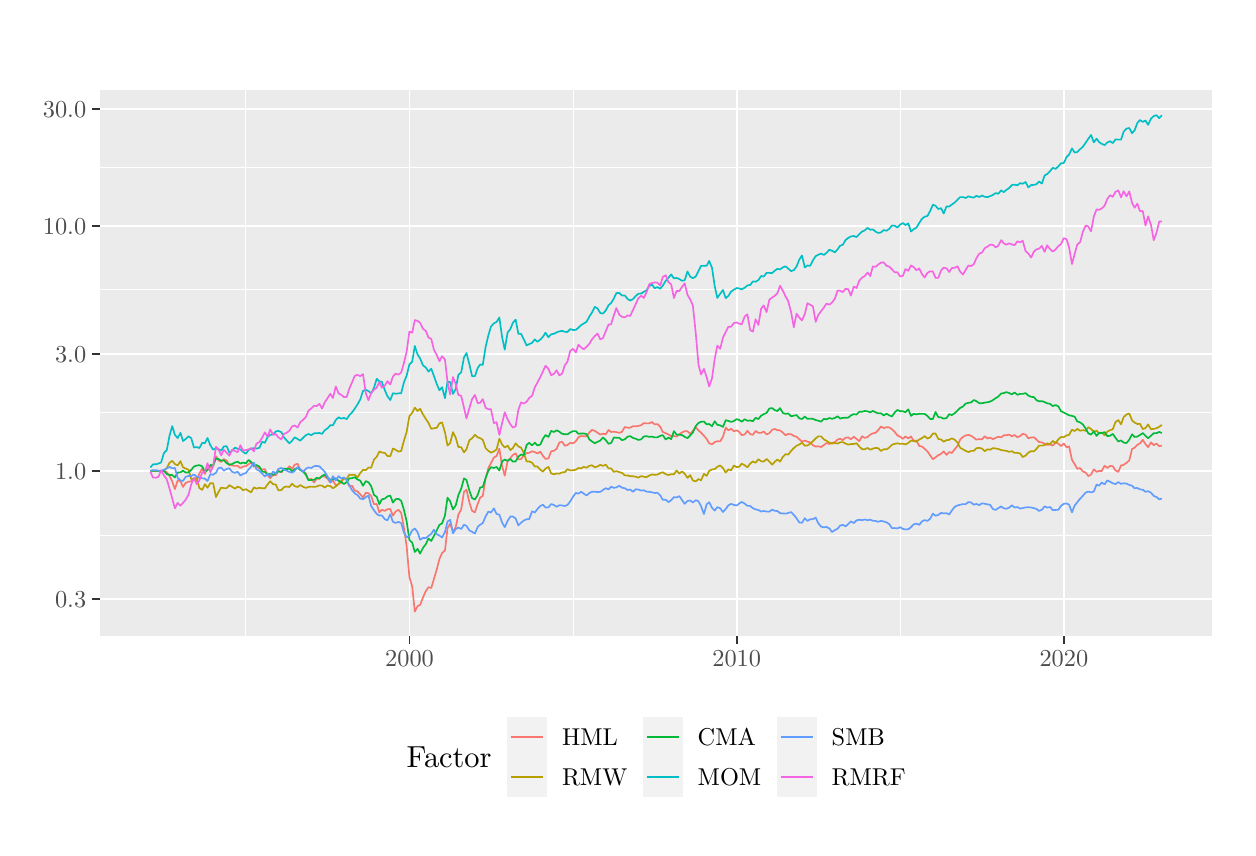
\begin{tikzpicture}[x=1pt,y=1pt]
\definecolor{fillColor}{RGB}{255,255,255}
\path[use as bounding box,fill=fillColor,fill opacity=0.00] (0,0) rectangle (433.62,289.08);
\begin{scope}
\path[clip] (  0.00,  0.00) rectangle (433.62,289.08);
\definecolor{drawColor}{RGB}{255,255,255}
\definecolor{fillColor}{RGB}{255,255,255}

\path[draw=drawColor,line width= 0.6pt,line join=round,line cap=round,fill=fillColor] (  0.00,  0.00) rectangle (433.62,289.08);
\end{scope}
\begin{scope}
\path[clip] ( 26.09, 69.13) rectangle (428.12,266.42);
\definecolor{fillColor}{gray}{0.92}

\path[fill=fillColor] ( 26.09, 69.13) rectangle (428.12,266.42);
\definecolor{drawColor}{RGB}{255,255,255}

\path[draw=drawColor,line width= 0.3pt,line join=round] ( 26.09,105.77) --
	(428.12,105.77);

\path[draw=drawColor,line width= 0.3pt,line join=round] ( 26.09,150.06) --
	(428.12,150.06);

\path[draw=drawColor,line width= 0.3pt,line join=round] ( 26.09,194.35) --
	(428.12,194.35);

\path[draw=drawColor,line width= 0.3pt,line join=round] ( 26.09,238.64) --
	(428.12,238.64);

\path[draw=drawColor,line width= 0.3pt,line join=round] ( 78.85, 69.13) --
	( 78.85,266.42);

\path[draw=drawColor,line width= 0.3pt,line join=round] (197.10, 69.13) --
	(197.10,266.42);

\path[draw=drawColor,line width= 0.3pt,line join=round] (315.33, 69.13) --
	(315.33,266.42);

\path[draw=drawColor,line width= 0.6pt,line join=round] ( 26.09, 82.61) --
	(428.12, 82.61);

\path[draw=drawColor,line width= 0.6pt,line join=round] ( 26.09,128.93) --
	(428.12,128.93);

\path[draw=drawColor,line width= 0.6pt,line join=round] ( 26.09,171.19) --
	(428.12,171.19);

\path[draw=drawColor,line width= 0.6pt,line join=round] ( 26.09,217.51) --
	(428.12,217.51);

\path[draw=drawColor,line width= 0.6pt,line join=round] ( 26.09,259.78) --
	(428.12,259.78);

\path[draw=drawColor,line width= 0.6pt,line join=round] (137.98, 69.13) --
	(137.98,266.42);

\path[draw=drawColor,line width= 0.6pt,line join=round] (256.22, 69.13) --
	(256.22,266.42);

\path[draw=drawColor,line width= 0.6pt,line join=round] (374.43, 69.13) --
	(374.43,266.42);
\definecolor{drawColor}{RGB}{248,118,109}

\path[draw=drawColor,line width= 0.6pt,line join=round] ( 44.36,128.93) --
	( 45.27,128.93) --
	( 46.31,128.93) --
	( 47.28,128.93) --
	( 48.22,128.93) --
	( 49.25,128.93) --
	( 50.26,128.46) --
	( 51.26,127.09) --
	( 52.23,125.08) --
	( 53.20,122.33) --
	( 54.21,125.52) --
	( 55.21,125.16) --
	( 56.15,123.12) --
	( 57.05,124.54) --
	( 58.12,125.01) --
	( 59.09,125.17) --
	( 60.10,126.01) --
	( 61.07,125.20) --
	( 62.04,127.96) --
	( 63.07,129.77) --
	( 64.05,127.77) --
	( 64.98,131.17) --
	( 66.02,130.12) --
	( 67.02,130.66) --
	( 68.03,134.25) --
	( 68.93,132.70) --
	( 69.94,132.19) --
	( 70.88,133.19) --
	( 71.91,132.62) --
	( 72.88,130.99) --
	( 73.82,130.91) --
	( 74.89,130.72) --
	( 75.86,130.72) --
	( 76.86,129.99) --
	( 77.83,130.47) --
	( 78.81,130.66) --
	( 79.84,131.32) --
	( 80.75,131.96) --
	( 81.75,130.45) --
	( 82.66,130.49) --
	( 83.73,129.85) --
	( 84.70,129.36) --
	( 85.70,129.59) --
	( 86.70,127.32) --
	( 87.64,126.29) --
	( 88.68,127.47) --
	( 89.65,127.34) --
	( 90.59,128.98) --
	( 91.66,128.41) --
	( 92.59,129.40) --
	( 93.53,129.44) --
	( 94.57,130.60) --
	( 95.57,129.69) --
	( 96.48,131.16) --
	( 97.55,131.47) --
	( 98.52,129.22) --
	( 99.52,128.93) --
	(100.53,127.99) --
	(101.46,125.66) --
	(102.50,126.09) --
	(103.50,124.71) --
	(104.41,126.06) --
	(105.41,126.05) --
	(106.38,126.96) --
	(107.36,126.89) --
	(108.36,126.11) --
	(109.36,124.68) --
	(110.30,125.42) --
	(111.34,123.69) --
	(112.34,124.18) --
	(113.25,124.66) --
	(114.31,126.48) --
	(115.29,125.60) --
	(116.19,123.45) --
	(117.23,123.55) --
	(118.20,121.74) --
	(119.14,121.57) --
	(120.17,120.47) --
	(121.18,119.32) --
	(122.18,121.00) --
	(123.15,120.85) --
	(124.12,119.81) --
	(125.13,116.88) --
	(126.13,116.96) --
	(127.07,113.92) --
	(127.97,114.87) --
	(129.04,114.45) --
	(130.01,115.11) --
	(131.02,115.13) --
	(131.99,112.73) --
	(132.96,114.27) --
	(134.00,114.89) --
	(134.97,113.71) --
	(135.90,108.72) --
	(136.94,101.67) --
	(137.94, 90.52) --
	(138.95, 87.15) --
	(139.89, 78.10) --
	(140.89, 80.09) --
	(141.80, 80.47) --
	(142.86, 83.21) --
	(143.84, 85.44) --
	(144.84, 86.89) --
	(145.84, 86.62) --
	(146.78, 89.77) --
	(147.82, 93.33) --
	(148.79, 97.08) --
	(149.73, 99.22) --
	(150.79,100.18) --
	(151.70,108.21) --
	(152.67,109.85) --
	(153.68,106.87) --
	(154.68,108.59) --
	(155.62,113.10) --
	(156.65,114.98) --
	(157.66,121.33) --
	(158.56,122.15) --
	(159.63,117.49) --
	(160.60,114.44) --
	(161.61,113.95) --
	(162.61,116.96) --
	(163.52,119.29) --
	(164.45,119.87) --
	(165.49,126.29) --
	(166.49,130.02) --
	(167.40,131.71) --
	(168.47,133.74) --
	(169.44,134.31) --
	(170.44,136.93) --
	(171.45,130.56) --
	(172.39,127.19) --
	(173.42,132.46) --
	(174.42,133.55) --
	(175.33,134.69) --
	(176.33,135.27) --
	(177.31,133.14) --
	(178.28,133.18) --
	(179.28,134.60) --
	(180.28,135.34) --
	(181.22,135.46) --
	(182.26,136.01) --
	(183.26,135.68) --
	(184.17,135.21) --
	(185.24,135.87) --
	(186.21,134.34) --
	(187.11,133.25) --
	(188.18,133.42) --
	(189.15,135.98) --
	(190.16,136.20) --
	(191.13,136.89) --
	(192.10,139.18) --
	(193.13,139.41) --
	(194.10,138.01) --
	(195.04,138.26) --
	(196.08,139.08) --
	(197.08,138.85) --
	(198.09,139.68) --
	(198.99,141.04) --
	(200.00,141.55) --
	(200.93,141.42) --
	(201.97,141.44) --
	(202.94,142.77) --
	(203.88,143.72) --
	(204.95,143.40) --
	(205.92,142.70) --
	(206.92,142.04) --
	(207.89,142.36) --
	(208.87,142.15) --
	(209.90,143.69) --
	(210.81,142.98) --
	(211.81,143.09) --
	(212.72,142.94) --
	(213.79,142.68) --
	(214.76,143.05) --
	(215.76,144.78) --
	(216.76,144.54) --
	(217.70,144.53) --
	(218.74,145.08) --
	(219.71,145.01) --
	(220.65,145.17) --
	(221.72,145.46) --
	(222.62,146.18) --
	(223.59,146.09) --
	(224.60,146.11) --
	(225.60,146.59) --
	(226.54,145.76) --
	(227.57,145.84) --
	(228.58,144.84) --
	(229.48,143.01) --
	(230.55,142.54) --
	(231.52,142.10) --
	(232.53,141.49) --
	(233.53,141.56) --
	(234.47,141.31) --
	(235.47,142.18) --
	(236.44,142.82) --
	(237.41,143.28) --
	(238.42,143.27) --
	(239.42,142.22) --
	(240.36,143.41) --
	(241.40,144.71) --
	(242.40,143.55) --
	(243.31,142.76) --
	(244.37,141.61) --
	(245.35,140.46) --
	(246.25,138.93) --
	(247.29,138.53) --
	(248.26,139.32) --
	(249.20,139.65) --
	(250.23,139.56) --
	(251.24,141.29) --
	(252.24,144.58) --
	(253.21,143.58) --
	(254.18,144.14) --
	(255.19,143.23) --
	(256.19,143.60) --
	(257.13,142.98) --
	(258.03,141.83) --
	(259.10,142.09) --
	(260.07,143.41) --
	(261.08,142.23) --
	(262.05,141.97) --
	(263.02,143.34) --
	(264.05,142.68) --
	(265.03,142.65) --
	(265.96,143.14) --
	(267.00,142.13) --
	(268.00,142.54) --
	(269.01,143.76) --
	(269.91,144.07) --
	(270.92,143.63) --
	(271.86,143.55) --
	(272.89,142.74) --
	(273.86,141.83) --
	(274.80,142.25) --
	(275.87,142.17) --
	(276.84,141.55) --
	(277.84,141.25) --
	(278.82,140.37) --
	(279.79,139.49) --
	(280.82,139.87) --
	(281.76,139.52) --
	(282.73,139.20) --
	(283.74,138.20) --
	(284.74,137.69) --
	(285.68,137.83) --
	(286.71,137.54) --
	(287.72,138.25) --
	(288.62,138.96) --
	(289.69,138.65) --
	(290.66,139.03) --
	(291.67,139.34) --
	(292.67,140.26) --
	(293.58,140.54) --
	(294.51,140.05) --
	(295.55,140.89) --
	(296.55,141.01) --
	(297.46,140.36) --
	(298.53,141.26) --
	(299.50,140.46) --
	(300.50,139.67) --
	(301.51,141.44) --
	(302.44,140.83) --
	(303.48,141.14) --
	(304.48,142.06) --
	(305.39,142.49) --
	(306.39,142.69) --
	(307.36,143.67) --
	(308.34,144.95) --
	(309.34,144.40) --
	(310.34,144.70) --
	(311.28,144.65) --
	(312.32,143.99) --
	(313.32,142.98) --
	(314.23,141.78) --
	(315.30,141.25) --
	(316.27,140.50) --
	(317.17,141.36) --
	(318.21,140.68) --
	(319.18,141.36) --
	(320.12,139.85) --
	(321.15,139.88) --
	(322.16,137.93) --
	(323.16,137.73) --
	(324.13,136.89) --
	(325.10,136.00) --
	(326.11,134.53) --
	(327.11,133.16) --
	(328.05,133.81) --
	(329.05,134.60) --
	(330.06,135.08) --
	(330.99,135.94) --
	(332.03,134.71) --
	(333.00,135.75) --
	(333.94,135.39) --
	(335.01,136.77) --
	(335.98,138.02) --
	(336.98,140.28) --
	(337.95,141.16) --
	(338.92,141.74) --
	(339.96,141.90) --
	(340.87,141.64) --
	(341.87,140.97) --
	(342.78,140.22) --
	(343.85,140.42) --
	(344.82,140.30) --
	(345.82,141.43) --
	(346.82,140.63) --
	(347.76,140.93) --
	(348.80,140.41) --
	(349.77,140.86) --
	(350.71,141.25) --
	(351.78,141.02) --
	(352.68,141.78) --
	(353.65,141.80) --
	(354.66,142.05) --
	(355.66,141.41) --
	(356.60,141.89) --
	(357.63,141.11) --
	(358.64,141.51) --
	(359.54,142.31) --
	(360.61,142.03) --
	(361.58,140.70) --
	(362.59,140.99) --
	(363.59,141.06) --
	(364.50,140.27) --
	(365.44,139.37) --
	(366.47,139.24) --
	(367.47,138.75) --
	(368.38,138.33) --
	(369.45,138.45) --
	(370.42,138.06) --
	(371.42,139.21) --
	(372.43,138.76) --
	(373.37,137.90) --
	(374.40,138.80) --
	(375.41,137.44) --
	(376.31,137.79) --
	(377.35,132.93) --
	(378.32,131.35) --
	(379.26,129.67) --
	(380.29,129.95) --
	(381.30,128.69) --
	(382.30,128.32) --
	(383.27,127.04) --
	(384.24,127.58) --
	(385.25,129.49) --
	(386.25,128.58) --
	(387.19,128.93) --
	(388.09,128.87) --
	(389.16,130.81) --
	(390.13,129.99) --
	(391.14,130.70) --
	(392.11,130.60) --
	(393.08,129.08) --
	(394.11,128.61) --
	(395.09,130.90) --
	(396.02,131.10) --
	(397.06,131.83) --
	(398.06,132.70) --
	(399.07,136.88) --
	(399.97,137.26) --
	(400.98,138.34) --
	(401.92,138.85) --
	(402.95,140.16) --
	(403.92,138.63) --
	(404.86,137.49) --
	(405.93,139.21) --
	(406.90,138.21) --
	(407.90,138.79) --
	(408.87,137.87) --
	(409.85,138.06);
\definecolor{drawColor}{RGB}{183,159,0}

\path[draw=drawColor,line width= 0.6pt,line join=round] ( 44.36,128.93) --
	( 45.27,128.93) --
	( 46.31,128.93) --
	( 47.28,128.93) --
	( 48.22,128.93) --
	( 49.25,128.93) --
	( 50.26,130.00) --
	( 51.26,131.84) --
	( 52.23,132.55) --
	( 53.20,131.40) --
	( 54.21,130.90) --
	( 55.21,132.46) --
	( 56.15,130.16) --
	( 57.05,129.81) --
	( 58.12,129.34) --
	( 59.09,125.96) --
	( 60.10,126.06) --
	( 61.07,126.43) --
	( 62.04,122.70) --
	( 63.07,122.06) --
	( 64.05,124.12) --
	( 64.98,122.84) --
	( 66.02,124.49) --
	( 67.02,124.46) --
	( 68.03,119.44) --
	( 68.93,121.23) --
	( 69.94,122.89) --
	( 70.88,122.71) --
	( 71.91,122.68) --
	( 72.88,123.76) --
	( 73.82,123.18) --
	( 74.89,122.52) --
	( 75.86,123.20) --
	( 76.86,122.86) --
	( 77.83,121.95) --
	( 78.81,122.32) --
	( 79.84,121.69) --
	( 80.75,121.18) --
	( 81.75,122.97) --
	( 82.66,122.51) --
	( 83.73,122.82) --
	( 84.70,122.64) --
	( 85.70,122.63) --
	( 86.70,124.04) --
	( 87.64,125.18) --
	( 88.68,124.10) --
	( 89.65,124.00) --
	( 90.59,121.90) --
	( 91.66,121.98) --
	( 92.59,123.01) --
	( 93.53,123.27) --
	( 94.57,123.11) --
	( 95.57,124.27) --
	( 96.48,123.40) --
	( 97.55,123.10) --
	( 98.52,123.82) --
	( 99.52,123.16) --
	(100.53,122.77) --
	(101.46,123.12) --
	(102.50,123.24) --
	(103.50,123.13) --
	(104.41,123.28) --
	(105.41,123.69) --
	(106.38,123.59) --
	(107.36,122.89) --
	(108.36,123.64) --
	(109.36,123.42) --
	(110.30,122.67) --
	(111.34,123.28) --
	(112.34,124.22) --
	(113.25,125.29) --
	(114.31,126.16) --
	(115.29,126.10) --
	(116.19,127.51) --
	(117.23,127.46) --
	(118.20,127.52) --
	(119.14,126.48) --
	(120.17,128.14) --
	(121.18,129.32) --
	(122.18,129.17) --
	(123.15,130.13) --
	(124.12,130.07) --
	(125.13,133.01) --
	(126.13,134.05) --
	(127.07,135.93) --
	(127.97,135.56) --
	(129.04,135.41) --
	(130.01,134.29) --
	(131.02,134.23) --
	(131.99,137.01) --
	(132.96,136.52) --
	(134.00,135.92) --
	(134.97,136.13) --
	(135.90,139.65) --
	(136.94,142.99) --
	(137.94,148.72) --
	(138.95,149.91) --
	(139.89,151.78) --
	(140.89,150.58) --
	(141.80,151.36) --
	(142.86,149.32) --
	(143.84,147.73) --
	(144.84,146.23) --
	(145.84,144.10) --
	(146.78,144.34) --
	(147.82,144.49) --
	(148.79,146.11) --
	(149.73,146.42) --
	(150.79,142.86) --
	(151.70,138.09) --
	(152.67,138.94) --
	(153.68,142.95) --
	(154.68,140.87) --
	(155.62,137.58) --
	(156.65,137.48) --
	(157.66,135.60) --
	(158.56,136.75) --
	(159.63,140.07) --
	(160.60,140.69) --
	(161.61,141.97) --
	(162.61,141.05) --
	(163.52,140.75) --
	(164.45,140.17) --
	(165.49,137.12) --
	(166.49,136.15) --
	(167.40,135.52) --
	(168.47,135.98) --
	(169.44,136.67) --
	(170.44,140.55) --
	(171.45,138.46) --
	(172.39,137.35) --
	(173.42,138.05) --
	(174.42,136.41) --
	(175.33,137.20) --
	(176.33,138.89) --
	(177.31,137.74) --
	(178.28,137.32) --
	(179.28,135.44) --
	(180.28,132.34) --
	(181.22,132.34) --
	(182.26,131.88) --
	(183.26,130.48) --
	(184.17,130.51) --
	(185.24,129.35) --
	(186.21,128.64) --
	(187.11,129.76) --
	(188.18,130.37) --
	(189.15,128.03) --
	(190.16,127.69) --
	(191.13,127.97) --
	(192.10,127.91) --
	(193.13,128.39) --
	(194.10,128.45) --
	(195.04,129.53) --
	(196.08,129.08) --
	(197.08,129.16) --
	(198.09,129.33) --
	(198.99,129.95) --
	(200.00,129.85) --
	(200.93,130.37) --
	(201.97,130.07) --
	(202.94,130.74) --
	(203.88,130.96) --
	(204.95,130.22) --
	(205.92,130.55) --
	(206.92,131.12) --
	(207.89,130.71) --
	(208.87,131.20) --
	(209.90,129.82) --
	(210.81,129.85) --
	(211.81,128.55) --
	(212.72,128.86) --
	(213.79,128.49) --
	(214.76,128.20) --
	(215.76,127.31) --
	(216.76,127.26) --
	(217.70,127.03) --
	(218.74,126.97) --
	(219.71,126.81) --
	(220.65,126.48) --
	(221.72,127.02) --
	(222.62,126.81) --
	(223.59,126.64) --
	(224.60,127.23) --
	(225.60,127.64) --
	(226.54,127.49) --
	(227.57,127.60) --
	(228.58,128.14) --
	(229.48,128.43) --
	(230.55,127.75) --
	(231.52,127.43) --
	(232.53,127.72) --
	(233.53,127.71) --
	(234.47,129.07) --
	(235.47,127.94) --
	(236.44,128.73) --
	(237.41,127.91) --
	(238.42,126.41) --
	(239.42,127.38) --
	(240.36,125.47) --
	(241.40,125.11) --
	(242.40,125.96) --
	(243.31,125.52) --
	(244.37,127.84) --
	(245.35,127.12) --
	(246.25,128.90) --
	(247.29,129.46) --
	(248.26,129.58) --
	(249.20,130.40) --
	(250.23,130.90) --
	(251.24,129.94) --
	(252.24,128.29) --
	(253.21,129.49) --
	(254.18,129.09) --
	(255.19,130.85) --
	(256.19,130.27) --
	(257.13,130.43) --
	(258.03,131.55) --
	(259.10,130.95) --
	(260.07,130.22) --
	(261.08,131.56) --
	(262.05,132.35) --
	(263.02,131.86) --
	(264.05,133.16) --
	(265.03,132.38) --
	(265.96,132.28) --
	(267.00,133.23) --
	(268.00,132.30) --
	(269.01,131.17) --
	(269.91,132.17) --
	(270.92,133.05) --
	(271.86,132.26) --
	(272.89,133.98) --
	(273.86,134.98) --
	(274.80,134.79) --
	(275.87,136.14) --
	(276.84,137.18) --
	(277.84,138.01) --
	(278.82,138.44) --
	(279.79,139.13) --
	(280.82,138.02) --
	(281.76,138.10) --
	(282.73,138.70) --
	(283.74,139.64) --
	(284.74,140.66) --
	(285.68,141.41) --
	(286.71,141.39) --
	(287.72,140.28) --
	(288.62,139.81) --
	(289.69,139.14) --
	(290.66,138.79) --
	(291.67,138.99) --
	(292.67,138.79) --
	(293.58,139.27) --
	(294.51,139.33) --
	(295.55,138.80) --
	(296.55,138.39) --
	(297.46,138.61) --
	(298.53,138.65) --
	(299.50,138.92) --
	(300.50,137.72) --
	(301.51,136.77) --
	(302.44,136.74) --
	(303.48,137.20) --
	(304.48,136.57) --
	(305.39,136.97) --
	(306.39,137.22) --
	(307.36,137.13) --
	(308.34,136.13) --
	(309.34,136.76) --
	(310.34,136.70) --
	(311.28,137.31) --
	(312.32,138.39) --
	(313.32,138.69) --
	(314.23,138.89) --
	(315.30,138.67) --
	(316.27,138.73) --
	(317.17,138.49) --
	(318.21,139.04) --
	(319.18,139.86) --
	(320.12,139.69) --
	(321.15,139.51) --
	(322.16,140.24) --
	(323.16,140.78) --
	(324.13,141.49) --
	(325.10,140.61) --
	(326.11,141.04) --
	(327.11,142.42) --
	(328.05,142.43) --
	(329.05,140.47) --
	(330.06,140.27) --
	(330.99,139.47) --
	(332.03,140.04) --
	(333.00,140.14) --
	(333.94,140.71) --
	(335.01,140.16) --
	(335.98,139.17) --
	(336.98,137.25) --
	(337.95,136.72) --
	(338.92,136.17) --
	(339.96,135.70) --
	(340.87,136.16) --
	(341.87,136.14) --
	(342.78,137.10) --
	(343.85,137.26) --
	(344.82,136.99) --
	(345.82,136.04) --
	(346.82,136.73) --
	(347.76,136.56) --
	(348.80,137.17) --
	(349.77,137.01) --
	(350.71,136.86) --
	(351.78,136.44) --
	(352.68,136.29) --
	(353.65,136.17) --
	(354.66,135.79) --
	(355.66,136.04) --
	(356.60,135.42) --
	(357.63,135.42) --
	(358.64,135.21) --
	(359.54,133.93) --
	(360.61,134.46) --
	(361.58,135.52) --
	(362.59,136.05) --
	(363.59,135.97) --
	(364.50,136.85) --
	(365.44,138.06) --
	(366.47,138.06) --
	(367.47,138.23) --
	(368.38,138.87) --
	(369.45,138.61) --
	(370.42,139.77) --
	(371.42,138.97) --
	(372.43,140.34) --
	(373.37,141.17) --
	(374.40,141.09) --
	(375.41,141.77) --
	(376.31,141.94) --
	(377.35,143.81) --
	(378.32,143.32) --
	(379.26,144.09) --
	(380.29,143.42) --
	(381.30,143.66) --
	(382.30,143.38) --
	(383.27,144.75) --
	(384.24,144.06) --
	(385.25,143.12) --
	(386.25,143.45) --
	(387.19,142.48) --
	(388.09,142.78) --
	(389.16,141.80) --
	(390.13,143.15) --
	(391.14,143.63) --
	(392.11,144.00) --
	(393.08,146.57) --
	(394.11,147.28) --
	(395.09,145.73) --
	(396.02,148.35) --
	(397.06,149.29) --
	(398.06,149.68) --
	(399.07,147.16) --
	(399.97,146.39) --
	(400.98,145.86) --
	(401.92,145.93) --
	(402.95,144.03) --
	(403.92,144.40) --
	(404.86,145.70) --
	(405.93,143.95) --
	(406.90,144.12) --
	(407.90,144.32) --
	(408.87,144.86) --
	(409.85,145.54);
\definecolor{drawColor}{RGB}{0,186,56}

\path[draw=drawColor,line width= 0.6pt,line join=round] ( 44.36,128.93) --
	( 45.27,128.93) --
	( 46.31,128.93) --
	( 47.28,128.93) --
	( 48.22,128.93) --
	( 49.25,128.93) --
	( 50.26,127.73) --
	( 51.26,127.46) --
	( 52.23,127.41) --
	( 53.20,126.57) --
	( 54.21,128.32) --
	( 55.21,128.41) --
	( 56.15,128.99) --
	( 57.05,128.35) --
	( 58.12,128.37) --
	( 59.09,129.25) --
	( 60.10,130.51) --
	( 61.07,130.84) --
	( 62.04,131.01) --
	( 63.07,130.55) --
	( 64.05,128.58) --
	( 64.98,129.15) --
	( 66.02,131.07) --
	( 67.02,130.86) --
	( 68.03,133.41) --
	( 68.93,133.20) --
	( 69.94,132.63) --
	( 70.88,132.76) --
	( 71.91,131.69) --
	( 72.88,131.21) --
	( 73.82,131.37) --
	( 74.89,131.95) --
	( 75.86,132.23) --
	( 76.86,131.58) --
	( 77.83,131.93) --
	( 78.81,131.63) --
	( 79.84,132.87) --
	( 80.75,132.12) --
	( 81.75,130.79) --
	( 82.66,131.04) --
	( 83.73,130.50) --
	( 84.70,128.73) --
	( 85.70,128.52) --
	( 86.70,127.73) --
	( 87.64,127.79) --
	( 88.68,127.48) --
	( 89.65,128.09) --
	( 90.59,128.71) --
	( 91.66,128.55) --
	( 92.59,129.78) --
	( 93.53,129.56) --
	( 94.57,129.73) --
	( 95.57,128.79) --
	( 96.48,129.57) --
	( 97.55,130.08) --
	( 98.52,129.20) --
	( 99.52,128.69) --
	(100.53,127.49) --
	(101.46,125.58) --
	(102.50,125.65) --
	(103.50,125.68) --
	(104.41,126.38) --
	(105.41,126.21) --
	(106.38,127.08) --
	(107.36,127.65) --
	(108.36,126.55) --
	(109.36,125.70) --
	(110.30,125.79) --
	(111.34,126.26) --
	(112.34,125.33) --
	(113.25,124.91) --
	(114.31,124.17) --
	(115.29,124.91) --
	(116.19,126.19) --
	(117.23,126.30) --
	(118.20,126.63) --
	(119.14,125.82) --
	(120.17,125.43) --
	(121.18,123.54) --
	(122.18,125.23) --
	(123.15,124.80) --
	(124.12,123.42) --
	(125.13,120.25) --
	(126.13,119.54) --
	(127.07,116.89) --
	(127.97,118.60) --
	(129.04,118.91) --
	(130.01,119.69) --
	(131.02,120.01) --
	(131.99,117.44) --
	(132.96,118.70) --
	(134.00,118.83) --
	(134.97,118.09) --
	(135.90,115.05) --
	(136.94,110.67) --
	(137.94,103.94) --
	(138.95,103.01) --
	(139.89, 99.61) --
	(140.89,100.75) --
	(141.80, 99.02) --
	(142.86,101.12) --
	(143.84,102.42) --
	(144.84,104.47) --
	(145.84,103.60) --
	(146.78,105.42) --
	(147.82,107.43) --
	(148.79,109.42) --
	(149.73,109.95) --
	(150.79,112.80) --
	(151.70,119.26) --
	(152.67,117.93) --
	(153.68,114.99) --
	(154.68,116.46) --
	(155.62,120.15) --
	(156.65,122.46) --
	(157.66,126.20) --
	(158.56,125.64) --
	(159.63,121.69) --
	(160.60,119.04) --
	(161.61,118.57) --
	(162.61,120.20) --
	(163.52,122.93) --
	(164.45,123.12) --
	(165.49,126.40) --
	(166.49,129.03) --
	(167.40,130.26) --
	(168.47,129.98) --
	(169.44,130.35) --
	(170.44,129.05) --
	(171.45,132.34) --
	(172.39,133.02) --
	(173.42,132.55) --
	(174.42,133.23) --
	(175.33,132.27) --
	(176.33,132.34) --
	(177.31,134.07) --
	(178.28,134.84) --
	(179.28,134.62) --
	(180.28,138.26) --
	(181.22,139.07) --
	(182.26,138.14) --
	(183.26,139.13) --
	(184.17,138.13) --
	(185.24,138.42) --
	(186.21,140.55) --
	(187.11,141.87) --
	(188.18,141.20) --
	(189.15,143.38) --
	(190.16,142.97) --
	(191.13,143.58) --
	(192.10,143.10) --
	(193.13,142.31) --
	(194.10,142.19) --
	(195.04,142.10) --
	(196.08,142.82) --
	(197.08,143.29) --
	(198.09,143.29) --
	(198.99,142.30) --
	(200.00,142.46) --
	(200.93,142.46) --
	(201.97,142.20) --
	(202.94,140.31) --
	(203.88,139.58) --
	(204.95,138.90) --
	(205.92,139.41) --
	(206.92,139.88) --
	(207.89,141.01) --
	(208.87,140.06) --
	(209.90,138.71) --
	(210.81,138.99) --
	(211.81,141.00) --
	(212.72,140.89) --
	(213.79,140.85) --
	(214.76,140.02) --
	(215.76,140.32) --
	(216.76,141.28) --
	(217.70,141.49) --
	(218.74,140.84) --
	(219.71,140.55) --
	(220.65,140.10) --
	(221.72,140.34) --
	(222.62,141.33) --
	(223.59,141.48) --
	(224.60,141.20) --
	(225.60,141.33) --
	(226.54,141.02) --
	(227.57,141.05) --
	(228.58,141.60) --
	(229.48,141.84) --
	(230.55,140.28) --
	(231.52,140.96) --
	(232.53,140.40) --
	(233.53,143.31) --
	(234.47,142.03) --
	(235.47,141.99) --
	(236.44,141.87) --
	(237.41,141.22) --
	(238.42,140.77) --
	(239.42,141.74) --
	(240.36,142.78) --
	(241.40,145.12) --
	(242.40,146.24) --
	(243.31,146.68) --
	(244.37,146.74) --
	(245.35,145.77) --
	(246.25,145.86) --
	(247.29,145.06) --
	(248.26,146.86) --
	(249.20,145.58) --
	(250.23,145.38) --
	(251.24,144.80) --
	(252.24,147.25) --
	(253.21,146.98) --
	(254.18,146.63) --
	(255.19,146.92) --
	(256.19,147.63) --
	(257.13,147.31) --
	(258.03,146.68) --
	(259.10,147.60) --
	(260.07,147.03) --
	(261.08,147.16) --
	(262.05,146.86) --
	(263.02,148.09) --
	(264.05,147.65) --
	(265.03,148.86) --
	(265.96,149.43) --
	(267.00,149.87) --
	(268.00,151.46) --
	(269.01,151.62) --
	(269.91,150.90) --
	(270.92,150.55) --
	(271.86,151.61) --
	(272.89,149.87) --
	(273.86,149.51) --
	(274.80,149.71) --
	(275.87,148.66) --
	(276.84,148.87) --
	(277.84,149.10) --
	(278.82,147.94) --
	(279.79,147.65) --
	(280.82,148.54) --
	(281.76,147.71) --
	(282.73,147.82) --
	(283.74,147.73) --
	(284.74,147.28) --
	(285.68,147.08) --
	(286.71,146.72) --
	(287.72,147.73) --
	(288.62,147.51) --
	(289.69,148.03) --
	(290.66,147.74) --
	(291.67,148.05) --
	(292.67,148.65) --
	(293.58,147.83) --
	(294.51,148.09) --
	(295.55,148.11) --
	(296.55,148.17) --
	(297.46,148.96) --
	(298.53,149.43) --
	(299.50,149.27) --
	(300.50,150.32) --
	(301.51,150.27) --
	(302.44,150.57) --
	(303.48,150.43) --
	(304.48,150.08) --
	(305.39,150.60) --
	(306.39,150.08) --
	(307.36,149.70) --
	(308.34,149.75) --
	(309.34,148.95) --
	(310.34,149.60) --
	(311.28,149.02) --
	(312.32,148.59) --
	(313.32,150.06) --
	(314.23,150.94) --
	(315.30,150.48) --
	(316.27,150.46) --
	(317.17,150.11) --
	(318.21,151.16) --
	(319.18,148.78) --
	(320.12,149.54) --
	(321.15,149.35) --
	(322.16,149.57) --
	(323.16,149.51) --
	(324.13,149.51) --
	(325.10,148.80) --
	(326.11,147.68) --
	(327.11,147.69) --
	(328.05,150.20) --
	(329.05,148.34) --
	(330.06,148.25) --
	(330.99,147.79) --
	(332.03,148.01) --
	(333.00,149.43) --
	(333.94,149.08) --
	(335.01,149.81) --
	(335.98,150.73) --
	(336.98,151.69) --
	(337.95,152.17) --
	(338.92,153.21) --
	(339.96,153.55) --
	(340.87,153.62) --
	(341.87,154.54) --
	(342.78,154.13) --
	(343.85,153.38) --
	(344.82,153.36) --
	(345.82,153.59) --
	(346.82,153.72) --
	(347.76,153.96) --
	(348.80,154.51) --
	(349.77,155.19) --
	(350.71,155.78) --
	(351.78,156.88) --
	(352.68,157.03) --
	(353.65,157.38) --
	(354.66,157.03) --
	(355.66,156.57) --
	(356.60,157.27) --
	(357.63,156.43) --
	(358.64,156.76) --
	(359.54,156.75) --
	(360.61,157.02) --
	(361.58,156.12) --
	(362.59,155.70) --
	(363.59,155.58) --
	(364.50,154.51) --
	(365.44,154.05) --
	(366.47,154.13) --
	(367.47,153.81) --
	(368.38,153.34) --
	(369.45,153.15) --
	(370.42,152.34) --
	(371.42,152.72) --
	(372.43,152.25) --
	(373.37,150.51) --
	(374.40,149.99) --
	(375.41,149.49) --
	(376.31,149.01) --
	(377.35,148.80) --
	(378.32,148.50) --
	(379.26,146.80) --
	(380.29,146.47) --
	(381.30,145.70) --
	(382.30,144.21) --
	(383.27,142.46) --
	(384.24,142.04) --
	(385.25,143.19) --
	(386.25,141.58) --
	(387.19,142.68) --
	(388.09,142.57) --
	(389.16,142.92) --
	(390.13,141.46) --
	(391.14,141.62) --
	(392.11,142.29) --
	(393.08,140.89) --
	(394.11,139.54) --
	(395.09,139.93) --
	(396.02,139.15) --
	(397.06,138.98) --
	(398.06,140.19) --
	(399.07,142.16) --
	(399.97,141.18) --
	(400.98,141.31) --
	(401.92,141.88) --
	(402.95,142.58) --
	(403.92,141.59) --
	(404.86,140.74) --
	(405.93,141.64) --
	(406.90,142.55) --
	(407.90,142.56) --
	(408.87,142.99) --
	(409.85,142.62);
\definecolor{drawColor}{RGB}{0,191,196}

\path[draw=drawColor,line width= 0.6pt,line join=round] ( 44.36,130.15) --
	( 45.27,131.29) --
	( 46.31,131.30) --
	( 47.28,131.58) --
	( 48.22,131.97) --
	( 49.25,135.40) --
	( 50.26,136.42) --
	( 51.26,141.66) --
	( 52.23,145.09) --
	( 53.20,141.96) --
	( 54.21,140.78) --
	( 55.21,142.67) --
	( 56.15,139.71) --
	( 57.05,140.41) --
	( 58.12,141.40) --
	( 59.09,140.77) --
	( 60.10,137.36) --
	( 61.07,137.53) --
	( 62.04,137.16) --
	( 63.07,139.06) --
	( 64.05,138.96) --
	( 64.98,140.81) --
	( 66.02,138.13) --
	( 67.02,136.59) --
	( 68.03,137.09) --
	( 68.93,136.75) --
	( 69.94,136.24) --
	( 70.88,137.74) --
	( 71.91,137.87) --
	( 72.88,135.50) --
	( 73.82,136.17) --
	( 74.89,137.33) --
	( 75.86,136.93) --
	( 76.86,136.68) --
	( 77.83,135.81) --
	( 78.81,135.09) --
	( 79.84,136.48) --
	( 80.75,136.92) --
	( 81.75,137.17) --
	( 82.66,136.98) --
	( 83.73,137.26) --
	( 84.70,139.44) --
	( 85.70,139.06) --
	( 86.70,141.17) --
	( 87.64,141.94) --
	( 88.68,142.09) --
	( 89.65,143.19) --
	( 90.59,143.37) --
	( 91.66,142.92) --
	( 92.59,141.04) --
	( 93.53,139.99) --
	( 94.57,138.86) --
	( 95.57,139.84) --
	( 96.48,141.06) --
	( 97.55,140.44) --
	( 98.52,139.84) --
	( 99.52,140.90) --
	(100.53,141.81) --
	(101.46,142.26) --
	(102.50,141.83) --
	(103.50,142.49) --
	(104.41,142.52) --
	(105.41,142.62) --
	(106.38,142.32) --
	(107.36,143.63) --
	(108.36,144.31) --
	(109.36,145.40) --
	(110.30,145.38) --
	(111.34,147.32) --
	(112.34,148.29) --
	(113.25,147.82) --
	(114.31,148.06) --
	(115.29,147.63) --
	(116.19,149.00) --
	(117.23,150.09) --
	(118.20,151.42) --
	(119.14,152.88) --
	(120.17,154.72) --
	(121.18,157.82) --
	(122.18,158.24) --
	(123.15,157.75) --
	(124.12,156.93) --
	(125.13,158.95) --
	(126.13,162.20) --
	(127.07,161.24) --
	(127.97,161.11) --
	(129.04,158.12) --
	(130.01,155.90) --
	(131.02,154.51) --
	(131.99,156.98) --
	(132.96,156.80) --
	(134.00,156.94) --
	(134.97,156.97) --
	(135.90,160.74) --
	(136.94,163.38) --
	(137.94,167.39) --
	(138.95,168.38) --
	(139.89,174.04) --
	(140.89,171.00) --
	(141.80,169.55) --
	(142.86,167.04) --
	(143.84,166.30) --
	(144.84,164.79) --
	(145.84,165.85) --
	(146.78,163.27) --
	(147.82,160.35) --
	(148.79,158.05) --
	(149.73,159.16) --
	(150.79,155.20) --
	(151.70,161.14) --
	(152.67,161.00) --
	(153.68,156.73) --
	(154.68,158.49) --
	(155.62,163.65) --
	(156.65,164.52) --
	(157.66,169.91) --
	(158.56,171.51) --
	(159.63,167.35) --
	(160.60,163.13) --
	(161.61,163.18) --
	(162.61,166.09) --
	(163.52,167.38) --
	(164.45,167.21) --
	(165.49,173.80) --
	(166.49,177.99) --
	(167.40,181.04) --
	(168.47,182.26) --
	(169.44,182.73) --
	(170.44,184.34) --
	(171.45,177.15) --
	(172.39,172.73) --
	(173.42,178.92) --
	(174.42,180.17) --
	(175.33,182.50) --
	(176.33,183.58) --
	(177.31,178.45) --
	(178.28,178.42) --
	(179.28,176.48) --
	(180.28,174.26) --
	(181.22,174.71) --
	(182.26,175.19) --
	(183.26,176.44) --
	(184.17,175.56) --
	(185.24,176.38) --
	(186.21,177.39) --
	(187.11,178.85) --
	(188.18,177.23) --
	(189.15,178.29) --
	(190.16,178.45) --
	(191.13,178.98) --
	(192.10,179.33) --
	(193.13,179.52) --
	(194.10,179.19) --
	(195.04,179.11) --
	(196.08,180.19) --
	(197.08,179.82) --
	(198.09,179.90) --
	(198.99,180.64) --
	(200.00,181.61) --
	(200.93,182.17) --
	(201.97,182.81) --
	(202.94,184.65) --
	(203.88,186.11) --
	(204.95,188.20) --
	(205.92,187.60) --
	(206.92,185.97) --
	(207.89,185.77) --
	(208.87,186.85) --
	(209.90,188.82) --
	(210.81,189.54) --
	(211.81,191.22) --
	(212.72,193.17) --
	(213.79,193.20) --
	(214.76,192.29) --
	(215.76,192.34) --
	(216.76,191.07) --
	(217.70,190.47) --
	(218.74,191.01) --
	(219.71,192.10) --
	(220.65,192.94) --
	(221.72,193.02) --
	(222.62,193.61) --
	(223.59,194.17) --
	(224.60,195.70) --
	(225.60,196.26) --
	(226.54,194.92) --
	(227.57,195.34) --
	(228.58,194.75) --
	(229.48,195.84) --
	(230.55,197.61) --
	(231.52,198.69) --
	(232.53,199.90) --
	(233.53,198.47) --
	(234.47,198.66) --
	(235.47,198.25) --
	(236.44,197.63) --
	(237.41,197.81) --
	(238.42,200.97) --
	(239.42,199.08) --
	(240.36,198.56) --
	(241.40,199.14) --
	(242.40,201.18) --
	(243.31,203.01) --
	(244.37,203.02) --
	(245.35,203.03) --
	(246.25,204.81) --
	(247.29,202.27) --
	(248.26,195.66) --
	(249.20,191.43) --
	(250.23,192.92) --
	(251.24,194.31) --
	(252.24,191.35) --
	(253.21,192.15) --
	(254.18,193.71) --
	(255.19,194.39) --
	(256.19,195.00) --
	(257.13,194.84) --
	(258.03,194.54) --
	(259.10,195.11) --
	(260.07,195.93) --
	(261.08,196.10) --
	(262.05,197.38) --
	(263.02,197.28) --
	(264.05,197.87) --
	(265.03,199.35) --
	(265.96,199.12) --
	(267.00,200.49) --
	(268.00,200.46) --
	(269.01,200.42) --
	(269.91,201.22) --
	(270.92,201.95) --
	(271.86,201.71) --
	(272.89,202.47) --
	(273.86,202.85) --
	(274.80,202.03) --
	(275.87,201.11) --
	(276.84,201.46) --
	(277.84,202.78) --
	(278.82,205.27) --
	(279.79,206.76) --
	(280.82,202.43) --
	(281.76,203.14) --
	(282.73,203.01) --
	(283.74,204.98) --
	(284.74,206.52) --
	(285.68,207.02) --
	(286.71,207.46) --
	(287.72,206.93) --
	(288.62,207.71) --
	(289.69,208.83) --
	(290.66,208.46) --
	(291.67,207.90) --
	(292.67,209.00) --
	(293.58,210.29) --
	(294.51,210.59) --
	(295.55,212.34) --
	(296.55,213.14) --
	(297.46,213.63) --
	(298.53,213.80) --
	(299.50,213.40) --
	(300.50,214.48) --
	(301.51,215.40) --
	(302.44,215.79) --
	(303.48,216.72) --
	(304.48,216.05) --
	(305.39,216.21) --
	(306.39,215.38) --
	(307.36,214.90) --
	(308.34,215.09) --
	(309.34,215.94) --
	(310.34,215.70) --
	(311.28,216.33) --
	(312.32,217.59) --
	(313.32,217.51) --
	(314.23,216.85) --
	(315.30,217.93) --
	(316.27,218.49) --
	(317.17,217.75) --
	(318.21,218.34) --
	(319.18,215.41) --
	(320.12,216.23) --
	(321.15,216.81) --
	(322.16,218.52) --
	(323.16,219.99) --
	(324.13,220.80) --
	(325.10,220.99) --
	(326.11,222.85) --
	(327.11,225.09) --
	(328.05,224.73) --
	(329.05,223.54) --
	(330.06,223.87) --
	(330.99,221.93) --
	(332.03,224.51) --
	(333.00,224.44) --
	(333.94,225.16) --
	(335.01,225.91) --
	(335.98,226.91) --
	(336.98,227.86) --
	(337.95,227.86) --
	(338.92,227.53) --
	(339.96,228.15) --
	(340.87,227.83) --
	(341.87,227.66) --
	(342.78,228.33) --
	(343.85,227.89) --
	(344.82,228.42) --
	(345.82,227.98) --
	(346.82,227.84) --
	(347.76,228.17) --
	(348.80,228.64) --
	(349.77,229.30) --
	(350.71,229.08) --
	(351.78,230.29) --
	(352.68,229.66) --
	(353.65,230.45) --
	(354.66,231.13) --
	(355.66,232.23) --
	(356.60,232.35) --
	(357.63,232.13) --
	(358.64,232.90) --
	(359.54,232.68) --
	(360.61,233.31) --
	(361.58,231.35) --
	(362.59,232.20) --
	(363.59,232.27) --
	(364.50,232.50) --
	(365.44,233.49) --
	(366.47,232.76) --
	(367.47,235.67) --
	(368.38,236.18) --
	(369.45,237.26) --
	(370.42,238.44) --
	(371.42,238.04) --
	(372.43,238.95) --
	(373.37,240.05) --
	(374.40,240.18) --
	(375.41,242.32) --
	(376.31,243.22) --
	(377.35,245.46) --
	(378.32,243.95) --
	(379.26,244.15) --
	(380.29,245.16) --
	(381.30,246.05) --
	(382.30,247.49) --
	(383.27,248.95) --
	(384.24,250.29) --
	(385.25,247.65) --
	(386.25,248.98) --
	(387.19,247.68) --
	(388.09,247.11) --
	(389.16,246.65) --
	(390.13,247.59) --
	(391.14,248.05) --
	(392.11,247.36) --
	(393.08,248.73) --
	(394.11,248.62) --
	(395.09,248.61) --
	(396.02,251.50) --
	(397.06,252.60) --
	(398.06,252.82) --
	(399.07,250.95) --
	(399.97,251.96) --
	(400.98,254.66) --
	(401.92,255.69) --
	(402.95,255.04) --
	(403.92,255.55) --
	(404.86,253.97) --
	(405.93,256.24) --
	(406.90,257.12) --
	(407.90,257.45) --
	(408.87,256.38) --
	(409.85,257.41);
\definecolor{drawColor}{RGB}{97,156,255}

\path[draw=drawColor,line width= 0.6pt,line join=round] ( 44.36,128.94) --
	( 45.27,129.20) --
	( 46.31,129.17) --
	( 47.28,129.00) --
	( 48.22,128.92) --
	( 49.25,129.37) --
	( 50.26,129.82) --
	( 51.26,130.35) --
	( 52.23,129.90) --
	( 53.20,129.96) --
	( 54.21,126.38) --
	( 55.21,125.48) --
	( 56.15,125.29) --
	( 57.05,126.76) --
	( 58.12,127.11) --
	( 59.09,127.06) --
	( 60.10,127.63) --
	( 61.07,126.83) --
	( 62.04,126.59) --
	( 63.07,126.24) --
	( 64.05,126.14) --
	( 64.98,125.25) --
	( 66.02,127.75) --
	( 67.02,127.53) --
	( 68.03,128.24) --
	( 68.93,129.95) --
	( 69.94,130.11) --
	( 70.88,128.98) --
	( 71.91,129.64) --
	( 72.88,129.85) --
	( 73.82,128.65) --
	( 74.89,128.18) --
	( 75.86,128.67) --
	( 76.86,127.26) --
	( 77.83,127.80) --
	( 78.81,128.11) --
	( 79.84,129.44) --
	( 80.75,130.46) --
	( 81.75,131.91) --
	( 82.66,129.49) --
	( 83.73,128.94) --
	( 84.70,128.01) --
	( 85.70,126.89) --
	( 86.70,127.87) --
	( 87.64,126.88) --
	( 88.68,128.71) --
	( 89.65,128.01) --
	( 90.59,129.62) --
	( 91.66,130.03) --
	( 92.59,129.32) --
	( 93.53,129.06) --
	( 94.57,128.56) --
	( 95.57,128.32) --
	( 96.48,128.90) --
	( 97.55,130.31) --
	( 98.52,129.60) --
	( 99.52,128.58) --
	(100.53,129.70) --
	(101.46,130.21) --
	(102.50,129.96) --
	(103.50,130.63) --
	(104.41,130.71) --
	(105.41,130.59) --
	(106.38,129.57) --
	(107.36,128.59) --
	(108.36,126.82) --
	(109.36,124.88) --
	(110.30,126.99) --
	(111.34,125.43) --
	(112.34,127.03) --
	(113.25,126.22) --
	(114.31,126.49) --
	(115.29,125.63) --
	(116.19,123.71) --
	(117.23,121.95) --
	(118.20,120.77) --
	(119.14,120.24) --
	(120.17,118.94) --
	(121.18,118.68) --
	(122.18,119.43) --
	(123.15,120.01) --
	(124.12,116.21) --
	(125.13,114.70) --
	(126.13,113.36) --
	(127.07,112.76) --
	(127.97,112.87) --
	(129.04,111.46) --
	(130.01,111.06) --
	(131.02,113.25) --
	(131.99,110.50) --
	(132.96,110.13) --
	(134.00,110.48) --
	(134.97,110.04) --
	(135.90,106.80) --
	(136.94,104.96) --
	(137.94,105.37) --
	(138.95,107.45) --
	(139.89,108.10) --
	(140.89,106.76) --
	(141.80,104.03) --
	(142.86,104.73) --
	(143.84,104.61) --
	(144.84,105.45) --
	(145.84,106.16) --
	(146.78,107.67) --
	(147.82,106.00) --
	(148.79,105.54) --
	(149.73,104.86) --
	(150.79,106.85) --
	(151.70,110.61) --
	(152.67,111.24) --
	(153.68,106.39) --
	(154.68,107.92) --
	(155.62,108.44) --
	(156.65,107.93) --
	(157.66,109.46) --
	(158.56,109.05) --
	(159.63,107.37) --
	(160.60,106.91) --
	(161.61,106.30) --
	(162.61,108.70) --
	(163.52,109.48) --
	(164.45,110.05) --
	(165.49,112.53) --
	(166.49,114.23) --
	(167.40,113.86) --
	(168.47,115.38) --
	(169.44,113.34) --
	(170.44,113.12) --
	(171.45,110.22) --
	(172.39,108.58) --
	(173.42,110.86) --
	(174.42,112.42) --
	(175.33,112.47) --
	(176.33,111.68) --
	(177.31,109.24) --
	(178.28,110.19) --
	(179.28,110.99) --
	(180.28,111.46) --
	(181.22,111.47) --
	(182.26,114.31) --
	(183.26,113.88) --
	(184.17,115.11) --
	(185.24,116.26) --
	(186.21,116.70) --
	(187.11,115.67) --
	(188.18,115.75) --
	(189.15,116.93) --
	(190.16,116.61) --
	(191.13,115.95) --
	(192.10,116.50) --
	(193.13,116.45) --
	(194.10,116.23) --
	(195.04,116.61) --
	(196.08,117.93) --
	(197.08,119.63) --
	(198.09,120.98) --
	(198.99,120.67) --
	(200.00,121.41) --
	(200.93,120.72) --
	(201.97,120.03) --
	(202.94,120.89) --
	(203.88,121.40) --
	(204.95,121.39) --
	(205.92,121.29) --
	(206.92,121.34) --
	(207.89,122.03) --
	(208.87,122.66) --
	(209.90,122.24) --
	(210.81,123.21) --
	(211.81,122.79) --
	(212.72,122.96) --
	(213.79,123.53) --
	(214.76,122.85) --
	(215.76,122.67) --
	(216.76,122.02) --
	(217.70,122.19) --
	(218.74,121.38) --
	(219.71,122.28) --
	(220.65,122.19) --
	(221.72,121.80) --
	(222.62,121.93) --
	(223.59,121.44) --
	(224.60,121.33) --
	(225.60,121.18) --
	(226.54,120.94) --
	(227.57,121.01) --
	(228.58,120.06) --
	(229.48,118.50) --
	(230.55,118.52) --
	(231.52,117.64) --
	(232.53,118.32) --
	(233.53,119.45) --
	(234.47,119.32) --
	(235.47,119.81) --
	(236.44,118.38) --
	(237.41,117.02) --
	(238.42,118.06) --
	(239.42,118.22) --
	(240.36,117.52) --
	(241.40,118.32) --
	(242.40,117.96) --
	(243.31,116.20) --
	(244.37,113.32) --
	(245.35,116.86) --
	(246.25,117.59) --
	(247.29,115.60) --
	(248.26,114.58) --
	(249.20,115.84) --
	(250.23,115.43) --
	(251.24,114.05) --
	(252.24,115.16) --
	(253.21,116.50) --
	(254.18,116.99) --
	(255.19,116.62) --
	(256.19,116.40) --
	(257.13,117.15) --
	(258.03,117.71) --
	(259.10,117.10) --
	(260.07,116.29) --
	(261.08,116.26) --
	(262.05,115.42) --
	(263.02,115.03) --
	(264.05,114.78) --
	(265.03,114.24) --
	(265.96,114.43) --
	(267.00,114.23) --
	(268.00,114.18) --
	(269.01,114.92) --
	(269.91,114.49) --
	(270.92,114.42) --
	(271.86,113.64) --
	(272.89,113.54) --
	(273.86,113.47) --
	(274.80,113.70) --
	(275.87,114.04) --
	(276.84,113.00) --
	(277.84,111.79) --
	(278.82,110.29) --
	(279.79,110.17) --
	(280.82,111.81) --
	(281.76,110.84) --
	(282.73,111.44) --
	(283.74,111.49) --
	(284.74,112.04) --
	(285.68,110.00) --
	(286.71,108.76) --
	(287.72,108.53) --
	(288.62,108.67) --
	(289.69,108.14) --
	(290.66,106.82) --
	(291.67,107.54) --
	(292.67,108.03) --
	(293.58,109.17) --
	(294.51,109.41) --
	(295.55,108.89) --
	(296.55,109.75) --
	(297.46,110.66) --
	(298.53,110.07) --
	(299.50,111.04) --
	(300.50,111.27) --
	(301.51,111.11) --
	(302.44,111.36) --
	(303.48,111.10) --
	(304.48,111.30) --
	(305.39,110.90) --
	(306.39,110.83) --
	(307.36,110.53) --
	(308.34,110.88) --
	(309.34,110.63) --
	(310.34,110.31) --
	(311.28,109.75) --
	(312.32,108.23) --
	(313.32,108.26) --
	(314.23,108.13) --
	(315.30,108.56) --
	(316.27,107.95) --
	(317.17,107.77) --
	(318.21,107.83) --
	(319.18,108.59) --
	(320.12,109.57) --
	(321.15,109.87) --
	(322.16,109.43) --
	(323.16,110.67) --
	(324.13,111.15) --
	(325.10,110.83) --
	(326.11,111.64) --
	(327.11,113.50) --
	(328.05,112.71) --
	(329.05,113.01) --
	(330.06,113.75) --
	(330.99,113.55) --
	(332.03,113.65) --
	(333.00,113.16) --
	(333.94,114.59) --
	(335.01,115.99) --
	(335.98,116.42) --
	(336.98,116.68) --
	(337.95,116.92) --
	(338.92,116.91) --
	(339.96,117.66) --
	(340.87,117.53) --
	(341.87,116.71) --
	(342.78,116.98) --
	(343.85,116.57) --
	(344.82,117.20) --
	(345.82,117.05) --
	(346.82,116.83) --
	(347.76,116.65) --
	(348.80,115.14) --
	(349.77,114.81) --
	(350.71,115.46) --
	(351.78,116.09) --
	(352.68,115.41) --
	(353.65,115.24) --
	(354.66,115.65) --
	(355.66,116.48) --
	(356.60,115.70) --
	(357.63,115.85) --
	(358.64,115.30) --
	(359.54,115.49) --
	(360.61,115.74) --
	(361.58,115.77) --
	(362.59,115.72) --
	(363.59,115.46) --
	(364.50,115.21) --
	(365.44,114.44) --
	(366.47,114.89) --
	(367.47,116.13) --
	(368.38,115.67) --
	(369.45,115.86) --
	(370.42,114.72) --
	(371.42,114.81) --
	(372.43,114.86) --
	(373.37,116.26) --
	(374.40,117.03) --
	(375.41,117.14) --
	(376.31,116.71) --
	(377.35,113.95) --
	(378.32,116.39) --
	(379.26,117.58) --
	(380.29,118.88) --
	(381.30,119.95) --
	(382.30,121.08) --
	(383.27,121.46) --
	(384.24,121.13) --
	(385.25,121.47) --
	(386.25,123.98) --
	(387.19,123.58) --
	(388.09,124.72) --
	(389.16,124.06) --
	(390.13,125.50) --
	(391.14,124.98) --
	(392.11,124.43) --
	(393.08,124.17) --
	(394.11,124.85) --
	(395.09,124.21) --
	(396.02,124.45) --
	(397.06,124.33) --
	(398.06,123.84) --
	(399.07,123.57) --
	(399.97,122.65) --
	(400.98,122.74) --
	(401.92,122.26) --
	(402.95,122.10) --
	(403.92,121.37) --
	(404.86,121.58) --
	(405.93,121.03) --
	(406.90,119.87) --
	(407.90,119.48) --
	(408.87,118.64) --
	(409.85,118.92);
\definecolor{drawColor}{RGB}{245,100,227}

\path[draw=drawColor,line width= 0.6pt,line join=round] ( 44.36,128.62) --
	( 45.27,126.55) --
	( 46.31,126.44) --
	( 47.28,126.81) --
	( 48.22,129.18) --
	( 49.25,127.29) --
	( 50.26,125.91) --
	( 51.26,122.48) --
	( 52.23,119.03) --
	( 53.20,115.37) --
	( 54.21,117.36) --
	( 55.21,116.36) --
	( 56.15,117.38) --
	( 57.05,118.46) --
	( 58.12,120.31) --
	( 59.09,123.99) --
	( 60.10,126.40) --
	( 61.07,124.09) --
	( 62.04,125.45) --
	( 63.07,128.37) --
	( 64.05,128.65) --
	( 64.98,131.70) --
	( 66.02,128.40) --
	( 67.02,130.63) --
	( 68.03,137.62) --
	( 68.93,136.77) --
	( 69.94,134.55) --
	( 70.88,136.54) --
	( 71.91,135.43) --
	( 72.88,134.41) --
	( 73.82,136.57) --
	( 74.89,136.11) --
	( 75.86,135.70) --
	( 76.86,138.22) --
	( 77.83,136.20) --
	( 78.81,136.45) --
	( 79.84,136.70) --
	( 80.75,137.13) --
	( 81.75,135.98) --
	( 82.66,138.73) --
	( 83.73,139.37) --
	( 84.70,140.83) --
	( 85.70,142.86) --
	( 86.70,141.26) --
	( 87.64,143.90) --
	( 88.68,141.96) --
	( 89.65,142.20) --
	( 90.59,141.06) --
	( 91.66,140.28) --
	( 92.59,142.30) --
	( 93.53,142.66) --
	( 94.57,143.45) --
	( 95.57,144.99) --
	( 96.48,145.34) --
	( 97.55,144.61) --
	( 98.52,146.56) --
	( 99.52,147.37) --
	(100.53,148.42) --
	(101.46,150.68) --
	(102.50,151.48) --
	(103.50,152.52) --
	(104.41,152.31) --
	(105.41,153.15) --
	(106.38,151.45) --
	(107.36,153.71) --
	(108.36,155.21) --
	(109.36,156.79) --
	(110.30,155.24) --
	(111.34,159.44) --
	(112.34,156.94) --
	(113.25,156.44) --
	(114.31,155.56) --
	(115.29,155.66) --
	(116.19,158.53) --
	(117.23,160.96) --
	(118.20,163.29) --
	(119.14,163.63) --
	(120.17,163.17) --
	(121.18,163.88) --
	(122.18,156.99) --
	(123.15,154.46) --
	(124.12,157.04) --
	(125.13,158.23) --
	(126.13,159.02) --
	(127.07,161.08) --
	(127.97,159.00) --
	(129.04,159.71) --
	(130.01,161.35) --
	(131.02,160.15) --
	(131.99,163.01) --
	(132.96,164.05) --
	(134.00,163.73) --
	(134.97,164.46) --
	(135.90,167.71) --
	(136.94,172.04) --
	(137.94,179.28) --
	(138.95,178.84) --
	(139.89,183.43) --
	(140.89,183.11) --
	(141.80,182.44) --
	(142.86,180.28) --
	(143.84,179.54) --
	(144.84,177.08) --
	(145.84,176.61) --
	(146.78,172.78) --
	(147.82,170.78) --
	(148.79,168.53) --
	(149.73,170.35) --
	(150.79,169.17) --
	(151.70,161.16) --
	(152.67,156.52) --
	(153.68,162.85) --
	(154.68,160.30) --
	(155.62,156.36) --
	(156.65,156.04) --
	(157.66,151.76) --
	(158.56,147.85) --
	(159.63,151.67) --
	(160.60,154.88) --
	(161.61,156.37) --
	(162.61,153.44) --
	(163.52,153.52) --
	(164.45,154.87) --
	(165.49,151.71) --
	(166.49,151.21) --
	(167.40,151.19) --
	(168.47,146.20) --
	(169.44,146.51) --
	(170.44,141.91) --
	(171.45,146.24) --
	(172.39,150.10) --
	(173.42,147.57) --
	(174.42,145.74) --
	(175.33,144.58) --
	(176.33,145.01) --
	(177.31,151.01) --
	(178.28,153.66) --
	(179.28,153.26) --
	(180.28,153.91) --
	(181.22,155.28) --
	(182.26,156.09) --
	(183.26,159.12) --
	(184.17,160.78) --
	(185.24,162.81) --
	(186.21,164.91) --
	(187.11,166.89) --
	(188.18,165.79) --
	(189.15,163.50) --
	(190.16,164.00) --
	(191.13,165.26) --
	(192.10,163.42) --
	(193.13,164.10) --
	(194.10,167.07) --
	(195.04,168.37) --
	(196.08,172.36) --
	(197.08,173.00) --
	(198.09,171.71) --
	(198.99,174.49) --
	(200.00,173.53) --
	(200.93,172.86) --
	(201.97,173.77) --
	(202.94,174.79) --
	(203.88,176.40) --
	(204.95,177.65) --
	(205.92,178.54) --
	(206.92,176.45) --
	(207.89,176.91) --
	(208.87,179.34) --
	(209.90,181.80) --
	(210.81,181.89) --
	(211.81,185.14) --
	(212.72,187.77) --
	(213.79,185.31) --
	(214.76,184.60) --
	(215.76,184.40) --
	(216.76,185.09) --
	(217.70,184.91) --
	(218.74,187.07) --
	(219.71,189.19) --
	(220.65,191.30) --
	(221.72,192.22) --
	(222.62,191.41) --
	(223.59,193.37) --
	(224.60,196.38) --
	(225.60,196.83) --
	(226.54,197.01) --
	(227.57,196.94) --
	(228.58,195.88) --
	(229.48,198.99) --
	(230.55,199.61) --
	(231.52,197.16) --
	(232.53,196.33) --
	(233.53,191.34) --
	(234.47,193.94) --
	(235.47,193.90) --
	(236.44,195.40) --
	(237.41,196.68) --
	(238.42,192.55) --
	(239.42,190.88) --
	(240.36,188.69) --
	(241.40,178.75) --
	(242.40,167.30) --
	(243.31,163.75) --
	(244.37,165.77) --
	(245.35,162.77) --
	(246.25,159.44) --
	(247.29,162.42) --
	(248.26,169.38) --
	(249.20,174.17) --
	(250.23,173.04) --
	(251.24,177.05) --
	(252.24,179.14) --
	(253.21,181.04) --
	(254.18,181.03) --
	(255.19,182.34) --
	(256.19,182.55) --
	(257.13,182.08) --
	(258.03,181.89) --
	(259.10,184.75) --
	(260.07,185.50) --
	(261.08,179.73) --
	(262.05,179.25) --
	(263.02,183.70) --
	(264.05,181.66) --
	(265.03,187.53) --
	(265.96,188.72) --
	(267.00,186.30) --
	(268.00,190.77) --
	(269.01,191.57) --
	(269.91,192.14) --
	(270.92,193.14) --
	(271.86,195.81) --
	(272.89,194.04) --
	(273.86,191.98) --
	(274.80,190.32) --
	(275.87,186.24) --
	(276.84,180.81) --
	(277.84,185.74) --
	(278.82,184.32) --
	(279.79,183.29) --
	(280.82,185.65) --
	(281.76,189.50) --
	(282.73,188.99) --
	(283.74,188.41) --
	(284.74,182.77) --
	(285.68,185.26) --
	(286.71,186.66) --
	(287.72,187.96) --
	(288.62,189.35) --
	(289.69,188.99) --
	(290.66,189.76) --
	(291.67,191.15) --
	(292.67,194.13) --
	(293.58,193.97) --
	(294.51,193.54) --
	(295.55,194.72) --
	(296.55,194.54) --
	(297.46,192.26) --
	(298.53,195.54) --
	(299.50,194.99) --
	(300.50,197.66) --
	(301.51,198.77) --
	(302.44,199.31) --
	(303.48,200.58) --
	(304.48,199.33) --
	(305.39,202.84) --
	(306.39,202.67) --
	(307.36,203.49) --
	(308.34,204.20) --
	(309.34,204.26) --
	(310.34,203.01) --
	(311.28,202.77) --
	(312.32,201.74) --
	(313.32,200.65) --
	(314.23,200.69) --
	(315.30,199.18) --
	(316.27,199.42) --
	(317.17,201.86) --
	(318.21,201.23) --
	(319.18,203.15) --
	(320.12,202.60) --
	(321.15,201.44) --
	(322.16,202.07) --
	(323.16,200.04) --
	(324.13,198.82) --
	(325.10,200.44) --
	(326.11,201.04) --
	(327.11,200.95) --
	(328.05,198.65) --
	(329.05,198.67) --
	(330.06,201.38) --
	(330.99,202.34) --
	(332.03,202.11) --
	(333.00,200.81) --
	(333.94,202.20) --
	(335.01,202.32) --
	(335.98,202.86) --
	(336.98,200.87) --
	(337.95,199.88) --
	(338.92,201.51) --
	(339.96,203.17) --
	(340.87,202.92) --
	(341.87,203.60) --
	(342.78,205.69) --
	(343.85,207.40) --
	(344.82,207.77) --
	(345.82,209.38) --
	(346.82,209.96) --
	(347.76,210.64) --
	(348.80,210.60) --
	(349.77,209.71) --
	(350.71,210.25) --
	(351.78,212.30) --
	(352.68,211.18) --
	(353.65,210.64) --
	(354.66,211.15) --
	(355.66,210.75) --
	(356.60,210.47) --
	(357.63,211.89) --
	(358.64,211.52) --
	(359.54,212.11) --
	(360.61,208.29) --
	(361.58,207.50) --
	(362.59,206.02) --
	(363.59,208.15) --
	(364.50,208.98) --
	(365.44,209.21) --
	(366.47,210.23) --
	(367.47,208.05) --
	(368.38,210.46) --
	(369.45,209.06) --
	(370.42,208.17) --
	(371.42,208.93) --
	(372.43,210.14) --
	(373.37,210.86) --
	(374.40,213.03) --
	(375.41,212.62) --
	(376.31,209.71) --
	(377.35,203.67) --
	(378.32,207.29) --
	(379.26,210.70) --
	(380.29,211.57) --
	(381.30,215.32) --
	(382.30,217.60) --
	(383.27,217.21) --
	(384.24,215.45) --
	(385.25,220.83) --
	(386.25,223.44) --
	(387.19,223.28) --
	(388.09,223.70) --
	(389.16,224.78) --
	(390.13,227.22) --
	(391.14,228.56) --
	(392.11,227.96) --
	(393.08,229.75) --
	(394.11,230.25) --
	(395.09,227.78) --
	(396.02,229.98) --
	(397.06,228.09) --
	(398.06,229.89) --
	(399.07,225.77) --
	(399.97,224.02) --
	(400.98,225.47) --
	(401.92,222.77) --
	(402.95,222.82) --
	(403.92,217.55) --
	(404.86,220.90) --
	(405.93,217.71) --
	(406.90,212.26) --
	(407.90,214.94) --
	(408.87,219.02) --
	(409.85,219.03);
\end{scope}
\begin{scope}
\path[clip] (  0.00,  0.00) rectangle (433.62,289.08);
\definecolor{drawColor}{gray}{0.30}

\node[text=drawColor,anchor=base east,inner sep=0pt, outer sep=0pt, scale=  0.88] at ( 21.14, 79.58) {0.3};

\node[text=drawColor,anchor=base east,inner sep=0pt, outer sep=0pt, scale=  0.88] at ( 21.14,125.89) {1.0};

\node[text=drawColor,anchor=base east,inner sep=0pt, outer sep=0pt, scale=  0.88] at ( 21.14,168.16) {3.0};

\node[text=drawColor,anchor=base east,inner sep=0pt, outer sep=0pt, scale=  0.88] at ( 21.14,214.48) {10.0};

\node[text=drawColor,anchor=base east,inner sep=0pt, outer sep=0pt, scale=  0.88] at ( 21.14,256.75) {30.0};
\end{scope}
\begin{scope}
\path[clip] (  0.00,  0.00) rectangle (433.62,289.08);
\definecolor{drawColor}{gray}{0.20}

\path[draw=drawColor,line width= 0.6pt,line join=round] ( 23.34, 82.61) --
	( 26.09, 82.61);

\path[draw=drawColor,line width= 0.6pt,line join=round] ( 23.34,128.93) --
	( 26.09,128.93);

\path[draw=drawColor,line width= 0.6pt,line join=round] ( 23.34,171.19) --
	( 26.09,171.19);

\path[draw=drawColor,line width= 0.6pt,line join=round] ( 23.34,217.51) --
	( 26.09,217.51);

\path[draw=drawColor,line width= 0.6pt,line join=round] ( 23.34,259.78) --
	( 26.09,259.78);
\end{scope}
\begin{scope}
\path[clip] (  0.00,  0.00) rectangle (433.62,289.08);
\definecolor{drawColor}{gray}{0.20}

\path[draw=drawColor,line width= 0.6pt,line join=round] (137.98, 66.38) --
	(137.98, 69.13);

\path[draw=drawColor,line width= 0.6pt,line join=round] (256.22, 66.38) --
	(256.22, 69.13);

\path[draw=drawColor,line width= 0.6pt,line join=round] (374.43, 66.38) --
	(374.43, 69.13);
\end{scope}
\begin{scope}
\path[clip] (  0.00,  0.00) rectangle (433.62,289.08);
\definecolor{drawColor}{gray}{0.30}

\node[text=drawColor,anchor=base,inner sep=0pt, outer sep=0pt, scale=  0.88] at (137.98, 58.12) {2000};

\node[text=drawColor,anchor=base,inner sep=0pt, outer sep=0pt, scale=  0.88] at (256.22, 58.12) {2010};

\node[text=drawColor,anchor=base,inner sep=0pt, outer sep=0pt, scale=  0.88] at (374.43, 58.12) {2020};
\end{scope}
\begin{scope}
\path[clip] (  0.00,  0.00) rectangle (433.62,289.08);
\definecolor{fillColor}{RGB}{255,255,255}

\path[fill=fillColor] (131.40,  5.50) rectangle (322.81, 45.41);
\end{scope}
\begin{scope}
\path[clip] (  0.00,  0.00) rectangle (433.62,289.08);
\definecolor{drawColor}{RGB}{0,0,0}

\node[text=drawColor,anchor=base west,inner sep=0pt, outer sep=0pt, scale=  1.10] at (136.90, 21.67) {Factor};
\end{scope}
\begin{scope}
\path[clip] (  0.00,  0.00) rectangle (433.62,289.08);
\definecolor{fillColor}{gray}{0.95}

\path[fill=fillColor] (173.13, 25.45) rectangle (187.59, 39.91);
\end{scope}
\begin{scope}
\path[clip] (  0.00,  0.00) rectangle (433.62,289.08);
\definecolor{drawColor}{RGB}{248,118,109}

\path[draw=drawColor,line width= 0.6pt,line join=round] (174.58, 32.68) -- (186.14, 32.68);
\end{scope}
\begin{scope}
\path[clip] (  0.00,  0.00) rectangle (433.62,289.08);
\definecolor{fillColor}{gray}{0.95}

\path[fill=fillColor] (173.13, 11.00) rectangle (187.59, 25.45);
\end{scope}
\begin{scope}
\path[clip] (  0.00,  0.00) rectangle (433.62,289.08);
\definecolor{drawColor}{RGB}{183,159,0}

\path[draw=drawColor,line width= 0.6pt,line join=round] (174.58, 18.23) -- (186.14, 18.23);
\end{scope}
\begin{scope}
\path[clip] (  0.00,  0.00) rectangle (433.62,289.08);
\definecolor{fillColor}{gray}{0.95}

\path[fill=fillColor] (222.17, 25.45) rectangle (236.62, 39.91);
\end{scope}
\begin{scope}
\path[clip] (  0.00,  0.00) rectangle (433.62,289.08);
\definecolor{drawColor}{RGB}{0,186,56}

\path[draw=drawColor,line width= 0.6pt,line join=round] (223.61, 32.68) -- (235.18, 32.68);
\end{scope}
\begin{scope}
\path[clip] (  0.00,  0.00) rectangle (433.62,289.08);
\definecolor{fillColor}{gray}{0.95}

\path[fill=fillColor] (222.17, 11.00) rectangle (236.62, 25.45);
\end{scope}
\begin{scope}
\path[clip] (  0.00,  0.00) rectangle (433.62,289.08);
\definecolor{drawColor}{RGB}{0,191,196}

\path[draw=drawColor,line width= 0.6pt,line join=round] (223.61, 18.23) -- (235.18, 18.23);
\end{scope}
\begin{scope}
\path[clip] (  0.00,  0.00) rectangle (433.62,289.08);
\definecolor{fillColor}{gray}{0.95}

\path[fill=fillColor] (270.60, 25.45) rectangle (285.05, 39.91);
\end{scope}
\begin{scope}
\path[clip] (  0.00,  0.00) rectangle (433.62,289.08);
\definecolor{drawColor}{RGB}{97,156,255}

\path[draw=drawColor,line width= 0.6pt,line join=round] (272.04, 32.68) -- (283.60, 32.68);
\end{scope}
\begin{scope}
\path[clip] (  0.00,  0.00) rectangle (433.62,289.08);
\definecolor{fillColor}{gray}{0.95}

\path[fill=fillColor] (270.60, 11.00) rectangle (285.05, 25.45);
\end{scope}
\begin{scope}
\path[clip] (  0.00,  0.00) rectangle (433.62,289.08);
\definecolor{drawColor}{RGB}{245,100,227}

\path[draw=drawColor,line width= 0.6pt,line join=round] (272.04, 18.23) -- (283.60, 18.23);
\end{scope}
\begin{scope}
\path[clip] (  0.00,  0.00) rectangle (433.62,289.08);
\definecolor{drawColor}{RGB}{0,0,0}

\node[text=drawColor,anchor=base west,inner sep=0pt, outer sep=0pt, scale=  0.88] at (193.09, 29.65) {HML};
\end{scope}
\begin{scope}
\path[clip] (  0.00,  0.00) rectangle (433.62,289.08);
\definecolor{drawColor}{RGB}{0,0,0}

\node[text=drawColor,anchor=base west,inner sep=0pt, outer sep=0pt, scale=  0.88] at (193.09, 15.20) {RMW};
\end{scope}
\begin{scope}
\path[clip] (  0.00,  0.00) rectangle (433.62,289.08);
\definecolor{drawColor}{RGB}{0,0,0}

\node[text=drawColor,anchor=base west,inner sep=0pt, outer sep=0pt, scale=  0.88] at (242.12, 29.65) {CMA};
\end{scope}
\begin{scope}
\path[clip] (  0.00,  0.00) rectangle (433.62,289.08);
\definecolor{drawColor}{RGB}{0,0,0}

\node[text=drawColor,anchor=base west,inner sep=0pt, outer sep=0pt, scale=  0.88] at (242.12, 15.20) {MOM};
\end{scope}
\begin{scope}
\path[clip] (  0.00,  0.00) rectangle (433.62,289.08);
\definecolor{drawColor}{RGB}{0,0,0}

\node[text=drawColor,anchor=base west,inner sep=0pt, outer sep=0pt, scale=  0.88] at (290.55, 29.65) {SMB};
\end{scope}
\begin{scope}
\path[clip] (  0.00,  0.00) rectangle (433.62,289.08);
\definecolor{drawColor}{RGB}{0,0,0}

\node[text=drawColor,anchor=base west,inner sep=0pt, outer sep=0pt, scale=  0.88] at (290.55, 15.20) {RMRF};
\end{scope}
\end{tikzpicture}

\label{plot:factor_performance}
\end{figure}

Equation \ref{eq:FF6factors} shows formula for each factor. Acronym for each variable is derived from how they are calculated. Value factor is called high minus low (HML), profitability factors is called robust minus weak (RMW), investment factor is called conservative minus aggressive (CMA). Only momentum factor is exception to this rule and more intuitive naming is used. Portfolio allocation results six portfolios for value, investment, profitability and momentum factors and 24 two-fold size portfolios. After portfolio construction portfolio returns are calculated as difference on value weighted average returns on portfolios formed based on respective variable. E.g. value factor return is difference between average of value weighted returns of two high book-to-market portfolios and average of value weighted returns of two low book-to-market portfolios. Market factor is the average value weighted excess return of the whole market. Risk free rate is obtained from Kenneth French's website.

\begin{table}[h]
\small
\caption[Benchmark factor summary statistics]{\textbf{Benchmark factor summary statistics} \\ Table presents the mean returns and standard deviations of the benchmark factors together with two-sided t-statistics and corresponding p-values. For each factor minimum and maximum monthly return is reported.  RMRF is the average value weighted excess return of the pooled Nordic market. Portfolio returns are calculated based on $2 \times 3$ sorts on size and one other factor. HML is the difference in average of value weighted return of two high value portfolios and average of value weighted return of two low value portfolios. RMW, CMA and MOM are calculated in similar manner, but portfolio sort are done based on investment, profitability momentum factors. SMB is the average of the value weighted returns of the 12 portfolios of small stocks minus the average of the value weighted returns of the 12 portfolios of big stocks. Returns are calculated in US dollars.}
\label{table:variableFFfactors}
\centering
\newcolumntype{Y}{>{\centering\arraybackslash}X}
\begin{tabularx}{\textwidth}{@{\extracolsep{4pt}} X Y Y Y Y Y Y} 
\toprule
& Mean & Std. & t-stat. & p-value & Min & Max \\
\midrule
HML & 0.0014 & 0.0022 & 0.6299 & 0.5291 & -0.2662 & 0.2508 \\
RMW & 0.0013 & 0.0015 & 0.8711 & 0.3842 & -0.1251 & 0.1640 \\
CMA & 0.0014 & 0.0015 & 0.9102 & 0.3633 & -0.1077 & 0.1704 \\
MOM & 0.0090 & 0.0021 & 4.2990 & 0.0000 & -0.1501 & 0.1828 \\
SMB & -0.0001 & 0.0014 & -0.1091 & 0.9132 & -0.1204 & 0.1042 \\
RMRF & 0.0074 & 0.0032 & 2.3051 & 0.0217 & -0.2576 & 0.2072 \\
\bottomrule
\end{tabularx}
\end{table}

\begin{table}[h]
\small
\caption[Benchmark factor correlation matrix]{\textbf{Benchmark factor correlation matrix}\\ Table shows the correlations among the benchmark factors. RMRF is the average value return of the pooled Nordic market. Portfolio returns are calculated based on 2 × 3 sorts on size and one other factor. HML is the difference in average of value weighted return of two high value portfolios and average of value weighted return of two low value portfolios. RMW, CMA and MOM are calculated in similar manner, but portfolio sort are done based on investment, profitability momentum factors. SMB is the average of the value weighted returns of the 12 portfolios of small stocks minus the average of the value weighted returns of the 12 portfolios of big stocks. Returns are calculated in US dollars.}
\label{table:FFfactorsCorrelations}
\centering
\newcolumntype{Y}{>{\raggedleft\arraybackslash}X}
\begin{tabularx}{\textwidth}{@{\extracolsep{4pt}} X Y Y Y Y Y Y} 
\toprule
& HML & RMW & CMA & MOM & SMB & RMRF \\
\midrule
HML & 1 & -0.5707 & 0.5542 & 0.1122 & 0.2998 & -0.2740 \\
RMW & -0.5707 & 1 & -0.5899 & 0.0857 & -0.2568 & 0.0639 \\
CMA & 0.5542 & -0.5899 & 1 & -0.0703 & 0.1777 & -0.2078 \\
MOM & 0.1122 & 0.0857 & -0.0703 & 1 & 0.1544 & -0.2040 \\
SMB & 0.2998 & -0.2568 & 0.1777 & 0.1544 & 1 & -0.2695 \\
RMRF & -0.2740 & 0.0639 & -0.2078 & -0.2040 & -0.2695 & 1 \\
\bottomrule
\end{tabularx}
\end{table}

\begin{figure}[h]
\centering
\caption[Factor autocorrelation]{\textbf{Factor autocorrelation}\\ .}
% Created by tikzDevice version 0.12.6 on 2024-03-21 19:25:00
% !TEX encoding = UTF-8 Unicode
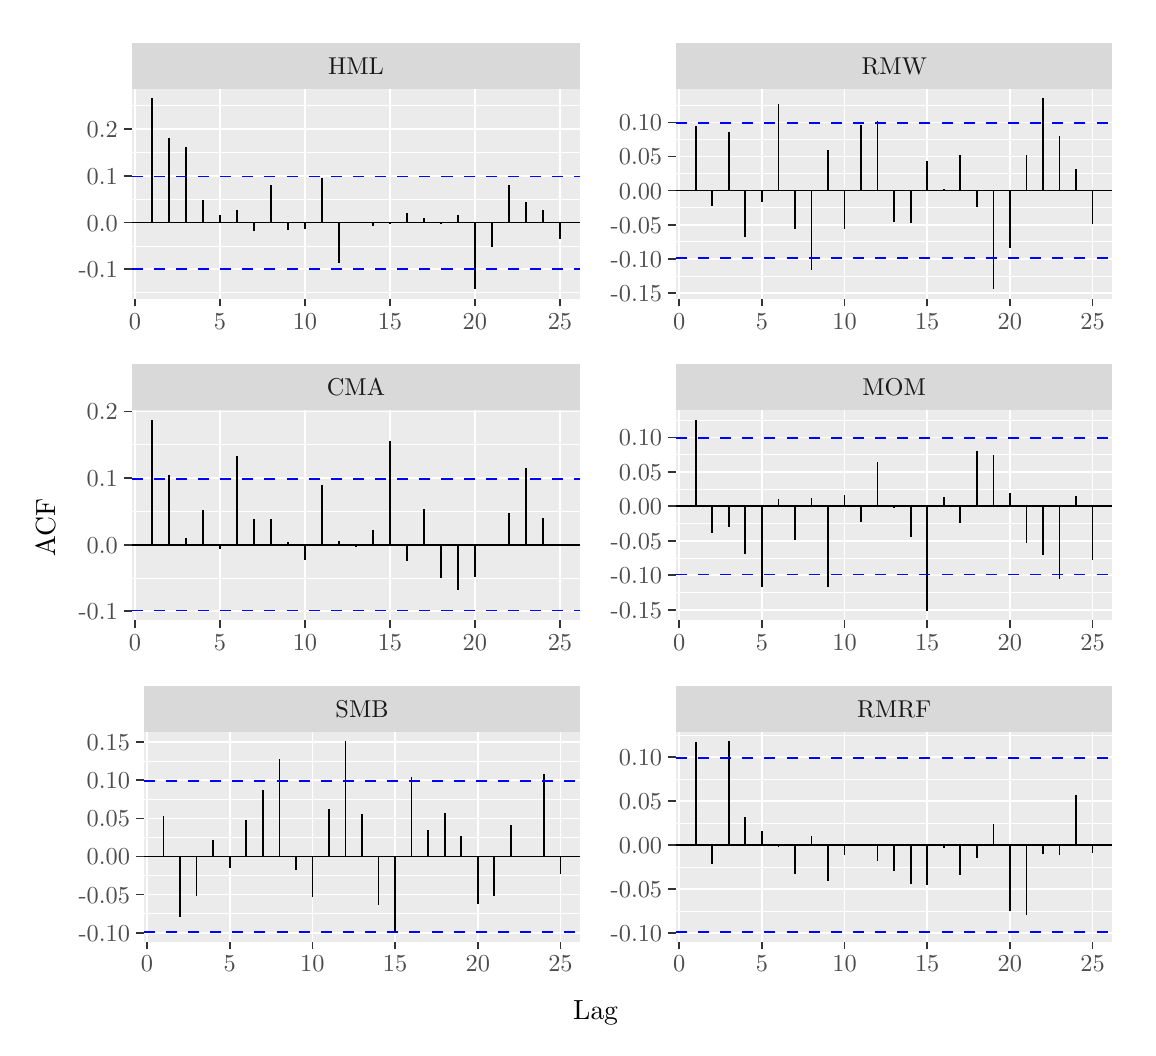
\begin{tikzpicture}[x=1pt,y=1pt]
\definecolor{fillColor}{RGB}{255,255,255}
\path[use as bounding box,fill=fillColor,fill opacity=0.00] (0,0) rectangle (397.48,361.35);
\begin{scope}
\path[clip] ( 12.91,245.20) rectangle (205.20,361.35);
\definecolor{drawColor}{RGB}{255,255,255}
\definecolor{fillColor}{RGB}{255,255,255}

\path[draw=drawColor,line width= 0.6pt,line join=round,line cap=round,fill=fillColor] ( 12.91,245.20) rectangle (205.20,361.35);
\end{scope}
\begin{scope}
\path[clip] ( 37.53,263.42) rectangle (199.70,339.28);
\definecolor{fillColor}{gray}{0.92}

\path[fill=fillColor] ( 37.53,263.42) rectangle (199.70,339.28);
\definecolor{drawColor}{RGB}{255,255,255}

\path[draw=drawColor,line width= 0.3pt,line join=round] ( 37.53,265.60) --
	(199.70,265.60);

\path[draw=drawColor,line width= 0.3pt,line join=round] ( 37.53,282.47) --
	(199.70,282.47);

\path[draw=drawColor,line width= 0.3pt,line join=round] ( 37.53,299.34) --
	(199.70,299.34);

\path[draw=drawColor,line width= 0.3pt,line join=round] ( 37.53,316.21) --
	(199.70,316.21);

\path[draw=drawColor,line width= 0.3pt,line join=round] ( 37.53,333.08) --
	(199.70,333.08);

\path[draw=drawColor,line width= 0.6pt,line join=round] ( 37.53,274.03) --
	(199.70,274.03);

\path[draw=drawColor,line width= 0.6pt,line join=round] ( 37.53,290.90) --
	(199.70,290.90);

\path[draw=drawColor,line width= 0.6pt,line join=round] ( 37.53,307.77) --
	(199.70,307.77);

\path[draw=drawColor,line width= 0.6pt,line join=round] ( 37.53,324.64) --
	(199.70,324.64);

\path[draw=drawColor,line width= 0.6pt,line join=round] ( 38.76,263.42) --
	( 38.76,339.28);

\path[draw=drawColor,line width= 0.6pt,line join=round] ( 69.48,263.42) --
	( 69.48,339.28);

\path[draw=drawColor,line width= 0.6pt,line join=round] (100.19,263.42) --
	(100.19,339.28);

\path[draw=drawColor,line width= 0.6pt,line join=round] (130.90,263.42) --
	(130.90,339.28);

\path[draw=drawColor,line width= 0.6pt,line join=round] (161.61,263.42) --
	(161.61,339.28);

\path[draw=drawColor,line width= 0.6pt,line join=round] (192.33,263.42) --
	(192.33,339.28);
\definecolor{drawColor}{RGB}{0,0,0}

\path[draw=drawColor,line width= 0.6pt,line join=round] ( 37.53,290.90) -- (199.70,290.90);

\path[draw=drawColor,line width= 0.6pt,line join=round] ( 44.91,290.90) -- ( 44.91,335.83);

\path[draw=drawColor,line width= 0.6pt,line join=round] ( 51.05,290.90) -- ( 51.05,321.49);

\path[draw=drawColor,line width= 0.6pt,line join=round] ( 57.19,290.90) -- ( 57.19,318.10);

\path[draw=drawColor,line width= 0.6pt,line join=round] ( 63.33,290.90) -- ( 63.33,299.08);

\path[draw=drawColor,line width= 0.6pt,line join=round] ( 69.48,290.90) -- ( 69.48,293.55);

\path[draw=drawColor,line width= 0.6pt,line join=round] ( 75.62,290.90) -- ( 75.62,295.48);

\path[draw=drawColor,line width= 0.6pt,line join=round] ( 81.76,290.90) -- ( 81.76,287.70);

\path[draw=drawColor,line width= 0.6pt,line join=round] ( 87.90,290.90) -- ( 87.90,304.48);

\path[draw=drawColor,line width= 0.6pt,line join=round] ( 94.05,290.90) -- ( 94.05,288.06);

\path[draw=drawColor,line width= 0.6pt,line join=round] (100.19,290.90) -- (100.19,288.60);

\path[draw=drawColor,line width= 0.6pt,line join=round] (106.33,290.90) -- (106.33,307.12);

\path[draw=drawColor,line width= 0.6pt,line join=round] (112.47,290.90) -- (112.47,276.32);

\path[draw=drawColor,line width= 0.6pt,line join=round] (118.62,290.90) -- (118.62,291.24);

\path[draw=drawColor,line width= 0.6pt,line join=round] (124.76,290.90) -- (124.76,289.66);

\path[draw=drawColor,line width= 0.6pt,line join=round] (130.90,290.90) -- (130.90,290.23);

\path[draw=drawColor,line width= 0.6pt,line join=round] (137.04,290.90) -- (137.04,294.36);

\path[draw=drawColor,line width= 0.6pt,line join=round] (143.19,290.90) -- (143.19,292.53);

\path[draw=drawColor,line width= 0.6pt,line join=round] (149.33,290.90) -- (149.33,290.23);

\path[draw=drawColor,line width= 0.6pt,line join=round] (155.47,290.90) -- (155.47,293.65);

\path[draw=drawColor,line width= 0.6pt,line join=round] (161.61,290.90) -- (161.61,266.87);

\path[draw=drawColor,line width= 0.6pt,line join=round] (167.76,290.90) -- (167.76,281.99);

\path[draw=drawColor,line width= 0.6pt,line join=round] (173.90,290.90) -- (173.90,304.52);

\path[draw=drawColor,line width= 0.6pt,line join=round] (180.04,290.90) -- (180.04,298.22);

\path[draw=drawColor,line width= 0.6pt,line join=round] (186.18,290.90) -- (186.18,295.41);

\path[draw=drawColor,line width= 0.6pt,line join=round] (192.33,290.90) -- (192.33,284.82);
\definecolor{drawColor}{RGB}{0,0,255}

\path[draw=drawColor,line width= 0.6pt,dash pattern=on 4pt off 4pt ,line join=round] ( 37.53,274.22) -- (199.70,274.22);

\path[draw=drawColor,line width= 0.6pt,dash pattern=on 4pt off 4pt ,line join=round] ( 37.53,307.58) -- (199.70,307.58);
\end{scope}
\begin{scope}
\path[clip] ( 37.53,339.28) rectangle (199.70,355.85);
\definecolor{fillColor}{gray}{0.85}

\path[fill=fillColor] ( 37.53,339.28) rectangle (199.70,355.85);
\definecolor{drawColor}{gray}{0.10}

\node[text=drawColor,anchor=base,inner sep=0pt, outer sep=0pt, scale=  0.88] at (118.62,344.53) {HML};
\end{scope}
\begin{scope}
\path[clip] (  0.00,  0.00) rectangle (397.48,361.35);
\definecolor{drawColor}{gray}{0.20}

\path[draw=drawColor,line width= 0.6pt,line join=round] ( 38.76,260.67) --
	( 38.76,263.42);

\path[draw=drawColor,line width= 0.6pt,line join=round] ( 69.48,260.67) --
	( 69.48,263.42);

\path[draw=drawColor,line width= 0.6pt,line join=round] (100.19,260.67) --
	(100.19,263.42);

\path[draw=drawColor,line width= 0.6pt,line join=round] (130.90,260.67) --
	(130.90,263.42);

\path[draw=drawColor,line width= 0.6pt,line join=round] (161.61,260.67) --
	(161.61,263.42);

\path[draw=drawColor,line width= 0.6pt,line join=round] (192.33,260.67) --
	(192.33,263.42);
\end{scope}
\begin{scope}
\path[clip] (  0.00,  0.00) rectangle (397.48,361.35);
\definecolor{drawColor}{gray}{0.30}

\node[text=drawColor,anchor=base,inner sep=0pt, outer sep=0pt, scale=  0.88] at ( 38.76,252.41) {0};

\node[text=drawColor,anchor=base,inner sep=0pt, outer sep=0pt, scale=  0.88] at ( 69.48,252.41) {5};

\node[text=drawColor,anchor=base,inner sep=0pt, outer sep=0pt, scale=  0.88] at (100.19,252.41) {10};

\node[text=drawColor,anchor=base,inner sep=0pt, outer sep=0pt, scale=  0.88] at (130.90,252.41) {15};

\node[text=drawColor,anchor=base,inner sep=0pt, outer sep=0pt, scale=  0.88] at (161.61,252.41) {20};

\node[text=drawColor,anchor=base,inner sep=0pt, outer sep=0pt, scale=  0.88] at (192.33,252.41) {25};
\end{scope}
\begin{scope}
\path[clip] (  0.00,  0.00) rectangle (397.48,361.35);
\definecolor{drawColor}{gray}{0.30}

\node[text=drawColor,anchor=base east,inner sep=0pt, outer sep=0pt, scale=  0.88] at ( 32.58,271.00) {-0.1};

\node[text=drawColor,anchor=base east,inner sep=0pt, outer sep=0pt, scale=  0.88] at ( 32.58,287.87) {0.0};

\node[text=drawColor,anchor=base east,inner sep=0pt, outer sep=0pt, scale=  0.88] at ( 32.58,304.74) {0.1};

\node[text=drawColor,anchor=base east,inner sep=0pt, outer sep=0pt, scale=  0.88] at ( 32.58,321.61) {0.2};
\end{scope}
\begin{scope}
\path[clip] (  0.00,  0.00) rectangle (397.48,361.35);
\definecolor{drawColor}{gray}{0.20}

\path[draw=drawColor,line width= 0.6pt,line join=round] ( 34.78,274.03) --
	( 37.53,274.03);

\path[draw=drawColor,line width= 0.6pt,line join=round] ( 34.78,290.90) --
	( 37.53,290.90);

\path[draw=drawColor,line width= 0.6pt,line join=round] ( 34.78,307.77) --
	( 37.53,307.77);

\path[draw=drawColor,line width= 0.6pt,line join=round] ( 34.78,324.64) --
	( 37.53,324.64);
\end{scope}
\begin{scope}
\path[clip] (205.20,245.20) rectangle (397.48,361.35);
\definecolor{drawColor}{RGB}{255,255,255}
\definecolor{fillColor}{RGB}{255,255,255}

\path[draw=drawColor,line width= 0.6pt,line join=round,line cap=round,fill=fillColor] (205.20,245.20) rectangle (397.48,361.35);
\end{scope}
\begin{scope}
\path[clip] (234.22,263.42) rectangle (391.98,339.28);
\definecolor{fillColor}{gray}{0.92}

\path[fill=fillColor] (234.22,263.42) rectangle (391.98,339.28);
\definecolor{drawColor}{RGB}{255,255,255}

\path[draw=drawColor,line width= 0.3pt,line join=round] (234.22,271.64) --
	(391.98,271.64);

\path[draw=drawColor,line width= 0.3pt,line join=round] (234.22,283.97) --
	(391.98,283.97);

\path[draw=drawColor,line width= 0.3pt,line join=round] (234.22,296.29) --
	(391.98,296.29);

\path[draw=drawColor,line width= 0.3pt,line join=round] (234.22,308.62) --
	(391.98,308.62);

\path[draw=drawColor,line width= 0.3pt,line join=round] (234.22,320.94) --
	(391.98,320.94);

\path[draw=drawColor,line width= 0.3pt,line join=round] (234.22,333.27) --
	(391.98,333.27);

\path[draw=drawColor,line width= 0.6pt,line join=round] (234.22,265.48) --
	(391.98,265.48);

\path[draw=drawColor,line width= 0.6pt,line join=round] (234.22,277.80) --
	(391.98,277.80);

\path[draw=drawColor,line width= 0.6pt,line join=round] (234.22,290.13) --
	(391.98,290.13);

\path[draw=drawColor,line width= 0.6pt,line join=round] (234.22,302.46) --
	(391.98,302.46);

\path[draw=drawColor,line width= 0.6pt,line join=round] (234.22,314.78) --
	(391.98,314.78);

\path[draw=drawColor,line width= 0.6pt,line join=round] (234.22,327.11) --
	(391.98,327.11);

\path[draw=drawColor,line width= 0.6pt,line join=round] (235.42,263.42) --
	(235.42,339.28);

\path[draw=drawColor,line width= 0.6pt,line join=round] (265.30,263.42) --
	(265.30,339.28);

\path[draw=drawColor,line width= 0.6pt,line join=round] (295.18,263.42) --
	(295.18,339.28);

\path[draw=drawColor,line width= 0.6pt,line join=round] (325.05,263.42) --
	(325.05,339.28);

\path[draw=drawColor,line width= 0.6pt,line join=round] (354.93,263.42) --
	(354.93,339.28);

\path[draw=drawColor,line width= 0.6pt,line join=round] (384.81,263.42) --
	(384.81,339.28);
\definecolor{drawColor}{RGB}{0,0,0}

\path[draw=drawColor,line width= 0.6pt,line join=round] (234.22,302.46) -- (391.98,302.46);

\path[draw=drawColor,line width= 0.6pt,line join=round] (241.39,302.46) -- (241.39,325.99);

\path[draw=drawColor,line width= 0.6pt,line join=round] (247.37,302.46) -- (247.37,296.86);

\path[draw=drawColor,line width= 0.6pt,line join=round] (253.34,302.46) -- (253.34,323.74);

\path[draw=drawColor,line width= 0.6pt,line join=round] (259.32,302.46) -- (259.32,285.78);

\path[draw=drawColor,line width= 0.6pt,line join=round] (265.30,302.46) -- (265.30,298.36);

\path[draw=drawColor,line width= 0.6pt,line join=round] (271.27,302.46) -- (271.27,333.59);

\path[draw=drawColor,line width= 0.6pt,line join=round] (277.25,302.46) -- (277.25,288.76);

\path[draw=drawColor,line width= 0.6pt,line join=round] (283.22,302.46) -- (283.22,273.76);

\path[draw=drawColor,line width= 0.6pt,line join=round] (289.20,302.46) -- (289.20,317.10);

\path[draw=drawColor,line width= 0.6pt,line join=round] (295.18,302.46) -- (295.18,288.64);

\path[draw=drawColor,line width= 0.6pt,line join=round] (301.15,302.46) -- (301.15,326.00);

\path[draw=drawColor,line width= 0.6pt,line join=round] (307.13,302.46) -- (307.13,327.77);

\path[draw=drawColor,line width= 0.6pt,line join=round] (313.10,302.46) -- (313.10,291.11);

\path[draw=drawColor,line width= 0.6pt,line join=round] (319.08,302.46) -- (319.08,290.89);

\path[draw=drawColor,line width= 0.6pt,line join=round] (325.05,302.46) -- (325.05,313.15);

\path[draw=drawColor,line width= 0.6pt,line join=round] (331.03,302.46) -- (331.03,303.15);

\path[draw=drawColor,line width= 0.6pt,line join=round] (337.01,302.46) -- (337.01,315.32);

\path[draw=drawColor,line width= 0.6pt,line join=round] (342.98,302.46) -- (342.98,296.53);

\path[draw=drawColor,line width= 0.6pt,line join=round] (348.96,302.46) -- (348.96,266.87);

\path[draw=drawColor,line width= 0.6pt,line join=round] (354.93,302.46) -- (354.93,281.58);

\path[draw=drawColor,line width= 0.6pt,line join=round] (360.91,302.46) -- (360.91,315.46);

\path[draw=drawColor,line width= 0.6pt,line join=round] (366.89,302.46) -- (366.89,335.83);

\path[draw=drawColor,line width= 0.6pt,line join=round] (372.86,302.46) -- (372.86,322.16);

\path[draw=drawColor,line width= 0.6pt,line join=round] (378.84,302.46) -- (378.84,310.37);

\path[draw=drawColor,line width= 0.6pt,line join=round] (384.81,302.46) -- (384.81,290.56);
\definecolor{drawColor}{RGB}{0,0,255}

\path[draw=drawColor,line width= 0.6pt,dash pattern=on 4pt off 4pt ,line join=round] (234.22,278.08) -- (391.98,278.08);

\path[draw=drawColor,line width= 0.6pt,dash pattern=on 4pt off 4pt ,line join=round] (234.22,326.83) -- (391.98,326.83);
\end{scope}
\begin{scope}
\path[clip] (234.22,339.28) rectangle (391.98,355.85);
\definecolor{fillColor}{gray}{0.85}

\path[fill=fillColor] (234.22,339.28) rectangle (391.98,355.85);
\definecolor{drawColor}{gray}{0.10}

\node[text=drawColor,anchor=base,inner sep=0pt, outer sep=0pt, scale=  0.88] at (313.10,344.53) {RMW};
\end{scope}
\begin{scope}
\path[clip] (  0.00,  0.00) rectangle (397.48,361.35);
\definecolor{drawColor}{gray}{0.20}

\path[draw=drawColor,line width= 0.6pt,line join=round] (235.42,260.67) --
	(235.42,263.42);

\path[draw=drawColor,line width= 0.6pt,line join=round] (265.30,260.67) --
	(265.30,263.42);

\path[draw=drawColor,line width= 0.6pt,line join=round] (295.18,260.67) --
	(295.18,263.42);

\path[draw=drawColor,line width= 0.6pt,line join=round] (325.05,260.67) --
	(325.05,263.42);

\path[draw=drawColor,line width= 0.6pt,line join=round] (354.93,260.67) --
	(354.93,263.42);

\path[draw=drawColor,line width= 0.6pt,line join=round] (384.81,260.67) --
	(384.81,263.42);
\end{scope}
\begin{scope}
\path[clip] (  0.00,  0.00) rectangle (397.48,361.35);
\definecolor{drawColor}{gray}{0.30}

\node[text=drawColor,anchor=base,inner sep=0pt, outer sep=0pt, scale=  0.88] at (235.42,252.41) {0};

\node[text=drawColor,anchor=base,inner sep=0pt, outer sep=0pt, scale=  0.88] at (265.30,252.41) {5};

\node[text=drawColor,anchor=base,inner sep=0pt, outer sep=0pt, scale=  0.88] at (295.18,252.41) {10};

\node[text=drawColor,anchor=base,inner sep=0pt, outer sep=0pt, scale=  0.88] at (325.05,252.41) {15};

\node[text=drawColor,anchor=base,inner sep=0pt, outer sep=0pt, scale=  0.88] at (354.93,252.41) {20};

\node[text=drawColor,anchor=base,inner sep=0pt, outer sep=0pt, scale=  0.88] at (384.81,252.41) {25};
\end{scope}
\begin{scope}
\path[clip] (  0.00,  0.00) rectangle (397.48,361.35);
\definecolor{drawColor}{gray}{0.30}

\node[text=drawColor,anchor=base east,inner sep=0pt, outer sep=0pt, scale=  0.88] at (229.27,262.45) {-0.15};

\node[text=drawColor,anchor=base east,inner sep=0pt, outer sep=0pt, scale=  0.88] at (229.27,274.77) {-0.10};

\node[text=drawColor,anchor=base east,inner sep=0pt, outer sep=0pt, scale=  0.88] at (229.27,287.10) {-0.05};

\node[text=drawColor,anchor=base east,inner sep=0pt, outer sep=0pt, scale=  0.88] at (229.27,299.42) {0.00};

\node[text=drawColor,anchor=base east,inner sep=0pt, outer sep=0pt, scale=  0.88] at (229.27,311.75) {0.05};

\node[text=drawColor,anchor=base east,inner sep=0pt, outer sep=0pt, scale=  0.88] at (229.27,324.08) {0.10};
\end{scope}
\begin{scope}
\path[clip] (  0.00,  0.00) rectangle (397.48,361.35);
\definecolor{drawColor}{gray}{0.20}

\path[draw=drawColor,line width= 0.6pt,line join=round] (231.47,265.48) --
	(234.22,265.48);

\path[draw=drawColor,line width= 0.6pt,line join=round] (231.47,277.80) --
	(234.22,277.80);

\path[draw=drawColor,line width= 0.6pt,line join=round] (231.47,290.13) --
	(234.22,290.13);

\path[draw=drawColor,line width= 0.6pt,line join=round] (231.47,302.46) --
	(234.22,302.46);

\path[draw=drawColor,line width= 0.6pt,line join=round] (231.47,314.78) --
	(234.22,314.78);

\path[draw=drawColor,line width= 0.6pt,line join=round] (231.47,327.11) --
	(234.22,327.11);
\end{scope}
\begin{scope}
\path[clip] ( 12.91,129.06) rectangle (205.20,245.20);
\definecolor{drawColor}{RGB}{255,255,255}
\definecolor{fillColor}{RGB}{255,255,255}

\path[draw=drawColor,line width= 0.6pt,line join=round,line cap=round,fill=fillColor] ( 12.91,129.06) rectangle (205.20,245.20);
\end{scope}
\begin{scope}
\path[clip] ( 37.53,147.28) rectangle (199.70,223.13);
\definecolor{fillColor}{gray}{0.92}

\path[fill=fillColor] ( 37.53,147.28) rectangle (199.70,223.13);
\definecolor{drawColor}{RGB}{255,255,255}

\path[draw=drawColor,line width= 0.3pt,line join=round] ( 37.53,162.49) --
	(199.70,162.49);

\path[draw=drawColor,line width= 0.3pt,line join=round] ( 37.53,186.57) --
	(199.70,186.57);

\path[draw=drawColor,line width= 0.3pt,line join=round] ( 37.53,210.65) --
	(199.70,210.65);

\path[draw=drawColor,line width= 0.6pt,line join=round] ( 37.53,150.45) --
	(199.70,150.45);

\path[draw=drawColor,line width= 0.6pt,line join=round] ( 37.53,174.53) --
	(199.70,174.53);

\path[draw=drawColor,line width= 0.6pt,line join=round] ( 37.53,198.61) --
	(199.70,198.61);

\path[draw=drawColor,line width= 0.6pt,line join=round] ( 37.53,222.68) --
	(199.70,222.68);

\path[draw=drawColor,line width= 0.6pt,line join=round] ( 38.76,147.28) --
	( 38.76,223.13);

\path[draw=drawColor,line width= 0.6pt,line join=round] ( 69.48,147.28) --
	( 69.48,223.13);

\path[draw=drawColor,line width= 0.6pt,line join=round] (100.19,147.28) --
	(100.19,223.13);

\path[draw=drawColor,line width= 0.6pt,line join=round] (130.90,147.28) --
	(130.90,223.13);

\path[draw=drawColor,line width= 0.6pt,line join=round] (161.61,147.28) --
	(161.61,223.13);

\path[draw=drawColor,line width= 0.6pt,line join=round] (192.33,147.28) --
	(192.33,223.13);
\definecolor{drawColor}{RGB}{0,0,0}

\path[draw=drawColor,line width= 0.6pt,line join=round] ( 37.53,174.53) -- (199.70,174.53);

\path[draw=drawColor,line width= 0.6pt,line join=round] ( 44.91,174.53) -- ( 44.91,219.68);

\path[draw=drawColor,line width= 0.6pt,line join=round] ( 51.05,174.53) -- ( 51.05,199.77);

\path[draw=drawColor,line width= 0.6pt,line join=round] ( 57.19,174.53) -- ( 57.19,177.12);

\path[draw=drawColor,line width= 0.6pt,line join=round] ( 63.33,174.53) -- ( 63.33,187.08);

\path[draw=drawColor,line width= 0.6pt,line join=round] ( 69.48,174.53) -- ( 69.48,173.10);

\path[draw=drawColor,line width= 0.6pt,line join=round] ( 75.62,174.53) -- ( 75.62,206.74);

\path[draw=drawColor,line width= 0.6pt,line join=round] ( 81.76,174.53) -- ( 81.76,183.67);

\path[draw=drawColor,line width= 0.6pt,line join=round] ( 87.90,174.53) -- ( 87.90,183.64);

\path[draw=drawColor,line width= 0.6pt,line join=round] ( 94.05,174.53) -- ( 94.05,175.46);

\path[draw=drawColor,line width= 0.6pt,line join=round] (100.19,174.53) -- (100.19,168.87);

\path[draw=drawColor,line width= 0.6pt,line join=round] (106.33,174.53) -- (106.33,196.01);

\path[draw=drawColor,line width= 0.6pt,line join=round] (112.47,174.53) -- (112.47,175.73);

\path[draw=drawColor,line width= 0.6pt,line join=round] (118.62,174.53) -- (118.62,173.69);

\path[draw=drawColor,line width= 0.6pt,line join=round] (124.76,174.53) -- (124.76,179.90);

\path[draw=drawColor,line width= 0.6pt,line join=round] (130.90,174.53) -- (130.90,211.86);

\path[draw=drawColor,line width= 0.6pt,line join=round] (137.04,174.53) -- (137.04,168.52);

\path[draw=drawColor,line width= 0.6pt,line join=round] (143.19,174.53) -- (143.19,187.31);

\path[draw=drawColor,line width= 0.6pt,line join=round] (149.33,174.53) -- (149.33,162.62);

\path[draw=drawColor,line width= 0.6pt,line join=round] (155.47,174.53) -- (155.47,158.12);

\path[draw=drawColor,line width= 0.6pt,line join=round] (161.61,174.53) -- (161.61,162.93);

\path[draw=drawColor,line width= 0.6pt,line join=round] (167.76,174.53) -- (167.76,174.25);

\path[draw=drawColor,line width= 0.6pt,line join=round] (173.90,174.53) -- (173.90,185.98);

\path[draw=drawColor,line width= 0.6pt,line join=round] (180.04,174.53) -- (180.04,202.32);

\path[draw=drawColor,line width= 0.6pt,line join=round] (186.18,174.53) -- (186.18,184.23);

\path[draw=drawColor,line width= 0.6pt,line join=round] (192.33,174.53) -- (192.33,174.24);
\definecolor{drawColor}{RGB}{0,0,255}

\path[draw=drawColor,line width= 0.6pt,dash pattern=on 4pt off 4pt ,line join=round] ( 37.53,150.73) -- (199.70,150.73);

\path[draw=drawColor,line width= 0.6pt,dash pattern=on 4pt off 4pt ,line join=round] ( 37.53,198.33) -- (199.70,198.33);
\end{scope}
\begin{scope}
\path[clip] ( 37.53,223.13) rectangle (199.70,239.70);
\definecolor{fillColor}{gray}{0.85}

\path[fill=fillColor] ( 37.53,223.13) rectangle (199.70,239.70);
\definecolor{drawColor}{gray}{0.10}

\node[text=drawColor,anchor=base,inner sep=0pt, outer sep=0pt, scale=  0.88] at (118.62,228.39) {CMA};
\end{scope}
\begin{scope}
\path[clip] (  0.00,  0.00) rectangle (397.48,361.35);
\definecolor{drawColor}{gray}{0.20}

\path[draw=drawColor,line width= 0.6pt,line join=round] ( 38.76,144.53) --
	( 38.76,147.28);

\path[draw=drawColor,line width= 0.6pt,line join=round] ( 69.48,144.53) --
	( 69.48,147.28);

\path[draw=drawColor,line width= 0.6pt,line join=round] (100.19,144.53) --
	(100.19,147.28);

\path[draw=drawColor,line width= 0.6pt,line join=round] (130.90,144.53) --
	(130.90,147.28);

\path[draw=drawColor,line width= 0.6pt,line join=round] (161.61,144.53) --
	(161.61,147.28);

\path[draw=drawColor,line width= 0.6pt,line join=round] (192.33,144.53) --
	(192.33,147.28);
\end{scope}
\begin{scope}
\path[clip] (  0.00,  0.00) rectangle (397.48,361.35);
\definecolor{drawColor}{gray}{0.30}

\node[text=drawColor,anchor=base,inner sep=0pt, outer sep=0pt, scale=  0.88] at ( 38.76,136.27) {0};

\node[text=drawColor,anchor=base,inner sep=0pt, outer sep=0pt, scale=  0.88] at ( 69.48,136.27) {5};

\node[text=drawColor,anchor=base,inner sep=0pt, outer sep=0pt, scale=  0.88] at (100.19,136.27) {10};

\node[text=drawColor,anchor=base,inner sep=0pt, outer sep=0pt, scale=  0.88] at (130.90,136.27) {15};

\node[text=drawColor,anchor=base,inner sep=0pt, outer sep=0pt, scale=  0.88] at (161.61,136.27) {20};

\node[text=drawColor,anchor=base,inner sep=0pt, outer sep=0pt, scale=  0.88] at (192.33,136.27) {25};
\end{scope}
\begin{scope}
\path[clip] (  0.00,  0.00) rectangle (397.48,361.35);
\definecolor{drawColor}{gray}{0.30}

\node[text=drawColor,anchor=base east,inner sep=0pt, outer sep=0pt, scale=  0.88] at ( 32.58,147.42) {-0.1};

\node[text=drawColor,anchor=base east,inner sep=0pt, outer sep=0pt, scale=  0.88] at ( 32.58,171.50) {0.0};

\node[text=drawColor,anchor=base east,inner sep=0pt, outer sep=0pt, scale=  0.88] at ( 32.58,195.58) {0.1};

\node[text=drawColor,anchor=base east,inner sep=0pt, outer sep=0pt, scale=  0.88] at ( 32.58,219.65) {0.2};
\end{scope}
\begin{scope}
\path[clip] (  0.00,  0.00) rectangle (397.48,361.35);
\definecolor{drawColor}{gray}{0.20}

\path[draw=drawColor,line width= 0.6pt,line join=round] ( 34.78,150.45) --
	( 37.53,150.45);

\path[draw=drawColor,line width= 0.6pt,line join=round] ( 34.78,174.53) --
	( 37.53,174.53);

\path[draw=drawColor,line width= 0.6pt,line join=round] ( 34.78,198.61) --
	( 37.53,198.61);

\path[draw=drawColor,line width= 0.6pt,line join=round] ( 34.78,222.68) --
	( 37.53,222.68);
\end{scope}
\begin{scope}
\path[clip] (205.20,129.06) rectangle (397.48,245.20);
\definecolor{drawColor}{RGB}{255,255,255}
\definecolor{fillColor}{RGB}{255,255,255}

\path[draw=drawColor,line width= 0.6pt,line join=round,line cap=round,fill=fillColor] (205.20,129.06) rectangle (397.48,245.20);
\end{scope}
\begin{scope}
\path[clip] (234.22,147.28) rectangle (391.98,223.13);
\definecolor{fillColor}{gray}{0.92}

\path[fill=fillColor] (234.22,147.28) rectangle (391.98,223.13);
\definecolor{drawColor}{RGB}{255,255,255}

\path[draw=drawColor,line width= 0.3pt,line join=round] (234.22,157.27) --
	(391.98,157.27);

\path[draw=drawColor,line width= 0.3pt,line join=round] (234.22,169.72) --
	(391.98,169.72);

\path[draw=drawColor,line width= 0.3pt,line join=round] (234.22,182.17) --
	(391.98,182.17);

\path[draw=drawColor,line width= 0.3pt,line join=round] (234.22,194.62) --
	(391.98,194.62);

\path[draw=drawColor,line width= 0.3pt,line join=round] (234.22,207.07) --
	(391.98,207.07);

\path[draw=drawColor,line width= 0.3pt,line join=round] (234.22,219.52) --
	(391.98,219.52);

\path[draw=drawColor,line width= 0.6pt,line join=round] (234.22,151.04) --
	(391.98,151.04);

\path[draw=drawColor,line width= 0.6pt,line join=round] (234.22,163.49) --
	(391.98,163.49);

\path[draw=drawColor,line width= 0.6pt,line join=round] (234.22,175.94) --
	(391.98,175.94);

\path[draw=drawColor,line width= 0.6pt,line join=round] (234.22,188.39) --
	(391.98,188.39);

\path[draw=drawColor,line width= 0.6pt,line join=round] (234.22,200.84) --
	(391.98,200.84);

\path[draw=drawColor,line width= 0.6pt,line join=round] (234.22,213.29) --
	(391.98,213.29);

\path[draw=drawColor,line width= 0.6pt,line join=round] (235.42,147.28) --
	(235.42,223.13);

\path[draw=drawColor,line width= 0.6pt,line join=round] (265.30,147.28) --
	(265.30,223.13);

\path[draw=drawColor,line width= 0.6pt,line join=round] (295.18,147.28) --
	(295.18,223.13);

\path[draw=drawColor,line width= 0.6pt,line join=round] (325.05,147.28) --
	(325.05,223.13);

\path[draw=drawColor,line width= 0.6pt,line join=round] (354.93,147.28) --
	(354.93,223.13);

\path[draw=drawColor,line width= 0.6pt,line join=round] (384.81,147.28) --
	(384.81,223.13);
\definecolor{drawColor}{RGB}{0,0,0}

\path[draw=drawColor,line width= 0.6pt,line join=round] (234.22,188.39) -- (391.98,188.39);

\path[draw=drawColor,line width= 0.6pt,line join=round] (241.39,188.39) -- (241.39,219.68);

\path[draw=drawColor,line width= 0.6pt,line join=round] (247.37,188.39) -- (247.37,178.60);

\path[draw=drawColor,line width= 0.6pt,line join=round] (253.34,188.39) -- (253.34,180.99);

\path[draw=drawColor,line width= 0.6pt,line join=round] (259.32,188.39) -- (259.32,171.13);

\path[draw=drawColor,line width= 0.6pt,line join=round] (265.30,188.39) -- (265.30,159.34);

\path[draw=drawColor,line width= 0.6pt,line join=round] (271.27,188.39) -- (271.27,190.92);

\path[draw=drawColor,line width= 0.6pt,line join=round] (277.25,188.39) -- (277.25,176.08);

\path[draw=drawColor,line width= 0.6pt,line join=round] (283.22,188.39) -- (283.22,191.49);

\path[draw=drawColor,line width= 0.6pt,line join=round] (289.20,188.39) -- (289.20,159.09);

\path[draw=drawColor,line width= 0.6pt,line join=round] (295.18,188.39) -- (295.18,192.59);

\path[draw=drawColor,line width= 0.6pt,line join=round] (301.15,188.39) -- (301.15,182.69);

\path[draw=drawColor,line width= 0.6pt,line join=round] (307.13,188.39) -- (307.13,204.24);

\path[draw=drawColor,line width= 0.6pt,line join=round] (313.10,188.39) -- (313.10,187.74);

\path[draw=drawColor,line width= 0.6pt,line join=round] (319.08,188.39) -- (319.08,177.20);

\path[draw=drawColor,line width= 0.6pt,line join=round] (325.05,188.39) -- (325.05,150.73);

\path[draw=drawColor,line width= 0.6pt,line join=round] (331.03,188.39) -- (331.03,191.77);

\path[draw=drawColor,line width= 0.6pt,line join=round] (337.01,188.39) -- (337.01,182.29);

\path[draw=drawColor,line width= 0.6pt,line join=round] (342.98,188.39) -- (342.98,208.47);

\path[draw=drawColor,line width= 0.6pt,line join=round] (348.96,188.39) -- (348.96,206.82);

\path[draw=drawColor,line width= 0.6pt,line join=round] (354.93,188.39) -- (354.93,193.24);

\path[draw=drawColor,line width= 0.6pt,line join=round] (360.91,188.39) -- (360.91,175.18);

\path[draw=drawColor,line width= 0.6pt,line join=round] (366.89,188.39) -- (366.89,170.87);

\path[draw=drawColor,line width= 0.6pt,line join=round] (372.86,188.39) -- (372.86,162.02);

\path[draw=drawColor,line width= 0.6pt,line join=round] (378.84,188.39) -- (378.84,192.15);

\path[draw=drawColor,line width= 0.6pt,line join=round] (384.81,188.39) -- (384.81,168.93);
\definecolor{drawColor}{RGB}{0,0,255}

\path[draw=drawColor,line width= 0.6pt,dash pattern=on 4pt off 4pt ,line join=round] (234.22,163.77) -- (391.98,163.77);

\path[draw=drawColor,line width= 0.6pt,dash pattern=on 4pt off 4pt ,line join=round] (234.22,213.01) -- (391.98,213.01);
\end{scope}
\begin{scope}
\path[clip] (234.22,223.13) rectangle (391.98,239.70);
\definecolor{fillColor}{gray}{0.85}

\path[fill=fillColor] (234.22,223.13) rectangle (391.98,239.70);
\definecolor{drawColor}{gray}{0.10}

\node[text=drawColor,anchor=base,inner sep=0pt, outer sep=0pt, scale=  0.88] at (313.10,228.39) {MOM};
\end{scope}
\begin{scope}
\path[clip] (  0.00,  0.00) rectangle (397.48,361.35);
\definecolor{drawColor}{gray}{0.20}

\path[draw=drawColor,line width= 0.6pt,line join=round] (235.42,144.53) --
	(235.42,147.28);

\path[draw=drawColor,line width= 0.6pt,line join=round] (265.30,144.53) --
	(265.30,147.28);

\path[draw=drawColor,line width= 0.6pt,line join=round] (295.18,144.53) --
	(295.18,147.28);

\path[draw=drawColor,line width= 0.6pt,line join=round] (325.05,144.53) --
	(325.05,147.28);

\path[draw=drawColor,line width= 0.6pt,line join=round] (354.93,144.53) --
	(354.93,147.28);

\path[draw=drawColor,line width= 0.6pt,line join=round] (384.81,144.53) --
	(384.81,147.28);
\end{scope}
\begin{scope}
\path[clip] (  0.00,  0.00) rectangle (397.48,361.35);
\definecolor{drawColor}{gray}{0.30}

\node[text=drawColor,anchor=base,inner sep=0pt, outer sep=0pt, scale=  0.88] at (235.42,136.27) {0};

\node[text=drawColor,anchor=base,inner sep=0pt, outer sep=0pt, scale=  0.88] at (265.30,136.27) {5};

\node[text=drawColor,anchor=base,inner sep=0pt, outer sep=0pt, scale=  0.88] at (295.18,136.27) {10};

\node[text=drawColor,anchor=base,inner sep=0pt, outer sep=0pt, scale=  0.88] at (325.05,136.27) {15};

\node[text=drawColor,anchor=base,inner sep=0pt, outer sep=0pt, scale=  0.88] at (354.93,136.27) {20};

\node[text=drawColor,anchor=base,inner sep=0pt, outer sep=0pt, scale=  0.88] at (384.81,136.27) {25};
\end{scope}
\begin{scope}
\path[clip] (  0.00,  0.00) rectangle (397.48,361.35);
\definecolor{drawColor}{gray}{0.30}

\node[text=drawColor,anchor=base east,inner sep=0pt, outer sep=0pt, scale=  0.88] at (229.27,148.01) {-0.15};

\node[text=drawColor,anchor=base east,inner sep=0pt, outer sep=0pt, scale=  0.88] at (229.27,160.46) {-0.10};

\node[text=drawColor,anchor=base east,inner sep=0pt, outer sep=0pt, scale=  0.88] at (229.27,172.91) {-0.05};

\node[text=drawColor,anchor=base east,inner sep=0pt, outer sep=0pt, scale=  0.88] at (229.27,185.36) {0.00};

\node[text=drawColor,anchor=base east,inner sep=0pt, outer sep=0pt, scale=  0.88] at (229.27,197.81) {0.05};

\node[text=drawColor,anchor=base east,inner sep=0pt, outer sep=0pt, scale=  0.88] at (229.27,210.26) {0.10};
\end{scope}
\begin{scope}
\path[clip] (  0.00,  0.00) rectangle (397.48,361.35);
\definecolor{drawColor}{gray}{0.20}

\path[draw=drawColor,line width= 0.6pt,line join=round] (231.47,151.04) --
	(234.22,151.04);

\path[draw=drawColor,line width= 0.6pt,line join=round] (231.47,163.49) --
	(234.22,163.49);

\path[draw=drawColor,line width= 0.6pt,line join=round] (231.47,175.94) --
	(234.22,175.94);

\path[draw=drawColor,line width= 0.6pt,line join=round] (231.47,188.39) --
	(234.22,188.39);

\path[draw=drawColor,line width= 0.6pt,line join=round] (231.47,200.84) --
	(234.22,200.84);

\path[draw=drawColor,line width= 0.6pt,line join=round] (231.47,213.29) --
	(234.22,213.29);
\end{scope}
\begin{scope}
\path[clip] ( 12.91, 12.91) rectangle (205.20,129.06);
\definecolor{drawColor}{RGB}{255,255,255}
\definecolor{fillColor}{RGB}{255,255,255}

\path[draw=drawColor,line width= 0.6pt,line join=round,line cap=round,fill=fillColor] ( 12.91, 12.91) rectangle (205.20,129.06);
\end{scope}
\begin{scope}
\path[clip] ( 41.93, 31.13) rectangle (199.70,106.98);
\definecolor{fillColor}{gray}{0.92}

\path[fill=fillColor] ( 41.93, 31.13) rectangle (199.70,106.98);
\definecolor{drawColor}{RGB}{255,255,255}

\path[draw=drawColor,line width= 0.3pt,line join=round] ( 41.93, 41.16) --
	(199.70, 41.16);

\path[draw=drawColor,line width= 0.3pt,line join=round] ( 41.93, 54.95) --
	(199.70, 54.95);

\path[draw=drawColor,line width= 0.3pt,line join=round] ( 41.93, 68.75) --
	(199.70, 68.75);

\path[draw=drawColor,line width= 0.3pt,line join=round] ( 41.93, 82.54) --
	(199.70, 82.54);

\path[draw=drawColor,line width= 0.3pt,line join=round] ( 41.93, 96.33) --
	(199.70, 96.33);

\path[draw=drawColor,line width= 0.6pt,line join=round] ( 41.93, 34.27) --
	(199.70, 34.27);

\path[draw=drawColor,line width= 0.6pt,line join=round] ( 41.93, 48.06) --
	(199.70, 48.06);

\path[draw=drawColor,line width= 0.6pt,line join=round] ( 41.93, 61.85) --
	(199.70, 61.85);

\path[draw=drawColor,line width= 0.6pt,line join=round] ( 41.93, 75.64) --
	(199.70, 75.64);

\path[draw=drawColor,line width= 0.6pt,line join=round] ( 41.93, 89.43) --
	(199.70, 89.43);

\path[draw=drawColor,line width= 0.6pt,line join=round] ( 41.93,103.23) --
	(199.70,103.23);

\path[draw=drawColor,line width= 0.6pt,line join=round] ( 43.13, 31.13) --
	( 43.13,106.98);

\path[draw=drawColor,line width= 0.6pt,line join=round] ( 73.01, 31.13) --
	( 73.01,106.98);

\path[draw=drawColor,line width= 0.6pt,line join=round] (102.89, 31.13) --
	(102.89,106.98);

\path[draw=drawColor,line width= 0.6pt,line join=round] (132.77, 31.13) --
	(132.77,106.98);

\path[draw=drawColor,line width= 0.6pt,line join=round] (162.65, 31.13) --
	(162.65,106.98);

\path[draw=drawColor,line width= 0.6pt,line join=round] (192.53, 31.13) --
	(192.53,106.98);
\definecolor{drawColor}{RGB}{0,0,0}

\path[draw=drawColor,line width= 0.6pt,line join=round] ( 41.93, 61.85) -- (199.70, 61.85);

\path[draw=drawColor,line width= 0.6pt,line join=round] ( 49.10, 61.85) -- ( 49.10, 76.59);

\path[draw=drawColor,line width= 0.6pt,line join=round] ( 55.08, 61.85) -- ( 55.08, 39.83);

\path[draw=drawColor,line width= 0.6pt,line join=round] ( 61.06, 61.85) -- ( 61.06, 47.43);

\path[draw=drawColor,line width= 0.6pt,line join=round] ( 67.03, 61.85) -- ( 67.03, 67.78);

\path[draw=drawColor,line width= 0.6pt,line join=round] ( 73.01, 61.85) -- ( 73.01, 57.81);

\path[draw=drawColor,line width= 0.6pt,line join=round] ( 78.98, 61.85) -- ( 78.98, 75.05);

\path[draw=drawColor,line width= 0.6pt,line join=round] ( 84.96, 61.85) -- ( 84.96, 85.87);

\path[draw=drawColor,line width= 0.6pt,line join=round] ( 90.94, 61.85) -- ( 90.94, 97.26);

\path[draw=drawColor,line width= 0.6pt,line join=round] ( 96.91, 61.85) -- ( 96.91, 56.87);

\path[draw=drawColor,line width= 0.6pt,line join=round] (102.89, 61.85) -- (102.89, 47.26);

\path[draw=drawColor,line width= 0.6pt,line join=round] (108.86, 61.85) -- (108.86, 79.07);

\path[draw=drawColor,line width= 0.6pt,line join=round] (114.84, 61.85) -- (114.84,103.54);

\path[draw=drawColor,line width= 0.6pt,line join=round] (120.82, 61.85) -- (120.82, 77.08);

\path[draw=drawColor,line width= 0.6pt,line join=round] (126.79, 61.85) -- (126.79, 44.47);

\path[draw=drawColor,line width= 0.6pt,line join=round] (132.77, 61.85) -- (132.77, 35.10);

\path[draw=drawColor,line width= 0.6pt,line join=round] (138.74, 61.85) -- (138.74, 90.68);

\path[draw=drawColor,line width= 0.6pt,line join=round] (144.72, 61.85) -- (144.72, 71.46);

\path[draw=drawColor,line width= 0.6pt,line join=round] (150.69, 61.85) -- (150.69, 77.75);

\path[draw=drawColor,line width= 0.6pt,line join=round] (156.67, 61.85) -- (156.67, 69.38);

\path[draw=drawColor,line width= 0.6pt,line join=round] (162.65, 61.85) -- (162.65, 44.72);

\path[draw=drawColor,line width= 0.6pt,line join=round] (168.62, 61.85) -- (168.62, 47.74);

\path[draw=drawColor,line width= 0.6pt,line join=round] (174.60, 61.85) -- (174.60, 73.31);

\path[draw=drawColor,line width= 0.6pt,line join=round] (180.57, 61.85) -- (180.57, 61.97);

\path[draw=drawColor,line width= 0.6pt,line join=round] (186.55, 61.85) -- (186.55, 91.61);

\path[draw=drawColor,line width= 0.6pt,line join=round] (192.53, 61.85) -- (192.53, 55.57);
\definecolor{drawColor}{RGB}{0,0,255}

\path[draw=drawColor,line width= 0.6pt,dash pattern=on 4pt off 4pt ,line join=round] ( 41.93, 34.58) -- (199.70, 34.58);

\path[draw=drawColor,line width= 0.6pt,dash pattern=on 4pt off 4pt ,line join=round] ( 41.93, 89.12) -- (199.70, 89.12);
\end{scope}
\begin{scope}
\path[clip] ( 41.93,106.98) rectangle (199.70,123.56);
\definecolor{fillColor}{gray}{0.85}

\path[fill=fillColor] ( 41.93,106.98) rectangle (199.70,123.56);
\definecolor{drawColor}{gray}{0.10}

\node[text=drawColor,anchor=base,inner sep=0pt, outer sep=0pt, scale=  0.88] at (120.82,112.24) {SMB};
\end{scope}
\begin{scope}
\path[clip] (  0.00,  0.00) rectangle (397.48,361.35);
\definecolor{drawColor}{gray}{0.20}

\path[draw=drawColor,line width= 0.6pt,line join=round] ( 43.13, 28.38) --
	( 43.13, 31.13);

\path[draw=drawColor,line width= 0.6pt,line join=round] ( 73.01, 28.38) --
	( 73.01, 31.13);

\path[draw=drawColor,line width= 0.6pt,line join=round] (102.89, 28.38) --
	(102.89, 31.13);

\path[draw=drawColor,line width= 0.6pt,line join=round] (132.77, 28.38) --
	(132.77, 31.13);

\path[draw=drawColor,line width= 0.6pt,line join=round] (162.65, 28.38) --
	(162.65, 31.13);

\path[draw=drawColor,line width= 0.6pt,line join=round] (192.53, 28.38) --
	(192.53, 31.13);
\end{scope}
\begin{scope}
\path[clip] (  0.00,  0.00) rectangle (397.48,361.35);
\definecolor{drawColor}{gray}{0.30}

\node[text=drawColor,anchor=base,inner sep=0pt, outer sep=0pt, scale=  0.88] at ( 43.13, 20.12) {0};

\node[text=drawColor,anchor=base,inner sep=0pt, outer sep=0pt, scale=  0.88] at ( 73.01, 20.12) {5};

\node[text=drawColor,anchor=base,inner sep=0pt, outer sep=0pt, scale=  0.88] at (102.89, 20.12) {10};

\node[text=drawColor,anchor=base,inner sep=0pt, outer sep=0pt, scale=  0.88] at (132.77, 20.12) {15};

\node[text=drawColor,anchor=base,inner sep=0pt, outer sep=0pt, scale=  0.88] at (162.65, 20.12) {20};

\node[text=drawColor,anchor=base,inner sep=0pt, outer sep=0pt, scale=  0.88] at (192.53, 20.12) {25};
\end{scope}
\begin{scope}
\path[clip] (  0.00,  0.00) rectangle (397.48,361.35);
\definecolor{drawColor}{gray}{0.30}

\node[text=drawColor,anchor=base east,inner sep=0pt, outer sep=0pt, scale=  0.88] at ( 36.98, 31.24) {-0.10};

\node[text=drawColor,anchor=base east,inner sep=0pt, outer sep=0pt, scale=  0.88] at ( 36.98, 45.03) {-0.05};

\node[text=drawColor,anchor=base east,inner sep=0pt, outer sep=0pt, scale=  0.88] at ( 36.98, 58.82) {0.00};

\node[text=drawColor,anchor=base east,inner sep=0pt, outer sep=0pt, scale=  0.88] at ( 36.98, 72.61) {0.05};

\node[text=drawColor,anchor=base east,inner sep=0pt, outer sep=0pt, scale=  0.88] at ( 36.98, 86.40) {0.10};

\node[text=drawColor,anchor=base east,inner sep=0pt, outer sep=0pt, scale=  0.88] at ( 36.98,100.20) {0.15};
\end{scope}
\begin{scope}
\path[clip] (  0.00,  0.00) rectangle (397.48,361.35);
\definecolor{drawColor}{gray}{0.20}

\path[draw=drawColor,line width= 0.6pt,line join=round] ( 39.18, 34.27) --
	( 41.93, 34.27);

\path[draw=drawColor,line width= 0.6pt,line join=round] ( 39.18, 48.06) --
	( 41.93, 48.06);

\path[draw=drawColor,line width= 0.6pt,line join=round] ( 39.18, 61.85) --
	( 41.93, 61.85);

\path[draw=drawColor,line width= 0.6pt,line join=round] ( 39.18, 75.64) --
	( 41.93, 75.64);

\path[draw=drawColor,line width= 0.6pt,line join=round] ( 39.18, 89.43) --
	( 41.93, 89.43);

\path[draw=drawColor,line width= 0.6pt,line join=round] ( 39.18,103.23) --
	( 41.93,103.23);
\end{scope}
\begin{scope}
\path[clip] (205.20, 12.91) rectangle (397.48,129.06);
\definecolor{drawColor}{RGB}{255,255,255}
\definecolor{fillColor}{RGB}{255,255,255}

\path[draw=drawColor,line width= 0.6pt,line join=round,line cap=round,fill=fillColor] (205.20, 12.91) rectangle (397.48,129.06);
\end{scope}
\begin{scope}
\path[clip] (234.22, 31.13) rectangle (391.98,106.98);
\definecolor{fillColor}{gray}{0.92}

\path[fill=fillColor] (234.22, 31.13) rectangle (391.98,106.98);
\definecolor{drawColor}{RGB}{255,255,255}

\path[draw=drawColor,line width= 0.3pt,line join=round] (234.22, 42.16) --
	(391.98, 42.16);

\path[draw=drawColor,line width= 0.3pt,line join=round] (234.22, 58.05) --
	(391.98, 58.05);

\path[draw=drawColor,line width= 0.3pt,line join=round] (234.22, 73.95) --
	(391.98, 73.95);

\path[draw=drawColor,line width= 0.3pt,line join=round] (234.22, 89.84) --
	(391.98, 89.84);

\path[draw=drawColor,line width= 0.3pt,line join=round] (234.22,105.73) --
	(391.98,105.73);

\path[draw=drawColor,line width= 0.6pt,line join=round] (234.22, 34.22) --
	(391.98, 34.22);

\path[draw=drawColor,line width= 0.6pt,line join=round] (234.22, 50.11) --
	(391.98, 50.11);

\path[draw=drawColor,line width= 0.6pt,line join=round] (234.22, 66.00) --
	(391.98, 66.00);

\path[draw=drawColor,line width= 0.6pt,line join=round] (234.22, 81.89) --
	(391.98, 81.89);

\path[draw=drawColor,line width= 0.6pt,line join=round] (234.22, 97.78) --
	(391.98, 97.78);

\path[draw=drawColor,line width= 0.6pt,line join=round] (235.42, 31.13) --
	(235.42,106.98);

\path[draw=drawColor,line width= 0.6pt,line join=round] (265.30, 31.13) --
	(265.30,106.98);

\path[draw=drawColor,line width= 0.6pt,line join=round] (295.18, 31.13) --
	(295.18,106.98);

\path[draw=drawColor,line width= 0.6pt,line join=round] (325.05, 31.13) --
	(325.05,106.98);

\path[draw=drawColor,line width= 0.6pt,line join=round] (354.93, 31.13) --
	(354.93,106.98);

\path[draw=drawColor,line width= 0.6pt,line join=round] (384.81, 31.13) --
	(384.81,106.98);
\definecolor{drawColor}{RGB}{0,0,0}

\path[draw=drawColor,line width= 0.6pt,line join=round] (234.22, 66.00) -- (391.98, 66.00);

\path[draw=drawColor,line width= 0.6pt,line join=round] (241.39, 66.00) -- (241.39,103.11);

\path[draw=drawColor,line width= 0.6pt,line join=round] (247.37, 66.00) -- (247.37, 59.14);

\path[draw=drawColor,line width= 0.6pt,line join=round] (253.34, 66.00) -- (253.34,103.54);

\path[draw=drawColor,line width= 0.6pt,line join=round] (259.32, 66.00) -- (259.32, 76.16);

\path[draw=drawColor,line width= 0.6pt,line join=round] (265.30, 66.00) -- (265.30, 70.92);

\path[draw=drawColor,line width= 0.6pt,line join=round] (271.27, 66.00) -- (271.27, 65.33);

\path[draw=drawColor,line width= 0.6pt,line join=round] (277.25, 66.00) -- (277.25, 55.61);

\path[draw=drawColor,line width= 0.6pt,line join=round] (283.22, 66.00) -- (283.22, 69.21);

\path[draw=drawColor,line width= 0.6pt,line join=round] (289.20, 66.00) -- (289.20, 52.93);

\path[draw=drawColor,line width= 0.6pt,line join=round] (295.18, 66.00) -- (295.18, 62.43);

\path[draw=drawColor,line width= 0.6pt,line join=round] (301.15, 66.00) -- (301.15, 66.39);

\path[draw=drawColor,line width= 0.6pt,line join=round] (307.13, 66.00) -- (307.13, 60.21);

\path[draw=drawColor,line width= 0.6pt,line join=round] (313.10, 66.00) -- (313.10, 56.61);

\path[draw=drawColor,line width= 0.6pt,line join=round] (319.08, 66.00) -- (319.08, 52.04);

\path[draw=drawColor,line width= 0.6pt,line join=round] (325.05, 66.00) -- (325.05, 51.43);

\path[draw=drawColor,line width= 0.6pt,line join=round] (331.03, 66.00) -- (331.03, 65.07);

\path[draw=drawColor,line width= 0.6pt,line join=round] (337.01, 66.00) -- (337.01, 55.17);

\path[draw=drawColor,line width= 0.6pt,line join=round] (342.98, 66.00) -- (342.98, 61.20);

\path[draw=drawColor,line width= 0.6pt,line join=round] (348.96, 66.00) -- (348.96, 73.58);

\path[draw=drawColor,line width= 0.6pt,line join=round] (354.93, 66.00) -- (354.93, 42.29);

\path[draw=drawColor,line width= 0.6pt,line join=round] (360.91, 66.00) -- (360.91, 40.73);

\path[draw=drawColor,line width= 0.6pt,line join=round] (366.89, 66.00) -- (366.89, 62.87);

\path[draw=drawColor,line width= 0.6pt,line join=round] (372.86, 66.00) -- (372.86, 62.50);

\path[draw=drawColor,line width= 0.6pt,line join=round] (378.84, 66.00) -- (378.84, 84.00);

\path[draw=drawColor,line width= 0.6pt,line join=round] (384.81, 66.00) -- (384.81, 63.28);
\definecolor{drawColor}{RGB}{0,0,255}

\path[draw=drawColor,line width= 0.6pt,dash pattern=on 4pt off 4pt ,line join=round] (234.22, 34.58) -- (391.98, 34.58);

\path[draw=drawColor,line width= 0.6pt,dash pattern=on 4pt off 4pt ,line join=round] (234.22, 97.42) -- (391.98, 97.42);
\end{scope}
\begin{scope}
\path[clip] (234.22,106.98) rectangle (391.98,123.56);
\definecolor{fillColor}{gray}{0.85}

\path[fill=fillColor] (234.22,106.98) rectangle (391.98,123.56);
\definecolor{drawColor}{gray}{0.10}

\node[text=drawColor,anchor=base,inner sep=0pt, outer sep=0pt, scale=  0.88] at (313.10,112.24) {RMRF};
\end{scope}
\begin{scope}
\path[clip] (  0.00,  0.00) rectangle (397.48,361.35);
\definecolor{drawColor}{gray}{0.20}

\path[draw=drawColor,line width= 0.6pt,line join=round] (235.42, 28.38) --
	(235.42, 31.13);

\path[draw=drawColor,line width= 0.6pt,line join=round] (265.30, 28.38) --
	(265.30, 31.13);

\path[draw=drawColor,line width= 0.6pt,line join=round] (295.18, 28.38) --
	(295.18, 31.13);

\path[draw=drawColor,line width= 0.6pt,line join=round] (325.05, 28.38) --
	(325.05, 31.13);

\path[draw=drawColor,line width= 0.6pt,line join=round] (354.93, 28.38) --
	(354.93, 31.13);

\path[draw=drawColor,line width= 0.6pt,line join=round] (384.81, 28.38) --
	(384.81, 31.13);
\end{scope}
\begin{scope}
\path[clip] (  0.00,  0.00) rectangle (397.48,361.35);
\definecolor{drawColor}{gray}{0.30}

\node[text=drawColor,anchor=base,inner sep=0pt, outer sep=0pt, scale=  0.88] at (235.42, 20.12) {0};

\node[text=drawColor,anchor=base,inner sep=0pt, outer sep=0pt, scale=  0.88] at (265.30, 20.12) {5};

\node[text=drawColor,anchor=base,inner sep=0pt, outer sep=0pt, scale=  0.88] at (295.18, 20.12) {10};

\node[text=drawColor,anchor=base,inner sep=0pt, outer sep=0pt, scale=  0.88] at (325.05, 20.12) {15};

\node[text=drawColor,anchor=base,inner sep=0pt, outer sep=0pt, scale=  0.88] at (354.93, 20.12) {20};

\node[text=drawColor,anchor=base,inner sep=0pt, outer sep=0pt, scale=  0.88] at (384.81, 20.12) {25};
\end{scope}
\begin{scope}
\path[clip] (  0.00,  0.00) rectangle (397.48,361.35);
\definecolor{drawColor}{gray}{0.30}

\node[text=drawColor,anchor=base east,inner sep=0pt, outer sep=0pt, scale=  0.88] at (229.27, 31.19) {-0.10};

\node[text=drawColor,anchor=base east,inner sep=0pt, outer sep=0pt, scale=  0.88] at (229.27, 47.08) {-0.05};

\node[text=drawColor,anchor=base east,inner sep=0pt, outer sep=0pt, scale=  0.88] at (229.27, 62.97) {0.00};

\node[text=drawColor,anchor=base east,inner sep=0pt, outer sep=0pt, scale=  0.88] at (229.27, 78.86) {0.05};

\node[text=drawColor,anchor=base east,inner sep=0pt, outer sep=0pt, scale=  0.88] at (229.27, 94.75) {0.10};
\end{scope}
\begin{scope}
\path[clip] (  0.00,  0.00) rectangle (397.48,361.35);
\definecolor{drawColor}{gray}{0.20}

\path[draw=drawColor,line width= 0.6pt,line join=round] (231.47, 34.22) --
	(234.22, 34.22);

\path[draw=drawColor,line width= 0.6pt,line join=round] (231.47, 50.11) --
	(234.22, 50.11);

\path[draw=drawColor,line width= 0.6pt,line join=round] (231.47, 66.00) --
	(234.22, 66.00);

\path[draw=drawColor,line width= 0.6pt,line join=round] (231.47, 81.89) --
	(234.22, 81.89);

\path[draw=drawColor,line width= 0.6pt,line join=round] (231.47, 97.78) --
	(234.22, 97.78);
\end{scope}
\begin{scope}
\path[clip] (  0.00,  0.00) rectangle (397.48,361.35);
\definecolor{drawColor}{RGB}{0,0,0}

\node[text=drawColor,anchor=base,inner sep=0pt, outer sep=0pt, scale=  1.00] at (205.20,  3.01) {Lag};
\end{scope}
\begin{scope}
\path[clip] (  0.00,  0.00) rectangle (397.48,361.35);
\definecolor{drawColor}{RGB}{0,0,0}

\node[text=drawColor,rotate= 90.00,anchor=base,inner sep=0pt, outer sep=0pt, scale=  1.00] at (  9.90,180.67) {ACF};
\end{scope}
\end{tikzpicture}

\label{plot:factor_autocorrelation}
\end{figure}

\begin{table}[h]
\small
\caption[Hyperparameters]{\textbf{Hyperparameters}\\ ..}
\label{table:Hyperparameters}
\centering
\newcolumntype{Y}{>{\centering\arraybackslash}X}
\begin{tabularx}{\textwidth}{@{\extracolsep{4pt}} X Y Y Y} 
\toprule
& FM & RF & NN \\
\midrule
\multirow[t]{5}{*}{Hyperparameter} & \multirow[t]{5}{*}{-} & ntree$ \ =  300$ & Learning rate$ \ = 0.001$  \\
			&	& mtry$ \ = \ \in (2, 3, 5, 7)$ 		& Batch size$ \ = 502$ \\
			&	& max.depth$ \ = 2 \sim 6$ 		& Epochs$ \ = 100$ \\
			&	& sample.fraction$ \ = 0.5$ 		& Patience$\  = 5$\\
			&	& 						& Ensemble$ \ = 5$\\
\bottomrule
\end{tabularx}
\end{table}

\begin{figure}[h]
\centering
\caption[Optimized random forest hyperparameters]{\textbf{Random forest optimized hyper parameters}\\ .}
% Created by tikzDevice version 0.12.6 on 2024-03-27 07:53:43
% !TEX encoding = UTF-8 Unicode
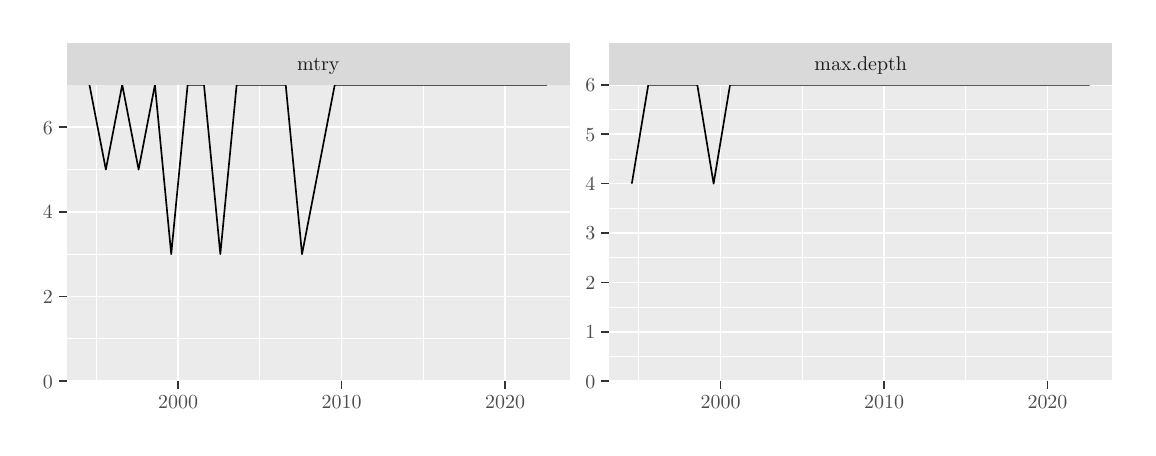
\begin{tikzpicture}[x=1pt,y=1pt]
\definecolor{fillColor}{RGB}{255,255,255}
\path[use as bounding box,fill=fillColor,fill opacity=0.00] (0,0) rectangle (397.48,144.54);
\begin{scope}
\path[clip] (  0.00,  0.00) rectangle (397.48,144.54);
\definecolor{drawColor}{RGB}{255,255,255}
\definecolor{fillColor}{RGB}{255,255,255}

\path[draw=drawColor,line width= 0.6pt,line join=round,line cap=round,fill=fillColor] (  0.00,  0.00) rectangle (397.48,144.54);
\end{scope}
\begin{scope}
\path[clip] ( 14.05, 16.81) rectangle (195.99,123.88);
\definecolor{fillColor}{gray}{0.92}

\path[fill=fillColor] ( 14.05, 16.81) rectangle (195.99,123.88);
\definecolor{drawColor}{RGB}{255,255,255}

\path[draw=drawColor,line width= 0.3pt,line join=round] ( 14.05, 32.10) --
	(195.99, 32.10);

\path[draw=drawColor,line width= 0.3pt,line join=round] ( 14.05, 62.70) --
	(195.99, 62.70);

\path[draw=drawColor,line width= 0.3pt,line join=round] ( 14.05, 93.29) --
	(195.99, 93.29);

\path[draw=drawColor,line width= 0.3pt,line join=round] ( 14.05,123.88) --
	(195.99,123.88);

\path[draw=drawColor,line width= 0.3pt,line join=round] ( 24.83, 16.81) --
	( 24.83,123.88);

\path[draw=drawColor,line width= 0.3pt,line join=round] ( 83.91, 16.81) --
	( 83.91,123.88);

\path[draw=drawColor,line width= 0.3pt,line join=round] (142.99, 16.81) --
	(142.99,123.88);

\path[draw=drawColor,line width= 0.6pt,line join=round] ( 14.05, 16.81) --
	(195.99, 16.81);

\path[draw=drawColor,line width= 0.6pt,line join=round] ( 14.05, 47.40) --
	(195.99, 47.40);

\path[draw=drawColor,line width= 0.6pt,line join=round] ( 14.05, 77.99) --
	(195.99, 77.99);

\path[draw=drawColor,line width= 0.6pt,line join=round] ( 14.05,108.59) --
	(195.99,108.59);

\path[draw=drawColor,line width= 0.6pt,line join=round] ( 54.37, 16.81) --
	( 54.37,123.88);

\path[draw=drawColor,line width= 0.6pt,line join=round] (113.46, 16.81) --
	(113.46,123.88);

\path[draw=drawColor,line width= 0.6pt,line join=round] (172.52, 16.81) --
	(172.52,123.88);
\definecolor{drawColor}{RGB}{0,0,0}

\path[draw=drawColor,line width= 0.6pt,line join=round] ( 22.32,123.88) --
	( 28.25, 93.29) --
	( 34.17,123.88) --
	( 40.08, 93.29) --
	( 45.98,123.88) --
	( 51.87, 62.70) --
	( 57.80,123.88) --
	( 63.71,123.88) --
	( 69.61, 62.70) --
	( 75.51,123.88) --
	( 81.42,123.88) --
	( 87.30,123.88) --
	( 93.24,123.88) --
	( 99.14, 62.70) --
	(105.06, 93.29) --
	(110.96,123.88) --
	(116.85,123.88) --
	(122.74,123.88) --
	(128.69,123.88) --
	(134.59,123.88) --
	(140.50,123.88) --
	(146.40,123.88) --
	(152.29,123.88) --
	(158.22,123.88) --
	(164.13,123.88) --
	(170.03,123.88) --
	(175.95,123.88) --
	(181.84,123.88) --
	(187.72,123.88);
\end{scope}
\begin{scope}
\path[clip] (210.04, 16.81) rectangle (391.98,123.88);
\definecolor{fillColor}{gray}{0.92}

\path[fill=fillColor] (210.04, 16.81) rectangle (391.98,123.88);
\definecolor{drawColor}{RGB}{255,255,255}

\path[draw=drawColor,line width= 0.3pt,line join=round] (210.04, 25.73) --
	(391.98, 25.73);

\path[draw=drawColor,line width= 0.3pt,line join=round] (210.04, 43.58) --
	(391.98, 43.58);

\path[draw=drawColor,line width= 0.3pt,line join=round] (210.04, 61.42) --
	(391.98, 61.42);

\path[draw=drawColor,line width= 0.3pt,line join=round] (210.04, 79.27) --
	(391.98, 79.27);

\path[draw=drawColor,line width= 0.3pt,line join=round] (210.04, 97.11) --
	(391.98, 97.11);

\path[draw=drawColor,line width= 0.3pt,line join=round] (210.04,114.96) --
	(391.98,114.96);

\path[draw=drawColor,line width= 0.3pt,line join=round] (220.83, 16.81) --
	(220.83,123.88);

\path[draw=drawColor,line width= 0.3pt,line join=round] (279.91, 16.81) --
	(279.91,123.88);

\path[draw=drawColor,line width= 0.3pt,line join=round] (338.98, 16.81) --
	(338.98,123.88);

\path[draw=drawColor,line width= 0.6pt,line join=round] (210.04, 16.81) --
	(391.98, 16.81);

\path[draw=drawColor,line width= 0.6pt,line join=round] (210.04, 34.65) --
	(391.98, 34.65);

\path[draw=drawColor,line width= 0.6pt,line join=round] (210.04, 52.50) --
	(391.98, 52.50);

\path[draw=drawColor,line width= 0.6pt,line join=round] (210.04, 70.34) --
	(391.98, 70.34);

\path[draw=drawColor,line width= 0.6pt,line join=round] (210.04, 88.19) --
	(391.98, 88.19);

\path[draw=drawColor,line width= 0.6pt,line join=round] (210.04,106.04) --
	(391.98,106.04);

\path[draw=drawColor,line width= 0.6pt,line join=round] (210.04,123.88) --
	(391.98,123.88);

\path[draw=drawColor,line width= 0.6pt,line join=round] (250.37, 16.81) --
	(250.37,123.88);

\path[draw=drawColor,line width= 0.6pt,line join=round] (309.45, 16.81) --
	(309.45,123.88);

\path[draw=drawColor,line width= 0.6pt,line join=round] (368.51, 16.81) --
	(368.51,123.88);
\definecolor{drawColor}{RGB}{0,0,0}

\path[draw=drawColor,line width= 0.6pt,line join=round] (218.31, 88.19) --
	(224.25,123.88) --
	(230.17,123.88) --
	(236.07,123.88) --
	(241.97,123.88) --
	(247.86, 88.19) --
	(253.80,123.88) --
	(259.70,123.88) --
	(265.60,123.88) --
	(271.51,123.88) --
	(277.41,123.88) --
	(283.30,123.88) --
	(289.23,123.88) --
	(295.13,123.88) --
	(301.05,123.88) --
	(306.96,123.88) --
	(312.84,123.88) --
	(318.73,123.88) --
	(324.68,123.88) --
	(330.59,123.88) --
	(336.49,123.88) --
	(342.39,123.88) --
	(348.28,123.88) --
	(354.21,123.88) --
	(360.12,123.88) --
	(366.02,123.88) --
	(371.94,123.88) --
	(377.83,123.88) --
	(383.71,123.88);
\end{scope}
\begin{scope}
\path[clip] ( 14.05,123.88) rectangle (195.99,139.04);
\definecolor{fillColor}{gray}{0.85}

\path[fill=fillColor] ( 14.05,123.88) rectangle (195.99,139.04);
\definecolor{drawColor}{gray}{0.10}

\node[text=drawColor,anchor=base,inner sep=0pt, outer sep=0pt, scale=  0.72] at (105.02,128.98) {mtry};
\end{scope}
\begin{scope}
\path[clip] (210.04,123.88) rectangle (391.98,139.04);
\definecolor{fillColor}{gray}{0.85}

\path[fill=fillColor] (210.04,123.88) rectangle (391.98,139.04);
\definecolor{drawColor}{gray}{0.10}

\node[text=drawColor,anchor=base,inner sep=0pt, outer sep=0pt, scale=  0.72] at (301.01,128.98) {max.depth};
\end{scope}
\begin{scope}
\path[clip] (  0.00,  0.00) rectangle (397.48,144.54);
\definecolor{drawColor}{gray}{0.20}

\path[draw=drawColor,line width= 0.6pt,line join=round] ( 54.37, 14.06) --
	( 54.37, 16.81);

\path[draw=drawColor,line width= 0.6pt,line join=round] (113.46, 14.06) --
	(113.46, 16.81);

\path[draw=drawColor,line width= 0.6pt,line join=round] (172.52, 14.06) --
	(172.52, 16.81);
\end{scope}
\begin{scope}
\path[clip] (  0.00,  0.00) rectangle (397.48,144.54);
\definecolor{drawColor}{gray}{0.30}

\node[text=drawColor,anchor=base,inner sep=0pt, outer sep=0pt, scale=  0.72] at ( 54.37,  6.90) {2000};

\node[text=drawColor,anchor=base,inner sep=0pt, outer sep=0pt, scale=  0.72] at (113.46,  6.90) {2010};

\node[text=drawColor,anchor=base,inner sep=0pt, outer sep=0pt, scale=  0.72] at (172.52,  6.90) {2020};
\end{scope}
\begin{scope}
\path[clip] (  0.00,  0.00) rectangle (397.48,144.54);
\definecolor{drawColor}{gray}{0.20}

\path[draw=drawColor,line width= 0.6pt,line join=round] (250.37, 14.06) --
	(250.37, 16.81);

\path[draw=drawColor,line width= 0.6pt,line join=round] (309.45, 14.06) --
	(309.45, 16.81);

\path[draw=drawColor,line width= 0.6pt,line join=round] (368.51, 14.06) --
	(368.51, 16.81);
\end{scope}
\begin{scope}
\path[clip] (  0.00,  0.00) rectangle (397.48,144.54);
\definecolor{drawColor}{gray}{0.30}

\node[text=drawColor,anchor=base,inner sep=0pt, outer sep=0pt, scale=  0.72] at (250.37,  6.90) {2000};

\node[text=drawColor,anchor=base,inner sep=0pt, outer sep=0pt, scale=  0.72] at (309.45,  6.90) {2010};

\node[text=drawColor,anchor=base,inner sep=0pt, outer sep=0pt, scale=  0.72] at (368.51,  6.90) {2020};
\end{scope}
\begin{scope}
\path[clip] (  0.00,  0.00) rectangle (397.48,144.54);
\definecolor{drawColor}{gray}{0.30}

\node[text=drawColor,anchor=base east,inner sep=0pt, outer sep=0pt, scale=  0.72] at (205.09, 14.33) {0};

\node[text=drawColor,anchor=base east,inner sep=0pt, outer sep=0pt, scale=  0.72] at (205.09, 32.17) {1};

\node[text=drawColor,anchor=base east,inner sep=0pt, outer sep=0pt, scale=  0.72] at (205.09, 50.02) {2};

\node[text=drawColor,anchor=base east,inner sep=0pt, outer sep=0pt, scale=  0.72] at (205.09, 67.87) {3};

\node[text=drawColor,anchor=base east,inner sep=0pt, outer sep=0pt, scale=  0.72] at (205.09, 85.71) {4};

\node[text=drawColor,anchor=base east,inner sep=0pt, outer sep=0pt, scale=  0.72] at (205.09,103.56) {5};

\node[text=drawColor,anchor=base east,inner sep=0pt, outer sep=0pt, scale=  0.72] at (205.09,121.40) {6};
\end{scope}
\begin{scope}
\path[clip] (  0.00,  0.00) rectangle (397.48,144.54);
\definecolor{drawColor}{gray}{0.20}

\path[draw=drawColor,line width= 0.6pt,line join=round] (207.29, 16.81) --
	(210.04, 16.81);

\path[draw=drawColor,line width= 0.6pt,line join=round] (207.29, 34.65) --
	(210.04, 34.65);

\path[draw=drawColor,line width= 0.6pt,line join=round] (207.29, 52.50) --
	(210.04, 52.50);

\path[draw=drawColor,line width= 0.6pt,line join=round] (207.29, 70.34) --
	(210.04, 70.34);

\path[draw=drawColor,line width= 0.6pt,line join=round] (207.29, 88.19) --
	(210.04, 88.19);

\path[draw=drawColor,line width= 0.6pt,line join=round] (207.29,106.04) --
	(210.04,106.04);

\path[draw=drawColor,line width= 0.6pt,line join=round] (207.29,123.88) --
	(210.04,123.88);
\end{scope}
\begin{scope}
\path[clip] (  0.00,  0.00) rectangle (397.48,144.54);
\definecolor{drawColor}{gray}{0.30}

\node[text=drawColor,anchor=base east,inner sep=0pt, outer sep=0pt, scale=  0.72] at (  9.10, 14.33) {0};

\node[text=drawColor,anchor=base east,inner sep=0pt, outer sep=0pt, scale=  0.72] at (  9.10, 44.92) {2};

\node[text=drawColor,anchor=base east,inner sep=0pt, outer sep=0pt, scale=  0.72] at (  9.10, 75.51) {4};

\node[text=drawColor,anchor=base east,inner sep=0pt, outer sep=0pt, scale=  0.72] at (  9.10,106.11) {6};
\end{scope}
\begin{scope}
\path[clip] (  0.00,  0.00) rectangle (397.48,144.54);
\definecolor{drawColor}{gray}{0.20}

\path[draw=drawColor,line width= 0.6pt,line join=round] ( 11.30, 16.81) --
	( 14.05, 16.81);

\path[draw=drawColor,line width= 0.6pt,line join=round] ( 11.30, 47.40) --
	( 14.05, 47.40);

\path[draw=drawColor,line width= 0.6pt,line join=round] ( 11.30, 77.99) --
	( 14.05, 77.99);

\path[draw=drawColor,line width= 0.6pt,line join=round] ( 11.30,108.59) --
	( 14.05,108.59);
\end{scope}
\end{tikzpicture}

\label{plot:RFHyperParams}
\end{figure}

\begin{figure}[h]
\centering
\caption[Turnover of highest epected return portfolios]{\textbf{Turnover of highest epected return portfolios}\\ .}
% Created by tikzDevice version 0.12.6 on 2024-03-11 18:45:03
% !TEX encoding = UTF-8 Unicode
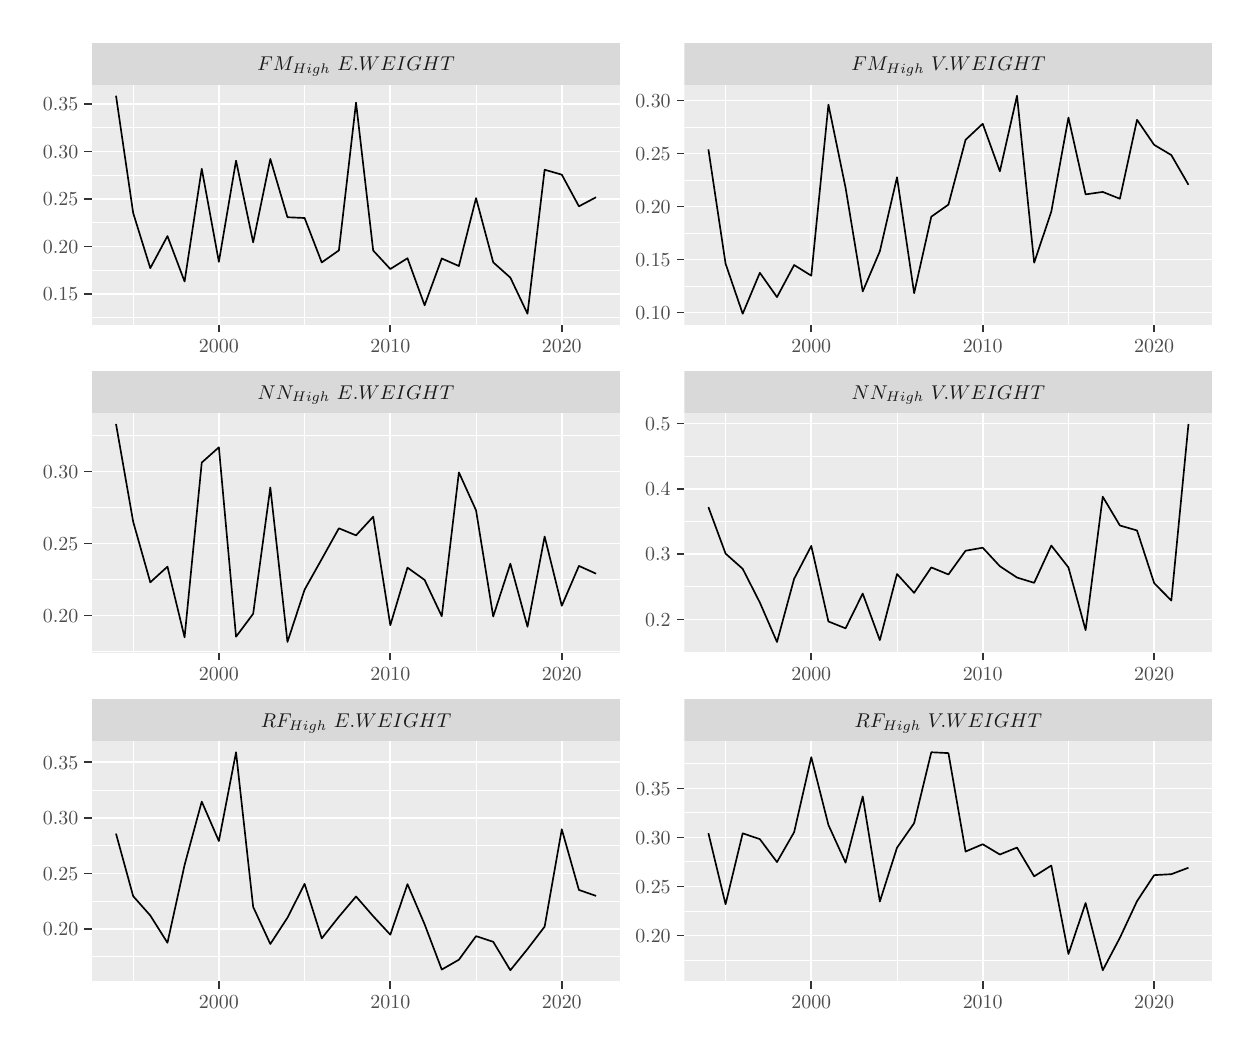
\begin{tikzpicture}[x=1pt,y=1pt]
\definecolor{fillColor}{RGB}{255,255,255}
\path[use as bounding box,fill=fillColor,fill opacity=0.00] (0,0) rectangle (433.62,361.35);
\begin{scope}
\path[clip] (  0.00,  0.00) rectangle (433.62,361.35);
\definecolor{drawColor}{RGB}{255,255,255}
\definecolor{fillColor}{RGB}{255,255,255}

\path[draw=drawColor,line width= 0.6pt,line join=round,line cap=round,fill=fillColor] (  0.00,  0.00) rectangle (433.62,361.35);
\end{scope}
\begin{scope}
\path[clip] ( 23.25,254.04) rectangle (214.06,340.69);
\definecolor{fillColor}{gray}{0.92}

\path[fill=fillColor] ( 23.25,254.04) rectangle (214.06,340.69);
\definecolor{drawColor}{RGB}{255,255,255}

\path[draw=drawColor,line width= 0.3pt,line join=round] ( 23.25,256.50) --
	(214.06,256.50);

\path[draw=drawColor,line width= 0.3pt,line join=round] ( 23.25,273.67) --
	(214.06,273.67);

\path[draw=drawColor,line width= 0.3pt,line join=round] ( 23.25,290.84) --
	(214.06,290.84);

\path[draw=drawColor,line width= 0.3pt,line join=round] ( 23.25,308.01) --
	(214.06,308.01);

\path[draw=drawColor,line width= 0.3pt,line join=round] ( 23.25,325.18) --
	(214.06,325.18);

\path[draw=drawColor,line width= 0.3pt,line join=round] ( 38.12,254.04) --
	( 38.12,340.69);

\path[draw=drawColor,line width= 0.3pt,line join=round] (100.07,254.04) --
	(100.07,340.69);

\path[draw=drawColor,line width= 0.3pt,line join=round] (162.02,254.04) --
	(162.02,340.69);

\path[draw=drawColor,line width= 0.6pt,line join=round] ( 23.25,265.09) --
	(214.06,265.09);

\path[draw=drawColor,line width= 0.6pt,line join=round] ( 23.25,282.26) --
	(214.06,282.26);

\path[draw=drawColor,line width= 0.6pt,line join=round] ( 23.25,299.43) --
	(214.06,299.43);

\path[draw=drawColor,line width= 0.6pt,line join=round] ( 23.25,316.60) --
	(214.06,316.60);

\path[draw=drawColor,line width= 0.6pt,line join=round] ( 23.25,333.77) --
	(214.06,333.77);

\path[draw=drawColor,line width= 0.6pt,line join=round] ( 69.09,254.04) --
	( 69.09,340.69);

\path[draw=drawColor,line width= 0.6pt,line join=round] (131.04,254.04) --
	(131.04,340.69);

\path[draw=drawColor,line width= 0.6pt,line join=round] (193.00,254.04) --
	(193.00,340.69);
\definecolor{drawColor}{RGB}{0,0,0}

\path[draw=drawColor,line width= 0.6pt,line join=round] ( 31.92,336.75) --
	( 38.12,294.39) --
	( 44.31,274.45) --
	( 50.51,286.04) --
	( 56.70,269.63) --
	( 62.90,310.37) --
	( 69.09,276.73) --
	( 75.29,313.29) --
	( 81.48,283.78) --
	( 87.68,313.91) --
	( 93.87,292.85) --
	(100.07,292.57) --
	(106.26,276.51) --
	(112.46,280.87) --
	(118.65,334.26) --
	(124.85,280.82) --
	(131.04,274.13) --
	(137.24,278.03) --
	(143.43,261.03) --
	(149.63,277.94) --
	(155.82,275.22) --
	(162.02,299.75) --
	(168.22,276.55) --
	(174.41,271.03) --
	(180.61,257.98) --
	(186.80,310.01) --
	(193.00,308.24) --
	(199.19,296.79) --
	(205.39,300.07);
\end{scope}
\begin{scope}
\path[clip] ( 23.25,135.43) rectangle (214.06,222.07);
\definecolor{fillColor}{gray}{0.92}

\path[fill=fillColor] ( 23.25,135.43) rectangle (214.06,222.07);
\definecolor{drawColor}{RGB}{255,255,255}

\path[draw=drawColor,line width= 0.3pt,line join=round] ( 23.25,135.94) --
	(214.06,135.94);

\path[draw=drawColor,line width= 0.3pt,line join=round] ( 23.25,161.96) --
	(214.06,161.96);

\path[draw=drawColor,line width= 0.3pt,line join=round] ( 23.25,187.98) --
	(214.06,187.98);

\path[draw=drawColor,line width= 0.3pt,line join=round] ( 23.25,214.00) --
	(214.06,214.00);

\path[draw=drawColor,line width= 0.3pt,line join=round] ( 38.12,135.43) --
	( 38.12,222.07);

\path[draw=drawColor,line width= 0.3pt,line join=round] (100.07,135.43) --
	(100.07,222.07);

\path[draw=drawColor,line width= 0.3pt,line join=round] (162.02,135.43) --
	(162.02,222.07);

\path[draw=drawColor,line width= 0.6pt,line join=round] ( 23.25,148.95) --
	(214.06,148.95);

\path[draw=drawColor,line width= 0.6pt,line join=round] ( 23.25,174.97) --
	(214.06,174.97);

\path[draw=drawColor,line width= 0.6pt,line join=round] ( 23.25,200.99) --
	(214.06,200.99);

\path[draw=drawColor,line width= 0.6pt,line join=round] ( 69.09,135.43) --
	( 69.09,222.07);

\path[draw=drawColor,line width= 0.6pt,line join=round] (131.04,135.43) --
	(131.04,222.07);

\path[draw=drawColor,line width= 0.6pt,line join=round] (193.00,135.43) --
	(193.00,222.07);
\definecolor{drawColor}{RGB}{0,0,0}

\path[draw=drawColor,line width= 0.6pt,line join=round] ( 31.92,218.14) --
	( 38.12,182.84) --
	( 44.31,160.94) --
	( 50.51,166.59) --
	( 56.70,141.06) --
	( 62.90,204.19) --
	( 69.09,209.72) --
	( 75.29,141.28) --
	( 81.48,149.55) --
	( 87.68,195.19) --
	( 93.87,139.36) --
	(100.07,158.28) --
	(106.26,169.32) --
	(112.46,180.45) --
	(118.65,177.89) --
	(124.85,184.63) --
	(131.04,145.43) --
	(137.24,166.23) --
	(143.43,161.79) --
	(149.63,148.67) --
	(155.82,200.65) --
	(162.02,186.92) --
	(168.22,148.57) --
	(174.41,167.65) --
	(180.61,144.88) --
	(186.80,177.47) --
	(193.00,152.44) --
	(199.19,166.85) --
	(205.39,164.05);
\end{scope}
\begin{scope}
\path[clip] ( 23.25, 16.81) rectangle (214.06,103.46);
\definecolor{fillColor}{gray}{0.92}

\path[fill=fillColor] ( 23.25, 16.81) rectangle (214.06,103.46);
\definecolor{drawColor}{RGB}{255,255,255}

\path[draw=drawColor,line width= 0.3pt,line join=round] ( 23.25, 25.58) --
	(214.06, 25.58);

\path[draw=drawColor,line width= 0.3pt,line join=round] ( 23.25, 45.68) --
	(214.06, 45.68);

\path[draw=drawColor,line width= 0.3pt,line join=round] ( 23.25, 65.79) --
	(214.06, 65.79);

\path[draw=drawColor,line width= 0.3pt,line join=round] ( 23.25, 85.89) --
	(214.06, 85.89);

\path[draw=drawColor,line width= 0.3pt,line join=round] ( 38.12, 16.81) --
	( 38.12,103.46);

\path[draw=drawColor,line width= 0.3pt,line join=round] (100.07, 16.81) --
	(100.07,103.46);

\path[draw=drawColor,line width= 0.3pt,line join=round] (162.02, 16.81) --
	(162.02,103.46);

\path[draw=drawColor,line width= 0.6pt,line join=round] ( 23.25, 35.63) --
	(214.06, 35.63);

\path[draw=drawColor,line width= 0.6pt,line join=round] ( 23.25, 55.74) --
	(214.06, 55.74);

\path[draw=drawColor,line width= 0.6pt,line join=round] ( 23.25, 75.84) --
	(214.06, 75.84);

\path[draw=drawColor,line width= 0.6pt,line join=round] ( 23.25, 95.95) --
	(214.06, 95.95);

\path[draw=drawColor,line width= 0.6pt,line join=round] ( 69.09, 16.81) --
	( 69.09,103.46);

\path[draw=drawColor,line width= 0.6pt,line join=round] (131.04, 16.81) --
	(131.04,103.46);

\path[draw=drawColor,line width= 0.6pt,line join=round] (193.00, 16.81) --
	(193.00,103.46);
\definecolor{drawColor}{RGB}{0,0,0}

\path[draw=drawColor,line width= 0.6pt,line join=round] ( 31.92, 70.11) --
	( 38.12, 47.52) --
	( 44.31, 40.53) --
	( 50.51, 30.68) --
	( 56.70, 58.79) --
	( 62.90, 81.69) --
	( 69.09, 67.43) --
	( 75.29, 99.52) --
	( 81.48, 43.63) --
	( 87.68, 30.23) --
	( 93.87, 39.73) --
	(100.07, 51.96) --
	(106.26, 32.26) --
	(112.46, 40.08) --
	(118.65, 47.41) --
	(124.85, 40.28) --
	(131.04, 33.60) --
	(137.24, 51.86) --
	(143.43, 37.36) --
	(149.63, 21.00) --
	(155.82, 24.55) --
	(162.02, 33.07) --
	(168.22, 31.04) --
	(174.41, 20.75) --
	(180.61, 28.41) --
	(186.80, 36.51) --
	(193.00, 71.68) --
	(199.19, 49.78) --
	(205.39, 47.61);
\end{scope}
\begin{scope}
\path[clip] (237.31,254.04) rectangle (428.12,340.69);
\definecolor{fillColor}{gray}{0.92}

\path[fill=fillColor] (237.31,254.04) rectangle (428.12,340.69);
\definecolor{drawColor}{RGB}{255,255,255}

\path[draw=drawColor,line width= 0.3pt,line join=round] (237.31,267.96) --
	(428.12,267.96);

\path[draw=drawColor,line width= 0.3pt,line join=round] (237.31,287.11) --
	(428.12,287.11);

\path[draw=drawColor,line width= 0.3pt,line join=round] (237.31,306.27) --
	(428.12,306.27);

\path[draw=drawColor,line width= 0.3pt,line join=round] (237.31,325.43) --
	(428.12,325.43);

\path[draw=drawColor,line width= 0.3pt,line join=round] (252.18,254.04) --
	(252.18,340.69);

\path[draw=drawColor,line width= 0.3pt,line join=round] (314.13,254.04) --
	(314.13,340.69);

\path[draw=drawColor,line width= 0.3pt,line join=round] (376.08,254.04) --
	(376.08,340.69);

\path[draw=drawColor,line width= 0.6pt,line join=round] (237.31,258.38) --
	(428.12,258.38);

\path[draw=drawColor,line width= 0.6pt,line join=round] (237.31,277.53) --
	(428.12,277.53);

\path[draw=drawColor,line width= 0.6pt,line join=round] (237.31,296.69) --
	(428.12,296.69);

\path[draw=drawColor,line width= 0.6pt,line join=round] (237.31,315.85) --
	(428.12,315.85);

\path[draw=drawColor,line width= 0.6pt,line join=round] (237.31,335.01) --
	(428.12,335.01);

\path[draw=drawColor,line width= 0.6pt,line join=round] (283.15,254.04) --
	(283.15,340.69);

\path[draw=drawColor,line width= 0.6pt,line join=round] (345.10,254.04) --
	(345.10,340.69);

\path[draw=drawColor,line width= 0.6pt,line join=round] (407.06,254.04) --
	(407.06,340.69);
\definecolor{drawColor}{RGB}{0,0,0}

\path[draw=drawColor,line width= 0.6pt,line join=round] (245.98,317.36) --
	(252.18,276.08) --
	(258.37,257.98) --
	(264.57,272.78) --
	(270.76,263.99) --
	(276.96,275.58) --
	(283.15,271.73) --
	(289.35,333.54) --
	(295.54,303.51) --
	(301.74,266.03) --
	(307.93,280.56) --
	(314.13,307.29) --
	(320.32,265.40) --
	(326.52,293.04) --
	(332.71,297.41) --
	(338.91,320.83) --
	(345.10,326.62) --
	(351.30,309.44) --
	(357.49,336.75) --
	(363.69,276.42) --
	(369.88,294.86) --
	(376.08,328.86) --
	(382.28,301.11) --
	(388.47,301.99) --
	(394.67,299.53) --
	(400.86,328.05) --
	(407.06,318.99) --
	(413.25,315.31) --
	(419.45,304.57);
\end{scope}
\begin{scope}
\path[clip] (237.31,135.43) rectangle (428.12,222.07);
\definecolor{fillColor}{gray}{0.92}

\path[fill=fillColor] (237.31,135.43) rectangle (428.12,222.07);
\definecolor{drawColor}{RGB}{255,255,255}

\path[draw=drawColor,line width= 0.3pt,line join=round] (237.31,135.76) --
	(428.12,135.76);

\path[draw=drawColor,line width= 0.3pt,line join=round] (237.31,159.34) --
	(428.12,159.34);

\path[draw=drawColor,line width= 0.3pt,line join=round] (237.31,182.91) --
	(428.12,182.91);

\path[draw=drawColor,line width= 0.3pt,line join=round] (237.31,206.49) --
	(428.12,206.49);

\path[draw=drawColor,line width= 0.3pt,line join=round] (252.18,135.43) --
	(252.18,222.07);

\path[draw=drawColor,line width= 0.3pt,line join=round] (314.13,135.43) --
	(314.13,222.07);

\path[draw=drawColor,line width= 0.3pt,line join=round] (376.08,135.43) --
	(376.08,222.07);

\path[draw=drawColor,line width= 0.6pt,line join=round] (237.31,147.55) --
	(428.12,147.55);

\path[draw=drawColor,line width= 0.6pt,line join=round] (237.31,171.12) --
	(428.12,171.12);

\path[draw=drawColor,line width= 0.6pt,line join=round] (237.31,194.70) --
	(428.12,194.70);

\path[draw=drawColor,line width= 0.6pt,line join=round] (237.31,218.28) --
	(428.12,218.28);

\path[draw=drawColor,line width= 0.6pt,line join=round] (283.15,135.43) --
	(283.15,222.07);

\path[draw=drawColor,line width= 0.6pt,line join=round] (345.10,135.43) --
	(345.10,222.07);

\path[draw=drawColor,line width= 0.6pt,line join=round] (407.06,135.43) --
	(407.06,222.07);
\definecolor{drawColor}{RGB}{0,0,0}

\path[draw=drawColor,line width= 0.6pt,line join=round] (245.98,188.10) --
	(252.18,171.31) --
	(258.37,165.80) --
	(264.57,153.62) --
	(270.76,139.36) --
	(276.96,162.21) --
	(283.15,174.08) --
	(289.35,146.78) --
	(295.54,144.30) --
	(301.74,156.87) --
	(307.93,140.03) --
	(314.13,163.93) --
	(320.32,157.12) --
	(326.52,166.31) --
	(332.71,163.76) --
	(338.91,172.34) --
	(345.10,173.43) --
	(351.30,166.74) --
	(357.49,162.65) --
	(363.69,160.74) --
	(369.88,174.21) --
	(376.08,166.30) --
	(382.28,143.64) --
	(388.47,191.87) --
	(394.67,181.46) --
	(400.86,179.66) --
	(407.06,160.62) --
	(413.25,154.33) --
	(419.45,218.14);
\end{scope}
\begin{scope}
\path[clip] (237.31, 16.81) rectangle (428.12,103.46);
\definecolor{fillColor}{gray}{0.92}

\path[fill=fillColor] (237.31, 16.81) rectangle (428.12,103.46);
\definecolor{drawColor}{RGB}{255,255,255}

\path[draw=drawColor,line width= 0.3pt,line join=round] (237.31, 24.46) --
	(428.12, 24.46);

\path[draw=drawColor,line width= 0.3pt,line join=round] (237.31, 42.18) --
	(428.12, 42.18);

\path[draw=drawColor,line width= 0.3pt,line join=round] (237.31, 59.90) --
	(428.12, 59.90);

\path[draw=drawColor,line width= 0.3pt,line join=round] (237.31, 77.62) --
	(428.12, 77.62);

\path[draw=drawColor,line width= 0.3pt,line join=round] (237.31, 95.34) --
	(428.12, 95.34);

\path[draw=drawColor,line width= 0.3pt,line join=round] (252.18, 16.81) --
	(252.18,103.46);

\path[draw=drawColor,line width= 0.3pt,line join=round] (314.13, 16.81) --
	(314.13,103.46);

\path[draw=drawColor,line width= 0.3pt,line join=round] (376.08, 16.81) --
	(376.08,103.46);

\path[draw=drawColor,line width= 0.6pt,line join=round] (237.31, 33.32) --
	(428.12, 33.32);

\path[draw=drawColor,line width= 0.6pt,line join=round] (237.31, 51.04) --
	(428.12, 51.04);

\path[draw=drawColor,line width= 0.6pt,line join=round] (237.31, 68.76) --
	(428.12, 68.76);

\path[draw=drawColor,line width= 0.6pt,line join=round] (237.31, 86.48) --
	(428.12, 86.48);

\path[draw=drawColor,line width= 0.6pt,line join=round] (283.15, 16.81) --
	(283.15,103.46);

\path[draw=drawColor,line width= 0.6pt,line join=round] (345.10, 16.81) --
	(345.10,103.46);

\path[draw=drawColor,line width= 0.6pt,line join=round] (407.06, 16.81) --
	(407.06,103.46);
\definecolor{drawColor}{RGB}{0,0,0}

\path[draw=drawColor,line width= 0.6pt,line join=round] (245.98, 70.27) --
	(252.18, 44.61) --
	(258.37, 70.23) --
	(264.57, 68.12) --
	(270.76, 59.84) --
	(276.96, 70.65) --
	(283.15, 97.74) --
	(289.35, 73.24) --
	(295.54, 59.62) --
	(301.74, 83.56) --
	(307.93, 45.60) --
	(314.13, 65.03) --
	(320.32, 73.91) --
	(326.52, 99.52) --
	(332.71, 99.21) --
	(338.91, 63.65) --
	(345.10, 66.28) --
	(351.30, 62.57) --
	(357.49, 65.08) --
	(363.69, 54.68) --
	(369.88, 58.59) --
	(376.08, 26.62) --
	(382.28, 45.05) --
	(388.47, 20.75) --
	(394.67, 32.48) --
	(400.86, 45.72) --
	(407.06, 55.12) --
	(413.25, 55.46) --
	(419.45, 57.80);
\end{scope}
\begin{scope}
\path[clip] ( 23.25,103.46) rectangle (214.06,118.62);
\definecolor{fillColor}{gray}{0.85}

\path[fill=fillColor] ( 23.25,103.46) rectangle (214.06,118.62);
\definecolor{drawColor}{gray}{0.10}

\node[text=drawColor,anchor=base,inner sep=0pt, outer sep=0pt, scale=  0.72] at (118.65,108.56) {$ RF _{ High } \ E.WEIGHT $};
\end{scope}
\begin{scope}
\path[clip] (237.31,103.46) rectangle (428.12,118.62);
\definecolor{fillColor}{gray}{0.85}

\path[fill=fillColor] (237.31,103.46) rectangle (428.12,118.62);
\definecolor{drawColor}{gray}{0.10}

\node[text=drawColor,anchor=base,inner sep=0pt, outer sep=0pt, scale=  0.72] at (332.71,108.56) {$ RF _{ High } \ V.WEIGHT $};
\end{scope}
\begin{scope}
\path[clip] ( 23.25,222.07) rectangle (214.06,237.23);
\definecolor{fillColor}{gray}{0.85}

\path[fill=fillColor] ( 23.25,222.07) rectangle (214.06,237.23);
\definecolor{drawColor}{gray}{0.10}

\node[text=drawColor,anchor=base,inner sep=0pt, outer sep=0pt, scale=  0.72] at (118.65,227.17) {$ NN _{ High } \ E.WEIGHT $};
\end{scope}
\begin{scope}
\path[clip] (237.31,222.07) rectangle (428.12,237.23);
\definecolor{fillColor}{gray}{0.85}

\path[fill=fillColor] (237.31,222.07) rectangle (428.12,237.23);
\definecolor{drawColor}{gray}{0.10}

\node[text=drawColor,anchor=base,inner sep=0pt, outer sep=0pt, scale=  0.72] at (332.71,227.17) {$ NN _{ High } \ V.WEIGHT $};
\end{scope}
\begin{scope}
\path[clip] ( 23.25,340.69) rectangle (214.06,355.85);
\definecolor{fillColor}{gray}{0.85}

\path[fill=fillColor] ( 23.25,340.69) rectangle (214.06,355.85);
\definecolor{drawColor}{gray}{0.10}

\node[text=drawColor,anchor=base,inner sep=0pt, outer sep=0pt, scale=  0.72] at (118.65,345.79) {$ FM _{ High } \ E.WEIGHT $};
\end{scope}
\begin{scope}
\path[clip] (237.31,340.69) rectangle (428.12,355.85);
\definecolor{fillColor}{gray}{0.85}

\path[fill=fillColor] (237.31,340.69) rectangle (428.12,355.85);
\definecolor{drawColor}{gray}{0.10}

\node[text=drawColor,anchor=base,inner sep=0pt, outer sep=0pt, scale=  0.72] at (332.71,345.79) {$ FM _{ High } \ V.WEIGHT $};
\end{scope}
\begin{scope}
\path[clip] (  0.00,  0.00) rectangle (433.62,361.35);
\definecolor{drawColor}{gray}{0.20}

\path[draw=drawColor,line width= 0.6pt,line join=round] ( 69.09, 14.06) --
	( 69.09, 16.81);

\path[draw=drawColor,line width= 0.6pt,line join=round] (131.04, 14.06) --
	(131.04, 16.81);

\path[draw=drawColor,line width= 0.6pt,line join=round] (193.00, 14.06) --
	(193.00, 16.81);
\end{scope}
\begin{scope}
\path[clip] (  0.00,  0.00) rectangle (433.62,361.35);
\definecolor{drawColor}{gray}{0.30}

\node[text=drawColor,anchor=base,inner sep=0pt, outer sep=0pt, scale=  0.72] at ( 69.09,  6.90) {2000};

\node[text=drawColor,anchor=base,inner sep=0pt, outer sep=0pt, scale=  0.72] at (131.04,  6.90) {2010};

\node[text=drawColor,anchor=base,inner sep=0pt, outer sep=0pt, scale=  0.72] at (193.00,  6.90) {2020};
\end{scope}
\begin{scope}
\path[clip] (  0.00,  0.00) rectangle (433.62,361.35);
\definecolor{drawColor}{gray}{0.20}

\path[draw=drawColor,line width= 0.6pt,line join=round] (283.15, 14.06) --
	(283.15, 16.81);

\path[draw=drawColor,line width= 0.6pt,line join=round] (345.10, 14.06) --
	(345.10, 16.81);

\path[draw=drawColor,line width= 0.6pt,line join=round] (407.06, 14.06) --
	(407.06, 16.81);
\end{scope}
\begin{scope}
\path[clip] (  0.00,  0.00) rectangle (433.62,361.35);
\definecolor{drawColor}{gray}{0.30}

\node[text=drawColor,anchor=base,inner sep=0pt, outer sep=0pt, scale=  0.72] at (283.15,  6.90) {2000};

\node[text=drawColor,anchor=base,inner sep=0pt, outer sep=0pt, scale=  0.72] at (345.10,  6.90) {2010};

\node[text=drawColor,anchor=base,inner sep=0pt, outer sep=0pt, scale=  0.72] at (407.06,  6.90) {2020};
\end{scope}
\begin{scope}
\path[clip] (  0.00,  0.00) rectangle (433.62,361.35);
\definecolor{drawColor}{gray}{0.20}

\path[draw=drawColor,line width= 0.6pt,line join=round] ( 69.09,132.68) --
	( 69.09,135.43);

\path[draw=drawColor,line width= 0.6pt,line join=round] (131.04,132.68) --
	(131.04,135.43);

\path[draw=drawColor,line width= 0.6pt,line join=round] (193.00,132.68) --
	(193.00,135.43);
\end{scope}
\begin{scope}
\path[clip] (  0.00,  0.00) rectangle (433.62,361.35);
\definecolor{drawColor}{gray}{0.30}

\node[text=drawColor,anchor=base,inner sep=0pt, outer sep=0pt, scale=  0.72] at ( 69.09,125.52) {2000};

\node[text=drawColor,anchor=base,inner sep=0pt, outer sep=0pt, scale=  0.72] at (131.04,125.52) {2010};

\node[text=drawColor,anchor=base,inner sep=0pt, outer sep=0pt, scale=  0.72] at (193.00,125.52) {2020};
\end{scope}
\begin{scope}
\path[clip] (  0.00,  0.00) rectangle (433.62,361.35);
\definecolor{drawColor}{gray}{0.20}

\path[draw=drawColor,line width= 0.6pt,line join=round] (283.15,132.68) --
	(283.15,135.43);

\path[draw=drawColor,line width= 0.6pt,line join=round] (345.10,132.68) --
	(345.10,135.43);

\path[draw=drawColor,line width= 0.6pt,line join=round] (407.06,132.68) --
	(407.06,135.43);
\end{scope}
\begin{scope}
\path[clip] (  0.00,  0.00) rectangle (433.62,361.35);
\definecolor{drawColor}{gray}{0.30}

\node[text=drawColor,anchor=base,inner sep=0pt, outer sep=0pt, scale=  0.72] at (283.15,125.52) {2000};

\node[text=drawColor,anchor=base,inner sep=0pt, outer sep=0pt, scale=  0.72] at (345.10,125.52) {2010};

\node[text=drawColor,anchor=base,inner sep=0pt, outer sep=0pt, scale=  0.72] at (407.06,125.52) {2020};
\end{scope}
\begin{scope}
\path[clip] (  0.00,  0.00) rectangle (433.62,361.35);
\definecolor{drawColor}{gray}{0.20}

\path[draw=drawColor,line width= 0.6pt,line join=round] ( 69.09,251.29) --
	( 69.09,254.04);

\path[draw=drawColor,line width= 0.6pt,line join=round] (131.04,251.29) --
	(131.04,254.04);

\path[draw=drawColor,line width= 0.6pt,line join=round] (193.00,251.29) --
	(193.00,254.04);
\end{scope}
\begin{scope}
\path[clip] (  0.00,  0.00) rectangle (433.62,361.35);
\definecolor{drawColor}{gray}{0.30}

\node[text=drawColor,anchor=base,inner sep=0pt, outer sep=0pt, scale=  0.72] at ( 69.09,244.13) {2000};

\node[text=drawColor,anchor=base,inner sep=0pt, outer sep=0pt, scale=  0.72] at (131.04,244.13) {2010};

\node[text=drawColor,anchor=base,inner sep=0pt, outer sep=0pt, scale=  0.72] at (193.00,244.13) {2020};
\end{scope}
\begin{scope}
\path[clip] (  0.00,  0.00) rectangle (433.62,361.35);
\definecolor{drawColor}{gray}{0.20}

\path[draw=drawColor,line width= 0.6pt,line join=round] (283.15,251.29) --
	(283.15,254.04);

\path[draw=drawColor,line width= 0.6pt,line join=round] (345.10,251.29) --
	(345.10,254.04);

\path[draw=drawColor,line width= 0.6pt,line join=round] (407.06,251.29) --
	(407.06,254.04);
\end{scope}
\begin{scope}
\path[clip] (  0.00,  0.00) rectangle (433.62,361.35);
\definecolor{drawColor}{gray}{0.30}

\node[text=drawColor,anchor=base,inner sep=0pt, outer sep=0pt, scale=  0.72] at (283.15,244.13) {2000};

\node[text=drawColor,anchor=base,inner sep=0pt, outer sep=0pt, scale=  0.72] at (345.10,244.13) {2010};

\node[text=drawColor,anchor=base,inner sep=0pt, outer sep=0pt, scale=  0.72] at (407.06,244.13) {2020};
\end{scope}
\begin{scope}
\path[clip] (  0.00,  0.00) rectangle (433.62,361.35);
\definecolor{drawColor}{gray}{0.30}

\node[text=drawColor,anchor=base east,inner sep=0pt, outer sep=0pt, scale=  0.72] at (232.36,255.90) {0.10};

\node[text=drawColor,anchor=base east,inner sep=0pt, outer sep=0pt, scale=  0.72] at (232.36,275.05) {0.15};

\node[text=drawColor,anchor=base east,inner sep=0pt, outer sep=0pt, scale=  0.72] at (232.36,294.21) {0.20};

\node[text=drawColor,anchor=base east,inner sep=0pt, outer sep=0pt, scale=  0.72] at (232.36,313.37) {0.25};

\node[text=drawColor,anchor=base east,inner sep=0pt, outer sep=0pt, scale=  0.72] at (232.36,332.53) {0.30};
\end{scope}
\begin{scope}
\path[clip] (  0.00,  0.00) rectangle (433.62,361.35);
\definecolor{drawColor}{gray}{0.20}

\path[draw=drawColor,line width= 0.6pt,line join=round] (234.56,258.38) --
	(237.31,258.38);

\path[draw=drawColor,line width= 0.6pt,line join=round] (234.56,277.53) --
	(237.31,277.53);

\path[draw=drawColor,line width= 0.6pt,line join=round] (234.56,296.69) --
	(237.31,296.69);

\path[draw=drawColor,line width= 0.6pt,line join=round] (234.56,315.85) --
	(237.31,315.85);

\path[draw=drawColor,line width= 0.6pt,line join=round] (234.56,335.01) --
	(237.31,335.01);
\end{scope}
\begin{scope}
\path[clip] (  0.00,  0.00) rectangle (433.62,361.35);
\definecolor{drawColor}{gray}{0.30}

\node[text=drawColor,anchor=base east,inner sep=0pt, outer sep=0pt, scale=  0.72] at (232.36,145.07) {0.2};

\node[text=drawColor,anchor=base east,inner sep=0pt, outer sep=0pt, scale=  0.72] at (232.36,168.65) {0.3};

\node[text=drawColor,anchor=base east,inner sep=0pt, outer sep=0pt, scale=  0.72] at (232.36,192.22) {0.4};

\node[text=drawColor,anchor=base east,inner sep=0pt, outer sep=0pt, scale=  0.72] at (232.36,215.80) {0.5};
\end{scope}
\begin{scope}
\path[clip] (  0.00,  0.00) rectangle (433.62,361.35);
\definecolor{drawColor}{gray}{0.20}

\path[draw=drawColor,line width= 0.6pt,line join=round] (234.56,147.55) --
	(237.31,147.55);

\path[draw=drawColor,line width= 0.6pt,line join=round] (234.56,171.12) --
	(237.31,171.12);

\path[draw=drawColor,line width= 0.6pt,line join=round] (234.56,194.70) --
	(237.31,194.70);

\path[draw=drawColor,line width= 0.6pt,line join=round] (234.56,218.28) --
	(237.31,218.28);
\end{scope}
\begin{scope}
\path[clip] (  0.00,  0.00) rectangle (433.62,361.35);
\definecolor{drawColor}{gray}{0.30}

\node[text=drawColor,anchor=base east,inner sep=0pt, outer sep=0pt, scale=  0.72] at (232.36, 30.84) {0.20};

\node[text=drawColor,anchor=base east,inner sep=0pt, outer sep=0pt, scale=  0.72] at (232.36, 48.56) {0.25};

\node[text=drawColor,anchor=base east,inner sep=0pt, outer sep=0pt, scale=  0.72] at (232.36, 66.28) {0.30};

\node[text=drawColor,anchor=base east,inner sep=0pt, outer sep=0pt, scale=  0.72] at (232.36, 84.00) {0.35};
\end{scope}
\begin{scope}
\path[clip] (  0.00,  0.00) rectangle (433.62,361.35);
\definecolor{drawColor}{gray}{0.20}

\path[draw=drawColor,line width= 0.6pt,line join=round] (234.56, 33.32) --
	(237.31, 33.32);

\path[draw=drawColor,line width= 0.6pt,line join=round] (234.56, 51.04) --
	(237.31, 51.04);

\path[draw=drawColor,line width= 0.6pt,line join=round] (234.56, 68.76) --
	(237.31, 68.76);

\path[draw=drawColor,line width= 0.6pt,line join=round] (234.56, 86.48) --
	(237.31, 86.48);
\end{scope}
\begin{scope}
\path[clip] (  0.00,  0.00) rectangle (433.62,361.35);
\definecolor{drawColor}{gray}{0.30}

\node[text=drawColor,anchor=base east,inner sep=0pt, outer sep=0pt, scale=  0.72] at ( 18.30,262.61) {0.15};

\node[text=drawColor,anchor=base east,inner sep=0pt, outer sep=0pt, scale=  0.72] at ( 18.30,279.78) {0.20};

\node[text=drawColor,anchor=base east,inner sep=0pt, outer sep=0pt, scale=  0.72] at ( 18.30,296.95) {0.25};

\node[text=drawColor,anchor=base east,inner sep=0pt, outer sep=0pt, scale=  0.72] at ( 18.30,314.12) {0.30};

\node[text=drawColor,anchor=base east,inner sep=0pt, outer sep=0pt, scale=  0.72] at ( 18.30,331.29) {0.35};
\end{scope}
\begin{scope}
\path[clip] (  0.00,  0.00) rectangle (433.62,361.35);
\definecolor{drawColor}{gray}{0.20}

\path[draw=drawColor,line width= 0.6pt,line join=round] ( 20.50,265.09) --
	( 23.25,265.09);

\path[draw=drawColor,line width= 0.6pt,line join=round] ( 20.50,282.26) --
	( 23.25,282.26);

\path[draw=drawColor,line width= 0.6pt,line join=round] ( 20.50,299.43) --
	( 23.25,299.43);

\path[draw=drawColor,line width= 0.6pt,line join=round] ( 20.50,316.60) --
	( 23.25,316.60);

\path[draw=drawColor,line width= 0.6pt,line join=round] ( 20.50,333.77) --
	( 23.25,333.77);
\end{scope}
\begin{scope}
\path[clip] (  0.00,  0.00) rectangle (433.62,361.35);
\definecolor{drawColor}{gray}{0.30}

\node[text=drawColor,anchor=base east,inner sep=0pt, outer sep=0pt, scale=  0.72] at ( 18.30,146.47) {0.20};

\node[text=drawColor,anchor=base east,inner sep=0pt, outer sep=0pt, scale=  0.72] at ( 18.30,172.49) {0.25};

\node[text=drawColor,anchor=base east,inner sep=0pt, outer sep=0pt, scale=  0.72] at ( 18.30,198.51) {0.30};
\end{scope}
\begin{scope}
\path[clip] (  0.00,  0.00) rectangle (433.62,361.35);
\definecolor{drawColor}{gray}{0.20}

\path[draw=drawColor,line width= 0.6pt,line join=round] ( 20.50,148.95) --
	( 23.25,148.95);

\path[draw=drawColor,line width= 0.6pt,line join=round] ( 20.50,174.97) --
	( 23.25,174.97);

\path[draw=drawColor,line width= 0.6pt,line join=round] ( 20.50,200.99) --
	( 23.25,200.99);
\end{scope}
\begin{scope}
\path[clip] (  0.00,  0.00) rectangle (433.62,361.35);
\definecolor{drawColor}{gray}{0.30}

\node[text=drawColor,anchor=base east,inner sep=0pt, outer sep=0pt, scale=  0.72] at ( 18.30, 33.15) {0.20};

\node[text=drawColor,anchor=base east,inner sep=0pt, outer sep=0pt, scale=  0.72] at ( 18.30, 53.26) {0.25};

\node[text=drawColor,anchor=base east,inner sep=0pt, outer sep=0pt, scale=  0.72] at ( 18.30, 73.36) {0.30};

\node[text=drawColor,anchor=base east,inner sep=0pt, outer sep=0pt, scale=  0.72] at ( 18.30, 93.47) {0.35};
\end{scope}
\begin{scope}
\path[clip] (  0.00,  0.00) rectangle (433.62,361.35);
\definecolor{drawColor}{gray}{0.20}

\path[draw=drawColor,line width= 0.6pt,line join=round] ( 20.50, 35.63) --
	( 23.25, 35.63);

\path[draw=drawColor,line width= 0.6pt,line join=round] ( 20.50, 55.74) --
	( 23.25, 55.74);

\path[draw=drawColor,line width= 0.6pt,line join=round] ( 20.50, 75.84) --
	( 23.25, 75.84);

\path[draw=drawColor,line width= 0.6pt,line join=round] ( 20.50, 95.95) --
	( 23.25, 95.95);
\end{scope}
\end{tikzpicture}

\label{plot:Turnover}
\end{figure}

\pagebreak
\bibliographystyle{apacite}
\bibliography{References}

\end{document}